\documentclass[oneside, openany]{book}
\usepackage[english]{babel}

%%%\documentclass[oneside, openany]{book}
%%%\usepackage[english]{babel}

% Partial inclusion, for piecewise development
%\includeonly{titlepage, numbers}

\usepackage{floatrow}			% this automatically centers all floats
\floatplacement{table}{hbtp}		% all tables are given the [hbtp] option
\floatplacement{figure}{hbtp}	% all figures are given the [hbtp] option

\usepackage{wallpaper}			% to tile background image on cover page

% % % % % % % % % % % % % % % % % % % % % % % % % % % % % % % % % % % % % % % % 

% Custom table commands
\usepackage{jermer_tables}

% Custom mathematics commands
\usepackage{jermer_math}

% Environment for formatting commented work
\usepackage{algnom_commwork}

% % % % % % % % % % % % % % % % % % % % % % % % % % % % % % % % % % % % % % % % 
%
% Callout boxes
%
\usepackage{algnom_boxes}

% Enable formatting for one-line examples
\usepackage{enumitem}

% % % % % % % % % % % % % % % % % % % % % % % % % % % % % % % % % % % % % % % % 
%
% Graphs
%
\usepackage{algnom_graphs}

% Enable fractal drawing
\usepackage{tikz}
\usetikzlibrary{patterns}
\usetikzlibrary{decorations.fractals}
\usetikzlibrary{lindenmayersystems}

\usepackage[autoplay, loop]{animate}

% % % % % % % % % % % % % % % % % % % % % % % % % % % % % % % % % % % % % % % % 
%
% Font selection
%
\RequirePackage[T1]{fontenc}
\RequirePackage{cmbright}

% Special inline formatting for the name ''Algebranomicon'
\newcommand{\algebranomicon}{\textcolor{black}{$\mathfrak{Algebranomicon}$}}

% Special inline formatting for calculator commands
\newcommand{\calculator}[1]{\texttt{#1}}

% % % % % % % % % % % % % % % % % % % % % % % % % % % % % % % % % % % % % % % % 
%
% Page layout, margins, line spacing
%
\usepackage[letterpaper, margin=1in]{geometry}

% Set line spacing to 1.5
\usepackage{setspace}
\onehalfspacing

% At paragraph break use blank line w/ no indentation 
\usepackage{parskip}

% Restore the paragraph skip length inside minipages
\setlength{\parskip}{\bigskipamount}
\makeatletter
	\newcommand{\@minipagerestore}{\setlength{\parskip}{\medskipamount}}
\makeatother

% Enable custom page headers and footers
\usepackage{fancyhdr}
\setlength{\headheight}{15pt}

% % % % % % % % % % % % % % % % % % % % % % % % % % % % % % % % % % % % % % % % 
%
% Formatting chapter and section titles
%
\usepackage{titlesec}

% Start sections on a new page, except for the first section of a new chapter
\usepackage{etoolbox}
\newtoggle{afterpart}
\pretocmd{\section}
{
	\iftoggle{afterpart}
	{\global\togglefalse{afterpart}}	% we're after a part
	{\clearpage}						% we're not immediately after a part
}{}{}
\pretocmd{\chapter}
{
	\clearpage						% do a page break
	\global\toggletrue{afterpart}		% tell \section we're just after a part
}{}{}

% Draw horizontal rule under section titles
\newcommand{\trule}{\color{black!25}\titlerule[1pt]}

\titleformat{\section}
	{\normalfont\bfseries\Large}
	{\thesection}{1em}{}[\trule]

% Enable fancy formatting for chapter quotes
\usepackage{epigraph}

% Command to wrap epigraph commands.
% Usage: \chapquote{quote}{author}
\newcommand{\chapquote}[2]{
	\epigraphhead[50]{\epigraph{#1}{\textit{#2}}}
}

% Adjust epigraph rule color
\makeatletter
\renewcommand{\@epirule}
	{\color{black!25}\rule[.5ex]{\epigraphwidth}{\epigraphrule}}
\makeatother

% Command for consistent formatting of "chapter summary" section
\newcommand{\chaptersummary}{\subsection*{>> Chapter summary <<}}

% % % % % % % % % % % % % % % % % % % % % % % % % % % % % % % % % % % % % % % % 
%
% Footnotes
%
\usepackage[hang,bottom]{footmisc}

% Footnote hanging indent
\setlength{\footnotemargin}{1em}

% Space between two footnotes
\setlength{\footnotesep}{3ex}

% Space between text and notes -- Note sure if this is needed?
\setlength{\skip\footins}{5ex}

% % % % % % % % % % % % % % % % % % % % % % % % % % % % % % % % % % % % % % % % 
%
% Cross references
%
\usepackage[hidelinks]{hyperref}

% Formatting hyperlinks
%\usepackage{hyperref}
%\hypersetup{
%	colorlinks   = true,	%Colours links instead of ugly boxes
%	urlcolor     = blue,	%Colour for external hyperlinks
%	linkcolor    = blue,	%Colour of internal links
%	citecolor   = red		%Colour of citations
%}

\usepackage{cleveref}
\providecommand\phantomsection{}

% Custom labels for clever references to "examples"
\crefname{counterExample}{example}{examples}
\Crefname{counterExample}{Example}{Examples}

% % % % % % % % % % % % % % % % % % % % % % % % % % % % % % % % % % % % % % % % 
%
% Glossary and index
%
% Enable glossary creation
\usepackage[nonumberlist, nopostdot]{glossaries}
\setglossarystyle{listhypergroup}
\renewcommand*{\glshypernavsep}{ $\cdot$ }
\makeglossaries

% Enable index creation
\usepackage{makeidx}
\makeindex

% Commands to create simultaneous glossary-index entries
% Good idea? Bad idea?
\let\oldgls\gls
\renewcommand*{\gls}[1]{\inlinedef{\oldgls{#1}}\index{#1}}

\let\oldGls\Gls
\renewcommand*{\Gls}[1]{\inlinedef{\oldGls{#1}}\index{#1}}

\let\oldglspl\glspl
\renewcommand*{\glspl}[1]{\inlinedef{\oldglspl{#1}}\index{#1}}

\let\oldGlspl\Glspl
\renewcommand*{\Glspl}[1]{\inlinedef{\oldGlspl{#1}}\index{#1}}

% % % % % % % % % % % % % % % % % % % % % % % % % % % % % % % % % % % % % % % % 
%
% To-do lists
%
\newcommand{\addtodoitem}[1]
{%
	% Add item to the file 'todolist.txt'
	\immediate\write\outputstream{[TODO] Section \thesection. #1}
}

\newcommand{\kverse}[1]
{%
	% Add item to the file 'todolist.txt'
	\immediate\write\outputstream{[Krumbliverse] Section \thesection. #1}
}

%%% From this line below, kept in "algebranomicon.tex"

%%%
%%%\newcommand{\chaptercopyright}{
%%%\ifdefined\indchap
%%%		\vfill This is the note that we'll put at the end of each chapter.  
%%%\else
%%%\fi
%%%}
%%%% % % % % % % % % % % % % % % % % % % % % % % % % % % % % % % % % % % % % % % % 
%%%% % % % % % % % % % % % % % % % % % % % % % % % % % % % % % % % % % % % % % % % 
%%%% % % % % % % % % % % % % % % % % % % % % % % % % % % % % % % % % % % % % % % % 
%%%% 
%%%% DOCUMENT
%%%%
%%%\begin{document}
%%%
%%%% Open output stream for to-do list
%%%\newwrite\outputstream
%%%\immediate\openout\outputstream=todolist.txt
%%%
%%%% % % % % % % % % % % % % % % % % % % % % % % % % % % % % % % % % % % % % % % % 
%%%% 
%%%% TITLE & COPYRIGHT
%%%%
%%%% % % % % % % % % % % % % % % % % % % % % % % % % % % % % % % % % % % % % % % % 
% 
% Cover, title, and copyright pages for the Algebranomicon
%

% Title page
\title{The Algebranomicon}
\author{Patty C. Hill \\ Jason L. Ermer}
\date{Revised: \today}

% Store title information for use after \maketitle
\makeatletter
\let\TITLE\@title
\let\AUTHOR\@author
\let\DATE\@date
\makeatother

% Custom colors
\definecolor{coverpagecolor}{RGB}{25,25,25}
\definecolor{covertextcolor}{RGB}{235,235,235}

\pagestyle{empty}

% % % % % % % % % % % % % % % % % % % % % % % % % % % % % % % % % % % % % % % % 
%  
% Cover
%
\TileWallPaper{40px}{40px}{img/scales.png}	% small scales
%\TileWallPaper{80px}{80px}{img/scales2x.png}	% large scales

\newgeometry{left=7.5cm}		% geometry for the cover page
%\color{titlepagecolor}			% page color
\color{covertextcolor}			% text color

% print title
{\fontsize{32pt}{0pt}\selectfont \textbf{\TITLE}\par}

% horizontal rule to the right edge
\makebox[0pt][l]{\rule{1.5\textwidth}{1pt}}

% print authors
\vfill
{\LARGE \textbf{\AUTHOR}\par}
%\vskip2\baselineskip

\clearpage

\restoregeometry		% restore the geometry
\color{black}			% restore text color
\ClearWallPaper			% clear the background image

% % % % % % % % % % % % % % % % % % % % % % % % % % % % % % % % % % % % % % % % 
%  
% Title page
%
\maketitle

\clearpage

% % % % % % % % % % % % % % % % % % % % % % % % % % % % % % % % % % % % % % % % 
%  
% Copyright page
%
\null
\vfill
\noindent
\raisebox{-0.333\height}{\includegraphics[height=1cm]{img/by-sa}} ~ Patty C. Hill and Jason L. Ermer, 2014

\urlstyle{same}

Copyright {2014} by Patty C. Hill and Jason L. Ermer. The Algebranomicon is made available under the Creative Commons Attribution-ShareAlike 4.0 International License: \url{http://creativecommons.org/licenses/by-sa/4.0/}.

\clearpage

%%%
%%%% % % % % % % % % % % % % % % % % % % % % % % % % % % % % % % % % % % % % % % % 
%%%% 
%%%% FRONT MATTER
%%%%
%%%\frontmatter
%%%\pagestyle{plain}
%%%
%%%\include{frontmatter}
%%%
%%%%% Table of contents
%%%%\setcounter{tocdepth}{1}
%%%%\tableofcontents
%%%%
%%%%% Acknowledgements
%%%%\chapter{Acknowledgements}
\label{ch:acknowledgements}

Who needs thank-yous? Math dep't at Kealing... magnet directors (Hovland, Goka, Ramberg)... a general shout out to all of our students over the years? MTCA folks?

Also: should we try to recruit an editor w/ a mathematics background? Altha and Adriana both come to mind...

Thanks to Shawn Tyson for editing help. The serial comma was always a given, naturally, but who knew that ``logical punctuation'' was a thing?

This book was typeset using \LaTeX, so we want to thank the many program and package authors, designers, and maintainers whose work has made that possible. Thanks also to the online \LaTeX\ community, in particular all those who have posed and answered questions at \href{http://tex.stackexchange.com/}{tex.stackexchange.com}.

The cover image ``\href{http://subtlepatterns.com/black-scales/}{black scales}'' was designed by \href{https://twitter.com/misterparker}{Alex Parker} and made available through the website \href{http://subtlepatterns.com/}{Subtle Patterns by Atle Mo}, under the \href{http://creativecommons.org/licenses/by-sa/3.0/}{CC BY-SA 3.0 license}.

%%%%
%%%%% Introduction
%%%%%\cleardoublepage
%%%%%\phantomsection
%%%%%\addcontentsline{toc}{chapter}{Introduction}
%%%%\include{introduction}
%%%
%%%% % % % % % % % % % % % % % % % % % % % % % % % % % % % % % % % % % % % % % % % 
%%%% 
%%%% MAIN DOCUMENT
%%%%
%%%\mainmatter
%%%\pagestyle{fancy}
%%%
%%%\lhead{}
%%%\rhead{\leftmark}
%%%\cfoot{\thepage}
%%%
%%%%%% Glossary definitions

\newglossaryentry{abscissa} {
	name=abscissa,
	description={The x-coordinate of a point in the coordinate plane.}
}

\newglossaryentry{absolute value} {
	name=absolute value,
	description={For real numbers, it is the distance a number is away from zero on a number line. It is a scalar quantity, meaning it just has a magnitude and no direction (sign). The absolute value of a number is always non-negative. In the order of 
operations, it works like a grouping symbol. The ``absolute value of x'' is denoted $\abs{x}$.}
}

\newglossaryentry{addition property of equality} {
	name=addition property of equality,
	description={For all real numbers $a$, $b$, and $c$: If $a = b$, then $a + c = b + c$. This axiom is used when solving equations. }
}

\newglossaryentry{addition property of order} {
	name=addition property of order,
	description={For all real numbers $a$, $b$, and $c$: If $a > b$, then $a + c > b + c$. This axiom is used when solving inequalities and also applies to inclusive 
symbols of order. }
}

\newglossaryentry{additive identity} {
	name=additive identity,
	description={The number which, when added to a given number $x$, leaves $x$ unchanged. In the real number system, 0 is the additive identity. The existence of the additive identity is a \gls{field axiom}.}
}

\newglossaryentry{additive inverse} {
	name=additive inverse,
	description={The number which, when added to a given number $x$, gives a sum of 0, the additive identity. The opposite of a number is its additive inverse. The existence of the additive inverse is a \gls{field axiom}.}
}

\newglossaryentry{algebraic expression} {
	name=algebraic expression,
	description={A symbolic representation of mathematical operations that can involve both numbers and variables. There is no equal sign in an expression.}
}

\newglossaryentry{algebraic number} {
	name=algebraic number,
	description={A number that is the root on a nonzero polynomial equation in one variable with rational coefficients. The set of algebraic numbers is a subset of the real numbers.}
}

\newglossaryentry{arithmetic sequence} {
	name=arithmetic sequence,
	description={A sequence where the difference between each pair of successive terms is constant. The constant difference is called the ``common difference'', usually denoted $d$.}
}

\newglossaryentry{associative property of addition} {
	name=associative property of addition,
	description={For all real numbers $a$, $b$, and $c$: $a + (b + c) = (a + b) + c$. This field axiom allows for the regrouping of longer strings of addition.}
}

\newglossaryentry{associative property of multiplication} {
	name=associative property of multiplication,
	description={For all real numbers $a$, $b$, and $c$: $a (b c) = (a b) c$. This field axiom allows for the regrouping of longer strings of multiplication.}
}

\newglossaryentry{asymptote} {
	name=asymptote,
	description={A line that a curve approaches as they both tend towards infinity. There are three types of asymptotes: vertical, horizontal, and oblique (slant). Exponential functions have a horizontal asymptote.}
}

\newglossaryentry{axiom} {
	name=axiom,
	description={A property or statement that is accepted without proof.}
}

\newglossaryentry{axis} {
	name=axis,
	plural=axes,
	description={One of two perpendicular number lines used to locate points in the coordinate plane. The plural form is ``axes''.}
}

\newglossaryentry{axis of symmetry} {
	name=axis of symmetry,
	plural=axes of symmetry,
	description={The line about which one can reflect an image onto itself. For example, a parabola has an axis of symmetry. Given the graph of a quadratic function, the axis of symmetry is a vertical line through the vertex. When written in standard form, the equation for the line of symmetry is given by $x = -\frac{b}{2a}$.}
}

\newglossaryentry{base} {
	name=base,
	description={(1) For triangles: A side of the triangle. (2) For expressions: A term or expression that is raised to a power.}
}

\newglossaryentry{binomial} {
	name=binomial,
	description={A polynomial with exactly 2 terms.}
}

\newglossaryentry{boundary} {
	name=boundary,
	description={For a one-variable \gls{inequality}, the boundary is a point on the number line. Inclusive boundaries are drawn as closed or filled in points, and exclusive boundaries are draw as open circles. For a two-variable inequality, the boundary is a line or curve. Inclusive boundaries are drawn as solid 
lines/curves, and exclusive boundaries are lines/curves drawn with a dashed or dotted line. For a linear inequalities, the boundary line separates the plane into two \glspl{half-plane}, one of which will contain the solutions to the inequality.}
}

\newglossaryentry{Cartesian plane} {
	name=Cartesian plane,
	description={See \gls{coordinate plane}.}
}

\newglossaryentry{closure} {
	name=closure,
	description={A set is said to be to ``have closure'' (or to ``be closed'') under an operation performing the operation on members from the set always yields a result that is also a member of the set. The \glspl{natural number}, for example, are closed under the operation of addition, since the sum of any two natural numbers is itself a natural number. The natural numbers are not closed under the operation of subtraction.}
}

\newglossaryentry{coefficient} {
	name=coefficient,
	description={The numerical factor in a term with a variable. If the number is not explicitly written, the coefficient is understood to be 1.}
}

\newglossaryentry{colinear} {
	name=colinear,
	description={To be on the same line.}
}

\newglossaryentry{combining like terms} {
	name=combining like terms,
	description={A short-cut used to add terms that have exactly the same variables raised to the same exponents.}
}

\newglossaryentry{common monomial factor} {
	name=common monomial factor,
	description={A monomial that is a factor of every term in a polynomial expression.}
}

\newglossaryentry{common difference} {
	name=common difference,
	description={In an arithmetic sequence, it is the constant difference between successive terms.}
}

\newglossaryentry{common ratio} {
	name=common ratio,
	description={In an geometric sequence, it is the constant ratio between successive terms.}
}

\newglossaryentry{commutative property of addition} {
	name=commutative property of addition,
	description={For all real numbers $a$ and $b$: $a + b = b + a$. This field axiom allows for the reordering longer strings of addition. }
}

\newglossaryentry{commutative property of multiplication} {
	name=commutative property of multiplication,
	description={For all real numbers $a$ and $b$: $a b = b a$. This field axiom allows for the reordering longer strings of multiplication. }
}

\newglossaryentry{completing the square} {
	name=completing the square,
	description={Using the properties of equality on a quadratic equation to convert one side into a perfect square trinomial. Completing the square can be used as a 
technique to solve quadratic equations.}
}

\newglossaryentry{complex number} {
	name=complex number,
	description={A member of the set of numbers that consists of real and imaginary numbers. The set is denoted $\C$.}
}

\newglossaryentry{compound interest} {
	name=compound interest,
	description={A way to calculate interest based on both the principal amount and any interest already accrued. This type of interest is an exponential relationship. The formula is $A = P \left(1 + \frac{r}{n} \right)^{nt}$, where $P$ is the principal amount, $r$ is the rate of interest, $t$ is the amount of time over which interest is to be computed, and $n$ is the number of compounding periods per unit of time.}
}

\newglossaryentry{constant} {
	name=constant,
	description={A value that does not change.}
}

\newglossaryentry{constant function} {
	name=constant function,
	description={A function whose graph is a horizontal line. It is of the form $f(x) = c$, where $c$ is a constant. Constant functions are polynomial functions of degree zero.}
}

\newglossaryentry{constant multiplier} {
	name=constant multiplier,
	description={In a sequence that grows or decays exponentially, the number each term is multiplied by to get the next term. Also known as the ``common multiplier'', or ``common ratio''.}
}

\newglossaryentry{constant of variation} {
	name=constant of variation,
	description={The constant ratio in a direct variation or the constant product in an inverse variation. It is designated with the variable $k$.}
}

\newglossaryentry{constant term} {
	name=constant term,
	description={A term that includes no variable.}
}

\newglossaryentry{constraint} {
	name=constraint,
	description={The limitations on the values of the variables in a problem. Equations, inequalities and systems are used model the constraints in real-world situations.}
}

\newglossaryentry{continuous data} {
	name=continuous data,
	description={Data that has no breaks and has measurements that can change between data points. Graphically, the measured data points are connected with lines or curves.}
}

\newglossaryentry{continuous function} {
	name=continuous function,
	description={A function that has no breaks in the domain or range. The graph of a continuous function is a line or curve with no holes, gaps, or vertical asymptotes.}
}

\newglossaryentry{converse of the Pythagorean theorem} {
	name=converse of the Pythagorean theorem,
	description={If a triangle has sides $a$, $b$, and $c$, such that $a^2+b^2=c^2$, then the triangle is a right triangle with a hypotenuse of length $c$.}
}

\newglossaryentry{conversion factor} {
	name=conversion factor,
	description={A ratio used to convert measurement from one unit to another.}
}

\newglossaryentry{coordinate plane} {
	name=coordinate plane,
	description={A plane with a pair of scaled, perpendicular axes allowing one to locate points with ordered pairs and to represent lines and curves by equations. Also known as the Cartesian plane, named for its creator, French philosopher Ren\'{e} Descartes.}
}

\newglossaryentry{coprime} {
	name=coprime,
	description={See \gls{relatively prime}.}
}

\newglossaryentry{correlation} {
	name=correlation,
	description={Used in describing data graphed in a scatter plot. It is a trend between two variables. A trend can show positive, negative, or no correlation. Positive correlation shows an \gls{increasing} trend in data. Negative correlation shows a \gls{decreasing} trend in data.}
}

\newglossaryentry{cubic} {
	name=cubic,
	description={A function, number, or expression raised to the third power. Called cubic as it relates to the volume of a cube.}
}

\newglossaryentry{decay factor} {
	name=decay factor,
	description={In exponential decay, the constant multiplier used to calculate the amount of decay after each unit of time. In the formula $y = (1-r)^x$, it is the quantity $(1-r)$. It represents the quantity remaining and is the common multiplier in the exponential relationship.}
}

\newglossaryentry{decay rate} {
	name=decay rate,
	description={In exponential decay, the fraction or percentage by which a population decreases for each unit of time. In the formula $y = (1-r)^x$, it is the quantity $r$.}
}

\newglossaryentry{decreasing} {
	name=decreasing,
	description={A function is said to be decreasing if as $x$ increases, $y$ decreases. Lines with negative slopes are decreasing.}
}

\newglossaryentry{degree of a polynomial} {
	name=degree of a polynomial,
	description={The degree of the term in a polynomial with the highest degree.}
}

\newglossaryentry{degree of a term} {
	name=degree of a term,
	description={The power (exponent) to which the variable is raised in a variable term. If there is no exponent explicitly written on a variable in a term, the term is understood to be of degree 1. The degree of a constant term is zero.}
}

\newglossaryentry{delta}
{
	name={$\Delta$},
	description={Delta, the fourth letter of the Greek alphabet. Used to represent change. They symbol $\Delta x$ is read ``delta $x$'' or ``the change in $x$''.}
}

\newglossaryentry{denominator} {
	name=denominator,
	description={The number or expression below the \gls{vinculum} in a \gls{rational number} or \gls{rational expression}. For example, in the number $\frac{5}{2}$, the denominator is 2.}
}

\newglossaryentry{dependent variable} {
	name=dependent variable,
	description={A variable whose values depend on the values of another variable. In a graph of the relationship between the two variables, the values on the vertical axis represent the values of the dependent variable. The generic variable used is $y$.}
}

\newglossaryentry{difference of squares} {
	name=difference of squares,
	description={A binomial of the form $a^2-b^2$.}
}

\newglossaryentry{dimensional analysis} {
	name=dimensional analysis,
	description={A strategy for converting a measurement from one unit to another using multiplication by a string of conversion factors. The key is to include the units with the numbers. It is used often in science.}
}

\newglossaryentry{direct variation} {
	name=direct variation,
	description={In Algebra 1, a relationship in which the ratio of two variables is constant. A direct variation has an equation of the form $y = kx$. The quantities represented by $x$ and $y$ are said to be \gls{directly proportional}. The value $k$ is called the \gls{constant of variation}.}
}

\newglossaryentry{directly proportional} {
	name=directly proportional,
	description={Used to describe two variables whose values have a constant ratio.}
}

\newglossaryentry{discrete data} {
	name=discrete data,
	description={Data that can only take on certain values. Discrete data usually involves a count of items.}
}

\newglossaryentry{discrete function} {
	name=discrete function,
	description={A function whose domain and range have breaks or are made up of distinct values rather than intervals of real numbers. The graph of a discrete function will have breaks or will be made up of distinct points.}
}

\newglossaryentry{discriminant} {
	name=discriminant,
	description={The expression under the square root in the quadratic formula, used to determine the number and nature of the roots of a quadratic. If a quadratic equation is written in standard form, then the discriminant is $b^2 - 4ac$. If the value of the discriminant is greater than 0, there are two real solutions to the quadratic equation. If it is equal to zero, there is one real solution. If it is less than zero, there are no real solutions to the quadratic equation.}
}

\newglossaryentry{distance formula} {
	name=distance formula,
	description={A formula based on the Pythagorean theorem that uses the coordinates of two points to calculate the distance between the two points. The formula for the distance $d$ between any two points $(x_1, y_1)$ and $(x_2, y_2)$ is $d = \sqrt{ (x_2 - x_1)^2 + (y_2 - y_1)^2 }$.}
}

\newglossaryentry{distributive property} {
	name=distributive property,
	description={For all real numbers $a$, $b$, and $c$: $a (b + c) = ab + ac$. This field axiom allows one to simplify an expression without having the evaluate the sum inside the grouping symbol first.}
}

\newglossaryentry{division property of equality} {
	name=division property of equality,
	description={For all real numbers $a$, $b$, and $c$, where $c \neq 0$: if $a = b$, then $\frac{a}{c} = \frac{b}{c}$. This property is a version of the multiplication property of equality. It is used when solving equations.}
}

\newglossaryentry{division property of order} {
	name=division property of order,
	description={For all real numbers $a$, $b$, and $c$ where $c>0$: if $a < b$, then $\frac{a}{c} < \frac{b}{c}$. If, on the other hand, $c<0$, then $a < b$ implies $\frac{a}{c} > \frac{b}{c}$. This property is a version of the multiplication property of order. It is used when solving inequalities.}
}

\newglossaryentry{domain} {
	name=domain,
	description={The set of all input values of a function, or the $x$-values. In a problem context it is represented by the independent variable.}
}

\newglossaryentry{domain restriction} {
	name=domain restriction,
	description={Values that cannot be used in the domain of a function. Radical and rational functions have domain restrictions.}
}

\newglossaryentry{doubling time} {
	name=doubling time,
	description={In exponential growth, the amount of time it takes for a population, or amount, to double in size. It is constant for an exponential relationship.}
}

\newglossaryentry{elimination method} {
	name=elimination method,
	description={A method for solving a system of equations that involves adding or subtracting multiples of the equations in order to eliminate a variable. It is based on Gaussian Elimination, a method to solve systems of equations that have been converted into matrices.}
}

\newglossaryentry{equation} {
	name=equation,
	description={A statement that says the value of one expression is the same as the value of another expression.}
}

\newglossaryentry{equivalent equations} {
	name=equivalent equations,
	description={Equations that have the same solution set.}
}

\newglossaryentry{equivalent inequalities} {
	name=equivalent inequalities,
	description={Inequalities that have the same solution set.}
}

\newglossaryentry{evaluate} {
	name=evaluate,
	description={To find the value of an expression. If an expression contains variables, values must be substituted for the variable before the expression can be evaluated.}
}

\newglossaryentry{exclusive boundary} {
	name=exclusive boundary,
	description={See \gls{boundary}.}
}

\newglossaryentry{exclusive inequality} {
	name=exclusive inequality,
	description={See \gls{inequality}.}
}

\newglossaryentry{exponent} {
	name=exponent,
	description={A number or variable written as a small superscript to a number or a variable, called the \gls{base}, that indicates how many times the base is being used as a factor.}
}

\newglossaryentry{exponential decay} {
	name=exponential decay,
	description={A decreasing pattern in which amounts decrease by a constant percent.}
}

\newglossaryentry{exponential equation} {
	name=exponential equation,
	description={An equation in which a variable appears in the exponent.}
}

\newglossaryentry{exponential form} {
	name=exponential form,
	description={The form of an expression in which repeated multiplication is written using exponents.}
}

\newglossaryentry{exponential function} {
	name=exponential function,
	description={A function that repeatedly multiplies an initial amount by the same positive number. They can all be modeled using $y = ab^x$ where $a$ is the initial amount and $b$ is the constant multiplier.}
}

\newglossaryentry{exponential growth} {
	name=exponential growth,
	description={An increasing pattern in which amounts increase by a constant percent.}
}

\newglossaryentry{extraneous solution} {
	name=extraneous solution,
	description={An apparent solution of an equation that does not satisfy the original equation. They occur when the transformation of an equation changes the solution set of the original equation, for example squaring both sides of an equation or multiplying by a quantity that can be zero.}
}

\newglossaryentry{factor} {
	name=factor,
	description={One of the numbers, variables, or expressions multiplied to obtain a product.}
}

\newglossaryentry{factored form} {
	name=factored form,
	description={The form of an expression when it is written as the product of factors. The factors can be numbers, variables, or expressions. Factored form is not simplified.}
}

\newglossaryentry{factoring} {
	name=factoring,
	description={The process of rewriting an expression as a product of factors.}
}

\newglossaryentry{family of functions} {
	name=family of functions,
	plural=families of functions,
	description={Similar functions that are all transformations of the same parent function.}
}

\newglossaryentry{field axiom} {
	name=field axiom,
	description={One of a set of axioms including closure, identity, inverse, associative, commutative, and distributive properties. Along with a few definitions and properties of equality, they create the foundation upon which algebra is built.}
}

\newacronym{FOIL}{FOIL}{A mnemonic for remembering the procedure to multiply two binomials. F stands for multiplying the first term in each binomial. O stands for multiplying the outer terms of the binomials. I stands for 
multiplying the inner terms of the binomials. L stands for multiplying that last 
term in each binomial.}

\newglossaryentry{fractal} {
	name=fractal,
	description={A geometric figure that has undergone infinite applications of a recursive procedure and which exhibits the property of self-similarity. }
}

\newglossaryentry{function} {
	name=function,
	description={A relation in which there is exactly one output value for each input value. The graph of a function must pass the vertical line test.}
}

\newglossaryentry{function notation} {
	name=function notation,
	description={A notation in which a function is named by a letter and the input is shown in parenthesis after the function name, generically, $f(x)$, read ``$f$ of $x$''. The variables used may be changed to better represent quantities in a problem, for example $d(t)$ may represent distance $d$ as a function of time $t$. When graphing in the \gls{coordinate plane}, $f(x)$ is another way to write $y$. When $x$ is replaced by a number, it indicates that one should evaluate the function at that value. The notation was first used by Swiss mathematician Leonhard Euler.}
}

\newglossaryentry{function rule} {
	name=function rule,
	description={An expression that represents the relationship between the variables of a function.}
}

\newacronym{GCF}{GCF}{Greatest Common Factor}

\newglossaryentry{geometric sequence} {
	name=geometric sequence,
	description={A sequence where the ratio between each pair of successive terms is constant. The constant ratio is called the ``common ratio'', usually denoted $r$. Geometric sequences are exponential.}
}

\newglossaryentry{growth factor} {
	name=growth factor,
	description={In exponential growth, the constant multiplier used to calculate the amount of growth after each unit of time. In the formula $y = (1+r)^x$, it is the quantity $(1+r)$. It is the common multiplier in the exponential relationship.}
}

\newglossaryentry{growth rate} {
	name=growth rate,
	description={In exponential growth, the fraction or percentage by which a population increases for each unit of time. In the formula $y = (1+r)^x$, it is the quantity $r$.}
}

\newglossaryentry{half-life} {
	name=half-life,
	description={The time needed for an amount of a substance to exponentially decay to half the original amount. Half-life is constant for an exponential relationship.}
}

\newglossaryentry{half-plane} {
	name=half-plane,
	description={The set of points on a plane that fall on one side of a boundary line. Part of the solution of a linear inequality in two variables is a half-plane.}
}

\newglossaryentry{hypotenuse} {
	name=hypotenuse,
	description={The side of a right triangle opposite the right angle. It is the longest side of the triangle.}
}

\newglossaryentry{identity} {
	name=identity,
	description={When solving equations with variables on both sides, identities occur when the equation is true for every value of the variable. The solution set $S$ is written as $S=\R$.}
}

\newglossaryentry{identity property of addition} {
	name=identity property of addition,
	description={The sum of any number and 0 is that number. For every real number $a$, $a + 0 = a$ and $0 + a = a$. The existence of the \gls{additive identity} is a \gls{field axiom}.}
}

\newglossaryentry{identity property of multiplication} {
	name=identity property of multiplication,
	description={The product of any number and 1 is that number. For every real number $a$, $a \cdot 1 = a$ and $1 \cdot a = a$. The existence of the multiplicative identity is a \gls{field axiom}.}
}

\newglossaryentry{imaginary number} {
	name=imaginary number,
	description={A member of the set of numbers that is created by taking the square root of a negative number. In the set of imaginary numbers, the square root of -1 is represented by the letter $i$. The set of imaginary numbers is a subset of the complex number system. The sets of real and imaginary numbers are disjoint, meaning they have no common members.}
}

\newglossaryentry{implied operation} {
	name=implied operation,
	description={An operation that is not explicitly written. For example, in $3 (x + 4)$ the multiplication between 3 and $(x + 4)$ is an implied operation, since no multiplication symbol is explicitly written in between.}
}

\newglossaryentry{improper fraction} {
	name=improper fraction,
	description={A fraction whose \gls{numerator} is greater than its \gls{denominator}. For example, $\frac{5}{2}$ is an improper fraction. A fraction that is not an improper fraction is called a \gls{proper fraction}. See also \gls{mixed number}.}
}

\newglossaryentry{increasing} {
	name=increasing,
	description={A function is said to be decreasing if as $x$ increases, $y$ increases. Lines with positive slopes are decreasing.}
}

\newglossaryentry{independent variable} {
	name=independent variable,
	description={A variable whose values affect the values of another variable. In a graph of the relationship between the two variables, the values on the horizontal axis represent the values of the dependent variable. The generic variable used is $x$.}
}

\newglossaryentry{inequality} {
	name=inequality,
	description={A statement that one quantity is less than or greater than another. An inequality may exclusive or inclusive. The exclusive inequalities are $<$ and $>$, read ``less than'' and ``greater than''. The inclusive inequalities are $\leq$ and $\geq$, read ``less than or equal to'' and ``greater than or equal to''.}
}

\newglossaryentry{initial value} {
	name=initial value,
	description={The starting value of a sequence or exponential function.}
}

\newglossaryentry{integer} {
	name=integer,
	description={A member of the set of natural numbers, their opposites, and zero. The set is denoted $\Z$, and we may write $\Z = \{0, \pm1, \pm2, \pm3, \dotsc \}$. The integers are a subset of the rational numbers.}
}

\newglossaryentry{inclusive boundary} {
	name=inclusive boundary,
	description={See \gls{boundary}.}
}

\newglossaryentry{inclusive inequality} {
	name=inclusive inequality,
	description={See \gls{inequality}.}
}

\newglossaryentry{intercept} {
	name=intercept,
	description={The point which a graph intersects one of the axes.}
}

\newglossaryentry{interest} {
	name=interest,
	description={A percentage of the balance added to an account at regular time intervals.}
}

\newglossaryentry{interest rate} {
	name=interest rate,
	description={The percentage used to calculate interest.}
}

\newglossaryentry{inverse property of addition} {
	name=inverse property of addition,
	description={For any real number $a$, there exists a real number $\umin a$ such that $a + \umin a = 0$. The number $\umin a$ is called the \gls{additive inverse} of $a$. Very often we will call it the \gls{opposite} of $a$.}
}

\newglossaryentry{inverse property of multiplication} {
	name=inverse property of multiplication,
	description={For any nonzero real number $a$, there exists a real number $\frac{1}{a}$ such that $a \cdot \frac{1}{a} = 1$. The number $\frac{1}{a}$ is called the \gls{multiplicative inverse} of $a$. Very often we will call it the \gls{reciprocal} of $a$.}
}


\newglossaryentry{inverse variation} {
	name=inverse variation,
	description={In Algebra 1, a relationship in which the product of two variables is constant. An inverse variation has an equation in the form $xy = k$, or $y = \frac{k}{x}$. The quantities represented by $x$ and $y$ are said to be \gls{inversely proportional}. The value $k$ is called the \gls{constant of variation}.}
}

\newglossaryentry{inversely proportional} {
	name=inversely proportional,
	description={Used to describe two variables whose values have a constant product.}
}

\newglossaryentry{irrational number} {
	name=irrational number,
	description={A number that cannot be expressed as the ratio of two integers. In decimal form, an irrational number has an infinite number of digits and does not repeat. The set of irrational numbers consist of algebraic and transcendental numbers. The set of irrational numbers is a subset of the real numbers.}
}

\newglossaryentry{irreversible operation} {
	name=irreversible operation,
	description={An operation performed when solving an equation that changes the solution set of the equation. Multiplying or dividing both sides of an equation by an expression that might equal zero are considered irreversible operations.}
}

\newglossaryentry{leg} {
	name=leg,
	description={One of the perpendicular sides of a right triangle.}
}

\newglossaryentry{like terms} {
	name=like terms,
	description={Terms with exactly the same variable factors in a variable expression. The variables and the powers to which the variables are raised must be identical for the terms to be considered like terms.}
}

\newglossaryentry{limited domain} {
	name=limited domain,
	description={The restricted domain of a function. Domains are usually limited in real world contexts. For example, we rarely allow negative values for a variable that represents ``time''. For this reason it is often referred to as a reasonable domain.}
}

\newglossaryentry{line of best fit} {
	name=line of best fit,
	description={A line used to model a set of data. A line of best fit shows general direction of the data. When hand-drawn, one should have about the same number of data points above and below the line. When using the linear regression tool on the 
calculator, the correlation coefficient will show how well the line fits the data.}
}

\newglossaryentry{line of symmetry} {
	name=line of symmetry,
	description={See \gls{axis of symmetry}.}
}

\newglossaryentry{linear} {
	name=linear,
	description={In the shape of a line or represented by a line. In mathematics, a linear equation or expression has variables raised only to the power of 1.}
}

\newglossaryentry{linear function} {
	name=linear function,
	description={A function characterized by a constant rate of change. The graph of a linear function is a non-vertical line. It is a polynomial of degree one.}
}

\newglossaryentry{linear inequality} {
	name=linear inequality,
	description={An inequality of two variables whose boundary is formed by a linear function. It describes a region of the coordinate plane that consists of a boundary line and a half-plane.}
}

\newglossaryentry{linear programming} {
	name=linear programming,
	description={A method to optimize a quantity that uses an objective function to represent the quantity and a system of linear inequalities to represent the constraints on the variables involved. The system of inequalities are graphed to represent a set of feasible solutions and the vertices of the region will describe the optimal amount of the quantity.}
}

\newglossaryentry{linear relationship} {
	name=linear relationship,
	description={A relationship that can be represented by a linear function. A linear relationship is characterized by a constant rate of change.}
}

\newglossaryentry{linear term} {
	name=linear term,
	description={A term of degree 1.}
}

\newglossaryentry{lowest terms} {
	name=lowest terms,
	description={The form of a fraction in which the numerator and denominator are \gls{relatively prime}. A fraction in lowest terms is also called a reduced fraction.}
}

\newglossaryentry{mapping diagram} {
	name=mapping diagram,
	description={A diagram used to determine if a relation is a function. The values of the domain and range are written in circles. Arrows are drawn from the elements of the domain to the corresponding elements of the range. It is a visual that shows 
how the members of the domain map to the members of the range.}
}

\newglossaryentry{mathematical equivalence} {
	name=mathematical equivalence,
	description={The idea that numbers, expressions, equations, functions, or other mathematical objects can be algebraically manipulated, using specific rules, such that their representations and appearance are changed while other fundamental properties remain unchanged.}
}

\newglossaryentry{mathematical modeling} {
	name=mathematical modeling,
	description={Translating a real-world scenario with a given set of constraints into an abstract representation that can be manipulated and studied mathematically. For example, creating a set of variables and equations to solve a \gls{linear programming} problem.}
}

\newglossaryentry{maximum} {
	name=maximum,
	description={The greatest value. In a quadratic function, the vertex will be a maximum if the coefficient of the quadratic term is negative.}
}

\newglossaryentry{midpoint} {
	name=midpoint,
	description={The point on a line segment halfway between the endpoints. The coordinates of the midpoint are found by averaging the abscissas and ordinates of the endpoints.}
}

\newglossaryentry{midpoint formula} {
	name=midpoint formula,
	description={The formula that can be used to compute the midpoint of a line segment. Given a line segment with endpoints $(x_1, y_1)$ and $(x_2, y_2)$, the midpoint of the segment has coordinates $\left( \frac{x_1+x_2}{2}, \frac{y_1+y_2}{2} \right)$.}
}

\newglossaryentry{minimum} {
	name=minimum,
	description={The smallest value. In a quadratic function, the vertex will be a minimum if the coefficient of the quadratic term is positive.}
}

\newglossaryentry{mixed number} {
	name=mixed number,
	description={The sum of a nonzero \gls{integer} and a \gls{proper fraction}. For example $2\frac{3}{5}$ is a mixed number. See also \gls{improper fraction}.}
}

\newglossaryentry{monomial} {
	name=monomial,
	description={A polynomial with only one term.}
}

\newglossaryentry{multiplication property of equality} {
	name=multiplication property of equality,
	description={For all real numbers $a$, $b$, and $c$: if $a = b$ then $ac = bc$. This property is used to solve equations.}
}

\newglossaryentry{multiplication property of order} {
	name=multiplication property of order,
	description={For all real numbers $a$, $b$, and $c$ and $c > 0$: if $a < b$ then $ac < bc$. If, on the other hand, $c < 0$, then $a < b$ implies $ac > bc$. This property is used to solve equations.}
}

\newglossaryentry{multiplicative identity} {
	name=multiplicative identity,
	description={The number which, when multiplied by a given number $x$, leaves $x$ unchanged. In the real number system, 1 is the multiplicative identity. The existence of the multiplicative identity is a \gls{field axiom}.}
}

\newglossaryentry{multiplicative inverse} {
	name=multiplicative inverse,
	description={The number which, when multiplied by a given nonzero number $x$, gives a product of 1, the multiplicative identity. The reciprocal of a number is its multiplicative inverse. The existence of the multiplicative inverse is a \gls{field axiom}.}
}

\newglossaryentry{natural number} {
	name=natural number,
	description={A member of the set $\{1, 2, 3, 4, \dotsc\}$, denoted $\N$. Also called the counting numbers. The number 0 is sometimes included as a natural number.}
}

\newglossaryentry{negative correlation} {
	name=negative correlation,
	description={See \gls{correlation}.}
}

\newglossaryentry{null set} {
	name=null set,
	description={A set that contains no elements. Also called the empty set. Used to show that there is no solution to an equation. Denoted $\emptyset$ or $\{ \}$.}
}

\newglossaryentry{numerator} {
	name=numerator,
	description={The number or expression above the \gls{vinculum} in a \gls{rational number} or \gls{rational expression}. For example, in the number $\frac{5}{2}$, the numerator is 5.}
}

\newglossaryentry{numeric expression} {
	name=numeric expression,
	description={An expression containing only numbers and mathematical operations.}
}

\newglossaryentry{obelus} {
	name=obelus,
	symbol={$\div$},
	description={The division symbol $\div$.}
}

\newglossaryentry{one-variable data} {
	name=one-variable data,
	description={Data that measures only one trait or quantity. A one-variable data set consists of single values (as opposed to ordered pairs) and is graphed on a number line. Compare with: \gls{two-variable data}.}
}

\newglossaryentry{opposite} {
	name=opposite,
	description={See \gls{additive inverse}.}
}

\newglossaryentry{optimization} {
	name=optimization,
	description={To maximize or minimize a quantity given constraints. For example a company will want to optimize (maximize) their profits while faced with constraints such as the cost and availability of labor and materials.}
}

\newglossaryentry{order of magnitude} {
	name=order of magnitude,
	description={A way of expressing the size of an very large or very small number by giving the power of 10 associated with the number.}
}

\newglossaryentry{order of operations} {
	name=order of operations,
	description={The agreed-upon order in which operations are carried out when evaluating an expression.}
}

\newglossaryentry{ordered pair} {
	name=ordered pair,
	description={A pair of numbers named in an order that matters. The coordinates of a point are given as an ordered pair in which the first number is the $x$-coordinate (abscissa) and the second number is the $y$-coordinate (ordinate).}
}

\newglossaryentry{ordinate} {
	name=ordinate,
	description={The y-coordinate of a point in the coordinate plane.}
}
  
\newglossaryentry{origin} {
	name=origin,
	description={The point where the coordinate axes intersect. In a coordinate plane it has the coordinates $(0,0)$.}
}

\newglossaryentry{parabola} {
	name=parabola,
	description={The set of all points whose distance from a fixed point (called the focus) is equal to the distance from a fixed line (called the directrix). Also known as the smooth ``U'' shaped curve of a quadratic function.}
}

\newglossaryentry{parallel lines} {
	name=parallel lines,
	description={Lines in the same plane that never intersect. They are always the same distance apart in Euclidean geometry. The slopes of parallel lines are the same.}
}

\newglossaryentry{parent function} {
	name=parent function,
	description={The most basic form of a function. A parent function can be transformed to create a family of functions.}
}

\newglossaryentry{percent change} {
	name=percent change,
	description={The percent by which an amount differs from its original amount. It is calculated by taking the amount of the change and dividing it by the original amount.}
}

\newglossaryentry{perfect cube} {
	name=perfect cube,
	description={A number that is equal to the cube of an integer, or a polynomial that is equal to the cube of another polynomial.}
}

\newglossaryentry{perfect square} {
	name=perfect square,
	description={A number that is equal to the square of an integer, or a polynomial that is equal to the square of another polynomial.}
}

\newglossaryentry{perfect square trinomial} {
	name=perfect square trinomial,
	description={A trinomial generated by squaring a binomial. For example, squaring the binomial $(a+b)$ yields $(a+b)^2 = a^2 + 2ab + b^2$. Thus, $a^2 + 2ab + b^2$ is a perfect square trinomial.}
}

\newglossaryentry{period of compounding} {
	name=period of compounding,
	description={The number of times interest is calculated during a year for compound interest. It is represented by $n$ in the \gls{compound interest} formula.}
}

\newglossaryentry{perpendicular lines} {
	name=perpendicular lines,
	description={Lines that intersect at a right angle. The slopes of perpendicular lines are opposites and reciprocals. The slopes of perpendicular lines multiply to $-1$.}
}

\newglossaryentry{point-slope form} {
	name=point-slope form,
	description={The form of a linear equation that uses the slope and any point on the line. It is written either $y-y_1 = m(x-x_1)$ or $y=m(x-x_1)+y_1$, where $m$ is the slope of the line and $(x_1,y_1)$ is a point on the line. It can be derived from the slope formula and represents the transformation of the line $y = mx$ where a vertical shift of $y_1$ and a horizontal shift of $x_1$ has occurred.}
}

\newglossaryentry{polynomial} {
	name=polynomial,
	description={A sum of terms that have positive integer exponents. In Algebra 1, all polynomials are in one variable.}
}

\newglossaryentry{positive correlation} {
	name=positive correlation,
	description={See \gls{correlation}.}
}

\newglossaryentry{principal amount} {
	name=principal amount,
	description={The original amount invested in a situation that involves accumulating interest. It is represented by $P$ in the \gls{compound interest} and simple interest formulas.}
}

\newglossaryentry{principal square root} {
	name=principal square root,
	description={The positive square root of a number.}
}

\newglossaryentry{proper fraction} {
	name=proper fraction,
	description={A fraction whose \gls{numerator} is less than its \gls{denominator}. For example, the fraction $\frac{7}{9}$ is a proper fraction. A fraction that is not a proper fraction is called an \gls{improper fraction}.}
}

\newglossaryentry{proportion} {
	name=proportion,
	description={An equation stating that two ratios are equal.}
}

\newglossaryentry{power} {
	name=power,
	description={An expression of the form $a^n$ is called a power of $a$.}
}
 
\newglossaryentry{Pythagorean theorem} {
	name=Pythagorean theorem,
	description={A formula that expresses the relationship between the sides of a right triangle. It states that the sum of the squares of the legs of a right triangle is equal to the square of the \gls{hypotenuse}.}
}

\newglossaryentry{quadrant} {
	name=quadrant,
	description={One of the four regions that a coordinate plane is divided into by the two axes. The quadrants are numbered I, II, III, and IV, starting in the upper right and moving counterclockwise.}
}

\newglossaryentry{quadratic formula} {
	name=quadratic formula,
	description={The formula used to find the exact solution to any quadratic equation. Given that $ax^2+bx+c=0$, the formula states \[x = \frac{-b \pm \sqrt{b^2 - 4ac}}{2a}\] It is derived by completing the square on the standard form quadratic equation.}
}

\newglossaryentry{quadratic function} {
	name=quadratic function,
	description={A function with an equation of the form $y = ax^2 + bx + c$ where $a \neq 0$. The graph of a quadratic function is a \gls{parabola}.}
}

\newglossaryentry{quadratic term} {
	name=quadratic term,
	description={A term of degree 2.}
}

\newglossaryentry{radical} {
	name=radical,
	description={The root symbol $\sqrt{~}$, used to denote square roots, cube roots, and so on. The symbol $\sqrt[n]{x}$ is read ``nth root of x.'' If $n$ is not stated, as in $\sqrt{x}$, it is understood to be 2 and the radical indicates the square root.}
}

\newglossaryentry{radical expression} {
	name=radical expression,
	description={An expression containing a radical (square root, cube root, or any $n$th root).}
}

\newglossaryentry{radical function} {
	name=radical function,
	description={A function where the independent variable is under a radical (square root, cube root, or any $n$th root).}
}

\newglossaryentry{radioactive decay} {
	name=radioactive decay,
	description={The process by which an unstable element loses mass with a release of energy, transforming it into a different element or isotope.}
}

\newglossaryentry{range} {
	name=range,
	description={(1) In statistics it is the difference between the greatest value in a data set and the smallest value in a data set. (2) In the study of functions it is the set of all output values of a function. It is represented by the dependent variable.}
}

\newglossaryentry{rate} {
	name=rate,
	description={A \gls{ratio} that measures two quantities with different units.}
}

\newglossaryentry{rate of change} {
	name=rate of change,
	description={A measurement of how quickly one quantity changes relative to another quantity. Given values $(x_1,y_1)$ and $(x_2,y_2)$, the rate of change of $y$ with respect to $x$ is $\frac{\Delta y}{\Delta x} = \frac{y_2-y_1}{x_2-x_1}$. The patterns of the rate of change of a set of data can be used to determine what type of data is represented by the pattern. For example, the rate of change of linear data is constant.}
}

\newglossaryentry{ratio} {
	name=ratio,
	description={A comparison between two quantities, often written in fraction form.}
}

\newglossaryentry{rational expression} {
	name=rational expression,
	description={An expression that can be written as a ratio of two polynomials. The value of the variable cannot make the denominator 0.}
}

\newglossaryentry{rational function} {
	name=rational function,
	description={A function that is expressed as the ratio of two polynomial expressions. The values of the independent variables that make the denominator zero are restricted from the domain.}
}

\newglossaryentry{rational number} {
	name=rational number,
	description={A number that can be written as a ratio of two integers $\frac{a}{b}$ where $b \neq 0$. Their decimal forms are either terminating or repeating. The set of rational numbers is denoted $\Q$. The rational numbers are a subset of the real numbers.}
}

\newglossaryentry{rationalizing the denominator} {
	name=rationalizing the denominator,
	description={The process of making the denominator of a fraction a rational number without changing the value of the expression. It is used to eliminate a radical from the denominator of a fraction.}
}

\newglossaryentry{real number} {
	name=real number,
	description={Denoted $\R$, the set of real numbers include the integers, rational numbers, and irrational numbers, but not imaginary numbers. This is the number set used in Algebra 1. The set is closed under the operations of addition and multiplication. Members can be graphed on the standard number line.  The real numbers is a subset of the complex numbers.}
}

\newglossaryentry{reciprocal} {
	name=reciprocal,
	description={The multiplicative inverse. The reciprocal of a given number is the number it must be multiplied by to get 1 (the multiplicative identity). To find the reciprocal of a number, we can write the number as a fraction and then invert the fraction. The reciprocal of $n$ is $\frac{1}{n}$.}
}

\newglossaryentry{recursive} {
	name=recursive,
	description={Describes a procedure that is applied over and over again, starting with a number or a geometric figure, to produce a sequence of numbers or figures. The procedure requires previous entries in the pattern to find subsequent entries.}
}

\newglossaryentry{recursive rule} {
	name=recursive rule,
	description={Instructions for producing each stage of a sequence from the previous stage. It must contain a description of ``stage 0'', or the starting value.}
}

\newglossaryentry{recursive sequence} {
	name=recursive sequence,
	description={An ordered list of numbers defined by a starting value and a recursive rule. We generate a recursive sequence by applying the rule to the starting value, then applying the rule to the resulting value, and so on.}
}

\newglossaryentry{relatively prime} {
	name=relatively prime,
	description={Two numbers are said to be relatively prime (or coprime) if they have no common factors other than 1. For example, 16 and 21 are relatively prime. In contrast, 21 and 24 are not relatively prime, since both numbers are divisible by 3.}
}

\newglossaryentry{relation} {
	name=relation,
	description={Any set of ordered pairs.}
}

\newglossaryentry{repeating decimal} {
	name=repeating decimal,
	description={A decimal representation of a rational number with a digit or group of digits after the decimal point that repeat infinitely.}
}

\newglossaryentry{root} {
	name=root,
	description={A zero or an $x$-intercept of a function.}
}

\newglossaryentry{sample space} {
	name=sample space,
	description={The set of all possible outcomes of a probability experiment.}
}

\newglossaryentry{scatter plot} {
	name=scatter plot,
	description={A two-variable data display in which values on a horizontal axis represent values of one variable and values on the vertical axis represent values of the other variable. The coordinates of each point represent a pair of data values.}
}

\newglossaryentry{scientific notation} {
	name=scientific notation,
	description={A notation in which a number is written as the product of a number greater than or equal to 1 but less than 10, multiplied by an integer power of 10.}
}

\newglossaryentry{sequence} {
	name=sequence,
	description={A function whose domain is the set of positive integers. A sequence is an ordered list of objects, like numbers. The individual objects are called terms. Unlike a set, order matters, and terms may be repeated.}
}

\newglossaryentry{set} {
	name=set,
	description={An unordered collection of items. Often denoted by listing the elements inside a set of braces.}
}

\newglossaryentry{set notation} {
	name=set notation,
	description={Using curly braces $\{$ and $\}$ to designate quantities that belong to a set. Certain sets do not require the use of braces, as they have symbols used to denote them, like the \gls{null set}, the set of \glspl{integer}, and the set of \glspl{real number}.}
}

\newglossaryentry{simple interest} {
	name=simple interest,
	description={Interest calculated using the formula $I = Prt$. The interest is only ever calculated using the initial investment (called the \gls{principal amount}) and show linear growth.}
}

\newglossaryentry{simplify} {
	name=simplify,
	description={Using algebraic laws and properties which maintain equivalence in order to write an answer so that it fits a set of criteria. The criteria depend on what is being simplified.}
}

\newglossaryentry{simplified radical form} {
	name=simplified radical form,
	description={A radical written so that (1) no perfect square factors exist under the radical (2) no fractions are under the radical and (3) there are no radicals in the 
denominator of the fraction.}
}

\newglossaryentry{slope} {
	name=slope,
	description={The measurement of the steepness of a line, or the rate of change of a linear relationship. Often denoted $m$, and referred to as ``rise over run.'' Given points $(x_1, y_1)$ and $(x_2, y_2)$, the slope of the line between the points is calculated as $m = \frac{\Delta y}{\Delta x} = \frac{y_2-y_1}{x_2-x_1}$.}
}

\newglossaryentry{slope-intercept form} {
	name=slope-intercept form,
	description={The form $y = mx +b$ of a linear equation. The value of $m$ is the slope and the value of $b$ is the $y$-intercept. It is the simplified version of \gls{point-slope form}.}
}

\newglossaryentry{solution} {
	name=solution,
	description={A solution to an equation (or inequality) is any value of the variable (or variables) in the equation (or inequality) that make the equation (or inequality) true. The solution to a system of equations (or inequalities) is the set of all of the points common to all equations in the system. If there is no solution, the system is said to be inconsistent. If there are infinitely many solutions to a system, the system is said to be dependent. If there is a single solution, the system is said to be independent. In a system of two equations in two variables, the solution is the intersection point of the two lines.}
}

\newglossaryentry{solution set} {
	name=solution set,
	description={The set of values that make an equation, inequality, or system true.}
}

%\newglossaryentry{solution to an inequality} {
%	name=solution to an inequality,
%	description={Any value or values of the variable(s) in the inequality that make the inequality true.}
%}

\newglossaryentry{solution set notation} {
	name=solution set notation,
	description={One way to denote the solution set to an equation, written as $S = \{ ~solutions~\}$.}
}

%\newglossaryentry{solution to a system of equations} {
%	name=solution to a system of equations,
%	description={All of the points common to all equations in the system. If there is no solution, the system is said to be inconsistent. If there are infinitely many solutions to a system, the system is said to be dependent. If there is a single solution, the system is said to be independent. In a system of two equations in two variables, the solution is the intersection point of the two lines.}
%}

\newglossaryentry{solve} {
	name=solve,
	description={To find the solution set of an equation.}
}

\newglossaryentry{square root} {
	name=square root,
	description={The square root of a number $a$, denoted $\sqrt{a}$, is the number $b$ such that that $b \cdot b = a$. Every positive number has two square roots, a \gls{principal square root} and a negative square root. The set of real numbers is not closed under the operation of square root.}
}

\newglossaryentry{standard form} {
	name=standard form,
	description={(1) For linear equations, it is an equation of the form $Ax + By = C$, in which $A$ and $B$ are not both 0. (2) For a polynomial, it is an expression written such that it is simplified and the terms are written in decreasing order of degree (highest degree term appears first). (3) For quadratic equations, it is an equation of the form $ax^2 + bx + c$, where $a \neq 0$.}
}

\newglossaryentry{subset} {
	name=subset,
	description={A subset is a set that consists entirely of members from another set. If a set $A$ is a subset of a set $B$, then every item in $A$ is in $B$.}
}

\newglossaryentry{substitution} {
	name=substitution,
	description={To replace a quantity with another one that is equivalent.}
}

\newglossaryentry{substitution method} {
	name=substitution method,
	description={A method for solving a system of equations that involves solving one of the equations for one variable and substituting the resulting expression into the other equation. See also: \gls{elimination method}.}
}

\newglossaryentry{subtraction property of equality} {
	name=subtraction property of equality,
	description={For all real numbers $a$, $b$, and $c$: if $a = b$ then $a - c = b - c$. This property is a restatement of the \gls{addition property of equality} and is used to solve equations.}
}

\newglossaryentry{subtraction property of order} {
	name=subtraction property of order,
	description={For all real numbers $a$, $b$, and $c$: If $a > b$, then $a - c > b - c$. This property is a restatement of the \gls{addition property of order} and is used to solve inequalities.}
}

\newglossaryentry{system of equations} {
	name=system of equations,
	description={A set of two or more equations with the same variables. The equations act as constraints on the variables.}
}

\newglossaryentry{system of inequalities} {
	name=system of inequalities,
	description={A set of two or more inequalities with the same variables. The inequalities act as constraints on the variables.}
}

\newglossaryentry{term} {
	name=term,
	description={An algebraic expression that represents only multiplication and division between variables and constants.}
}

\newglossaryentry{terminating decimal} {
	name=terminating decimal,
	description={A decimal number with a finite number of nonzero digits after the decimal point.}
}

\newglossaryentry{transcendental number} {
	name=transcendental number,
	description={An irrational number that is not algebraic. The number $\pi$ is transcendental because it is not the root of a polynomial equation in one variable with rational coefficients.}
}

\newglossaryentry{trinomial} {
	name=trinomial,
	description={A polynomial with exactly three terms.}
}

\newglossaryentry{two-variable data} {
	name=two-variable data,
	description={A collection of data that measure two traits or quantities. A two-variable data set consists of pairs of values. Compare with: \gls{one-variable data}.}
}

\newglossaryentry{unit rate} {
	name=unit rate,
	description={A ratio in which one of the quantities has the value of 1.}
}

\newglossaryentry{unknown} {
	name=unknown,
	description={A quantity in an equation whose value is not known. In algebra, letters are often used to represent unknowns.}
}

\newglossaryentry{variable} {
	name=variable,
	description={A trait or quantity whose value can change, or vary. In algebra, letters are often used to represent variables.}
}

\newglossaryentry{vector} {
	name=vector,
	description={A quantity that has both a size (or magnitude) and a direction Vectors play an important role in physics and engineering, since many physical quantities (such as velocity, acceleration, and force) are best represented using vectors.}
}

\newglossaryentry{vertex} {
	name=vertex,
	description={Of a parabola, the point where the graph changes direction from increasing to decreasing or from decreasing to increasing.}
}

\newglossaryentry{vertex form} {
	name=vertex form,
	description={A form of a quadratic equation. Given that $(h,k)$ is the vertex, this form is written either as $y-k = a(x-h)^2$ or $y=a(x-h)^2+k$. It can be derived by completing the square on standard form and represents the transformation of $y = ax^2$ by translation $h$ units horizontally and $k$ units vertically.}
}

\newglossaryentry{vertical line test} {
	name=vertical line test,
	description={A method for determining whether a graph on the coordinate plane represents a function. If all possible vertical lines cross the graph only once or not at all, the graph represents a function. If even one vertical line crosses the graph in more than one point, the graph does not represent a function.}
}

\newglossaryentry{vertical motion formula} {
	name=vertical motion formula,
	description={When an object is dropped or launched vertically, its height can be expressed using $h(t) = at^2 + vt + h_0$, where $h(t)$ is the object's height at time $t$, $v$ is its initial vertical velocity, $h_0$ is its starting height, an $a$ is the acceleration of gravity. For dropped objects, $v$ is zero. This formula is used in the study of projectile motion.}
}

\newglossaryentry{vinculum} {
	name=vinculum,
	plural=vincula,
	description={A bar used in mathematics to show grouping. Examples of vincula include: the fraction bar (as in $\frac{1}{x+2}$), the bar used to show repeating digits (as in $0.\overline{3}$), and the horizontal bar of a radical (as in $\sqrt{2+5}$).}
}

\newglossaryentry{x-axis} {
	name=x-axis,
	%sort=x-axis,
	description={The horizontal number line on a coordinate graph. The independent variable is drawn on the $x$-axis.}
}

\newglossaryentry{x-intercept} {
	name=x-intercept,
	%sort=x-intercept,
	description={Any point at which a graph intersects the $x$-axis.}
}

\newglossaryentry{y-axis} {
	name=y-axis,
	%sort=y-axis,
	description={The vertical number line on a coordinate graph. The dependent variable is drawn on the $y$-axis.}
}

\newglossaryentry{y-intercept} {
	name=y-intercept,
	%sort=y-intercept,
	description={Any point at which a graph intersects the $y$-axis.}
}

\newglossaryentry{zero product property} {
	name=zero product property,
	description={Property of real numbers stating that if the product of two or more factors equals zero, then at least one of the factors must equal zero. This property is used along with factoring as a method for solving a polynomial equation.}
}

\newglossaryentry{zero} {
	name=zero,
	description={Of a function, the values of the independent variable that make the corresponding values of the function equal to zero, also known as the \glspl{root} or $x$-intercepts of the function.}
}

%%%
%%%% Numbered chapters
%%%\include{ch01_numbers}
%%%\include{ch02_sequences}
%%%%\include{ch03_graphs}
%%%%\include{ch04_functions}
%%%%\include{ch05_equations}
%%%%\include{ch06_proportions}
%%%%\include{ch07_linear}
%%%%\chapter{Linear systems}
\label{ch:systems}

\chapquote{The property of the straight line as being the shortest connection between two points can be transferred to curved surfaces\ldots; on the surface of the sphere the great circles play the role of the shortest line of connection\ldots. Yet\ldots\ all great circles of the sphere intersect and therefore there are no parallels among these ``straight lines''.}{Hans Reichenbach, German philosopher of science}

Many important natural and manmade phenomena can be represented using mathematical functions. We may have to work quite hard to figure out the best way to ``mathematize'' a real-world context, but once we do we can very often learn something about the real-world from studying the our mathematical representation.

In this chapter we will learn a set of techniques for understanding how functions interact. We will continue our focus on linear functions, though many of the ideas can be applied to other situations. In the last section, we'll explore some classic applications of the tools and techniques that we learn in the earlier sections.

%%%%%%%%%%%%%%%%%%%%%%%%%%%%%%%%%%%%%%%%%%%%%%%%%%
\section{Mathematical modeling}
\label{sec:sysintro}

Mathematics has many applications to the sciences, medicine, business, and economics. Often, though, we have to ``translate'' some problem in the real world so that it can be interpreted mathematically. It is usually necessary to break down the situation into a set of variables and equations, then look at them all together and see how they interact with each other. Doing this is called \inlinedef{mathematical modeling}.
\index{mathematical modeling}

In this way we can model the financials of a business, weather patterns, transportation infrastructure, airline schedules, missile guidance systems, factory efficiency, and many other phenomena.

\begin{boxexplore}[{I} $\varheart$ {C}heeseville {Z}oo]
After YeardleighCorp took over and renovated the failing Cheeseville Zoo, Yeardleigh launched a marketing campaign to announce the grand reopening. She spent \$270 on a t-shirt design. For production, she found a supplier who sold her blank cotton shirts in a variety of sizes and colors for \$3.00 per shirt, and a printer who would print the logo in full color for \$1.50 per shirt. If Yeardleigh sold the shirts for \$12.00 each, how many would she have to sell before she started to make a profit on t-shirt sales?
\end{boxexplore}

%\begin{boxexplore}[{I} $\varheart$ {Y}eardleigh{C}orp]
%Yeardleigh is a good business woman. She realizes that in order to grow her business, she must brand her corporation by selling things like t-shirts with her company logo on it. She spends \$270 on a design. Since she plans on printing a huge number of shirts, she finds a supplier who will sell her blank cotton shirts in a variety of sizes and colors for \$3.00 per shirt, and a printer who will print the logo in full color for \$1.50 per shirt. If Yeardleigh decides to sell the shirts for \$12.00 each, how many shirts must Yeardleigh sell before she can start making a profit on t-shirt sales?
%\end{boxexplore}

\kverse{Yeardleigh creates t-shirts in a marketing campaign.}

%%%%%%%%%%%%%%%%%%%%%%%%%%%%%%%%%%%%%%%%%%%%%%%%%%
\subsection{Simultaneous equations}

One approach to mathematical modeling is to model problems using multiple functions, and then exploring how those functions relate to one another. 

\begin{boxdef}[System of equations]
A set of two or more equations with the same variables is called a \gls{system of equations}. They are also sometimes called \textit{simultaneous equations}.
\end{boxdef}

%Real graphic designers charge much more than \$270. Real businesses have hundreds, thousands, even millions of variables and just as many constraints/limits. The goal is always to maximize profits and be more efficient. 

%Real graphic designers charge much more than \$270. Real businesses have hundreds, thousands, even millions of variables and just as many constraints/limits. The goal is always to maximize profits and be more efficient. You can't always just use one equation to do all of this. It is often easier to break down the situation into smaller equations and look at them all together and see how they interact with each other. Doing this is called ``modeling.'' You can model businesses, weather patterns, transportation infrastructure, airline schedules, missile guidance systems, how to run refineries in the most efficient way, etc. in this manner.

In the startup exploration, the amount of money Yeardleigh earns will depend on how many t-shirts she buys and sells. So, suppose we let $x$, the independent variable, represent the number of t-shirts. If we let $y$, the dependent variable, represent the amount of money, then we can write two equations: one that describes the how much the t-shirts cost, and another that describes how much money the t-shirts generate for the company.

Yeadrleigh earns \$12.00 for every t-shirt she sells, so one equation involved with the scenario is \[y = 12.00x \qquad\text{Yeardleigh's income equation}.\] She has already spent \$270 on her design, and every t-shirt she prints costs an additional \$4.50 (that's \$3.00 for the shirt and \$1.50 for printing). So, another equation in the scenario is \[y = 270 + 4.50x\qquad\text{Yeardleigh's cost equation}.\]

We now have to linear equations. Observe what happens when we graph these two equations on the same set of axes (\cref{fig:tshirts}). What does this graph tell us about the problem?

\begin{figure}[!htbp]
\centering
\resizeplot{0}{0}{50}{500}
\begin{tikzpicture}
	\begin{axis}[
			clip=false,
			width=0.625\linewidth,
			height=0.625\linewidth,
			axis lines = middle,
			axis line style={thick, ->, shorten >=-10pt, shorten <=-10pt},
			xlabel={\large Number of t-shirts sold},
			ylabel={\large Dollars spent/earned},
			grid=both,
			xlabel near ticks,
			minor xtick={0,5,...,50},
			ylabel near ticks,
			minor ytick={0,50,...,500},
		]
		\addplot[algcurve, ->, red, domain=0:50] (\x,4.5*x+270);
		\addplot[algcurve, ->, green!50!black, domain=0:42] (\x,12*x);
		\addplot[algpoints, black] coordinates {(36,432)};
		\draw[green!50!black] (axis cs:20,200,0)
			node[rotate=50.2]{\large$y=12.00x$};
		\draw[red] (axis cs:15,365,0)
			node[rotate=24.2]{\large$y=4.50x+270$};
		\draw (axis cs:36,432,0) node[below right]{\large$(36,432)$};
	\end{axis}
\end{tikzpicture}
\caption{Graph showing both Yeardleigh's cost and income equations.}
\label{fig:tshirts}
\end{figure}

On the graph in the figure, the red line is Yeardleigh's cost equation and the green line is Yeardleigh's income equation. The $x$-coordinate shows the independent variable (number of shirts), and the $y$-coordinate shows the dependent variable (amount of money spent or earned).

Notice that these two lines intersect (in other words: they cross over one another). Does this intersection point have any special significance?

The intersection shows that for a certain number of t-shirts, cost and income are the same. The points to the left of the intersection show where cost is greater than income, points to the right of the intersection show where income is greater than cost. So that intersection point is really important for the problem!

The coordinates of the intersection point are $(36, 432)$. So, if Yeardleigh sells 36 t-shirts, she will make 432 in income\ldots\ and it will also cost her exactly that much to produce the t-shirts. If she sells more than 36 t-shirts, she will earn more than it costs to make the shirts.

We have found Yeardleigh's \textit{break-even point}, a very important idea in economics and business. It is the point where a company's costs and income are the same. Before this point, the company will be losing money. After this point, the company will start to make a profit. In the context of our problem, Yeardleigh will make a profit on t-shirt sales only if she sells more than 36 shirts.

\subsubsection{Writing a system of equations}

When we have two (or more) equations that we want to treat as a system, we usually write them stacked vertically, and we very often add a big curly brace (usually on the left-hand side only) to show that they are meant to be considered a group. In the case of the startup exploration, we write: \[\left\{\begin{array}{l}y=12.00x\\y=4.50x+270\end{array}\right.\]

%%%%%%%%%%%%%%%%%%%%%%%%%%%%%%%%%%%%%%%%%%%%%%%%%%
\subsection{Solutions to systems}

\begin{boxexplore}[Imagining intersections]
Imagine two lines drawn in the coordinate plane. In the previous section, we saw that these lines might intersect at a single point. Is that the only possibility? Could they intersect in more than one point? Could they not intersect at all?

What about if we have three lines in the plane? Describe the ways they might (or might not) intersect.

What about a parabola and a line? What about two parabolas?
\end{boxexplore}

\addtodoitem{Visuals of the various solutions types.}

In the startup exploration, we are visualizing the possible solutions to various possible systems of equations.

\begin{boxdef}[Solution to a system of equations]
The set of all points that are common to all equations in the system. Graphically, these are the points where all of the graphs of the functions intersect. Note: a system of equations may have no solution.
\end{boxdef}

We will focus in this course on systems of two linear equations, and there are three ways in which two lines in the plane might interact:
\begin{itemize}
\item The lines might intersect at a single point. Such a system has a unique solution.

\item The lines might be parallel and not intersect at all. In this case, the system has no solution.

\item The lines might overlap completely (that is, the ``two lines'' might actually be the same line). In this case, the system has infinitely many solutions: every point one line is also on the other line -- they're the same line!
\end{itemize}

Since we have straight lines, these are the only possibilities. For example, a system of linear equations cannot have ``exactly two soltuions''. (Can you explain why not?) Later (in Algebra 2, for instance), systems will get more complex. Then, we won't have to limit ourselves to linear equations! A system of two quadratic equations, for example, might have no solution, one solution, two solutions, or infinitely many solutions. (Can you picture how each of those might happen? Look back at some of the graphs we drew in \cref{ch:graphs} and \cref{ch:functions}.)


\subsection{Checking a solution}

Suppose we have a point that we think might be a solution to a system of equations. How can we check?

\begin{boxex}
Determine whether or not the point $(-1,5)$ is a solution to each of the given systems.
\[
\text{System A: }\twosystem{x+y=4}{x=-1}
\qquad
\text{System B: }\twosystem{y=-x+4}{y=-\tfrac{1}{5}x}
\] 

%\[
%\text{System A: }\left\{%
%\begin{array}{l}
%x+y=4\\
%x=-1
%\end{array}
%\right.
%\qquad
%\text{System B: }\left\{%
%\begin{array}{l}
%y=-x+4\\
%y=-\tfrac{1}{5}x
%\end{array}
%\right.
%\] 

To check whether the point is a solution to System A, we'll sustitute $x$ and $y$ into both equations. If the point makes both equations true, then the point is a solution to the system.

Checking System A, we have:
\[
\begin{aligned}[t]
x+y		&=4\\
(-1)+5	&\overset{?}{=}4\\
4 		&\overset{\checkmark}{=} 4\\
\end{aligned}
\qquad\text{and}\qquad
\begin{aligned}[t]
x 	&= -1\\
-1	&\overset{\checkmark}{=}  -1
\end{aligned}
\]
The given point makes both of the equations true, so yes, the point $(-1,5)$ is a solution to System A.

Checking System B, we have:
\[
\begin{aligned}[t]
y		&=-x+4\\
5		&\overset{?}{=}-(-1)+4\\
5 		&\overset{\checkmark}{=} 5\\
\end{aligned}
\qquad\text{and}\qquad
\begin{aligned}[t]
y 	&= -\tfrac{1}{5}x\\
5	&\overset{?}{=} -\tfrac{1}{5}(-1)\\
5	&\neq \tfrac{1}{5}
\end{aligned}
\] 
The given point works for the first equation, but not for the second. To be a solution, the point has to satisfy both equations, so no, the point $(-1,5)$ is not a solution to System B.
\end{boxex}

\subsection{Writing solutions}

When we were solving equations (meaning one equation at a time) we used set notation to record our solutions. Since the solution to a system involves two numbers, we have to be mindful about how we write our answers.

Two cases are pretty straightforward. If the system has a unique point as its solution, we can write that point as the solution set. For example, the solution to System A in the previous example is $\solset{(-1,5)}$. Note that we've just enclosed the point $(-1,5)$ inside the curly braces to show that the set includes that point.

The second easy case is when a system has no solution. Then, we can use the same approach for when a single equation has no solution: $\solset{~}$ or $\mathcal{S}=\emptyset$.

The trickier case is when two lines overlap completely. We can't say that the solutions in the case are ``all real numbers'' (as we said for a single equation). In this case we say that $\solset{\text{all the points on the line }y=2x}$ or write out the sentence.\footnote{An alternative is to use set notation with a fancy notation extension. We write $\solset{(x,y) \mid x, y \in \R \text{ and } y=2x}.$ This is called \textit{set builder notation}, and it uses the vertical bar to mean ``such that''. So, this math sentence read ``$\mathcal{S}$ is the set of all points $(x,y)$ such that $x$ and $y$ are real numbers and $y=2x$.''}


\subsection{Techniques for solving linear systems}

Over the next few sections, we will study three different techniques for solving systems of linear equations. A fourth technique, which we only mention here, will be an important topic in Algebra 2.

\begin{enumerate}
\item \inlinedef{Graphing the system.} To solve a system by graphing, we graph the equations on the same set of coordinate axes and look for the intersection point. If we are lucky, we'll get ``nice'' points with integers for their coordinates. Graphing with technology works a little better, since trace functionality can give us good estimates for the coordinates if they are not integers.

\item \inlinedef{Collapsing the system by substitution.} To collapse a system is to do something algebraically that fuses two equations into one. If done correctly, we can turn two equations in two variables into one equation in one variable! One method uses the property of substitution to achieve this.

\item \inlinedef{Collapsing the system by elimination.} This is an alternative approach to collapsing a system, that is based on a mathematical structure called a matrix (although we won't go into detail about matrix operations.)

\item \inlinedef{Modeling the system as a matrix.} A \textit{matrix} (plural: matrices) is a rectangular arrangment of numbers. Matrix operations are good for solving systems with more than two variables, which we won't see in Algebra 1. We will learn much more about matrices (in general) in Algebra 2, along with a number of ways of using them to solve systems.
\end{enumerate}

The different approaches have pros and cons, and you may find that you prefer a particular approach. Generally speaking, you should solve problems using whatever techniques make the most sense to you, and some assignments will be open and allow you to choose your own method. Other assignments may ask you to use a specific technique, though, so its important to read directions carefully.

%%%%%%%%%%%%%%%%%%%%%%%%%%%%%%%%%%%%%%%%%%%%%%%%%%
\section{Solving by graphing}
\label{sec:sysgraphing}

We solved the startup exploration at the start of \cref{sec:sysintro} by graphing two equations on the same set of axes. That's the idea behind this solution technique. We graph the two lines given in our system on the same set of axes, and then we look to see how the two lines interact.

\begin{figure}
\begin{minipage}[t]{\textwidth/3}
\centering

\resizeplot{-5}{-5}{5}{5}
\begin{tikzpicture}
	\begin{axis}[standard, fullsize]
		\addplot[algcurve, blue, domain=-3.5:1.5] {2*\x+2};
		\addplot[algcurve, red, domain=-5:5] {-0.25*\x-2.5};
	\end{axis}
\end{tikzpicture}

One solution.
\end{minipage}%
%
\begin{minipage}[t]{\textwidth/3}
\centering

\resizeplot{-5}{-5}{5}{5}
\begin{tikzpicture}
	\begin{axis}[standard, fullsize]
		\addplot[algcurve, blue, domain=-3.5:1.5] {2*\x+2};
		\addplot[algcurve, red, domain=0.5:5] {2*\x-6};
	\end{axis}
\end{tikzpicture}

No solution:\\parallel lines.
\end{minipage}%
%
\begin{minipage}[t]{\textwidth/3}
\centering

\resizeplot{-5}{-5}{5}{5}
\begin{tikzpicture}
	\begin{axis}[standard, fullsize]
		\addplot[algcurve, blue, domain=-3.5:1.5] {2*\x+2};
		\addplot[algcurve, red, dashed, domain=-3.5:1.5] {2*\x+2};
	\end{axis}
\end{tikzpicture}

Infinitely many solutions:\\the two lines are the same.
\end{minipage}
\end{figure}

We graphed quite a few lines in the previous chapter, and all of those skills come into play now. When graphing by hand, it's always a good idea to use graph paper but remember that the graph itself is not the answer. The graph is the work that helps us to find the solution to the system. This means that we don't always need to create a ``high quality graph''. Of course, the graph must be of high-enough quality that you can accurately find the intersection point!

Solving by graphing can be made easier with the right technology, though technology also imposes some restrictions. If you graph using a calculator or an online graphing tool, the equation may have to be in a $y=$ form (either slope-intercept form or point-slope form). Also, technology might not help if the answers don't come out ``nice''. It may be hard to identify some rational and irrational numbers from the decimal that we get as output form the calculator!

These restrictions are avoided with the algebraic methods we will learn for solving a system (in the upcoming sections). Still, graphing will often come in handy as one good way to check our answers.

%%b. Graphing By Calculator: They have to be in function form for the graphing calculators that we have in class. The ``trace'' function is pretty useless as I expect exact answers. You should look at the table to find exact answers. On the table you will notice that the solution will show up as 1 x-value with the same y-value for the two equations.

%%\subsection{Finding an intersection point using a calculator}
%%
%%When finding an intersection point using a calculator, we may be tempted to use the \calculator{trace} function. But, \calculator{trace} can only give us a decimal approximation, and this could be a problem for some solutions. (For example, a solution that does not have whole number coordinates.)
%%
%%Using \calculator{trace} is good for approximating a solution, but then we can use an alternative way: looking at the table. Here, we can search the table for a place where \calculator{y1} and \calculator{y2} are the same for a particular value of \calculator{x}.
%%
%%For the t-shirt example, go to the \calculator{table} screen on your calculator, and scroll to where \calculator{x} is 36. You should see that both \calculator{y1} and \calculator{y2} are 432. This will be how the intersection point will show up in a table.

%%%%%%%%%%%%%%%%%%%%%%%%%%%%%%%%%%%%%%%%%%%%%%%%%%
\section{Solving by substitution}
\label{sec:syssubstitution}

\begin{boxexplore}[Ugly graphing]
Solve the following system by graphing.
\[\twosystem{y=\frac{1}{3}x-4}{y=5x-6}\]
What are the challenges that arise when solving this system graphically?
\end{boxexplore}

The challenge we uncover in the startup exploration is that the intersection point does not have integer coordinates. The $x$-coordinate is between 0 and 1, and the $y$-coordinate is between $-3$ and $-4$, but beyond that it is quite hard to find an exact intersection, even using graphing technology (since the decimal values of the intersection point are not all that ``nice'').

\resizeplot{-3}{-8}{7}{1}
\begin{center}
\begin{tikzpicture}
	\begin{axis}[standard]
		\addplot[algcurve, blue, domain=-3.5:7.25] (\x,\x/3-4);
		\draw[blue] (axis cs:4,-3,0) node[right]{\large$y=\frac{1}{3}x-4$};
		\addplot[algcurve, red, domain=-0.5:1.5] (\x,5*\x-6);
		\draw[red] (axis cs:1.5,1,0) node[right]{\large$y=5x-6$};
%		\addplot[algpoints, red] coordinates {(4,5)};
	\end{axis}
\end{tikzpicture}
\end{center}

%\begin{center}
%\begin{tikzpicture}[scale=0.75]
%		%% grid setup
%		\draw[very thin, color=gray!25] (-3,-8) grid (6,1);
%		\draw[<->,thick] (-3,0) -- (6,0);	% x-axis
%		\draw[<->,thick] (0,-8) -- (0,1);	% y-axis
%		\foreach \x in {-3,...,6}
%			\draw (\x,0.05) -- (\x,-0.05) node[below] {\footnotesize\x};
%		\foreach \y in {-8,...,1}
%			\draw (-0.05,\y) -- (0.05,\y) node[left] {\footnotesize\y};
%		%% graph
%%		\draw[red] (-1,5) node[left] {\large$y=\umin3(x+1)+7$};
%%		\draw[red] (-1,4) node[left] {\large$y=\umin3(x-2)-2$};
%%		\draw[red] (2.5,0) -- node[above,sloped] {\large$y=2(x-4)+3$} (6,7);
%		\draw[<->, ultra thick, blue, domain=-3:6] plot (\x,\x/3-4);
%		\draw[<->, ultra thick, red, domain=-0.4:1.4] plot (\x,5*\x-6);
%\end{tikzpicture}
%\end{center}

In this section we will explore the first of two algebraic methods for solving systems of equations. These algebraic approahes will avoid the challenges demonstrated by the startup exploration. The first algebraic technique is the \textit{substitution method}.

We've been substituting numbers for variables for a long time. For example, given $f(x) = 3x + 1$, we know how to find $f(5)$ by substituting 5 for $x$ in the equation: \[f(x) = 3x+1 \quad\implies\quad f(5) = 3(5)+1 = 15 + 1 = 16\] The clever idea behind solving a system using substitution is that rather than just replacing variables with letters, we can substitute one algebraic expression for another.

\begin{boxdef}[Substitution method]
A method for solving a system of equations that involves solving one of the equations for one variable and substituting the resulting expression into a different equation.
\end{boxdef}

%Remember what it means to find the solution to a linear system: we are looking for the point they have in common. This means we are trying to find a shared point $(x,y)$. The algebraic methods collapse the two equations in two variables into one equation in one variable. Let's see some examples.

\begin{boxex}
Solve the following system using substitution.
\[
\left\{%
\begin{array}{l}
y=3x\\
y=2x-4
\end{array}
\right.
\] 

\exsoln\ We are looking for a point where the two equations have the same $x$ value and the same $y$ value. So, let's assume that the $y$'s in these two equations  are equal. If the two $y$'s are equal, then it means ``$3x$'' is equal to ``$2x-4$'' and that is a Level 4 linear equation (one with variables on both sides)!
\[\begin{aligned}
3x &= 2x -4
&& \quad\text{substitution}\\
x &= -4
&& \quad\text{SPOE: subtract $2x$ from both sides}\\
\end{aligned}\]
So, if the two $y$ values are equal, as we assumed they were, then it must be that $x=-4$. We just found the $x$-coordinate of the intersection point! How can we find the $y$-coordinate?

Notice that the first equation says $y = 3x$. So, if $x=-4$, it must be that $y = 3x = 3(-4) = -12$. So, the solution to the system is the point $(-4, -12)$. Or we can write $\solset{(-4,-12)}$.

To check out work, we can either graph the system, or plug the $x$ and $y$ values into the other equation to verify that equality holds.
\[\begin{aligned}
y &= 2x -4
&& \quad\text{the second equation we were given}\\
-12 &\overset{?}{=} 2(-4)-4
&& \quad\text{substitute our proposed solution}\\
-12 &\overset{?}{=} -8-4
&& \quad\text{simplify right-hand side}\\
-12 &\overset{\checkmark}{=} -12
&& \quad\text{}\\
\end{aligned}\]
\end{boxex}

When we assume that the two $y$'s were equal -- as they must be if we have found a solution to the system -- then substitution means that we can replace one $y$ with the other.

We can carry this out for the problem in the startup exploration. Since we have two equations in $y=$ format, and since any point that satisfies the system has a $y$-coordinate that satisfies both equations, we can set the equations equal to one another:
\[\begin{aligned}
\frac{1}{3}x - 4 &= 5x - 6
&& \quad\text{substitution}\\[1ex]
2 &= \frac{14}{3}x
&& \quad\text{SPOE: variable terms to the right, constants to the left}\\[1ex]
\frac{6}{14} &= x
&& \quad\text{MPOE}\\[1ex]
\frac{3}{7} &= x
&& \quad\text{simplify the fraction}
\end{aligned}\]
Aha! Even though this $x$-value is inconvenient to graph by hand (since it's not an integer) or using technology (since it's not a very tidy decimal)\ldots\ it emerges with no trouble using substitution.

To find the $y$-coordinate, we use our newly-discovered $x$-coordinate and one of the two original equations. Why not pick the second equation to minimize the fractions?
\[\begin{aligned}
y &= 5x - 6
&& \quad\text{the second equation}\\[1ex]
y &= 5\left(\frac{3}{7}\right)-6
&& \quad\text{substitute in our new $x$-value}\\[1ex]
y &= \frac{15}{7} - 6
&& \quad\text{multiply fractions}\\[1ex]
y &= \frac{15}{7}-\frac{42}{7}
&& \quad\text{write with a common denominator}\\[1ex]
y &= \frac{-27}{7}
&& \quad\text{simplify the fraction}
\end{aligned}\]
To check our work, we can substitute our candidate values for $x$ and $y$ back into the first equation. Note that since we used the second equation already to figure out the answer, we use the first equation to check it.
\[\begin{aligned}
y &= \frac{1}{3}x - 4
&& \quad\text{the first equation}\\[1ex]
\frac{-27}{7} &\overset{?}{=} \frac{1}{3}\left(\frac{3}{7}\right)-4
&& \quad\text{substitute in our candidate solution}\\[1ex]
\frac{-27}{7} &\overset{?}{=} \frac{3}{21}-4
&& \quad\text{multiply fractions}\\[1ex]
\frac{-27}{7} &\overset{?}{=} \frac{3}{21}-\frac{84}{21}
&& \quad\text{write with a common denominator}\\[1ex]
\frac{-27}{7} &\overset{?}{=} \frac{-81}{21}
&& \quad\text{subtract fractions}\\[1ex]
\frac{-27}{7} &\overset{\checkmark}{=} \frac{-27}{7}
&& \quad\text{simplify the right-hand side}
\end{aligned}\]
So, we have found our solution $\solset{\left(\frac{3}{7}, -\frac{27}{7}\right)}$.

In the two examples we have seen so far, both equations have been in $y=$ format. This is not a requirement for using substitution, as the following two examples will demonstrate.

\begin{boxex}
Solve the following system using substitution.
\[
\left\{%
\begin{array}{l}
y=3x-5\\
x-y=4
\end{array}
\right.
\] 

\exsoln\ Here, we have one equation in point-intercept form, and one equation in standard form. No problem! We simply substitute $y$ from the first equation for $y$ in the second equation. It's a good idea to use patentheses when doing the substitution: watch what happens with the negative signs in this example.
\[\begin{aligned}
x-y &= 4
&& \quad\text{start with the second equation}\\
x-(3x-5) &= 4
&& \quad\text{substitue $y$ from first equation, using parentheses}\\
x - 3x + 5 &= 4
&& \quad\text{distributive property}\\
-2x + 5 &= 4
&& \quad\text{combine like terms}\\
-2x &= -1
&& \quad\text{SPOE}\\[1ex]
x &= \frac{1}{2}
&& \quad\text{DPOE}
\end{aligned}\]
This tells us that if the $y$'s are equal, then it must be that $x=\frac{1}{2}$. To find the $y$-coordinate, we substitute the $x$ value we just found back into one of the original equations. Let's choose the second equation, which seems a bit easier:
\[\begin{aligned}
x-y &= 4
&& \quad\text{the second equation}\\[1ex]
\frac{1}{2}-y &= 4
&& \quad\text{substitue $x = \tfrac{1}{2}$, which we just computed}\\[1ex]
-y &= \frac{7}{2}
&& \quad\text{SPOE}\\
y &= -\frac{7}{2}
&& \quad\text{MPOE}\\
\end{aligned}\]
So, $\solset{\left(\frac{1}{2}, -\frac{7}{2}\right)}$. To check we can plug these values back into the other equation (the first equation, in this case, since we used the second equation to find $y$).
\[\begin{aligned}
y &= 3x-5
&& \quad\text{the first equation}\\[1ex]
-\frac{7}{2} &\overset{?}{=} 3\left(\frac{1}{2}\right)-5
&& \quad\text{substitue our proposed solution}\\[1ex]
-\frac{7}{2} &\overset{?}{=} \frac{3}{2}-5
&& \quad\text{simplify on the right-hand side}\\[1ex]
-\frac{7}{2} &\overset{?}{=} \frac{3}{2}-\frac{10}{2}
&& \quad\text{}\\[1ex]
-\frac{7}{2} &\overset{\checkmark}{=} \frac{-7}{2}
&& \quad\text{}
\end{aligned}\]
\end{boxex}

Notice that after our substitution step, we've been getting linear equations like the ones we saw in \cref{ch:equations}.

In the first example in this section, we got an equation with the variable $x$ on both sides. Recall that when equations have variables on both sides, we sometimes find that the equation had one unique solution, sometimes ``no solution'', and sometimes ``infinitely many solutions''. Do you see how these correspond to the different possible solutions to a linear system?

The key to the substitution method is that we need at least one equation to be in $x=$ or $y=$ form. What if neither equation is in this form? We can use our skills at transforming formulas to create what we want!

\begin{boxex}
Solve the system by substitution.
\[
\left\{%
\begin{array}{l}
3x-12y=15\\
x-4y=7
\end{array}
\right.
\] 

\exsoln\ We could transform either equation, but notice that there's less work to do in the second equation, since the $x$ term has coefficient 1. So, let's transform the second equation to $x=7+4y$ using APOE. Then, we can substitute that expression into the first equation.
\[\begin{aligned}
3x-12y &= 15
&& \quad\text{the first equation}\\
3(7+4y)-12y &= 15
&& \quad\text{substitute our expression for $x$}\\
21+12y-12y &= 15
&& \quad\text{distributive property on the left-hand side}\\
21 &= 15
&& \quad\text{D'oh.}\\
\end{aligned}\]
We have arrived in one of those impossible situations that tells us the equation we created has no solution. In this case, it means that the system has no solution. In other words, that these lines were parallel all along. $\mathcal{S}=\emptyset$
\end{boxex}

That was the first ``special case''. The other special case is when the two lines completely overlap. What do you suppose will happen when we solve the system that lets us know that we're in this special case?

%\begin{boxex}
%Bob's favorite second-run movie theater charges \$8 for each adult ticket and \$4 for each child ticket. The theater sold 200 tickets for a certain showing of ``Cheese Quest 3'', and collected exactly \$1304. How many of each type of ticket were sold?
%
%Let $A$ represent the number of adult tickets sold, and let $C$ represent the numbe of child tickets sold. We know that the theater sold a total of 200 tickets, so $A+C = 200$. Plus, we know how much money they made: $8A + 4C = 1304$ (eight dollars for each adult ticket, and four dollars for each child ticket, for \$1304 total).
%
%So we have the system
%\[
%\left\{%
%\begin{aligned}
%&A+C=200\\
%&8A + 4C = 1304
%\end{aligned}
%\right.
%\] 
%\end{boxex}
%
% y=2x 3 − 4x−10 2x−3 =30
%  5
% 4x −10 y = 30
% 5 4x − 4x + 30 = 30
%Solution:
%If these equations were in the same form, you will see the solution.
%30=30
%This means that we have the same line. S = any point on 4x- 10y=30

%%%%%%%%%%%%%%%%%%%%%%%%%%%%%%%%%%%%%%%%%%%%%%%%%%
\section{Solving by elimination}
\label{sec:syselimination}

\begin{boxexplore}[Ugly substitution]
Study the following system of linear equations.
\[\twosystem{4x+3y=22}{3x+5y=11}\]
What challenges would you face if you tried to solve this system by graphing? What challenges would you face if you tried to solve it by substitution?
\end{boxexplore}

The equations in the startup exploration would require quite a bit of work to graph them accurately by hand (even using our $x$- and $y$-intercept strategy for graphing lines in standard form), and we'd have to do some work so that one could be substituted into the other. The second algebraic approach to solving a system, called the \gls{elimination method}, addresses these concerns.

This technique is particularly helpful when the given equations are both in standard form. The premise behind elimination is that we use the properties of equality to, say, add two equations together. Recall that the addition property of equality says that we can add the same quantity to both sides of an equation. If we know two things are equal, we can add one thing to one side of an equation and the other thing to the other side, and still maintian equality.

\begin{boxex}
Solve the following system using elimination. \[\twosystem{y=3}{5x-y=12}\]

\exsoln\ The first equation tells us that $y$ is equal to 3. Of course, we could add $y$ to both sides of an equation\ldots\ or we could add 3 to both sides of an equation\ldots but since we know $y$ and 3 are equal we can add $y$ to one side of an equation and 3 to the other side of that equation!

In other words, we can add $y$ to the left-hand side of the second equation we are given while simultaneously add $3$ to the right-hand side. Since we know $y=3$, we know equality will be maintained! Watch what happens:
\[
\begin{aligned}
5x-y &= 12
&&\quad\text{the second equation}\\
5x-y {\color{red}+y} &=12{\color{red}+3}
&&\quad\text{add on the first equation}\\
5x &=15
&&\quad\text{combine like terms: $y$ has been eliminated!}\\
x &=3
&&\quad\text{DPOE}
\end{aligned}
\]
Having found $x$, and having $y$ given in the original system, we have $\solset{(3,3)}$.
\end{boxex}

\begin{boxdef}[Elimination method]
A method for solving a system of equations that involves adding two equations to eliminate a variable.
\end{boxdef}

The method is called ``elimination'' because it eliminates a variable.\footnote{This name is also related to a technique from the study of matrices called \textit{Gaussian elimination}.}

\begin{boxex}
Solve the following system by elimination. \[\twosystem{2x + 2y = 7}{3x - 2y = 8}\]

\exsoln\ Notice how the coefficients on the $y$ terms are opposites. If we add these two equations together, the $y$'s will be eliminated:
\[
\begin{aligned}
		&&2x + 2y	&= 7\\
+~		&&3x - 2y	&= 8\\\hline
		&&5x +0y	&= 15\\
		&&5x 		&= 15\\
		&&x 		&= 3
\end{aligned}
\]
We then substitute $x=3$ back into one of the equations to find $y = \frac{1}{2}$. So, $\solset{\left(3,\frac{1}{2}\right)}$.
\end{boxex}

The key to the elimination approach is to ``add the equations together'' so that one variable vanishes, just as the $y$ disappeared on the third in the previous example. In order to faciliatate this elimination, one or both of the equations must sometimes be multiplied by a constant before we add them (an application of MPOE).

This approach is required to handle the startup exploration. Recall, that in that problem we were asked to solve the following system by elimination.\[\twosystem{4x+3y=22}{3x+5y=11}\]
Adding these two equations won't eliminate any variables, as we have encountered in the earlier examples. But, with a few clever applicatons on MPOE, we can put ourselves into exactly the situation that we desire.

Let's make it our goal to eliminate $x$. What could we do to these equations so that we have equivalent equations but ones in which the $x$ terms have opposite coefficients?

One way (but not the only way) to accomplish this is to multiply the first equation by 3 and multiply the second equation by $-4$.
\[\begin{array}{lcl}
4x+3y=22
& \quad \xrightarrow{\quad\text{multiply through by 3}\quad}
& \quad 12x + 9y = 66
\\
3x+5y=11
& \quad \xrightarrow{\quad\text{multiply through by -4}\quad}
& \quad -12x - 20y = -44
\end{array}\]
Then, we add equations:
\[
\begin{aligned}
		&&12x + 9y		&= 66\\
+~		&&-12x - 20y	&= -44\\\hline
		&&-11y	& = 22\\
		&&y	& = -2\\
\end{aligned}
\]
Substituting $y=-2$ into the second of the original equations, we get $3x + 5(-2) = 11$. This implies that $x=7$. So, $\solset{(7,-2)}$.

%\subsection{Elimination applications}
%
%Some word problems result in equations in standard form, which are good candidates for elimination.
%
%\begin{boxex}[More mystery numbers]
%The sum of two mystery numbers is 105. The difference between them is 67. What are the two numbers?
%
%{\bfseries Partial solution:} Let $x$ represent the first number, and let $y$ represent the second number. Then, our system is:
%\[
%\left\{%
%\begin{aligned}
%&x+y = 105\\
%&x-y = 67
%\end{aligned}
%\right.
%\]
%Can you see how to take it from here?
%\end{boxex}
%
%\begin{boxex}[La tirelire]
%Fran\c{c}ois has four more dimes than quarters. He has \$6.00 total. How many of each coin does he have?
%
%{\bfseries Partial solution:} We are looking for two pieces of information, and we will write two equations to help. Let $D$ represent the number of dimes, and let $Q$ represent the number of quarters. Then, our system is:
%\[
%\left\{%
%\begin{aligned}
%&D-Q = 4\\
%&0.10D + 0.25Q = 6.00
%\end{aligned}
%\right.
%\]
%Note that our unit of money is ``dollars''. We could have used ``cents'' as the unit instead, in which case our second equation would have been $10D + 25Q = 600$.
%\end{boxex}

% % % % % % % % % % % % % % % % % % % % % % % % % % % % % % % % % % % % % % % % 
\section{Applications of systems}
\label{sec:sysapplications}

``A train leaves New York traveling south at 180 miles per hour\ldots'' If you were to read that sentence out loud in a room full of adults, you might cause some folks to start sweating and mumbling nervously to themselves. People all over the world, for generations, have been scarred by algebra word problems. But, word problems have a bad reputation.

Yes, word problems require us to ponder a bit, decipher the information we're given, and stumble around as we figure out how to proceed. But this is the process of problem solving! The algebra skills we have learned so far, along with a little determination and creativity, will serve us well as we tackle these algebra classics.

We discuss several kinds of problems below. Our general strategy is this: We'll think about the unknown quantities and relevant facts given in the problem. We'll choose variables to represent the unknowns and model the situation using equations. (Drawing pictures and making charts might help!) Then, we'll solve the equations and check to ensure our answer makes sense.

A final thought before we get started: When we encounter a new problem it can be helpful to think back over our earlier work. If we have solved a similar problem before, that can often give us ideas about a good place to start when faced with something new.

%%%%%%%%%%%%%%%%%%%%%%%%%%%%%%%%%%%%%%%%%%%%%%%%%%
\subsection{Two unknowns, two facts}

The first examples we did with substitution and elimination are of this type. We are given two unknowns and two different facts about them. The facts usually have different units, which hint at the two equations we need to write for our model.

%One way to approach this type of problem is by creating a table to organize the data.

%Yeardleigh receives a shipment of entertainment centers, the basic model weighing 30 kilograms each and the deluxe weighing 50 kilograms each, has a total weight of 880 kilograms. If there are 20 centers altogether, how many weigh 50 kilograms?

\begin{boxex}
Ticket prices at the Cheeseville Zoo were quite a bit cheaper years ago. In 1995, the zoo charged \$8 for each adult ticket and \$4 for each child ticket. On one particularly fateful day, the zoo sold 3505 tickets and collected exactly \$18,940. How many of each type of ticket were sold on that day?
\end{boxex}

The two unknowns in this problem are the number of adult tickets and the number of child tickets. The two facts are the total number of tickets sold and the total amount of money that those tickets cost. Let's use $A$ to represent the number of adult tickets and $C$ to represent the number of child tickets that were sold on this fateful day at the zoo.

%The two unknowns are the number of 30kg and 50kg centers. One set of facts has to do with quantity, the other has to do with the weight. We make these into which are rows and columns in the table. I added ``total'' columns and rows. Let's use $T$ to represent the number of 30kg centers, and $F$ to represent the number of 50kg centers.

%\begin{center}
%\begin{tabular}{r|ccc}
%				& Number of centers	& Weight per unit	& Total Weight\\\hline
%30kg centers	& $T$					& 30				& $30T$\\
%50kg centers	& $F$					& 50				& $50F$\\
%Combined		& $20$					& --				& $880$\\
%\end{tabular}
%\end{center}

%Once the table is set up, out two equations are there in the second and fourth columns.
%\[
%\left\{%
%\begin{aligned}
%&T+F=20\\
%&30T + 50F = 880
%\end{aligned}
%\right.
%\] 
%We can now solve this system using our favorite method. It looks like a good candidate for elimination! (Why?)

The fact about the total number of tickets sold tells us that one equation is
\[A+C=3505.\]
We add up the numbers of adult tickets and child tickets to find the total number of tickets that were sold. Using the other fact about the total cost of the tickets, we write the equation
\[8A+4C=18940.\]
In the second equation, the term $8A$ is the amount of money that the zoo makes from the adult tickets alone, since each adult ticket costs \$8. The term $4C$ is the total cost of all the child tickets. The sum of these two values is the total amount of money that was collected.

We can now solve this system using our favorite method. It looks like a good candidate for elimination! (Why?)

%%%%%%%%%%%%%%%%%%%%%%%%%%%%%%%%%%%%%%%%%%%%%%%%%%
\subsection{Mixture problems}

Mixture problems ask us to combine things that have different properties to create something new, with its own unique properties. Sometimes, we have to do a bit of clever thinking in order to determine information that is not directly stated in the problem. One helpful approach is to organize the given facts into a table.

%The type of mixture problem we have previously solved were very straight forward. Every number we needed was given to us directly in the problem. This is a different type of problem. There is information in the problem that is not directly stated that we will have to infer. This is where the table is really helpful.

%YeardleighCorp opens health food stores, which sell an Evil Trail Mix of raisins and roasted nuts. Raisins sell for \$3.50 per kg, and roasted nuts sell for \$4.75 per kg. How many kg of each should be mixed to make 20 kg of Evil Trail Mix worth \$4.00 per kg?

\begin{boxex}
On this fateful day at the Cheeseville Zoo, zookeeper Florence Erlenmeyer was mixing ripe bananas and roasted crickets to make her secret-recipe monkey chow.\footnote{Seven out of eight monkeys prefer Florence the zookeeper's secret-recipe monkey chow to the leading commercial brand of monkey chow, ``Primate Crunch''.} Bananas cost \$3.50 per kilogram and crickets cost \$4.75 per kilogram. How many kilograms of each ingredient did Florence mix together if the result was 20 kilograms of monkey chow worth \$4.00 per kilogram?
\end{boxex}

%Our unknowns are number of kg of raisins (let's call that $R$) and number of kg of nuts (let's call that $N$). We also have the prices of each ingredient per kg, but nothing about a total cost.

Our unknowns are the number of kiolgrams of bananas (let's call that $B$) and the number of kilograms of roasted crickets (let's call that $C$). We are given the prices of each ingredient per kilogram, but nothing about a total cost. Finding the total cost isn't that challenging though: all we have to do is multiply!

\begin{center}
\begin{tabular}{r|ccc}
				& Amount (kg)			& Unit price (\$)			& Total price (\$)\\\hline
Bananas			& $B$					& 3.50				& $3.50B$\\
Crickets			& $C$					& 4.75				& $4.75C$\\
Mixture			& 20					& 4.00				& 80\\
\end{tabular}
\end{center}

%\begin{center}
%\begin{tabular}{r|ccc}
%				& Amount (kg)			& Unit price			& Total price\\\hline
%Raisins			& $R$					& 3.50				& $3.50R$\\
%Nuts			& $N$					& 4.75				& $4.75N$\\
%Mixture			& 20					& 4.00				& {\color{red} ??}\\
%\end{tabular}
%\end{center}

The last row of the table shows that if Florence the zookeeper makes 20 kg of monkey chow worth\$4.00 per kilogram, then she has $20 \cdot 4.00 = \$80.00$ worth of monkey chow. The other rows in the table are using this same multiplication even though they each include a variable.

We now have our system of equations:
\[\twosystem{B+C=20}{3.50B + 4.75C = 80}\]
Once again, this looks like a job for elimination. (Why?)

%%%%%%%%%%%%%%%%%%%%%%%%%%%%%%%%%%%%%%%%%%%%%%%%%%
\subsection{Work problems}

Very often in a work problem, a group of workers split up a job. Working on their own, it might take different workers different amounts of time to finish the job. Our task might be to figure out how long the job will take if several workers cooperate.

A helpful way to think about problems like this is to try and identify the ``work rate'' of the various participants. If it takes someone 3 days to paint an apartment, their work rate for painting is ``one third of an apartment per day''.

%Ivan can chop a cord of wood* in 4 days, and his father, Fran\c{c}ois, can chop a cord of wood in 2 days. How long will it take them to split a cord of wood if they work together? (One cord, which is a unit of measure of volume for firewood in the US and Canada, is about 128 cubic feet\ldots but that's not really important to this problem.)

\begin{boxex}
For quality assurance purposes, Florence the zookeeper preferred to buy live crickets and toast them herself. By hand she could roast a crate of live crickets in 4 hours. She had recently invested in a Toast-O-Matic\textsuperscript{TM} cricket roaster which could toast a crate of crickets in 2 hours. How long would it take to toast three crates of crickets if both Florence and the machine work simultaneously?
\end{boxex}

If we think of the ``job'' as ``toasting one crate of crickets'', then Florence's work rate is ``1 job in 4 hours'', or ``$\frac{1}{4}$ job per hour''. Similarly, the Toast-O-Matic's work rate is ``$\frac{1}{2}$ job per hour''.

The unknown in this scenario is the amount of time that it will take them to finish the job if they work together. Let's use $t$ to represent this unknown amount of time. If our two workers each work for $t$ hours, Florence will complete $\frac{1}{4}t$ jobs and the Toast-O-Matic will complete $\frac{1}{2}t$ jobs.

\begin{center}
\begin{tabular}{r|ccc}
	& Work rate		& Work time		& Jobs done\\\hline
Florence
	& $\frac{1}{4}$	& $t$			& $\frac{1}{4}t$\\
Toast-O-Matic
	& $\frac{1}{2}$	& $t$			& $\frac{1}{2}t$\\
\end{tabular}
\end{center}

We want to know how long it takes them to toast three crates of crickets. In other words, how long it takes them to complete ``3 jobs''. This gives us the equation:
\[
\frac{t}{4} + \frac{t}{2} = 3
\]
Note that when we approached the problem in this way, we get a single linear equation rather than a system!

%If we think of the ``job'' as ``chopping one cord of wood'', then Ivan's work rate is ``1 job in 4 days'', or ``$\frac{1}{4}$ job per day''. Similarly, Fran\c{c}ois's work rate is ``$\frac{1}{2}$ job per day''. When the two guys work together, they will finish the job in some amount of time. Let's call that $t$. The rows in our table are for the individual workers.
%
%\begin{center}
%\begin{tabular}{r|ccc}
%				& Work rate				& Work time			& Amount done\\\hline
%Ivan				& $\frac{1}{4}$			& $t$					& $\frac{t}{4}$\\
%Fran\c{c}ois		& $\frac{1}{2}$			& $t$					& $\frac{t}{2}$\\
%\end{tabular}
%\end{center}
%
%Together, they complete 1 whole job (they chop one whole cord of wood). This gives us the equation:
%\[
%\frac{t}{4} + \frac{t}{2} = 1
%\]

%%%%%%%%%%%%%%%%%%%%%%%%%%%%%%%%%%%%%%%%%%%%%%%%%%
\subsection{Rate, time, distance}

``Rate, time, distance'' problems (RTD for short) come in a variety of flavors. Sometimes the participants are moving in the same direction, sometimes in opposite directions. Sometimes one of the participants has a head start, other times the participants begin moving at the same moment. Sometimes the participants start in the same location, sometimes they start in different locations\ldots

These variations can combine to produce some confusing problems, but don't panic! Many times, drawing a simple picture at the start will help us to understand how the problem is set up. If there is important information that is not directly stated in the problem, a picture can help us to find it.

\begin{boxex}
Florence the zookeeper's office was 500 feet from the entrance to the Monkey Island attraction. On this fateful morning, she loaded a fresh batch of monkey chow into a wheelbarrow and began walking on the path to Monkey Island at a speed of 4 feet per second. At precisely the same moment, Captain Snuggles, the zoo's 350-pound gorilla, escaped from Monkey Island and began running toward the zookeeper along the same path at a speed of 26 feet per second. How long did it take Florence and Captain Snuggles to meet along the path?
\end{boxex}

In this problem, we have two participants who start moving at the same time but in different locations. They move toward each other (at different speeds) until they meet in the middle somewhere.

A common mistake with this type of situation is assuming that the travelers will meet at exactly the half-way point. This will not always true! In this case, for instance Captain Snuggles moves much faster than Florence the zookeeper, and so they will meet closer to Florence's end of the path.

We might represent this with a very simple drawing:
\begin{center}%{figure}
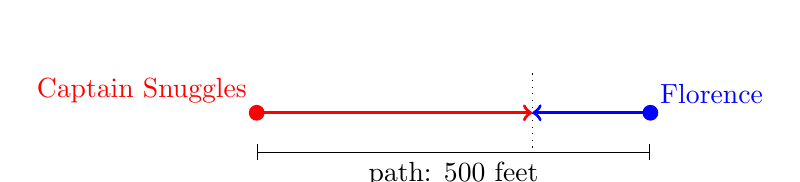
\begin{tikzpicture}
	\draw[|-|] (0,0) -- node[below]{path: 500 feet} (5,0);
	\draw[dotted] (3.5,1) -- (3.5,0);
	% gorilla
	\draw[red, very thick, ->] (0,0.5) -- (3.5,0.5);
	\fill[red] (0,0.5) circle[radius=0.1cm] node[above left]{Captain Snuggles};
	% zookeeper
	\draw[blue, very thick, ->] (5,0.5) -- (3.5,0.5);
	\fill[blue] (5,0.5) circle[radius=0.1cm] node[above right]{Florence};
\end{tikzpicture}
\end{center}%{figure}

The problem asks a question about time, so let's use $t$ to represent the time (in seconds) it takes for the two travelers to meet.

What else do we know from the problem? We have the speeds that both of the characters are moving.\footnote{We are also given the weight of the gorilla, although this is just a distraction and not important to the problem.} Florence moves at a speed of 4 feet per second, so in $t$ seconds she can travel $4t$ feet. Captain Snuggles can travel $26t$ feet in $t$ seconds. So, we can update our picture:
\begin{center}%{figure}
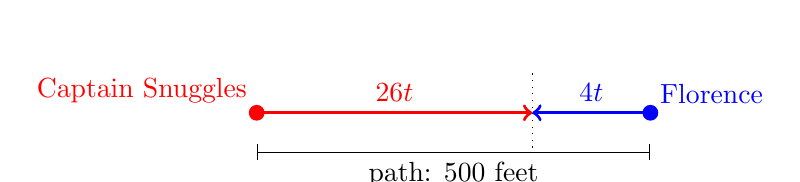
\begin{tikzpicture}
	\draw[|-|] (0,0) -- node[below]{path: 500 feet} (5,0);
	\draw[dotted] (3.5,1) -- (3.5,0);
	% gorilla
	\draw[red, very thick, ->] (0,0.5) -- node[above]{$26t$} (3.5,0.5);
	\fill[red] (0,0.5) circle[radius=0.1cm] node[above left]{Captain Snuggles};
	% zookeeper
	\draw[blue, very thick, ->] (5,0.5) -- node[above]{$4t$} (3.5,0.5);
	\fill[blue] (5,0.5) circle[radius=0.1cm] node[above right]{Florence};
\end{tikzpicture}
\end{center}%{figure}

From the drawing we can see that the combined distance that the two characters travel must be exactly 500 feet! So, we have our equation:
\[26t + 4t = 500\]
Again, we've got just a single linear equation and not a system. Who would have thought that such a complicated-looking problem would have a relatively simple mathematical representation!

%The problem is asks when Yeardleigh will pass Bob. In order to know when she will pass, we need to know when they have gone exactly the same amount of distance from the factory (this is the moment she passes him). So we'll write two distance equations, one for Bob and one for Yeardleigh, and compare them to try and figure out at what time their distances from the factories are equal.
%
%Our table columns are -- naturally enough -- rate, time, and distance. The rows deal with the people driving. The problem asks a ``when'' question, so we must be solving for time. Let's use $t$ to represent the amount of time Bob has been driving, in hours.
%
%Note that we didn't make the variable represent actual time ``on the clock''. (Why not? What challenges would that introduce into the mathematics?)
%


%%%%%%%%%%%%%%%%%%%%%%%%%%%%%%%%%%%%%%%%%%%%%%%%%%

\subsubsection{A trickier RTD problem}

\begin{boxex}
Florence the zookeeper, sadly, found herself on the business end of a hungry gorilla. Luckily, this occurred just outside the security hut, where the zoo's security squad witnessed the terrifying (but non-fatal) mauling. When they sounded the alarm, Captain Snuggles fled toward the zoo's entrance. The security squad gave chase along the same route 30 seconds later, after arming their tranquilizer guns and mounting their bicycles.

Captain Snuggles ran at 18 miles per hour. The security team cycled at 25 miles per hour, which was just fast enough: they reached the zoo entrance at the same moment as the gorilla and tranquilized him into submission. How much time elapsed between the sounding of the alarm and the tranquilizing of the gorilla? How far was the security hut from the zoo entrance?
\end{boxex}

Since the security squad started 30 seconds later, they have 30 seconds less travel time than Captain Snuggles. If we let $t$ represent the amount of time that Captain Snuggles is running (in seconds), then the security squad is chasing for $t-30$ seconds.

Even though Captain Snuggles has a head start, the security squad reaches the entrance at the same time as the gorilla because of their greater speed. So, both parties travel the same distance $d$.

Now, we have to be careful about units! The speeds in this problem are given in \emph{miles per hour}, and the time difference is given in \emph{seconds}. So, we could be careful to keep our units aligned. Let's use a little dimensional analysis (from \cref{ch:proportions}) to convert the speeds to ``feet per second''.\footnote{Alternatively, we could let $t$ represent time in minutes, and then convert the given speeds to distance \textit{per minute}. In that case, the security team would be in pursuit for $t=\frac{1}{2}$ minutes, since 30 seconds is half of one minute.}
\[
\begin{array}{r >{\displaystyle}l}
\text{Captain Snuggles:\quad}
&
\frac{18 \text{ miles}}{\text{hour}}
\cdot
\frac{5280 \text{ feet}}{\text{mile}}
\cdot
\frac{1 \text{ hour}}{3600 \text{ seconds}}
=
\frac{26.4 \text{ feet}}{\text{second}}
\\[\fracspace]
\text{Security Squad:\quad}
&
\frac{25 \text{ miles}}{\text{hour}}
\cdot
\frac{5280 \text{ feet}}{\text{mile}}
\cdot
\frac{1 \text{ hour}}{3600 \text{ seconds}}
=
\frac{36.\overline{6} \text{ feet}}{\text{second}}
\end{array}
\]

If we let $d$ represent the distance (in feet) from the security hut to the zoo entrance, then we can write an equation to describe the motion of Captain Snuggles:
\[d = 26.4t.\]
We can also model the motion of the security squad. Our formula shows both the different speed, and the fact that they start 30 seconds late:
\[d=36.\overline{6}(t-30).\]
These two equations comprise our system. Since we know that the security team and the gorilla arrive at the zoo at the same moment, we know that they travel the same amount of distance. In other words, $d$ is the same for both travelers. Substitution looks like a good choice for solving this system! (Can you explain why?)

%
%\begin{center}
%\begin{tabular}{r|ccc}
%				& Rate (mph)			& Time (hours)		& Distance (miles)\\\hline
%Bob				& 25					& $t$				& $25t$\\
%Yeardleigh		& 40					& $t - \frac{1}{2}$	& $40\left(t - \frac{1}{2}\right)$\\
%\end{tabular}
%\end{center}
%
%\[
%\left\{%
%\begin{aligned}
%&d = 25t\\
%&d = 40\left(t-\frac{1}{2}\right)
%\end{aligned}
%\right.
%\]
%
%Solving this system (substitution looks like a good choice!) will give us a value for $t$. What does that value represent? How can we use it to determine when (on the clock) Yeardleigh will pas Bob?


% % % % % % % % % % % % % % % % % % % % % % % % % % % % % % % % % % % % % % % %
\subsection{Motion in a current}

%Don't let that complicated-sounding name fool you, problems of this type are not that complicated to solve.

Have you ever tried to walk \textit{up} the \textit{down} escalator at the mall? (Be honest!) When you walk down the down elevator -- that is, when you walk in the same direction that the escalator is moving -- the motion of the escalator helps you to go faster than if you were just walking down regular stairs. On the other hand, if you try walk in the wrong direction on an escalator, the motion of the escalator will make you go slower than you would walk on regular stairs.

This is the idea of motion in a current. When you go ``with the current'' (or ``downstream'', if you're floating on a river) the current adds to your usual rate of motion. Going ``against the current'' (or ``upstream''), the current reduces your usual rate of motion.

%Bob decides to go on vacation. He takes a day trip on a river boat. The boat travels 60 km upstream (against the current) in 5 hours. The boat travels the same distance downstream in 3 hours. What is the rate of the boat in still water? What is the rate of the river's current?

\begin{boxex}
Bob and Yeardleigh were at the Cheeseville Zoo on a school field trip at the time of the mauling. When the alarm sounded, they both ran towards the escalators leading up the side of Mount Ploom toward the aviary. Yeardleigh, of course, ran up the up escalator. Bob, in a panic (and, well, because he's Bob), ran up the down escalator.

Yeardleigh reached the top in 19 seconds and Bob reached the top 23 seconds later. If the escalators are each 213 feet long, how fast were the twins running? How fast were the escalators moving? (Assume that the twins run at the same speed, and the two escalators move at the same speed.)
\end{boxex}

In this problem, we don't know either of the speeds. So, let's use $r$ to represent the running speed of the twins and $e$ to represent the moving speed of the escalators.

When Yeardleigh runs with the help of the escalator, she attains a speed of $r+e$. Bob, on the other hand, has his overall speed reduced by the movment of the escalator and moves at a speed of $r-e$.

\begin{center}
\begin{tabular}{r|ccc}
	& Rate (ft/sec)			& Time (sec)		& Distance (ft)\\\hline
Yeardleigh	& $r+e$		& 19			& 213\\
Bob			& $r-e$			& 42			& 213\\
\end{tabular}
\end{center}
Be sure to read carefully! Notice that the problem says Bob reaches the top 23 seconds \emph{later} than Yeardleigh. That means the trip takes him $19+23=42$ seconds. 

%Notice that Bob makes a round trip journey. So, the distance upstream is the same as the distance downstream. We don't know the speed of the water or the speed of the boat. So, let's let $b$ represent the speed of the boat, and $c$ represent the speed of the current.
%
%The boat goes $b-c$ km/hour upstream, because the current is taking away from how fast the boat can go. The boat will go $b+c$ km/hour downstream, because the current will help the boat go faster!
%
%\begin{center}
%\begin{tabular}{r|ccc}
%				& Rate (km/h)			& Time (hours)		& Distance (km)\\\hline
%Upstream		& $b-c$				& 5					& 60\\
%Downstream	& $b+c$				& 3					& 60\\
%\end{tabular}
%\end{center}
%
Given this setup, our system is:
\[
\left\{%
\begin{aligned}
&19(r+e) = 213\\
&42(r-e) = 213
\end{aligned}
\right.
\]
To solve this, we'll need the distributive property and the elimination method!


% % % % % % % % % % % % % % % % % % % % % % % % % % % % % % % % % % % % % % % % 
\chaptersummary

We learned a number of techniques in this section for writing and solving systems of linear equations -- graphing, substitution, and elimination -- and we now have all three approaches in our algebraic toolbox. Each of the techniques has its advantages and disadvantages, but together they make a powerful collection.

In the next chapter we will broaden our algebraic vocabulary, so to speak, by dropping the requirement that we always talk about \textit{equations}, or systems of \textit{equations}. Equality is important (in mathematics and in life), but we all know that things are not always in perfect balance. Onward!

\bigskip
\begin{boxcheese}
Florence the zookeeper made a full recovery, and Captain Snuggles successfully completed an anger management course and was reintroduced to the Cheeseville Zoo community. Unfortunately, the day's events were a public relations nightmare for the zoo. Annual attendance declined exponentially until 2003, at which point the zoo was purchased by YeardleighCorp.
\addtodoitem{Adjust year of YCorp takeover of Cheeseville Zoo.}
\end{boxcheese}

\chaptercopyright

%%%%\include{ch09_inequalities}
%%%%\include{ch10_expofunc}
%%%%\include{ch11_expoexpr}
%%%%\chapter{Quadratic equations}
\label{ch:quadeq}

\chapquote{We must say that there are as many squares as there are numbers.}{Galileo Galilei, Italian physicist and astronomer}

We saw quadratic patterns for the first time back in \cref{ch:sequences}, when we learned about quadratic sequences. We worked a bit with equations for quadratic data, but we haven't seen quadratic equations since then.\footnote{By the way, now might be a good time to have a second look at the final sections of \cref{ch:sequences}. Those are (;,;) sections, and so they may have been a bit challenging the first time around. You have a lot more algebra skills at this point in the course, though, and those sections might not be as daunting now!}

In \cref{ch:equations} we learned a set of tools in for solving linear equations. Many of those tools will be helpful here, but in this chapter, we'll also see what makes quadratic equations different from those we've studied until now. Our main task will be to develop techniques that will help us to overcome the trickier aspects of quadratic equations.

% % % % % % % % % % % % % % % % % % % % % % % % % % % % % % % % % % % % % % % % 
\section{Challenges to solving quadratics}

\begin{boxexplore}[A problem with quadratics]
Consider the following equation. Do we know what we need to know to solve this equation, without any guesswork? In other words: Do we have POEs, axioms, or other properties that will allow us to isolate $x$?
\[x^2 + 2x - 15 = 20\]
If you can, solve the equation. Otherwise, identify where you get stuck. What new tools would be helpful for solving this equation?
\end{boxexplore}

Our task in this chapter is to be able to solve quadratic equations like the one given in the startup exploration. We won't give the details for how to solve this equation yet -- we'll develop those ideas over the next few sections. For now, we will simply point out a few features.

Using what we know so far, it's impossible to isolate $x$. We can make some progress:
\[\begin{aligned}
x^2 + 2x - 15 &= 20
\\
x^2 + 2x &= 35
&&\quad\text{APOE, to get all the numbers to the right-hand side}
\end{aligned}\]
But now what? We can't combine like terms on the left-hand side, and subtracting anything from that side would give us $x$'s on both sides of the equation (making things worse). We might try undoing the distributive property on the left-hand side. That would give us
\[x(x+2)=35.\]
But this doesn't seem to be much of an improvement either. Using DPOE on the left-hand side to isolate $x$ would move $(x+2)$ to the right hand side of the equation (and vice versa). It seems that we'll need some other techniques to help us out of this situation.

If we're allowed to just solve the equation my making a clever observation, we might notice that \[5(7) = 5(5+2)=35,\] and so $x=5$ is a solution to the equation! That's progress. But, it might not be obvious that $-7$ is \textit{also} a solution to the equation, since \[-7(-7+2) = -7(-5) = 35.\] Plus with a different equation, it might not be quite so easy to see a solution just by inspection. What to do with $x(x+2)=29$, for example? Our new techniques should help us overcome these challenges.

\subsection{Rectangles and squares}

As we saw in \cref{ch:sequences}, quadratic sequences can be related to rectangles and squares. Our very first quadratic sequence was related to rectangles (\cref{fig:rects}), and so are the familiar perfect squares (\cref{fig:squares}).

\begin{figure}[!htbp]
\centering
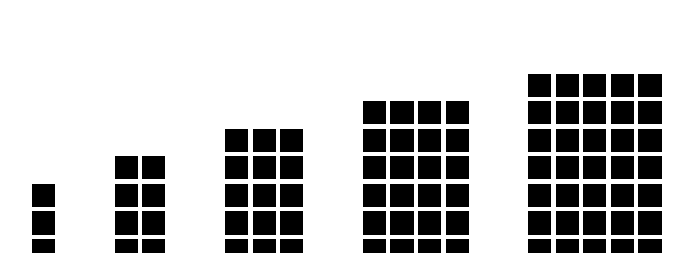
\begin{tikzpicture}[scale=0.35]
	\foreach \x in {0}
	\foreach \y in {0,...,2}
	\draw [ultra thick, white, fill=black] (\x,\y) rectangle (\x+1,\y+1);

	\begin{scope}[xshift=3cm]
	\foreach \x in {0,...,1}
	\foreach \y in {0,...,3}
	\draw [ultra thick, white, fill=black] (\x,\y) rectangle (\x+1,\y+1);
	\end{scope}

	\begin{scope}[xshift=7cm]
	\foreach \x in {0,...,2}
	\foreach \y in {0,...,4}
	\draw [ultra thick, white, fill=black] (\x,\y) rectangle (\x+1,\y+1);
	\end{scope}

	\begin{scope}[xshift=12cm]
	\foreach \x in {0,...,3}
	\foreach \y in {0,...,5}
	\draw [ultra thick, white, fill=black] (\x,\y) rectangle (\x+1,\y+1);
	\end{scope}

	\begin{scope}[xshift=18cm]
	\foreach \x in {0,...,4}
	\foreach \y in {0,...,6}
	\draw [ultra thick, white, fill=black] (\x,\y) rectangle (\x+1,\y+1);
	\end{scope}
\end{tikzpicture}
\caption{Some ``rectangular numbers'': $3, 8, 15, 24, 35, \dotsc$}
\label{fig:rects}
\end{figure}

\begin{figure}[!htbp]
\centering
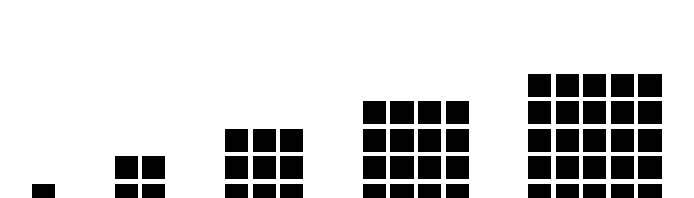
\begin{tikzpicture}[scale=0.35]
	\draw [ultra thick, white, fill=black] (0,0) rectangle (1,1);

	\begin{scope}[xshift=3cm]
	\foreach \x in {0,...,1}
	\foreach \y in {0,...,1}
	\draw [ultra thick, white, fill=black] (\x,\y) rectangle (\x+1,\y+1);
	\end{scope}

	\begin{scope}[xshift=7cm]
	\foreach \x in {0,...,2}
	\foreach \y in {0,...,2}
	\draw [ultra thick, white, fill=black] (\x,\y) rectangle (\x+1,\y+1);
	\end{scope}

	\begin{scope}[xshift=12cm]
	\foreach \x in {0,...,3}
	\foreach \y in {0,...,3}
	\draw [ultra thick, white, fill=black] (\x,\y) rectangle (\x+1,\y+1);
	\end{scope}

	\begin{scope}[xshift=18cm]
	\foreach \x in {0,...,4}
	\foreach \y in {0,...,4}
	\draw [ultra thick, white, fill=black] (\x,\y) rectangle (\x+1,\y+1);
	\end{scope}
\end{tikzpicture}
\caption{The perfect squares: $1, 4, 9, 16, 25, \dotsc$}
\label{fig:squares}
\end{figure}

The perfect squares have a straightforward formula. If we let $f(x)$ represent the area of figure $x$, then the perfect squares are represented by the formula
\[f(x)=x^2.\]
This is the parent function of the quadratic family.

The rectangles in \cref{fig:rects} also have a formula. If we let $g(x)$ represent the area of figure $x$, then we might notice that figure $x$ is $x$ units wide and $(x+2)$ units tall. So these rectangles are represented by the formula
\[g(x) = x(x+2).\]
We can simplify this formula using the distributive property:
\[g(x) = x(x+2) = x^2 + 2x\]

We have learned that the highest degree term in a quadratic equation is an $x^2$ term. The connection between a quadratic rule and rectangles will help us when it comes to solving quadratic equations. In fact, we will solve these equations using the beautiful symmetry of the square.

% % % % % % % % % % % % % % % % % % % % % % % % % % % % % % % % % % % % % % % % 
\section{Level 1 and 2 quadratics}

As we did with linear equations, we'll treat quadratic equations like a game. Level 1 is the easiest kind of quadratic equation to solve, so this is where we'll start. Then, we'll keep things interesting as we increase our skill level by adding challenge and complexity along the way.

\subsection{Level 1 quadratics}

\begin{boxexplore}[Quadratic level 1]
Determine the value of $x$ given the equation: $x^2 = 64$.
\end{boxexplore} %% End of startup exploration

Talk about starting with the easy stuff. We're looking for a number $x$ which, when multiplied by itself, is equal to 64. In other words, we are looking for the ``square root of 64''. Clearly, $x=8$ is a solution to this equation. But we can't be too hasty! Notice that $x=\umin8$ is also a solution, since $(\umin8)^2 = (\umin8)(\umin8) = 64$. So, this equation has two solutions:
\[x = 8 \OR \umin8\]
If we prefer to write our answer in solution set notation, we have \[\solset{8,\umin8}.\]

So, Level 1 quadratics are pretty easy: we simply take the square root of both sides of the equation.\footnote{More soon on square roots, including why and under what circumstances ``square root of both sides'' is, in fact, a property of equality.} We might have a hard time if the constant value is not a perfect square, as in $x^2 = 12$. But, we'll learn more about handling the square roots of non-perfect-squares soon enough (in \cref{ch:radicals}, to be precise).

This seems like a good time to suggest that it may come in handy to memorize the first 25 or so perfect squares, for quick recognition when they come up in a problem.
\begin{align*}
1^2 &= 1		&
2^2 &= 4		&
3^2 &= 9		&
4^2 &= 16		&
5^2 &= 25		\\
6^2 &= 36		&
7^2 &= 49		&
8^2 &= 64		&
9^2 &= 81		&
10^2 &= 100	\\
11^2 &= 121	&
12^2 &= 144 	&
13^2 &= 169 	&
14^2 &= 196 	&
15^2 &= 225 	\\
16^2 &= 256 	&
17^2 &= 289 	&
18^2 &= 324 	&
19^2 &= 361 	&
20^2 &= 400 	\\
21^2 &= 441 	&
22^2 &= 484 	&
23^2 &= 529 	&
24^2 &= 576 	&
25^2 &= 625 	\\
\end{align*}

Finally, note that zero is also a perfect square, since $0^2 = 0$. Zero, in fact, is the only number that has only one square root. Whereas both 3 and $\umin3$ are square roots of 9, the only square root of 0 is 0.

Finally, consider the square root of a negative number, say, $\umin25$. This is a bit of a problem. We're meant to find the the number that when multiplied by itself gives $\umin25$ as the result, but that's not going to work. Since we have a negative product, the two factors must have opposite signs! The best we can do is $5\cdot\umin5 = \umin25$ or $\umin5\cdot5 = \umin25$, and in these cases we're not multiplying a number times itself: 5 and $\umin5$ are different numbers!

So, there is no real number equal to the square root of $\umin25$. Of course, $\umin25$ isn't special, the same argument applies to any negative number. The moral of the story is this: If, as we go about solving a quadratic equation, we come to the point where we need to take the square root of a negative number, we have to stop and say that the equation has ``no real number'' as its solution. $\mathcal{S}=\emptyset$.


\subsection{Level 2 quadratics}

\begin{boxexplore}[Quadratic level 2]
Determine the value of $w$ given the equation: $(w+3)^2 = 16$.
\end{boxexplore} %% End of startup exploration

Here, we're told that something-squared is 16. Well, that means that the something in question must either be 4 or negative 4. That is to say, $(w+3)$ is either 4 or $\umin4$. So, this equation is actually two equations at once. We have:
\[w+3 = 4 \qquad\text{\underline{or}}\qquad w+3 = -4\]
Solving these equations (using SPOE in both cases), we have that $w$ must be either $1$ or $\umin7$. So, those are our two solutions: $\solset{1,\umin7}$.

We can record this work in a down-the-page format, like so:
\begin{align*}
(w+3)^2 &= 16
\\
w+3 &= 4 \OR \umin4
&&\text{square root of both sides}
\\
w &= 1 \OR \umin7
&&\text{SPOE: subtract 3 throughout}
\end{align*}

A few things to note: First, we can't subtract 3 from both sides as the very first step. The parentheses require that we undo the exponent first. Second, beware the use of $\pm$. It may be tempting to use this shorthand notation and write
\begin{align*}
w+3 &= \pm4,\\
\intertext{but then it is also tempting to subtract 3 and write}
w &= \pm1. \quad\text{Nope!}
\end{align*}
We recommend splitting into two equations, or writing out the two solutions explicitly using the word ``or''.

\begin{boxex}
Determine the value of $a$ given the equation: $(a-1)^2 - 2 = 23$.

\exsoln\ This equation requires an extra step, but it's quickly transformed into an equation like the one from the startup exploration.
\begin{align*}
(a-1)^2 - 2 &= 23
\\
(a-1)^2 &= 25
&&\text{APOE}
\\
a-1 &= 5 \OR \umin5
&&\text{square root of both sides}
\\
w &= 6 \OR \umin4
&&\text{APOE: add 1 throughout}
\end{align*}
In the end, we have $\solset{6, \umin4}$.
\end{boxex}

% % % % % % % % % % % % % % % % % % % % % % % % % % % % % % % % % % % % % % % % 
\section{Level 3 quadratics: Quadrangle method}

\begin{boxexplore}[Quadratic level 3]
Use the sum to a power property (from \cref{sec:exposumstopowers}) to write the expression $(x+3)^2$ without parentheses. Then, determine the value of $x$ given the equation: $x^2+6x+9 = 49$.
\end{boxexplore} %% End of startup exploration

To expand $(x+3)^2$, we might think of using algebra tiles to fill in a square with side length $(x+3)$. We used algebra tiles to solve this kind of problem back in \cref{sec:exposumstopowers}. Or, we could just ``sketch'' the algebra tiles diagram (shown below, on the right) and calculate the areas of the four regions.

\begin{minipage}{0.49\linewidth}
\centering
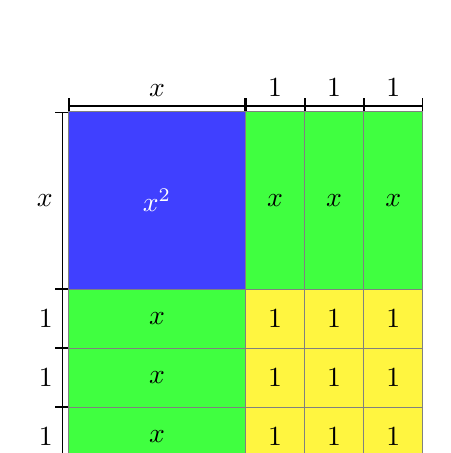
\begin{tikzpicture}[scale=0.75]
	\draw[|-|] (0,0.1) -- node[above]{$x$} (3,0.1);
	\draw[|-|] (-0.1,0) -- node[left]{$x$} (-0.1,-3);
	\draw[gray, fill=blue!75] (0,0) rectangle node[white]{$x^2$} (3,-3);
	\foreach \x in {3,...,5} {
		\draw[|-|] (\x,0.1) -- node[above]{1} (\x+1,0.1);
		\draw[gray, fill=green!75] (\x,0) rectangle node[black]{$x$} (\x+1,-3);
	}
	\foreach \y in {-3,...,-5} {
		\draw[|-|] (-0.1,\y) -- node[left]{1} (-0.1,\y-1);
		\draw[gray, fill=green!75] (0,\y) rectangle node[black]{$x$} (3,\y-1);
	}
	\foreach \x in {3,...,5} {
		\foreach \y in {-3,...,-5}
			\draw[gray, fill=yellow!75] (\x, \y) rectangle node[black]{1} (\x+1,\y-1);
	}
\end{tikzpicture}
\end{minipage}
%%
\begin{minipage}{0.49\textwidth}
	\quadrangle{x}{3}{x^2}{3x}{9}
\end{minipage}

Note how we have simplified the picture in the ``sketch'' version. For example, rather than draw three 3-unit-by-$x$-unit rectangles, we simply write the area of the rectangle $3x$. In the lower right-hand region, we write the area 9 rather than draw nine yellow squares.

We'll call this simplified sketch a \textit{quadrangle diagram}, and we'll call the method we are developing here the \textit{quadrangle method}.\footnote{The term \textit{quadrangle} is a synonym for \textit{rectangle}. History suggests that the term \textit{quadratic} is related to the term \textit{quadrangle} since this method of using square diagrams is so helpful in solving quadratic equations.} The quadrangle diagram can help us to see the relationship between the two expressions in the startup exploration:
\[(x+3)^2 = x^2 + 6x + 9.\]
Using this fact, we can solve the given equation:
\begin{align*}
x^2 + 6x + 9 &= 49
\\
(x+3)^2 &= 49
&&\text{based on the quadrangle diagram}
\\
x+3 &= 7 \OR \umin7
&&\text{square root of both sides}
\\
x &= 4 \OR \umin10
&&\text{SPOE: subtract 3 throughout}
\end{align*}
Can you see the clever trick that we used here? We rewrote an expanded expression as a something-squared expression, and then we solved it like a Level 2 quadratic!

Let's work through another example in detail, for example, solving the Level 3 equation
\[x^2 + 12x + 36 = 144.\]

Our goal is to write the left-hand side in a something-squared form. To do that, we'll begin by drawing an empty quadrangle diagram and filling in the bits that we know. For example, we know that the upper left-hand box must contain $x^2$, and so the sides of that square must each be $x$ units long.

\quadrangle{x}{}{x^2}{}{}

We know that the 36 will appear in the lower right-hand box. But how sould we label the side lenghts here? There are lots of combinations of numbers that multiply together to get 36\ldots

\quadrangle{x}{?}{x^2}{}{36}

Remember that the goal is to get an expression of the form something-\textit{squared}, and so we should always strive to create a quadrangle that is, in fact, a square. This means that we must choose 6 and 6 as the side lengths. If we chose another pair of factors, like 2 and 18, we would get the proper product in the lower right-hand region, but our overall diagram would no longer be a square.

\quadrangle{x}{6}{x^2}{}{36}

To fill in the remaining regions, we multiply the dimensions of each. In both cases we get $6x$. This is good news! Together these make $12x$ (which is what we have in the original, expanded expression). Plus, the two regions contain the same value, and so the beautiful symmetry of the square is preserved.

\quadrangle{x}{6}{x^2}{6x}{36}

So, we have rewritten our expression as a something-squared expression:
\[x^2 + 12x + 36 = (x+6)^2.\]
We can use this to solve the equation that we were given:
\begin{align*}
x^2 + 12x + 36 &= 144
\\
(x+6)^2 &= 144
&&\text{based on the quadrangle diagram}
\\
x+6 &= 12 \OR \umin12
&&\text{square root of both sides}
\\
x &= 6 \OR \umin18
&&\text{SPOE}
\end{align*}

\begin{boxex}
Determine the value of $n$ given the equation: $n^2 - 16n + 64 = 1$.

\exsoln\ Let's build the quadrangle diagram. The upper left-hand corner contains $n^2$, as above. To maintain symmetry, we should split the $-16n$ exactly in half. Don't worry about the negative coefficient, we can work with that. We should be on guard though for sign-related issues.

\quadrangle{n}{}{n^2}{-8n}{}

This tells us that the remaining portion of the square's side length must be $-8$. Let's not worry too much about the fact that negative distances are impossible\ldots\ the idea still works. This implies that the remaining region contains 64 (note, that positive 64). This agrees with the equation we were given.

\quadrangle{n}{-8}{n^2}{-8n}{64}

Now, we can solve the equation:
\begin{align*}
n^2 -16n +64 &= 1
\\
(n-8)^2 &= 1
&&\text{based on the quadrangle diagram}
\\
n-8 &= 1 \OR \umin1
&&\text{square root of both sides}
\\
n &= 9 \OR 7
&&\text{SPOE}
\end{align*}
So, we have $\solset{7,9}$. We can check our work by substituting our proposed solutions back into the original equation. First, we'll test $n=7$:
\begin{align*}
n^2 -16n +64 &= 1
\\
(7)^2 - 16(7) + 64 &\overset{?}{=} 1
\\
49 - 112 + 64 &\overset{?}{=} 1
\\
1 &\overset{\checkmark}{=} 1
\end{align*}
First, we'll check $n=9$:
\begin{align*}
n^2 -16n +64 &= 1
\\
(9)^2 - 16(9) + 64 &\overset{?}{=} 1
\\
81 - 144 + 64 &\overset{?}{=} 1
\\
1 &\overset{\checkmark}{=} 1
\end{align*}
\end{boxex}

% % % % % % % % % % % % % % % % % % % % % % % % % % % % % % % % % % % % % % % % 
\section{Level 4 quadratics: Adjust the constant term}

\begin{boxexplore}[Quadratic level 4]
Determine the value of $x$ given the equation: $x^2 + 8x + 15 = 99$.
\end{boxexplore} %% End of startup exploration

Let's try to build the quadrangle diagram. The upper left-hand corner contains $x^2$, as before. To maintain symmetry, we should split the $8x$ exactly in half. This tells us that the large square must be $(x+4)$ units on a side.

\quadrangle{x}{4}{x^2}{4x}{}

The problem is that, according to our quadrangle diagram, the lower right-hand corner should be 16\ldots\ but the equation we are given tells us to put 15 in that space. Now what? Our equation does not represent a complete square!

\quadrangle{x}{4}{x^2}{4x}{\color{red}15}

POEs to the rescue! Why not add 1 to both sides of the given equation to complete the square? This will give us the number we want on the left-hand side and, since we add 1 to both sides, we have an equivalent equation. So, instead of solving the equation
\[x^2 + 8x + 15 = 99,\]
we will add one to both sides and solve the equation
\[x^2 + 8x + 16 = 100.\]
Now, we can draw the quadrangle diagram exactly as we wanted.

\quadrangle{x}{4}{x^2}{4x}{16}

And now that we have a proper quadrangle diagram, we can solve the equation! Here's the full process:
\begin{align*}
x^2 + 8x + 15 &= 99
\\
x^2 + 8x + 16 &= 100
&&\text{APOE: add 1 to both sides}
\\
(x+4)^2 &= 100
&&\text{based on the quadrangle diagram}
\\
x+4 &= 10 \OR \umin10
&&\text{square root of both sides}
\\
x &= 6 \OR \umin14
&&\text{SPOE}
\end{align*}

This is a clever application of the POEs. Rather than use the properties to eliminate terms from one side of the equation, we can use the properties to change one side into a particular, more-helpful form.\footnote{In fact, this is exactly what we've been doing all along: changing one side of an equation into a form that is more helpful. In this chapter we are expanding our notion of what it means for a change to be ``helpful''.}

\begin{boxex}
Determine the value of $x$ given the equation: $x^2-6x+11=27$.

\exsoln\ When we start the quadrangle diagram, we split the $-6x$ as usual. This means that the square has sides of length $(x-3)$. This, in turn, implies that the lower right-hand region should be 9. Our equation has 11 as its constant term: not what we want.

\quadrangle{x}{-3}{x^2}{-3x}{\color{red}9}

To fix, this we can subtract 2 to each side of our equation. This will give us a constant term of 9, which is what we need to make our quadrangle diagram work. So, we have:
\begin{align*}
x^2 - 6x + 11 &= 27
\\
x^2 - 6x + 9 &= 25
&&\text{SPOE: subtract 2 from both sides}
\\
(x-3)^2 &= 25
&&\text{based on the quadrangle diagram}
\\
x-3 &= 5 \OR \umin5
&&\text{square root of both sides}
\\
x &= 8 \OR \umin2
&&\text{SPOE}
\end{align*}
So, our solutions are $\solset{8, \umin2}$.
\end{boxex}

% % % % % % % % % % % % % % % % % % % % % % % % % % % % % % % % % % % % % % % % 
\section{Level 5 quadratics: Adjust the linear term}

The last few levels have had ``polite'' middle terms, which have split evenly into two pieces. What happens if we get a linear term with an odd coefficient?

\begin{boxexplore}[Quadratic level 5]
Determine the value of $x$ given the equation: $x^2 + 3x + 1 = 5$.
\end{boxexplore} %% End of startup exploration

If we jump right in and try the quadrangle method, we start to get into fraction territory. If we want to split the $3x$ term exactly in half, then each piece would be $\frac{3}{2}$. Then, the quadrangle method would predict $\frac{9}{4}$ in the lower-right corner.

\quadrangle{x}{\frac{3}{2}}{x^2}{\frac{3}{2}x}{\color{red}\frac{9}{4}}

The lower-right corner isn't what we have in our equation, so we could use APOE and add $\frac{5}{4}$ to adjust both sides\ldots\ Hmm. Not pretty. To be clear, the quadrangle method will not let us down: if we keep going with the fractions, we will arrive at the correct answer! But, perhaps there is an alternative approach that avoids the fractions.

Here's a clever idea: We could use MPOE and multiply through by 2. This would give us a linear term with an even coefficient! In other words:
\[x^2 + 3x + 1 = 5 \quad\xrightarrow{\quad\text{multiply through by 2}\quad}\quad 2x^2 + 6x + 2 = 10\]
This fixes our odd coefficient problem, since now we can break the $6x$ up into two sets of $3x$. But, what do we do with that $2x^2$? We can't use $x$ and $2x$ as the side lengths, for although that gives is the correct product, we would no longer have a square.

\quadrangle{\color{red}?}{3}{2x^2}{3x}{}

Now, here's a \textit{really} clever idea. Let's multiply through by 2 \textit{again}. In other words, we will multiply the original equation by 4:
\[x^2 + 3x + 1 = 5 \quad\xrightarrow{\quad\text{multiply through by 4}\quad}\quad 4x^2 + 12x + 4 = 20\]
We still have an even linear coefficient, and now we can write $4x^2$ as $2x$ times $2x$. Note that we have to take that factor of 2 into account when we're figuring out the other dimensions of the square. Study our new diagram closely and be sure you understand where each of the labels comes from.
\begin{center}
	\quadrangle{2x}{3}{4x^2}{6x}{9}
\end{center}

We now find ourselves in a Level 4 situation: our equation has 4 as the constant term, whereas the quadrangle diagram predicts 9 as the constant term. No problem! We can add 5 to both sides, and continute the process as we did with Level 4 quadratics. Here's a summary of the whole process:
\begin{align*}
x^2 + 3x + 1 &= 5
&&\text{original equation}
\\
4x^2 + 12x + 4 &= 20
&&\text{MPOE: multiply both sides by 4}
\\
4x^2 + 12x + 9 &= 25
&&\text{APOE: add 5 to both sides}
\\
(2x+3)^2 &= 25
&&\text{based on the quadrangle diagram}
\\
2x+3 &= 5 \OR \umin5
&&\text{square root of both sides}
\\
2x &= 2 \OR \umin8
&&\text{SPOE}
\\
x &= 1 \OR \umin4
&&\text{DPOE}
\end{align*}

Let's pause and review. When faced with an odd coefficient for the $x$ term, our strategy is to multiply through by 4. This will give us an even coefficient for the $x$ term, and at the same time keep the coefficient of the $x^2$ term in a state where it can be written as something times itself: $4x^2 = 2x\cdot2x$. After we do this, we'll have a Level 4 quadratic on our hands, and we can apply techniques for handling those.

\begin{boxex}
Determine the value of $x$ given the equation: $x^2-5x+12=62$.

\exsoln\ Faced with an odd linear coefficient, we multiply through by 4. This gives us the revised equation \[4x^2-20x+48=248.\] We set up the quadrangle diagram and see whether our equation represents a complete square.

\quadrangle{2x}{-5}{4x^2}{-10x}{\color{red}25}

Our (revised) equation does not make a proper square: the constant term in the equation is 48, but the quadrangle diagram predicts 25. We can fix this problem using SPOE: subtract 23 from both sides:
\begin{align*}
x^2 - 5x + 12 &= 62
&&\text{original equation}
\\
4x^2 - 20x + 48 &= 248
&&\text{MPOE: multiply both sides by 4}
\\
4x^2 - 20x + 25 &= 225
&&\text{SPOE: subtract 23 from to both sides}
\\
(2x-5)^2 &= 225
&&\text{based on the quadrangle diagram}
\\
2x-5 &= 15 \OR \umin15
&&\text{square root of both sides}
\\
2x &= 20 \OR \umin10
&&\text{SPOE}
\\
x &= 10 \OR \umin5
&&\text{DPOE}
\end{align*}
So in the end, we have solutions $\solset{10, \umin5}$.
\end{boxex}

% % % % % % % % % % % % % % % % % % % % % % % % % % % % % % % % % % % % % % % % 
\section{Level 6 quadratics: Adjust the quadratic term}

We've arrived at the highest level of the quadratic equation challenge! Until now, all of our equations have started with just $x^2$. What if the coefficient of the leading term is something other than 1?

\begin{boxexplore}[Quadratic level 6]
Determine the value of $x$ given the equation: $3x^2 + 8x + 1 = 12$.
\end{boxexplore} %% End of startup exploration

What shall we do in this scenario? A clever idea is to use DPOE and divide through by 3. That would make the leading coefficient 1, as in the earlier problems. The downside is that most of the other numbers turn into fractions.
\[3x^2 + 8x + 1 = 12
\quad\xrightarrow{\quad\text{divide through by 3}\quad}\quad
x^2 + \frac{8}{3}x + \frac{1}{3} = 4\]
The quadrangle method will absolutely work on an equation like this, but perhaps we'd prefer an approach that avoided all the fractions.

If scaling the equation down doesn't help, why not try to scale it up? Could we multiply through by some helpful value? Recall that the goal will be to write the $x^2$ term as something times itself. Since there's already a 3 there, we can solve our problem if we multiply through by 3.
\[3x^2 + 8x + 1 = 12
\quad\xrightarrow{\quad\text{multiply through by 3}\quad}\quad
9x^2 + 24x + 3 = 36\]
Note that now we are in a good position, since $9x^2 = 3x\cdot3x$. So, let's fill out our quadrangle diagram. We have an even coefficient on the linear term, so we can split that evenly. Note that we have to take all the coefficients into account when completing the diagram. For example, when figuring out the dimensions of a box containing $12x$.

\quadrangle{3x}{4}{9x^2}{12x}{\color{red}16}

The quadrangle diagram predicts 16 as the constant term, and so our equation is not a complete square. We can use APOE to fix that, adding 13 to both sides. Here's how it goes:
\begin{align*}
3x^2 +8x + 1 &= 12
&&\text{original equation}
\\
9x^2 + 24x + 3 &= 36
&&\text{MPOE: multiply through by 3}
\\
9x^2 +24x + 16 &= 49
&&\text{APOE: add 13 to both sides}
\\
(3x+4)^2 &= 49
&&\text{based on the quadrangle diagram}
\\
3x+4 &= 7 \OR \umin7
&&\text{square root of both sides}
\\
3x &= 3 \OR \umin11
&&\text{SPOE}
\\
x &= 1 \OR \umin\tfrac{11}{3}
&&\text{DPOE}
\end{align*}

In summary, we multiplied through by the coefficient of the $x^2$ term, which gave us a coefficient that was a perfect square. In the final example for this chapter, we put it all together.

\begin{boxex}
Determine the value of $x$ given the equation $-5x^2-x+18=0$.

\exsoln\ Since we have a leading coefficient that is not a perfect square, we multiply through by that coefficient, $-5$ in this case. This gives us
\[25x^2+5x-90=0\]
(careful with the negative signs). This is an improvement, but we have a linear coefficient that is odd. So, we multiply by 4 to fix that:
\[100x^2 + 20x - 360=0\]
Notice that multiplying through by 4 (a perfect square) gives us a leading coefficient that is still a perfect square. This is because the product of two perfect squares is itself a perfect square! (Can you prove that this statement is always true using the properties of exponents?)

We now have a revised equation that we can bring to the quadrangle method.

\quadrangle{10x}{1}{100x^2}{10x}{\color{red}1}

To get our constant terms to agree, we must add 361 to both sides of our revised equation. This gives us
\[10x^2 + 10x + 1 = 361.\]
And from here, we can complete a familiar process.
\begin{align*}
10x^2 +10x + 1 &= 316
&&\text{}
\\
(10x+1)^2 &= 316
&&\text{based on the quadrangle diagram}
\\
10x+1 &= 19 \OR \umin19
&&\text{square root of both sides}
\\
10x &= 18 \OR \umin20
&&\text{SPOE}
\\
x &= \tfrac{18}{10} \OR \umin2
&&\text{DPOE}
\end{align*}
After we simplify our one fraction answer, we have a final solution: $\solset{\frac{9}{5}, \umin2}$.
\end{boxex}

\subsection{(;,;) Quadratic formula}
\label{sec:quadformulapreview}

Now that we have the quadrangle method at our disposal, we can tackle any quadratic equation that is thrown at us. We might be tempted to really get generic, and solve the all at once.

Consider a completely generic quadratic equation of the form \[ax^2 + bx + c=0.\] This quadratic has three coefficients: $a$ is the coefficient of the quadratic term, $b$ is the coefficient of the linear term, and $c$ is the constant term. We've set it equal to zero for reasons that will be made clear in a few chapters.\footnote{Sorry for the mystery, but all will be revealed soon. In the meantime, note that we can always turn a quadratic equation into this form. If we have an equation that does not equal zero, for example $ax^2 + bx + c = d$ where $d$ is not zero, then we can use SPOE to get 0 on the right-hand side: $ax^2+bx+c-d=0$. Then, we pull a little algebraic sleight of hand, and replace $c-d$ with just $c$. This might look like an illegal move, but in the general form of a quadratic, ``$c$'' just stands for a constant value. Since ``c-d'' is a contstant value, we pretend that this was the constant value we meant all along.}

What happens if we apply the quadrangle method to this totally generic equation? We don't really know anything about $a$, so to be safe, let's multiply the whole equation by $a$. 
\[a^2x^2 + abx + ac=0.\]
This will ensure that the leading term is a perfect square, and that's what we need for the box method. Now, the linear coefficient is $ab$ and this might be an odd number for all we know. So, we multiply through by 4, as we have often done above.
\[4a^2x^2 + 4abx + 4c=0.\]
This is not a pretty sight, but we'll try to make it work with the quadrangle method.

\quadrangle{2ax}{b}{4a^2x^2}{2abx}{\color{red}b^2}

Much of this looks workable, but what about the lower right-hand corner? The quadrangle method predicts $b^2$, but our equation has $4c$. Well, we'll do what we usually do: we'll use the POEs to turn our left-hand side into the form we want. So:

\begin{align*}
4a^2x^2 + 4abx + 4c &= 0
&&\text{}
\\
4a^2x^2 + 4abx &= -4c
&&\text{SPOE: subtract $4c$ from both sides}
\\
4a^2x^2 + 4abx +b^2 &= b^2-4c
&&\text{APOE: add $b^2$ to both sides}
%
\intertext{It might seem like things are getting worse, but now the left-hand side is what we need to use our quadrangle diagram. Let's go!}
%
(2ax+b)^2 &= b^2-4c
&&\text{based on the quadrangle diagram}
\\
2ax+b &= \pm\sqrt{b^2-4c}
&&\text{square root of both sides}
\\
2ax &= \pm\sqrt{b^2-4c}-b
&&\text{SPOE: subtract $b$ from both sides}
\\[1ex]
x &= \frac{\pm\sqrt{b^2-4c}-b}{2a}
&&\text{DPOE: divide both sides by $2a$}
\\[1ex]
x &= \frac{-b\pm\sqrt{b^2-4c}}{2a}
&&\text{rearranging the numerator}
\end{align*}

That last rearrangement in the numerator is because it looks a little better, and to make it clear that the $-b$ isn't underneath the radical along with that other stuff. Also, it's tradition. This formula is a famous thing, and traditionally appears in this form.

% % % % % % % % % % % % % % % % % % % % % % % % % % % % % % % % % % % % % % % % 
\chaptersummary

The properties of equality which we learned before this chapter weren't enough to solve any random quadratic equation. To overcome the quadratic obstacle, we learned new techniques for solving quadratic equations. These new techniques are based on the symmetry of a square, and we learned various techniques for adjusting a quadratic equation so that we can use our new quadrangle method.

We have, however, avoided the necessity of finding the square root of a number that was not a perfect square. This was a helpful simplification -- it allowed us to focus on the process of equation solving -- but not all quadratics will have answers that come out so ``nice''. We turn our attention to square roots in the next chapter.

\chaptercopyright
%%%%\chapter{Radical expressions}
\label{ch:radicals}

\newcommand*\rfrac[2]{{}^{#1}\!/_{#2}}

\chapquote{There is geometry in the humming of the strings, there is music in the spacing of the spheres.}{Pythagoras, Ancient Greek philosopher}

In the last chapter, we found integer solutions to nearly all of the equations that we studied. This was good for understanding the workings of quadratic equations, but not all equations will necessarily be so ``polite''. The main focus of our work in this chapter is around understanding more about all of those square roots that don't come out evenly. We begin by looking more closely at the sets $\Q$ and $\R$.

% % % % % % % % % % % % % % % % % % % % % % % % % % % % % % % % % % % % % % % % 
\section{Real numbers}
\label{sec:radrealnumbers}

\begin{boxexplore}[Share the cheese]
Middle Market sells mini-wheels of cheese for snacking. Mini-wheels can be sold one at a time, or in boxes of 10. The cheese arrives at the warehouse in crates of 10 boxes (containing 100 wheels of cheese in total).

The warehouse workers need to divide their stock of mini-wheels up among three trucks, each of which will deliver to a local Middle Market branch. The warehouse has a total of 13 crates, 7 boxes, and 9 mini-wheels in stock.

The manager allows the workers to open crates or boxes, if needed, to divide the supply evenly. Describe a process for dividing up the cheese that requires opening the minimum number of boxes.
\end{boxexplore}

In \cref{ch:numbers}, we made some comments which might, at first, appear contradictory. On the one hand, we saw that the set of real numbers, $\R$, includes every possible decimal number. We also saw that the set of rational numbers, $\Q$, includes ``terminating decimals and repeating decimals''. 

On the other hand, we know that $\Q$ is the set of fractions, meaning those numbers that can be expressed in the form \[\frac{a}{b} \text{ where $a$ and $b$ are integers, and $b$ is not zero.}\]
These statements raise a few questions. What is the relationship between ``fraction'' and ``terminating or repeating decimal''? What can we say about decimal numbers that are neither terminating nor repeating?

\subsection{Fractions into decimals}

Recall that a fraction is simply a divison problem in disguise. If we execute the division problem, we can easily turn a fraction into a decimal. It's especially easy if we have a calculator handy\ldots\ otherwise, we're in for some long division.

\subsubsection{Long division}

Don't worry if your long division is a bit rusty, just take another look at the startup exploration. The warehouse workers must divide 1379 mini-wheels of cheese among the three trucks (that's $1379 \div 3$) but they must do this with a minimum amount of regrouping.

One solution is to put 4 crates on each of the three trucks. This takes care of 12 crates (1200 mini-wheels in all), but leaves one crate. They have no choice but to open this crate and treat it as 10 boxes. Of course they already had 7 boxes in stock, so now they have 17 boxes in all. They can put 5 boxes on each truck (accounting for 15 boxes, or 150 mini-wheels), but they will have 2 boxes left over. They open these two boxes, revealing 20 mini-wheels. They add these to the 9 mini-wheels they had already, giving 29 mini-wheels in all. Each truck gets 9 of these (using up 27), and they have 2 left over.

So, in the end: each truck gets 4 crates, 5 boxes, and 9 mini-wheels -- that's 459 mini-wheels in all -- and there are 2 left behind. Now have a look at the long division for this problem: can you spot each of the steps that we took above in the work below?

\[
\renewcommand\arraystretch{1.1}
\begin{array}{*1r @{\hskip\arraycolsep}c@{\hskip\arraycolsep} *4r}
	&&			& 4	& 5 & 9\\
\cline{2-6}
3	&\big)&	1	& 3	& 7 & 9\\
	&&		1	& 2	& 0	& 0\\
\cline{3-6}
	&&			& 1	& 7 & 9\\
	&&			& 1	& 5	& 0\\
\cline{4-6}
	&&			& 	& 2	& 9\\
	&&			&	& 2	& 7\\
\cline{5-6}
	&&			& 	& 	& 2\\
\end{array}
\]

In the cheese example, it makes sense to stop here with a remainder of 2. In general, though, we could continue the process of division and create a number that extends to the right of the decimal point.

\begin{boxex}
Convert $\dfrac{3}{4}$ and $\dfrac{1}{6}$ into their decimal representations.

\bigskip\inlineex{Solution:} Recall that the fraction three-fourths is equivalent to the division problem $3 \div 4$. To do this by long division, we put the dividend (that's 3) inside the ``division house'' and leave the divisor (that's 4) outside.
\[
\renewcommand\arraystretch{1.1}
\begin{array}{*1r @{\hskip\arraycolsep}c@{\hskip\arraycolsep} *3r}
	&&			0& .7	& 5 \\
\cline{2-5}
4	&\big)&	3	& .0	& 0 \\
	&&		2	&8		\\
\cline{3-4}
	&&			&2 & 0 \\
	&&			&2 & 0 \\
\cline{4-5}
	&&			&& 0 \\
\end{array}
\]
So the decimal representation of $\frac{3}{4} = 0.75$ (you may have known that already). To tackle one-sixth, we note that it is equivalent to $1 \div 6$. The long division starts out like this:
\[
\renewcommand\arraystretch{1.1}
\begin{array}{*1r @{\hskip\arraycolsep}c@{\hskip\arraycolsep} *4r}
	&&			0& .1	& 6	& 6 \\
\cline{2-6}
6	&\big)&	1	& .0	& 0	& 0 \\
	&&		0	&6		\\
\cline{3-4}
	&&			&4	& 0 \\
	&&			&3	& 6 \\
\cline{4-5}
	&&			&	& 4	& 0 \\
	&&			&	& 3	& 6 \\
\cline{5-6}
	&&			&	&	& 4
\end{array}
\]
We might as well stop here, though, because we're stuck in a loop! The 6's in the answer are going to repeat forever. (Can you see why?) So, the decimal representation of $\frac{1}{6} = 0.1\overline{6}$.
\end{boxex}

We say that $0.75$ is a terminating decimal, because the process of long division stops with a remainder of zero. On the other hand, $0.1\overline{6}$ is called a repeating decimal because the long division process gets stuck in a loop. Note that we've used a vinculum over the 6 to indicate which digits repeat.

When it comes to a division problem like $1 \div 6$ on a calculator, the display will likely show \texttt{0.166666667}, where the 6's repeat for a while and are followed by a 7. Don't be fooled by this 7: the 6's really do go on forever! That 7 is the calculator rounding up. Always be skeptical about the rightmost digit on your calculator screen.

\subsubsection{A bold claim}

This process of division leads us to make a pretty bold claim: every rational number can be represented \textit{either} as a terminating decimal or a repeating decimal. How can we be sure that every crazy fraction, for instance $\frac{19}{81}$, either terminates or repeats?

Let's think about how long division works: the ``subtraction step'' in particular. Here's how the process of long division starts out for $\frac{3}{4}$:
\[
\renewcommand\arraystretch{1.1}
\begin{array}{*1r @{\hskip\arraycolsep}c@{\hskip\arraycolsep} *3r}
	&&			& .7	&	\\
\cline{2-5}
4	&\big)&	3	& .0	& 0 \\
	&&		2	&8		\\
\cline{3-4}
	&&			&2 & 	\\
\end{array}
\]
In the subtraction step, we get 2 as the remainder, and so we know that we have to keep dividing. If we ever get the remainder 0, then we know that we're done with division. This is what happens eventually with $\frac{3}{4}$. On the other hand, if we ever get a remainder that we've gotten before, then we know that we're stuck in a loop. This is what happened with $\frac{1}{6}$.

Now here's a simple yet profound idea: the remainder is always less than the divisor. When dividing by 4, the remainder has to be less than 4. When dividing by 6, the remainder has to be less than 6. (Can you explain why that is? For example, when dividng mini-wheels of cheese among three trucks, could the workers have seven mini-wheels of cheese left over?)

The result is that we have a limited number of choices for the remainder. When dividing by 4, the remainder can only be 0, 1, 2, or 3. When dividing by 6, the remainder can only be : 0, 1, 2, 3, 4, or 5.

Having a limited number of choices means that eventually we have to recycle one of those remainders! We can't go on forever without either using the remainder 0 (in which case the decimal terminates) or reusing one of the nonzero remainders (in which case the decimal repeats).

Even when dividing something ugly like $1903 \div 8167$, the remainders in the subtraction steps will always be less than 8167. We might have to divide for a long time, but we know it can't carry on forever. Eventually we'll either use the remainder 0, or reuse a remainder we've used already. So the fraction $\frac{1903}{8167}$ has a decimal representation that either terminates or repeats.

Our argument applies to any denominator, and so to any rational number. Therefore, it's true that every rational number has a decimal representation that either terminates or repeats! Have we blown your mind yet? If not, stay tuned.

\subsection{Decimals into fractions}

What about the other way around? Does every terminating-or-repeating decimal have a corresponding fraction representation?

\subsubsection{Terminating decimals into fractions}

Consider a terminating decimal like $0.375$. Can we turn this decimal into a fraction, meaning a ratio of two integers? If so, how?

Recall the notion of \textit{place value}, and how the individual digits in a number are each standing in some ``place'' that is named after a power of ten.\footnote{We really are blowing the cobwebs off of some old mathematics in this chapter: Long division! Place value! It goes to show that even simple mathematical ideas can have deep and meaningful consequences.} The key to turning a terminating decimal into a fraction is recalling how to read a decimal using its place value.

\begin{center}
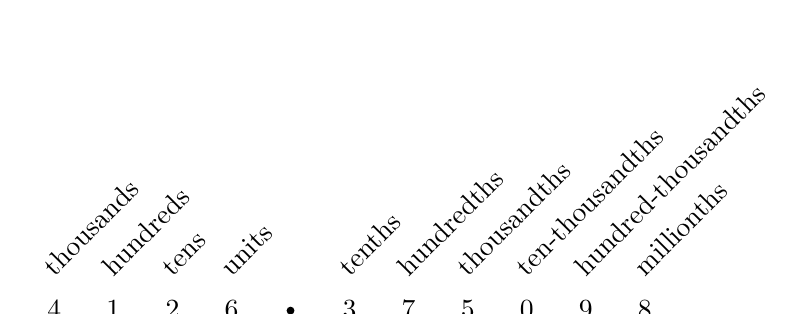
\begin{tikzpicture}
	\foreach \x in {0.75} {
		\draw (-4*\x,0) node[below]{4};
		\draw (-4*\x,0) node[above, anchor=south west, rotate=45]{thousands};
		\draw (-3*\x,0) node[below]{1};
		\draw (-3*\x,0) node[above, anchor=south west, rotate=45]{hundreds};
		\draw (-2*\x,0) node[below]{2};
		\draw (-2*\x,0) node[above, anchor=south west, rotate=45]{tens};
		\draw (-1*\x,0) node[below]{6};
		\draw (-1*\x,0) node[above, anchor=south west, rotate=45]{units};
		\fill (0,-0.25) circle[radius=0.05];
		\draw (1*\x,0) node[below]{3};
		\draw (1*\x,0) node[above, anchor=south west, rotate=45]{tenths};
		\draw (2*\x,0) node[below]{7};
		\draw (2*\x,0) node[above, anchor=south west, rotate=45]{hundredths};
		\draw (3*\x,0) node[below]{5};
		\draw (3*\x,0) node[above, anchor=south west, rotate=45]{thousandths};
		\draw (4*\x,0) node[below]{0};
		\draw (4*\x,0) node[above, anchor=south west, rotate=45]{ten-thousandths};
		\draw (5*\x,0) node[below]{9};
		\draw (5*\x,0) node[above, anchor=south west, rotate=45]{hundred-thousandths};
		\draw (6*\x,0) node[below]{8};
		\draw (6*\x,0) node[above, anchor=south west, rotate=45]{millionths};
	}
\end{tikzpicture}
\end{center}

To read the decimal 0.375, we can say ``zero point three seven five'', but this isn't very helpful. Instead, we read the number using place value and say ``three hundred seventy-five \textit{thousandths}''. Now, if someone were to say that number aloud, it sounds just like the fraction \[\frac{375}{1000}.\] In fact, this decimal number and this fraction represent exactly the same value. Of course, the fraction isn't in simplest form yet, but that's easy to fix: \[0.375 = \frac{375}{1000} = \frac{3}{8}\].

We have accomplished the goal of turning a terminating decimal into a fraction. The technique is simply to read the decimal aloud using its place value, and then write down the fraction we hear.

\subsubsection{Repeating decimals into fractions}

The ``read the number with its place value'' technique won't work for repeating decimals. (Why not?) Instead, we'll use some clever applications of the techniques we learned when solving equations.

Suppose we try to write the repeating decimal $0.\overline{4}$ as a fraction. Let's give this number a name so that we can do some algebraic manipulations. \[x = 0.\overline{4}\] Our goal will be to find an alternative way of writing $x$. To do that, we're going to make two clever moves.

The first clever move is to use MPOE: we will multiply both sides of this equation by 10. Multiplying $0.\overline{4}$ by 10 moves the decimal point one place to the right. But remember, the 4's repeat \textit{forever}, so there are \textit{still infinitely many} 4's to the right of the decimal point! We have: \[10x = 4.\overline{4}\]

The second clever move is to use an idea from when we were solving systems of equations: the elimination method. Watch what happens when we subtact the first equation we wrote from the second equation:

\[\begin{aligned}
	&&	10x &= 4.\overline{4}\\
- 	&& 	x 	&= 0.\overline{4}\\\hline
	&&	9x 	&= 4.0
\end{aligned}\]

Notice that the two numbers on the righthand side of our equations are exactly four units apart. In other words: the infinitely long tail of 4's disappears when we subtract! Now all we have to do is use DPOE to isolate $x$: \[9x = 4 \quad\implies\quad x = \frac{4}{9}\] If you have a calculator handy, you can perform this division and see that we have accomplished the goal of turning our repeating decimal into a fraction:\[0.\overline{4} = \frac{4}{9}\]

This process is sometimes called \textit{killing the tail}, since our goal is to subtract two different decimal forms that have the same repeating part, thereby eliminating the infintely long tail of digits.\footnote{An alternative technique, which we'll discuss in Algebra 2, involves turning the repeating decimal into an infinitely long sequence of ever-decreasing numbers, and then finding the sum of that sequence. Yes, we can -- in certain circumstances -- add up infinitely many numbers. This is just one of the amazing things that awaits you in Algebra 2!}

\begin{boxex}
Convert the repeating decimal $0.\overline{63}$ to its decimal representation.

\exsoln\ We'll kill the tail again, but note that we have two digits after the decimal which repeat. This will require a slight adjustment. We'll start as we did before, by assigning an algebraic name to our number:\[x = 0.6363\dotso\]
If we multiply both sides by 10, we'll have \[10x = 6.3636\dotso\] which is also a repeating decimal, but with a \textit{different} repeating tail. We could work with this, but it's a bit easier to multiply by 10 again (in other words, to multiply the original equation by 100): \[100x = 63.6363\dotso\] Now we have an equation in which the number on the righthand side has exactly the same tail as in the original equation. So, we subtract:
\[\begin{aligned}
	&&	100x	&= &63.\overline{63}\\
- 	&& 	x 		&= &0.\overline{63}\\\hline
	&&	99x 	&= &63.00
\end{aligned}\] We divide both sides by 99, and then simplify our fraction to lowest terms. In the end, we have: \[0.\overline{63} = \frac{63}{99} = \frac{7}{11}\]
\end{boxex}

The moral of the story is that we may have to adjust our method and choose the ``just right'' powers of 10. Consider how we might use kill the tail to turn $0.1\overline{6}$ back into $\frac{1}{6}$? (Note that the 6 repeats in the decimal form, but the 1 does not.)

Let's pause to reflect. In the first part of this section, we explained why every fraction can be written as either a terminating or repeating decimal. We can make this conversion using long division. Then we went on to show the reverse: that every terminating decimal can be written as a fraction (by reading it with its place value) and every repeating decimal can be written as a fraction (by killing the tail).

Armed with these tools, we might get the idea that \textit{every decimal} number can be turned into a fraction. Unfortunately (or fortunately, depending on how you look at it), this is not the case.

\subsection{Existence of irrational numbers}

The \glspl{irrational number} are all of the real numbers that are not rational numbers. In other words, those decimal numbers that cannot be expressed as either a terminating or repeating decimal.

Back in \cref{ch:numbers} we gave an example of such a number: \[0.10\,110\,1110\,11110\,111110\ldots\]
This number clearly has a pattern. We might explain it by saying: ``After the decimal point write one, then zero, the 2 ones, then zero, then 3 ones, then zero, and so on, always writing 1 more one than you did the last time.'' The problem is that is does not terminate (our pattern will continue forever), but it doesn't repeat either. The strings of 1's get longer and longer. There is never a set of always-repeating digits to group under a vinculum.

This single number is enough to prove that irrational numbers exist. Of course, there are lots of them. The famous number $\pi$ is irrational, and in some sense is even more diabolical.
\[\pi \approx 3. \, 1415926535 ~ 8979323846 ~ 2643383279 ~ 502884197 ~ 6939937510 ~ 5820974944 ~ 5923078164\ldots\]
This number doesn't even have a pattern that we can use to describe it (as far as we know). The digits go on infinitely, and come in a random sequence.

You may be wondering, ``How do we know $\pi$ is irrational?'' After all, it may be clear why the first number with the ones and zeros is irrational, but how to we know for sure that $\pi$ never terminates and never repeats?

Unfortunately, explaining the irrationality of $\pi$ requires a bit more mathematics that we can get into here. However, we have learned enough to prove that certain other numbers are irrational. More on that at the end of \cref{sec:radsquareroots}.

% % % % % % % % % % % % % % % % % % % % % % % % % % % % % % % % % % % % % % % % 
\section{Square roots}
\label{sec:radsquareroots}

We have already worked quite a bit with exponents, but every exponent so far has been an integer. Could we have a rational number as an exponent? If so, what would it mean?

\begin{boxexplore}[Half power]
Consider the expression \[9^{1/2},\] that is, ``nine to the power one-half''. What are some possible interpretations of this?

Use a calculator to explore what happens when we raise certain numbers to the one-half power (start with the natural numbers between 1 and 20). What patterns do you notice? What conjectures do you have about what's happening?
\end{boxexplore}

Suppose we let $x = 9^{1/2}$. We'd like to find an alternative way of expressing $x$ that uses only integer exponents. One approach is to multiply each side of this equation by itself. Then we'd have:
\[\begin{aligned}
x 			&= 9^{1/2}\\
x\cdot x 	&= 9^{1/2} \cdot 9^{1/2}
&&\quad\text{multiply each side by itself}\\
x\cdot x	&= 9^{(1/2)\,+\,(1/2)}
&&\quad\text{product rule for exponents}\\
x\cdot x	&= 9^{1}\\
x\cdot x	&= 9
\end{aligned}\]
So, $x$ is the number that when multiplied by itself gives $9$ as the result. That could be either $3$ or $\umin3$, since $3\cdot 3 = \umin3 \cdot \umin3 = 9$. Using some vocabulary that we already know: we say that $9^{1/2}$ is a \textit{square root} of $9$.

\begin{boxdef}[Square root]
A \gls{square root} of $a$ is a number $b$ such that $b \cdot b = a$.
\end{boxdef}

The reason this is called a ``square root'' has to do with the geometric interpretation of this operation. If we have a square of side length $\mathcal{S}$, then the area of the square is $\mathcal{S}^2$. Conversely, if we have a square with area $\mathcal{A}$, then the \textit{square root of $\mathcal{A}$} gives us the side length of the square. 

\begin{center}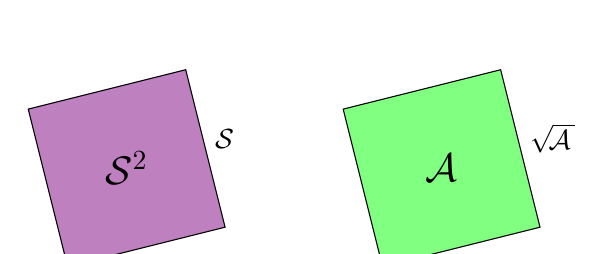
\begin{tikzpicture}[scale=0.5]
	\draw[fill=violet!50] (0,0) -- (4,1) -- (3,5) -- (-1,4) -- cycle;
	\draw (3.5,3.25) node[right]{$\mathcal{S}$};
	\draw (1.5, 2.5) node{\Large$\mathcal{S}^2$};
	\draw[fill=green!50] (8,0) -- (12,1) -- (11,5) -- (7,4) -- cycle;
	\draw (11.5,3.25) node[right]{$\sqrt{\!\mathcal{A}\,}$};
	\draw (9.5, 2.5) node{\Large$\mathcal{A}$};
\end{tikzpicture}\end{center}

Positive numbers have two square roots: one positive, one negative. Both 3 and $\umin3$ are square roots of 9, since $(3)(3) = 9$ and $(\umin3)(\umin3) = 9$. Zero is the only number that has exactly one square root: the square root of 0 is 0. Negative numbers cause some problems when it comes to square roots (stay tuned for more on that).

Most of the time, we'll be working with the positive square root of a number, called the \gls{principal square root} For example, the principal square root of 9 is 3 and the principal square root of 25 is 5.

The checkmark-ish symbol we use to denote the square root of $a$ is called the \gls{radical}: $\sqrt{a}$. This symbol means ``the principal square root of $a$''. So, $\sqrt{9} = 3$ and $\sqrt{25} = 5$. So, although $\umin3$ is a square root of 9, it is incorrect to write $\sqrt{9} = \umin3$ or $\sqrt{9} = \pm3$. This isn't quite rise to the level of \evilandwrong, but it's not right.\footnote{An algebra note from the future! When we simplify the expression $\sqrt{m^2}$, the result is $\abs{m}$, the absolute value of $m$. Do you see why? The value that comes out of the radical must be positive, because that notation gives the principal square root.}

When simplifying an expression or solving an equation, we won't always give both square roots.  A good guideline as we go along is to pay close attention and use the notation given in the problem. For example: \[\pm\sqrt{100} = \pm10 \qquad\text{and}\qquad -\sqrt{36} = \umin6\]
In these cases, the notation specifically indicates that we want both the positive and negative square root, or only the negative square root.

%%% Move to later, when solving equations?
%An Issue of Notation Now, squaring a number does something special. It gets rid of any negatives that may be attached to the number. So, when you square a number, you eliminate the sign. So, when you ``undo'' the square and take the square root, especially when solving an equation, you don't know if the original was positive or negative and you really get two solutions that actually work!
%
%Since you don't know which to give you give both. Of course when using square roots with the Pythagorean theorem, we ignore the negative root because distances aren't negative.
%
%So, if you choose to add the square root into a problem, you have to put the +/- in it. When you see it written in an expression, you are told which one you have. You need to remember this when you are simplifying a radical or solving an equation with a radical in it.

\subsection{Imaginary numbers}

Consider the expression $\sqrt{\umin16}$. This is a bit of a problem. We're meant to find the principal square root of $\umin16$, but the closest we can get is $4 \cdot \umin4 = \umin16$. It's true that $4$ and $\umin4$ have the same absolute value, but they're not the same number, which means we're not \textit{squaring} anything. So, there is no real number equal to $\sqrt{\umin16}$. Of course, $\umin16$ isn't special, the same argument applies to any negative number.

\begin{boxdef}[Square root of a negative number]
If $a < 0$, then there is no real number equal to $\sqrt{a}$.
\end{boxdef}

Note that this \textit{doesn't} mean that $\umin16$ doesn't have any square roots. It simply means that the square roots are not real numbers. The square roots of $\umin16$ are members of a set called the \textit{complex numbers} $\C$, but not members of the real numbers $\R$.

To build up the complex numbers, we introduce the so-called imaginary unit $\iu$ which has the property that $\iu^2 = −1$. Remember, the domain of Algebra 1 is the set real numbers. But, the domain of Algebra 2 and beyond is the set of complex numbers. So, if you're intrigued about imaginary numbers, just hang in there.

Our work in Algebra 1 will bring us mostly in contact with \textit{square roots}, but other roots are possible. For example a ``cube root'' of a number $a$ is a number $b$ such that $b\cdot b\cdot b = a$. We write $\sqrt[3]{a}$ to denote the cube root of $a$. Negative numbers under the cube root symbol are no problem: \[\sqrt[3]{\umin8} = \umin2 \qquad\text{since}\qquad \umin2\cdot\umin2\cdot\umin2 = \umin8\]


\subsection{(;,;) Irrationality of the square root of two}

We have shown that irrational numbers exist. Consider the mathematical argument below, which explains why the square root of 2 is irrational.

\textit{Step 1.~} Assume (for the moment) that $\sqrt{2}$ is, in fact, rational. In other words, that it can be written as the ratio of two integers. Then, we can write \[\sqrt{2} = \frac{a}{b}\] where $a$ and $b$ are relatively prime. That is to say, our fraction is in lowest terms.

\textit{Step 2.~} Square both sides of the equation above. \[2 = \frac{a^2}{b^2}\]

\textit{Step 3.~} Multiply both sides of this equation by $b^2$. \[2b^2 = a^2\] This means that $a^2$ is an even number. If $a^2$ is an even number, then $a$ must be an even number.

\textit{Step 4.~} If $a$ is an even number, then it is divisible by 2. In other words, there is an integer $m$ such that $a = 2m$.

\textit{Step 5.~} Substitute $2m$ for $a$ in the equation from Step 3, and simplify.\[\begin{aligned} 2b^2 &= (2m)^2 \\ 2b^2 &= 4m^2 \\ b^2 &= 2m^2 \end{aligned}\] This means that $b^2$ is an even number. If $b^2$ is an even number, then $b$ is an even number.

\textit{Step 6.~} If both $a$ and $b$ are even numbers, then the original fraction $\frac{a}{b}$ was not in lowest terms, which was our assumption! This contradiction shows that our original assumption cannot be true.

Thus, $\sqrt{2}$ cannot be written as a fraction. In other words, $\sqrt2$ is an irrational number.

\subsubsection{Thoughts to chew on}

Steps 3 and 5 both include assertions about numbers being even. How do we know when a number is even? Specifically, how do we know that $a^2$ and $b^2$ are even?

Steps 3 and 5 both go on to say something like ``if $a^2$ is even, then $a$ is even''. How do we know this is true? Under what circumstances will the square of a number be even or odd?

Step 6 argues that $\frac{a}{b}$ is not in lowest terms. How do we know this is true?

This is an example of \textit{proof by contradiction}. We assume that some statement is true, then show that this assumption leads to some kind of impossible situation. The impossibility means we have to reject the original assumption. What was our original assumption in this proof? What is the contradiction that results from that assumption?\footnote{Another famous proof by contradiction is Euclid's proof that there are infinitely many prime numbers. Have a look in \cref{app:primes}!}

% % % % % % % % % % % % % % % % % % % % % % % % % % % % % % % % % % % % % % % % 
\section{Simplified radical form}
\label{sec:radsimplifiedform}

%\begin{boxexplore}[TODO]
%TODO
%\end{boxexplore}
\addtodoitem{Startup exploration on simplified radical form?}

%When we take the square root of a perfect square we get an integer as the answer. It may come in handy to memorize the first 25 or so perfect squares, so that you can recognize them when they come up in a problem.

%\begin{center}
%\begin{tabular}{*{5}{C{0.15\textwidth}}}
%1^2 = 1	 &
%2^2 = 4	 &
%3^2 = 9	 &
%4^2 = 16 &
%5^2 = 25 \\
%6^2 = 36 &
%7^2 = 49 &
%8^2 = 64 &
%9^2 = 81 &
%10^2 = 100 \\
%11^2 = 121 &
%12^2 = 144 &
%13^2 = 169 &
%14^2 = 196 &
%15^2 = 225 \\
%16^2 = 256 &
%17^2 = 289 &
%18^2 = 324 &
%19^2 = 361 &
%20^2 = 400 \\
%21^2 = 441 &
%22^2 = 484 &
%23^2 = 529 &
%24^2 = 576 &
%25^2 = 625 \\
%\end{tabular}
%\end{center}

When we take the square root of a perfect square we get an integer as the answer. But, things are not so easy when taking the square root of a number that is not a perfect square. In fact, the square root of a non-square natural number will be an irrational number, like $\sqrt{2}$.

The \textit{exact value} of an irrational number can only be represented using some kind of symbol, like $\pi$ or $\sqrt2$. Writing out a decimal value -- no matter how many decimals you write down -- will always be an approximation. So, it's a good habit of mind to think ``should I be giving an exact answer to this problem, or is a decimal approximation good enough''. Very often, the context (or the directions) will make this choice clear.

To help us standardize the way we write radical expressions, we all agree to comply with \textit{simplified radical form}.

\begin{boxcrit}[Simplified radical form]
A radical expression is considered completely simplified if\ldots
\begin{enumerate}
\item Like radical terms have been combined.
\item The expression under the radical has no perfect square factors other than 1.
\item There are no fractions under the radical.
\item There are no radicals in the denominator of a fraction.
\end{enumerate}
\end{boxcrit}

Over the next few sections, we will discuss each of these criteria and the algebraic manipulations that we can use to make sure our expressions comply. The first criteria is quite straightforward, so let's get right to it.

\subsection{Like radical terms}

Criteria \#1 states that like radical terms must be combined. We combine radical terms as we do variable terms. For example, we are very familiar with the simplification \[x + x = 2x.\] We combine radical terms in exactly the same way: \[\sqrt5 + \sqrt5 = 2\cdot\sqrt5 = 2\sqrt5.\]
Note, in particular, that the sum here is not $\sqrt{10}$. Similarly, $3x + 4x = 7x$ and so with radicals, we have $3\sqrt{21} + 4\sqrt{21} = 7\sqrt{21}$. When we have a multiplication of a number times a radical, we can omit the multiplication symbol.

\addtodoitem{See Patty's alternative way of simplifying radicals.}

\begin{boxwarn}
When we say like radical terms ``can be combined'', don't go thinking you can add the numbers under the radical. To add the values like this is \evilandwrong.
\[ \sqrt{3} + \sqrt{3} \neq \sqrt{6}\]
Since a radical is like an exponent, this is the equivalent of saying $(a+b)^2=a^2+b^2$ which, by now, we know is not generally the case. You can't sprinkle that exponent across the sum!

While we're at it, don't get any ideas about splitting the radical-of-a-sum into the sum-of-radicals. This, too, is \evilandwrong.
\[\sqrt{2+14} \neq \sqrt{2} +\sqrt{14}\]
\end{boxwarn}


% % % % % % % % % % % % % % % % % % % % % % % % % % % % % % % % % % % % % % % % 
\subsection{Product properties of radicals}
%\label{sec:radproduct}

\begin{boxexplore}[Building blocks]
The number 1 is the \textit{additive building block} of the natural numbers. In other words: If we want to ``build'' any natural number using only addition, the only number we need is the number 1. Every natural number can be written as the sum of a bunch of 1's.

What are the \textit{multiplicative building blocks} of the natural numbers? Note that we have to say \textit{blocks} (plural) since the number 1 is not enough: multiplying together a bunch of 1's always gives us 1 as the product. What is the smallest collection of natural numbers that we need in order to build the rest using only multiplication?
\end{boxexplore}

The second criteria for simplified radical form states that the expression under the radical may have no perfect square factors other than 1. This may seem strangely worded. It clearly handles the idea that there should be no perfect squares under the radical, and that makes sense. Expressions like $\sqrt{4}$ and $\sqrt{25}$ can pretty obviously be simplified.

But, this criteria also catches expressions like $\sqrt{24}$ and $\sqrt{50}$ because those numbers, neither of which is a perfect square, each have a perfect square as a factor: 24 has 4 as a factor, and 50 has 25 as a factor.

How can we simplify an expression like $\sqrt{50}$ so that it has no perfect square factors under the radical? For help, we turn to:

\begin{boxdef}[Product rule of radicals]
For any $a \geq 0$ and $b \geq 0$, \[\sqrt{ab} = \sqrt{a} \cdot \sqrt{b}.\]

Note: In Algebra 1 we only use the square root version of this property, though in fact it applies to radicals of any degree: cube roots, fourth roots, and so on.
\end{boxdef}

This property looks an awful lot like the product rule for exponents, which makes sense since here we are undoing the power of a product rule, where the power is the exponent one-half!

\begin{boxex}
Express $\sqrt{50}$ in simplified radical form.

\exsoln\ We know $\sqrt{50}$ is not yet in simplified radical form because 50 is divisible by a perfect square, $50 = 25 \cdot 2$. We apply the multiplication property of radicals like so:
\[
\begin{aligned}
\sqrt{50} 	&= \sqrt{25 \cdot 2}
&& \quad \text{rewrite 50 to show its perfect square factor}\\
			&= \sqrt{25} \cdot \sqrt{2}
&& \quad \text{product rule of radicals}\\
			&= 5 \cdot \sqrt{2}
&& \quad \text{simplify the square root of a perfect square}
\end{aligned}
\]
So, $\sqrt{50} = 5\sqrt{2}$. These two expressions are equal, but only the second expression satisfies the criteria of simplified radical form.
\end{boxex}

\subsection{Different approaches to simplifying}

There are a number of ways to go about applying this property to simplify expressions. Use whatever approach makes the most sense to you! Here are some alternatives, though you might find a different approach that fits you better. In any case, it will probably be helpful to learn a variety of methods. Depending on the problem, some methods may be easier to use than others.

For example, let's examine different ways to get $\sqrt{108}$ into simplified radical form.

\subsubsection{Strategy 1: Largest square factor}

In this strategy, we find the largest perfect square factor and simplify it using the product rule for radicals. We might notice that $108 = 3 \times 36$: \[\sqrt{108} = \sqrt{36 \cdot 3} = \sqrt{36} \cdot \sqrt{3} = 6\sqrt{3}\]

\subsubsection{Strategy 2: One square at a time}

It might not be obvious what the largest perfect square is, so in this strategy we look for \textit{any} prefect square factor and work one square at a time. For instance, we might notice that 108 is divisible by 9 (how can we quickly spot divisibility by 9?). Then: \[\sqrt{108} = \sqrt{9 \cdot 12} = \sqrt{9} \cdot \sqrt{12} = 3 \cdot \sqrt{12} = 3 \cdot \sqrt{4 \cdot 3} = 3 \cdot \sqrt{4} \cdot \sqrt{3} = 3 \cdot 2 \cdot \sqrt{3} = 6\sqrt{3}\]

In this approach, we have to keep checking to see whether the number under the radical is ``square-free'' or not. After our first simplification, we have 12 under the radical. But 12 has 4 as a factor, so we have to do another simplification step.

This process might take a little longer, but it is sometimes easier to identify smaller perfect square factors and chip away at the problem, than it is to identify the largest perfect square factor and finish the problem in a single step.

\subsubsection{Strategy 3: Sniper method}

The idea here is to write the \textit{prime factorization} of the number under the radical, and then look for pairs of factors.\footnote{One way to break a number down into primes is using a factor tree. For a handy, if unusually-formatted, list of prime numbers, see \cref{app:primes}.} The factorization of $108 = 2 \cdot 2 \cdot 3 \cdot 3 \cdot 3$, so: \[\sqrt{108} = \sqrt{\underline{\color{blue}2 \cdot 2} \cdot \underline{\color{red}3 \cdot 3} \cdot 3} = \underline{\color{blue}2} \cdot \underline{\color{red}3} \cdot \sqrt{3} = 6\sqrt{3} \]

We've given this strategy the memorable (though perhaps gruesome) name \textit{the sniper method}. Think of the radical as a prison. There are snipers outside and any number that tries to escape needs to have a decoy. A single factor of 2 is stuck inside for life, but if the 2 has a partner (that is, if there's a $2 \cdot 2$ under the radical), then 2 can make a break for it!

But, only one of the partners survives the jailbreak. The snipers take out the decoy. In the example above, one 2 makes it out, and so does one 3. The final factor of 3 is partnerless, and left trapped inside its radical prison.

\begin{boxex}
	TO DO.
\end{boxex}

% % % % % % % % % % % % % % % % % % % % % % % % % % % % % % % % % % % % % % % % 
\subsection{Quotient properties of radicals}
\label{sec:radquotient}

Criteria \#3 and \#4 for simplified radical form are both pretty antiquated. They came about in the pre-calculator days when folks had to do a lot more calculation by hand and use large data tables to approximate radical values. Yet, these last two properties are still considered ``standard'' for simplified radical form.

\addtodoitem{Image of a sliderule?}

Rules were made to be broken, though, and there will be times when it's OK to break away from these criteria (\#4 especially). But we'll burn that bridge when we come to it. For now, all four criteria are in effect.

Both of these have to do with interactions between radicals and fractions. Criteria \#3 disallows fractions under the radical, and criteria \#4 forbids radicals in the denominator of a fraction.

To tackle Criteria \#3, for example when faced with expressions like \[\sqrt{\frac{4}{49}} \quad\text{or}\quad \sqrt{\frac{24}{25}}~,\]we turn to:

\begin{boxdef}[Quotient rule of radicals]
For any $a \geq 0$ and $b \geq 0$, \[\sqrt{\frac{a}{b}} = \dfrac{\sqrt{a}}{\sqrt{b}}.\]
\end{boxdef}

Again, this property applies to radicals of any degree (though for now we'll focus on square roots). And again, this property is just like the quotient rule for exponents, but with a rational exponent.

\begin{boxex}
Express $\sqrt{\frac{4}{49}}$ and $\sqrt{\frac{24}{25}}$ in simplified radical form.

\exsoln\ Here we have a fairly clear application of the rule:
\[\begin{aligned}
\sqrt{\frac{4}{49}}	&= \frac{\sqrt{4}}{\sqrt{49}}
&& \text{\quad quotient rule of radicals}\\[1ex]
&= \frac{2}{7}
&& \text{\quad simplify sqaure roots}\\
\end{aligned}
\]
In the second example, the numerator doesn't contain in a perfect square, so we must apply the product rule.
\[\begin{aligned}
\sqrt{\frac{24}{25}}	&= \frac{\sqrt{24}}{\sqrt{25}}
&& \text{\quad quotient rule of radicals}\\[1ex]
&= \frac{\sqrt{24}}{5}
&& \text{\quad simplify denominator}\\[1ex]
&= \frac{\sqrt{4\cdot6}}{5}
&& \text{\quad product rule in the numerator}\\[1ex]
&= \frac{\sqrt{4}\cdot\sqrt{6}}{5}\\[1ex]
&= \frac{2\sqrt{6}}{5}
\end{aligned}
\]
\end{boxex}

\subsection{Rationalizing the denominator}

When simplifying an expression using the division property, we may encounter something like the following: \[\sqrt{\frac{9}{2}} = \frac{\sqrt{9}}{\sqrt{2}} = \frac{3}{\sqrt{2}}\]
Back in the pre-calculator days, this led to criteria \#4, no radicals in the denominator of a fraction. After all, long division is bad enough to carry out by hand. Why not try to put yourself into a situation that makes division as easy and accurate as possible, and avoid dividing by a big ugly decimal?

When we have a radical in the denominator of a fraction we have an \textit{irrational denominator}. Our goal is to fix this by creating an equivalent fraction with a \textit{rational denominator}. The process of making this translation is called \gls{rationalizing the denominator}.

We will employ the trusty \textit{identity property of multiplication}. Remember, multiplying a number by a fancy 1 does not change the value of the number. The trick will be to choose the way our version of 1 looks. We are going to choose a fancy version of 1 that when multiplied by our irrational denominator gives us a rational number (in fact, an integer).

Study the following examples:

\begin{boxex}
Write $\dfrac{3}{\sqrt{2}}$ in simplified radical form.

\exsoln\ Note the clever use of multiplication by a fancy version of 1.
\[\begin{aligned}
\dfrac{3}{\sqrt{2}} &= \dfrac{3}{\sqrt{2}} \cdot 1
&&\quad\text{identity property of multiplication}\\
&= \dfrac{3}{\sqrt{2}} \cdot \dfrac{\sqrt{2}}{\sqrt{2}}
&&\quad\text{substitute a fancy version of 1}\\
&=~ \dfrac{3 \sqrt{2}}{\sqrt{2} \cdot \sqrt{2}}
&&\quad\text{multiply fractions}\\
&=~ \dfrac{3 \sqrt{2}}{2}
&&\quad\text{definition of square root (in the denominator)}\\
\end{aligned}
\]
\end{boxex}

Note that we chose as our fancy 1 \textit{exactly what we needed} to make the denominator of our fraction turn into an integer. This might seem like cheating, but it's a completely legal move, algebraically speaking.

Be sure to pay close attention. Sometimes we can use the division property in reverse to get rid of radicals in the denominator. We'll work the next example in two different ways to show the comparison.

\begin{boxex}
Write $\dfrac{\sqrt{84}}{\sqrt{6}}$ in simplified radical form.

\exsoln\ First, we'll rationalize the denominator using a fancy version of 1.
\[\begin{aligned}
\dfrac{\sqrt{84}}{\sqrt{6}} &= \dfrac{\sqrt{84}}{\sqrt{6}} \cdot 1
&&\quad\text{identity property of multiplication}
\\[1ex]
&= \dfrac{\sqrt{84}}{\sqrt{6}} \cdot \dfrac{\sqrt{6}}{\sqrt{6}}
&&\quad\text{substitute a fancy version of 1}
\\[1ex]
&=~ \dfrac{\sqrt{84} \cdot \sqrt{6}}{\sqrt{6} \cdot \sqrt{6}}
&&\quad\text{multiply fractions}
\\[1ex]
&=~ \dfrac{\sqrt{{\color{blue}84} \cdot {\color{red}6}}}{6}
&&\quad\text{product rule for radicals}
\\[1ex]
&=~ \dfrac{\sqrt{{\color{blue}2 \cdot 2 \cdot 3 \cdot 7} \cdot {\color{red}3 \cdot 2}}}{6}
&&\quad\text{simplify numerator using the sniper method}
\\[1ex]
&=~ \dfrac{2 \cdot 3 \sqrt{2 \cdot 7}}{6}
&&\quad\text{}
\\[1ex]
&=~ \dfrac{6 \sqrt{14}}{6}
&&\quad\text{}
\\[1ex]
&=~ \sqrt{14}
&&\quad\text{}\\
\end{aligned}
\]

Now, an alternative approach: We'll use the division property of radicals in reverse first, and then simplify the fraction under the radical.
\[\begin{aligned}
\dfrac{\sqrt{84}}{\sqrt{6}} &= \sqrt{\dfrac{84}{6}}
&&\quad\text{division property of radicals}
\\[1ex]
&=~ \sqrt{\dfrac{14}{1}}
&&\quad\text{simplify the fraction}
\\[1ex]
&=~ \sqrt{14}
&&\quad\text{Voil\`a.}
\end{aligned}
\]
\end{boxex}

The second approach is much easier in this case. It pays to work smart and do a bit of planning before charging ahead with an algorithm blindly. It may not always be this easy, though. Under what circumstances will we be able to use the kind of shortcut?

\begin{boxwarn}
Answers with fractions must be simplified, but folks sometimes get overly aggressive with the simplification. Consider the following: \[\frac{2}{\sqrt{6}} = \frac{2}{\sqrt{6}}\cdot\frac{\sqrt{6}}{\sqrt{6}} = \frac{2\sqrt{6}}{\sqrt{6}\cdot\sqrt{6}} = \frac{2\sqrt{6}}{6}\]
At this point, we can do one more simplification: \[\frac{2\sqrt{6}}{6} = \frac{\sqrt{6}}{3} \qquad \text{Yes!}\]
But we might be tempted to try and simplify even more: \[\frac{\sqrt{6}}{3} = \frac{\sqrt{2}}{1} \qquad \text{No!}\]
It's tempting, but we can't simplify using things \textit{under} the radical and things \textit{outside} the radical. That 6 under the radical cannot cancel with the 3 outside! To attempt such a simplification is \evilandwrong.
\end{boxwarn}

\begin{boxex}
Determine the value of $x$ given the equation: $2x^2+4x-3=40$.

\exsoln\ We'll use everything that we learned in \cref{ch:quadeq}! Our first step is to ensure that the first term is a perfect square, so we multiply through by 2.
\[4x^2 + 8x - 6 = 80\]
This also gives us an even linear coefficient, so it looks like we're ready for the quadrangle method.
\begin{center}
\quadrangle{2x}{2}{4x^2}{4x}{\color{red}4}
\end{center}
The quadrangle method predicts 4 as the constant term, but our equation has $-6$. APOE to the rescue:
\begin{align*}
4x^2 + 8x - 6 &= 80
\\
4x^2 + 8x + 4 &= 90
&&\text{APOE: add 10 to both sides}
\\
(2x+2)^2 &= 90
&&\text{based on the quadrangle diagram}
\\
2x+2 &= \pm\sqrt{90}
&&\text{square root of both sides}
\\
2x &= -2 \pm\sqrt{90}
&&\text{SPOE}
\\[1ex]
x &= \frac{-2 \pm\sqrt{90}}{2}
&&\text{DPOE}
\end{align*}
Almost there! Remember, we need to simplify our radicals! We can use the sniper method in this case:
\[\sqrt{90} = \sqrt{3\cdot3\cdot2\cdot5} = 3\sqrt{2\cdot5} = 3\sqrt{10}.\]
And so in the end, we have
\[\solset{\frac{-2 \pm 3\sqrt{10}}{2}}\]
We'll admit that these answers ain't pretty (note that there are two answers there!), but they are the values that satisfy our original quadratic equation.
\end{boxex}

% % % % % % % % % % % % % % % % % % % % % % % % % % % % % % % % % % % % % % % % 
\section{Coordinate geometry}
\label{sec:coordgeometry}

\begin{boxexplore}[Squarea]
As we saw in \cref{sec:radsquareroots}, a square with area $\mathcal{A}$ has side length $\sqrt{\!\mathcal{A}\,}$. Consider the figures below.

\begin{center}
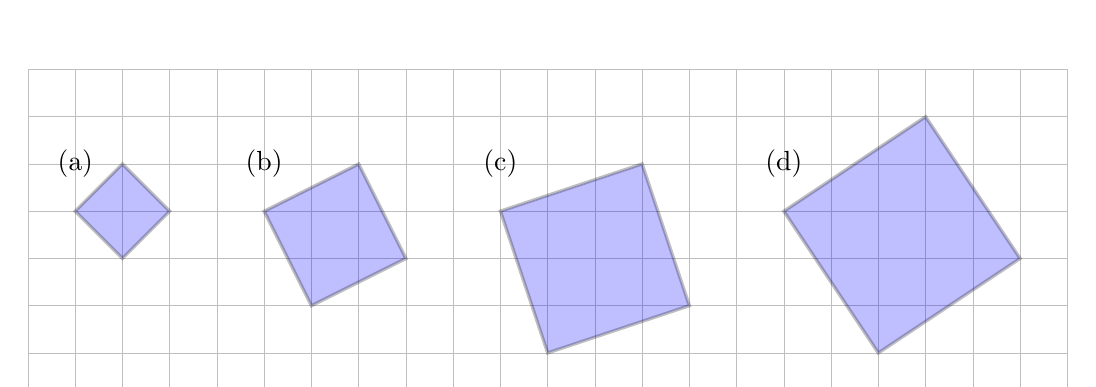
\begin{tikzpicture}[scale=0.6]
	\draw[black!25, very thin] (0,-1) grid (22,6);
	\draw(1,4) node{(a)};
	\draw[very thick, fill=blue, nearly transparent]
		(1,3) -- (2,2) -- (3,3) -- (2,4) -- cycle;
	\draw(5,4) node{(b)};
	\draw[very thick, fill=blue, nearly transparent]
		(5,3) -- (6,1) -- (8,2) -- (7,4) -- cycle;
	\draw(10,4) node{(c)};
	\draw[very thick, fill=blue, nearly transparent]
		(10,3) -- (11,0) -- (14,1) -- (13,4) -- cycle;
	\draw(16,4) node{(d)};
	\draw[very thick, fill=blue, nearly transparent]
		(16,3) -- (18,0) -- (21,2) -- (19,5) -- cycle;
\end{tikzpicture}
\end{center}

What is the area of each square? What is the side length of each square? Can you draw a square with side length $\sqrt{8}$? What about $\sqrt{13}$?

By the way, how do we know that each of these figures is, in fact, a square? (Hint: Think back to the slopes of parallel and perpendicular lines. What argument can we make for why the diagonal segments must be the same length in each figure?)
\end{boxexplore}

As an application of radicals and radical expressions, which are closely connected to the side lengths of squares, it's natural to discuss concepts from geometry. We'll begin with one of the most famous and important statements in mathematics.

\subsection{{P}ythagorean theorem}

It's a good bet that have seen the Pythagorean Theorem before, and that you will see it in every high school mathematics class you take, and many of the mathematics classed you take in college. In fact, the Pythagorean theorem is a foundational piece of an entire branch of mathematics based on the properties of triangles called \textit{trigonometry}.\footnote{Trigonometry begins with the study of triangles. \textit{Trigon} is another way of sayinga \textit{triangle} -- in fact it might be a better way of naming that shape! Most of the other polygons we know (pentagons, hexagons, octagons) have that \textit{-gon} suffix, and the prefix \textit{tri-} means ``three'' (as in tricycle).}

\begin{boxdef}[{P}ythagorean theorem]
The sum of the squares of the lengths of the \glspl{leg} of a right triangle is equal to the square of the length of the \gls{hypotenuse}.

In other words, if $a$ and $b$ represent the lengths of the legs (the perpendicular sides) of a right triangle, and $c$ represents the length of the hypotenuse (the longest side, opposite the right angle), then \[a^2 + b^2 = c^2.\]
\end{boxdef}

The theorem is named after Greek philosopher and mathematician Pythagoras of Samos, who lived around 570--495 BCE.\footnote{\addtodoitem{Need a good Pythagoras footnote.}} However, there is substantial evidence that the theorem was known to many different cultures from many different time periods. There is evidence, for instance, that the ancient Babylonians knew about Pythagorean triples (see the next section) more than 1000 years BCE.

Let's jump in with a famous right triangle: one with legs of length 3 and 4, and with hypotenuse of length 5. If we draw squares on the sides of the triangle, we can see that the sums of the areas of the two smaller squares (9+16) is exactly equal to the area of the largest square (25).
\begin{center}
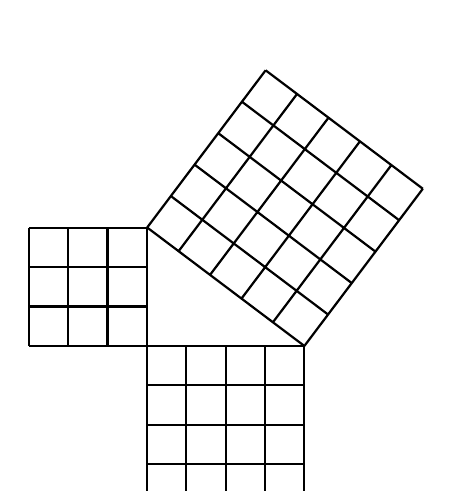
\begin{tikzpicture}[xscale=0.5,yscale=0.5]
	%% grid setup
	%\draw[very thin,color=gray!25] (0,0) grid (12,13);
	\draw[thick] (1,5) grid (4,8);
	\draw[thick] (4,1) grid (8,5);
	\draw[thick,rotate around={53:(8,5)}] (8,5) grid (13,10);
\end{tikzpicture}
\end{center}

This relationship holds true for all right triangles as does its \textit{converse}. The converse of the theorem states that if we have three numbers that satisfy the Pythagorean theorem, then we know that they must form the sides of a right triangle.

You might be asking yourself, ``How do we know that the theorem is true for \textit{every right triangle ever}?'' Those who are curious might enjoy exploring this question at the end of this section.

\subsection{{P}ythagorean triples}

\begin{boxdef}[{P}ythagorean triple]
A \textit{Pythagorean triple} is a set of three positive integers satisfying the Pythagorean theorem.
\end{boxdef}

There are infinitely many Pythagorean triples, and it is quite handy to know a few by heart. (This is because they are used quite a bit in problems, and those delightful standardized tests we all know and love.) Here are a few common Pythagorean triples:
\[
(3, 4, 5) \qquad\qquad
(5, 12, 13) \qquad\qquad
(7, 24, 25) \qquad\qquad
(9, 40, 41) \qquad\qquad
(8, 15, 17)
\]
The benefit of memorizing a few of these is that, if you see that a right triangle that has leg lengths of 7 and 24, you know that the hypotenuse has length 25 without having to do any calculations.

The triples above are called \inlinedef{primitive Pythagorean triples} because the three values are relatively prime. You can generate new Pythagorean triples by scaling up a triple that you know. For example $(6, 8, 10)$ is a triple formed by scaling up the $(3, 4, 5)$ triple by a factor of 2.

\subsubsection{Find-the-missing-side problems}

The classic application of the Pythagorean theorem is to find a missing side length, either a leg or a hypotenuse, and you may have solved problems like this before. Now that we have some algebra skills, however, our answers should be given in simplified radical form! No more decimal approximations (unless the directions state otherwise)!

\begin{boxex}
Find the length of the digaonal of a 4-by-8 rectangle.

\exsoln\ This problem might not, at first, seem to have anything to do with the Pythagorean theorem. The theorem, after all, is about right triangles, and this question is about a rectangle! Drawing a picture helps to reveal the connection:

\begin{center}\begin{tikzpicture}[scale=0.5]
	\draw[dashed] (0,0) -- (8,4);
	\draw (0,0) rectangle (8,4);
	\draw (4,0) node[below]{8};
	\draw (8,2) node[right]{4};
	\draw (4, 2) node[above]{$d$};
\end{tikzpicture}\end{center}

If we let $d$ represent the length of the diagonal, then we can see that it is the hypotenuse of a right triangle with legs of length 4 and 8. So:
\begin{align*}
d^2	&= 4^2 + 8^2
&&\quad\text{Pythagorean theorem}\\
d^2&= 16 + 64\\
d^2&= 80\\
d 	&= \sqrt{80}
&&\quad\text{square root of both sides}\\
d 	&= \sqrt{2 \cdot 2 \cdot 2 \cdot 2 \cdot 5}
&&\quad\text{simplify using the sniper method}\\
d 	&= 2 \cdot 2 \cdot \sqrt{5}\\
d 	&= 4\sqrt{5}
\end{align*}
So, a 4-by-8 rectangle has a diagonal which is $4\sqrt5$ units long.
\end{boxex}

To get a feel for whether this answer is reasonable, we could find a decimal approximation using a calculator (it's about 9 units long, which seems OK), or we could reason as follows. We know that $\sqrt{4} = 2$, and so $\sqrt{5}$ must be a bit more than 2. So, $4\sqrt{5}$ must be a bit more than 8. This seems reasonable.

On the other hand, if we had gotten $4\sqrt{8}$ we might reason that $\sqrt{9} = 3$ and so $4\sqrt{8}$ must be a bit less than $4\sqrt{9} = 4\cdot3 = 12$. This is too long for the diagonal of a 4-by-8 rectangle, since the two sides together are only 12 units long in total!

\subsection{Distance formula}

\begin{boxexplore}[Grid distance]
Find the length of the line segment connecting the points $(1,2)$ and $(6,7)$.
\end{boxexplore}

One important application of the Pythagorean theorem is called the \gls{distance formula}. It is a formula that we can use to calculate the distance between two points on a coordinate grid. In the startup exploration, we have the segment pictured below:

\begin{center}
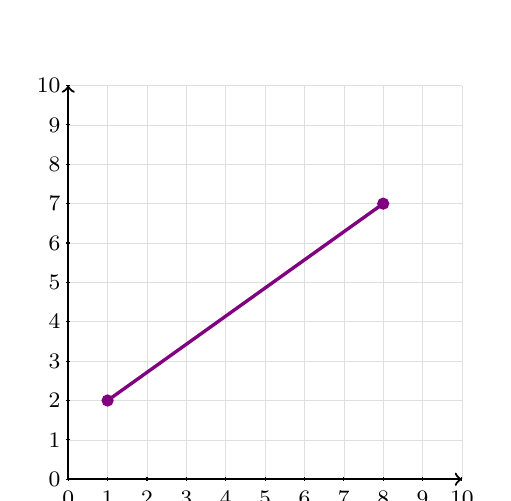
\begin{tikzpicture}[xscale=0.5,yscale=0.5]
	%% grid setup
	\draw[very thin, color=gray!25] (0,0) grid (10,10);
	\draw[->,thick] (0,0) -- (10,0); % node[right] {$x$};
	\draw[->,thick] (0,0) -- (0,10); % node[above] {$y$};
	\foreach \x in {0,...,10} \draw (\x,0.05) -- (\x,-0.05) node[below] {\footnotesize\x};
	\foreach \y in {0,...,10} \draw (-0.05,\y) -- (0.05,\y) node[left] {\footnotesize\y};
	\draw[very thick,violet] (1,2) -- (8,7); % node[right] {$x$};
	\draw[violet] plot[only marks,mark=*,mark size=4] coordinates{(1,2)(8,7)};
\end{tikzpicture}
\end{center}

If we think of the line segment into the hypotenuse of a right triangle, then we can use the Pythagorean theorem! The legs are the vertical and horizontal distances between the points, as in a slope triangle.

Draw the triangle, find the horizontal and vertical distances, then apply the Pythagorean theorem.

\begin{center}
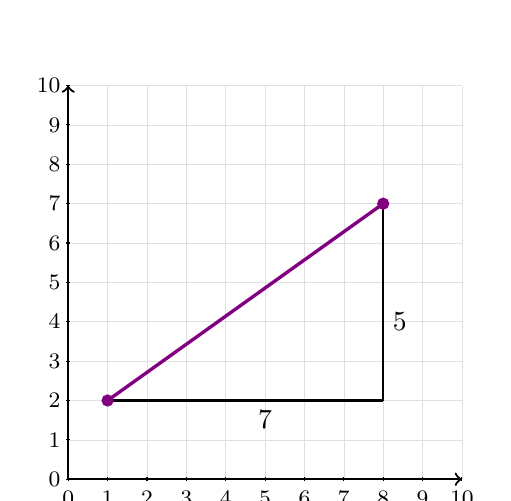
\begin{tikzpicture}[xscale=0.5,yscale=0.5]
	%% grid setup
	\draw[very thin, color=gray!25] (0,0) grid (10,10);
	\draw[->,thick] (0,0) -- (10,0); % node[right] {$x$};
	\draw[->,thick] (0,0) -- (0,10); % node[above] {$y$};
	\foreach \x in {0,...,10} \draw (\x,0.05) -- (\x,-0.05) node[below] {\footnotesize\x};
	\foreach \y in {0,...,10} \draw (-0.05,\y) -- (0.05,\y) node[left] {\footnotesize\y};
	\draw[very thick,violet] (1,2) -- (8,7); % node[right] {$x$};
	\draw[thick] (1,2) -- (8,2);
	\draw (5,2) node[below] {7};
	\draw[thick] (8,2) -- (8,7);
	\draw (8,4) node[right] {5};
	\draw[violet] plot[only marks,mark=*,mark size=4] coordinates{(1,2)(8,7)};
\end{tikzpicture}
\end{center}

The horizontal distance is 7 units, and the vertical distance is 5 units. Those are the legs of the right triangle. Then, we use the theorem to find the length of the hypotenuse: \[\begin{aligned} a^2 + b^2 &= c^2 \\ 5^2 + 7^2 &= c^2 \\ 25 + 49 &= c^2 \\ 74 &= c^2 \\ \sqrt{74} &= c\end{aligned}\]

Since the process is the same every time, we can generalize to find the distance between any two points $(x_1, y_1)$ and $(x_2, y_2)$ in the plane.

\begin{center}
\begin{tikzpicture}[xscale=0.5,yscale=0.5]
	%% grid setup
%	\draw[very thin, color=gray!25] (0,0) grid (10,10);
	\draw[->,thick] (0,0) -- (10,0); % node[right] {$x$};
	\draw[->,thick] (0,0) -- (0,10); % node[above] {$y$};
%	\foreach \x in {0,...,10} \draw (\x,0.05) -- (\x,-0.05) node[below] {\footnotesize\x};
%	\foreach \y in {0,...,10} \draw (-0.05,\y) -- (0.05,\y) node[left] {\footnotesize\y};
	%% line segment
	\draw[very thick,blue] (2,3) -- (8,7); % node[right] {$x$};
	%% horizontal labels
	\draw[dotted] (2,3) -- (2,0);
	\draw (2,0.1) -- (2,-0.1) node[below]{$x_1$};
	\draw[dotted] (8,7) -- (8,0);
	\draw (8,0.1) -- (8,-0.1) node[below]{$x_2$};
	%% vertical labels
	\draw[dotted] (2,3) -- (0,3);
	\draw (0.1,3) -- (-0.1,3) node[left]{$y_1$};
	\draw[dotted] (8,7) -- (0,7);
	\draw (0.1,7) -- (-0.1,7) node[left]{$y_2$};

%	\draw (1,2) node[below]{$(x_1, y_1)$};
%	\draw[thick] (1,2) -- (8,2);
%	\draw (5,2) node[below] {$x_2 - x_1$};
%	\draw[thick] (8,2) -- (8,7);
%	\draw (8,4) node[right] {$y_2 - y_1$};
	\draw[blue] plot[only marks,mark=*,mark size=4] coordinates{(2,3)(8,7)};
\end{tikzpicture}
\end{center}

\begin{boxdef}[Distance formula]
Given two points in the plane $(x_1, y_1)$ and $(x_2, y_2)$, the length $d$ of the line segment connecting the points is given by the formula:
\[d = \sqrt{ (x_2 - x_1)^2 + (y_2 - y_1)^2 }.\]
\end{boxdef}

This might look like a bunch of alphabet soup, much harder to remember than the Pythagorean theorem. But remember: this \textit{is} the Pythagorem theorem! If you forget the formula, don't panic! Just remember that the line segment between the two points is the hypotenuse of a right triangle.

\begin{boxex}
Find the distance between the points $(5, 12)$ and $(-4, -2)$.

\exsoln\ We will use the distance formula, but note that we have both subtraction and negative numbers. Watch those minus signs!
\[\begin{aligned}
d &= \sqrt{ (5 - \umin4)^2 + (12 - \umin2)^2 } \\
&= \sqrt{ 9^2 + 14^2 } \\
&=\sqrt{ 81 + 196 } \\
&=\sqrt{ 277 }
\end{aligned}\]
Since 277 is prime, we know our answer complies with simplified radical form, so we're all done. The distance betnwee the two points is $\sqrt{277}$ units.
\end{boxex}

\subsection{Midpoint formula}

When working with the distance formula, there is a related formula for finding the coordinates of \textit{midpoint} of a given line segment. Suppose we wanted to find the midpoint of the line segment connecting $(2,8)$ and $(8,4)$.
\begin{center}
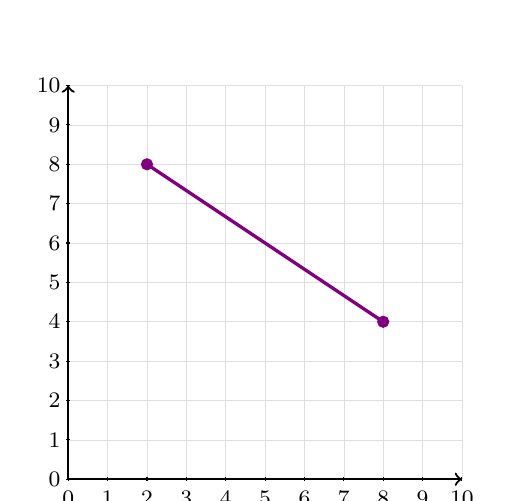
\begin{tikzpicture}[xscale=0.5,yscale=0.5]
	%% grid setup
	\draw[very thin, color=gray!25] (0,0) grid (10,10);
	\draw[->,thick] (0,0) -- (10,0); % node[right] {$x$};
	\draw[->,thick] (0,0) -- (0,10); % node[above] {$y$};
	\foreach \x in {0,...,10} \draw (\x,0.05) -- (\x,-0.05) node[below] {\footnotesize\x};
	\foreach \y in {0,...,10} \draw (-0.05,\y) -- (0.05,\y) node[left] {\footnotesize\y};
	\draw[very thick,violet] (2,8) -- (8,4); % node[right] {$x$};
	\draw[violet] plot[only marks,mark=*,mark size=4] coordinates{(2,8)(8,4)};
\end{tikzpicture}
\end{center}
Well, it sure looks like the midpoint of this segment is the point $(5,6)$\ldots\ but can we be sure?

One way to explain this is by drawing in the right triangle, and then chopping that triangle into four congruent sub-triangles. (Remember our work with the Sierpi\'{n}ski triangle ages ago?)
\begin{center}
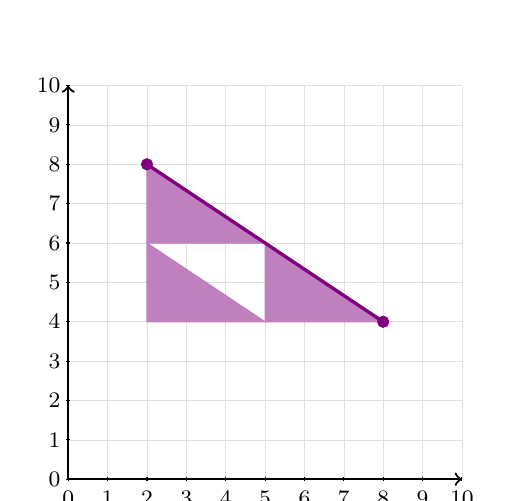
\begin{tikzpicture}[xscale=0.5,yscale=0.5]
	%% grid setup
	\draw[very thin, color=gray!25] (0,0) grid (10,10);
	\draw[->,thick] (0,0) -- (10,0); % node[right] {$x$};
	\draw[->,thick] (0,0) -- (0,10); % node[above] {$y$};
	\foreach \x in {0,...,10} \draw (\x,0.05) -- (\x,-0.05) node[below] {\footnotesize\x};
	\foreach \y in {0,...,10} \draw (-0.05,\y) -- (0.05,\y) node[left] {\footnotesize\y};
	\draw[violet!50, fill=violet!50] (2,8)--(2,6)--(5,6)--cycle;
	\draw[violet!50, fill=violet!50] (2,6)--(2,4)--(5,4)--cycle;
	\draw[violet!50, fill=violet!50] (5,6)--(5,4)--(8,4)--cycle;
	\draw[very thick,violet] (2,8) -- (8,4); % node[right] {$x$};
	\draw[violet] plot[only marks,mark=*,mark size=4] coordinates{(2,8)(8,4)};
\end{tikzpicture}
\end{center}
This diagram suggests that the $x$-coordinate of the midpoint of the hypotenuse is exactly halfway between the $x$-coordinates of the legs. The same goes for the $y$-coordinate. So, to find the coordinates of the midpoint, all we have to do is average the coordinates of the endpoints! Once again, you don't have to memorize this formula if you remember where it comes from!


\begin{boxdef}[Midpoint formula]
Given a line segment with endpoints $(x_1, y_1)$ and $(x_2, y_2)$, the coordinates of the midpoint of the segment are \[\left( \frac{x_1+x_2}{2} ~,~ \frac{y_1+y_2}{2} \right)\]
\end{boxdef}

\begin{boxex}
Find the midpoint of the segment connecting the points $(-13,8)$ and $(6, -2)$.

\inlineex{Solution:} Let's calculate the midpont first, and then check our answer by drawing a picture. The formula is pretty straightforward. The midpoint should be located at: \[\left( \frac{-13+6}{2} ~,~ \frac{8+\umin2}{2} \right) = \left( \frac{-7}{2} ~,~ \frac{6}{2} \right) = (-3.5, 3) \]
Here's a graph to check that our answer is reasonable:
\begin{center}
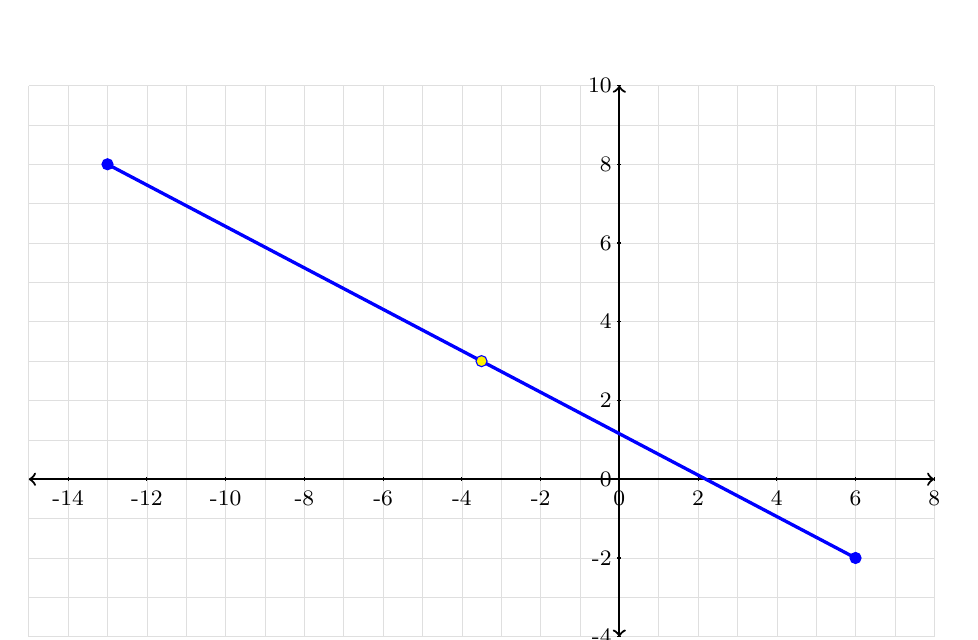
\begin{tikzpicture}[scale=0.5]
	%% grid setup
	\draw[very thin, color=gray!25] (-15,-4) grid (8, 10);
	\draw[<->,thick] (-15,0) -- (8,0);
	\draw[<->,thick] (0,-4) -- (0,10);
	\foreach \x in {-14,-12,...,8} \draw (\x,0.05) -- (\x,-0.05) node[below] {\footnotesize\x};
	\foreach \y in {-4,-2,...,10} \draw (-0.05,\y) -- (0.05,\y) node[left] {\footnotesize\y};
	%% line segment
	\draw[very thick,blue] (-13,8)--(6,-2);
	\draw[blue] plot[only marks,mark=*,mark size=4] coordinates{(-13,8)(6,-2)};
	\draw[blue, fill=yellow] plot[only marks,mark=*,mark size=4] coordinates{(-3.5,3)};
\end{tikzpicture}
\end{center}
\end{boxex}

\subsection{(;,;) Proof of the {P}ythagorean theorem}
\label{sec:pythagproof}

Imagine a pizza box and four identical slices of pizza\ldots\ where the pizza slices are right triangles. (Not typical for pizza slices, we know, but go with it.)

\begin{center}
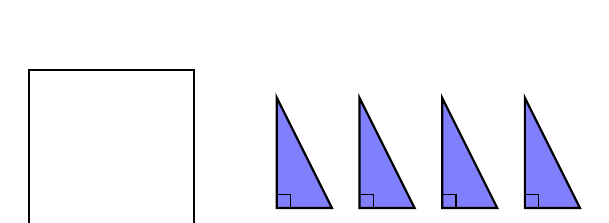
\begin{tikzpicture}[scale=0.35]
	\draw[thick] (0,0) rectangle (6,6);
	\foreach \x in {9,12,15,18} {
		\draw[thick, fill=blue!50] (\x,1) -- (\x+2,1) -- (\x,5) -- cycle;
		\draw (\x,1) rectangle (\x+0.5, 1.5);
	}
\end{tikzpicture}
\end{center}

Consider two different arrangements of the same four pizza slices inside the same pizza box. The slices are arranged to that they fit inside without overlapping, and they lay flat on the bottom of the box.

\begin{center}
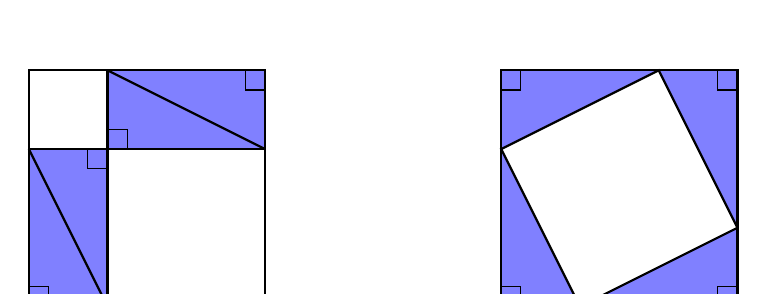
\begin{tikzpicture}[scale=0.5]
	%% Box 1
	\draw[thick] (0,0) rectangle (6,6);
	\draw[thick,fill=blue!50] (0,0) rectangle (2,4);
	\draw[thick,fill=blue!50] (2,4) rectangle (6,6);
	\draw (0,0) rectangle (0.5, 0.5);
	\draw (2,4) rectangle (1.5, 3.5);
	\draw (2,4) rectangle (2.5, 4.5);
	\draw (6,6) rectangle (5.5, 5.5);
	\draw[thick] (0,4) -- (2,0);
	\draw[thick] (2,6) -- (6,4);
	%% Box 2
	\begin{scope}[xshift=12cm]
	\draw[thick,fill=blue!50] (0,0) rectangle (6,6);
	\draw (0,0) rectangle (0.5, 0.5);
	\draw (0,6) rectangle (0.5, 5.5);
	\draw (6,0) rectangle (5.5, 0.5);
	\draw (6,6) rectangle (5.5, 5.5);
	\draw[thick,fill=white] (0,4) -- (2,0) -- (6,2) -- (4,6) -- cycle;
	\end{scope}
\end{tikzpicture}
\end{center}

\textit{Step 1:~} Consider the image on the left: Write an expression for the area of the box that is left \textit{uncovered}. You may find it helpful to label the sides of the triangles, or the sides of the box (or both).

You may be tempted to say that the uncovered regions are squares. How do we know -- for sure -- that these two regions are actually \textit{squares}, as opposed to some other quadrilateral?

\textit{Step 2:~} Consider the image on the right: Write an expression for the area of the box that is left \textit{uncovered}. Use the same labels you assigned when studying the other picture.

Again, you may be tempted to say that the uncovered region is a square. How do we know that it is a square (and not, say, a rhombus)?

\textit{Step 3:~} The area that is uncovered by the pizza slices is the same. (How do we know this?) What does this tell us about the two expressions for the uncovered area?

\subsubsection{Alternative approach}

In fact, we can explain the theorem using only the right-hand diagram. Let $a$ and $b$ be the lengths of the legs of one of the triangles, and let $c$ be the length of the hypotenuse.

\begin{center}
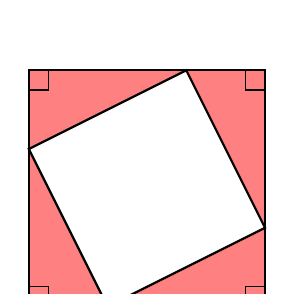
\begin{tikzpicture}[scale=0.5]
	%% Box 2
	\draw[thick,fill=red!50] (0,0) rectangle (6,6);
	\draw (0,0) rectangle (0.5, 0.5);
	\draw (0,6) rectangle (0.5, 5.5);
	\draw (6,0) rectangle (5.5, 0.5);
	\draw (6,6) rectangle (5.5, 5.5);
	\draw[thick,fill=white] (0,4) -- (2,0) -- (6,2) -- (4,6) -- cycle;
\end{tikzpicture}
\end{center}

\textit{Step 1:~} Express the sides of the largest square (the pizza box itself) in terms of $a$ and $b$.

\textit{Step 2:~} Express the area of the largest square in terms of $a$ and $b$. (Hint: You'll need the sum to a power rule.)

\textit{Step 3:~} The area of the largest square can also be expressed at the sum of the areas of the four triangles plus the area of the tiled square. Express the area of the largest square in this way (in terms of $a$, $b$, and $c$).

\textit{Step 4:~} We now have two ways of expressing the area of the largest square. What happens when set them equal to each other?

\subsubsection{Generalizing}

All the figures in this discussion have been drawn using a particular square and a particular triangle. Explain why these arguments are proof that the Pythagorean theorem is true for any right triangle, not just the specific triangle that is pictured in these diagrams.


% % % % % % % % % % % % % % % % % % % % % % % % % % % % % % % % % % % % % % % % 
\chaptersummary

Our algebra toolbox grows ever larger! We can now handle the simplification of numerical expressions that include square roots. This, combined with our work from the previous chapter, means that we can handle even the most ``impolite'' of quadratic equations. Plus, along the way we have discovered some fundamental results from geometry.

These skills are valuable, without a doubt, but we haven't looked closely at quadratic functions in detail. These are the focus of the next chapter. Onward!

\chaptercopyright

%%%%\include{ch14_quadfunc}
%%%%\include{ch15_polynomials}
%%%%\include{ch16_factoring}
%%%
%%%% Appendices
%%%\appendix
%%%\newcounter{primeHctr}
%%%\include{appA_primes}
%%%
%%%% % % % % % % % % % % % % % % % % % % % % % % % % % % % % % % % % % % % % % % % 
%%%% 
%%%% BACK MATTER
%%%%
%%%\backmatter
%%%\pagestyle{plain}
%%%
%%%%
% Back matter for the Algebranomicon
%

%\chapter{Back Matter}
%Glossary, bibliography, and index removed during editing process.

\cleardoublepage
\phantomsection
\addcontentsline{toc}{chapter}{Glossary}
%\glossarystyle{listhypergroup}
\glsaddall
\printglossaries

\cleardoublepage
\phantomsection
\addcontentsline{toc}{chapter}{Bibliography}
\bibliographystyle{plain}
\nocite{*} %%% include all references, even those not cited
\bibliography{algbookrefs}

\cleardoublepage
\phantomsection
\addcontentsline{toc}{chapter}{Index}
\printindex

%%%
%%%\clearpage
%%%
%%%% Close output stream for to-do list
%%%\immediate\closeout\outputstream
%%%
%%%\end{document}


%
% Partial inclusion, for piecewise development
%
%\includeonly{ch08_systems}

%%%
%%%\usepackage{floatrow}			% this automatically centers all floats
%%%\floatplacement{table}{hbtp}		% all tables are given the [hbtp] option
%%%\floatplacement{figure}{hbtp}	% all figures are given the [hbtp] option
%%%
%%%\usepackage{wallpaper}			% to tile background image on cover page
%%%
%%%% % % % % % % % % % % % % % % % % % % % % % % % % % % % % % % % % % % % % % % % 
%%%
%%%% Custom table commands
%%%\usepackage{jermer_tables}
%%%
%%%% Custom mathematics commands
%%%\usepackage{jermer_math}
%%%
%%%% Environment for formatting commented work
%%%\usepackage{algnom_commwork}
%%%
%%%% % % % % % % % % % % % % % % % % % % % % % % % % % % % % % % % % % % % % % % % 
%%%%
%%%% Callout boxes
%%%%
%%%\usepackage{algnom_boxes}
%%%
%%%% Enable formatting for one-line examples
%%%\usepackage{enumitem}
%%%
%%%% % % % % % % % % % % % % % % % % % % % % % % % % % % % % % % % % % % % % % % % 
%%%%
%%%% Graphs
%%%%
%%%\usepackage{algnom_graphs}
%%%
%%%% Enable fractal drawing
%%%\usepackage{tikz}
%%%\usetikzlibrary{patterns}
%%%\usetikzlibrary{decorations.fractals}
%%%\usetikzlibrary{lindenmayersystems}
%%%
%%%\usepackage[autoplay, loop]{animate}
%%%
%%%% % % % % % % % % % % % % % % % % % % % % % % % % % % % % % % % % % % % % % % % 
%%%%
%%%% Font selection
%%%%
%%%\RequirePackage[T1]{fontenc}
%%%\RequirePackage{cmbright}
%%%
%%%% Special inline formatting for the name ''Algebranomicon'
%%%\newcommand{\algebranomicon}{\textcolor{black}{$\mathfrak{Algebranomicon}$}}
%%%
%%%% Special inline formatting for calculator commands
%%%\newcommand{\calculator}[1]{\texttt{#1}}
%%%
%%%% % % % % % % % % % % % % % % % % % % % % % % % % % % % % % % % % % % % % % % % 
%%%%
%%%% Page layout, margins, line spacing
%%%%
%%%\usepackage[letterpaper, margin=1in]{geometry}
%%%
%%%% Set line spacing to 1.5
%%%\usepackage{setspace}
%%%\onehalfspacing
%%%
%%%% At paragraph break use blank line w/ no indentation 
%%%\usepackage{parskip}
%%%
%%%% Restore the paragraph skip length inside minipages
%%%\setlength{\parskip}{\bigskipamount}
%%%\makeatletter
%%%	\newcommand{\@minipagerestore}{\setlength{\parskip}{\medskipamount}}
%%%\makeatother
%%%
%%%% Enable custom page headers and footers
%%%\usepackage{fancyhdr}
%%%\setlength{\headheight}{15pt}
%%%
%%%% % % % % % % % % % % % % % % % % % % % % % % % % % % % % % % % % % % % % % % % 
%%%%
%%%% Formatting chapter and section titles
%%%%
%%%\usepackage{titlesec}
%%%
%%%% Start sections on a new page, except for the first section of a new chapter
%%%\usepackage{etoolbox}
%%%\newtoggle{afterpart}
%%%\pretocmd{\section}
%%%{
%%%	\iftoggle{afterpart}
%%%	{\global\togglefalse{afterpart}}	% we're after a part
%%%	{\clearpage}						% we're not immediately after a part
%%%}{}{}
%%%\pretocmd{\chapter}
%%%{
%%%	\clearpage						% do a page break
%%%	\global\toggletrue{afterpart}		% tell \section we're just after a part
%%%}{}{}
%%%
%%%% Draw horizontal rule under section titles
%%%\newcommand{\trule}{\color{black!25}\titlerule[1pt]}
%%%
%%%\titleformat{\section}
%%%	{\normalfont\bfseries\Large}
%%%	{\thesection}{1em}{}[\trule]
%%%
%%%% Enable fancy formatting for chapter quotes
%%%\usepackage{epigraph}
%%%
%%%% Command to wrap epigraph commands.
%%%% Usage: \chapquote{quote}{author}
%%%\newcommand{\chapquote}[2]{
%%%	\epigraphhead[50]{\epigraph{#1}{\textit{#2}}}
%%%}
%%%
%%%% Adjust epigraph rule color
%%%\makeatletter
%%%\renewcommand{\@epirule}
%%%	{\color{black!25}\rule[.5ex]{\epigraphwidth}{\epigraphrule}}
%%%\makeatother
%%%
%%%% Command for consistent formatting of "chapter summary" section
%%%\newcommand{\chaptersummary}{\subsection*{>> Chapter summary <<}}
%%%
%%%% % % % % % % % % % % % % % % % % % % % % % % % % % % % % % % % % % % % % % % % 
%%%%
%%%% Footnotes
%%%%
%%%\usepackage[hang,bottom]{footmisc}
%%%
%%%% Footnote hanging indent
%%%\setlength{\footnotemargin}{1em}
%%%
%%%% Space between two footnotes
%%%\setlength{\footnotesep}{3ex}
%%%
%%%% Space between text and notes -- Note sure if this is needed?
%%%\setlength{\skip\footins}{5ex}
%%%
%%%% % % % % % % % % % % % % % % % % % % % % % % % % % % % % % % % % % % % % % % % 
%%%%
%%%% Cross references
%%%%
%%%\usepackage[hidelinks]{hyperref}
%%%
%%%% Formatting hyperlinks
%%%%\usepackage{hyperref}
%%%%\hypersetup{
%%%%	colorlinks   = true,	%Colours links instead of ugly boxes
%%%%	urlcolor     = blue,	%Colour for external hyperlinks
%%%%	linkcolor    = blue,	%Colour of internal links
%%%%	citecolor   = red		%Colour of citations
%%%%}
%%%
%%%\usepackage{cleveref}
%%%\providecommand\phantomsection{}
%%%
%%%% Custom labels for clever references to "examples"
%%%\crefname{counterExample}{example}{examples}
%%%\Crefname{counterExample}{Example}{Examples}
%%%
%%%% % % % % % % % % % % % % % % % % % % % % % % % % % % % % % % % % % % % % % % % 
%%%%
%%%% Glossary and index
%%%%
%%%% Enable glossary creation
%%%\usepackage[nonumberlist, nopostdot]{glossaries}
%%%\setglossarystyle{listhypergroup}
%%%\renewcommand*{\glshypernavsep}{ $\cdot$ }
%%%\makeglossaries
%%%
%%%% Enable index creation
%%%\usepackage{makeidx}
%%%\makeindex
%%%
%%%% Commands to create simultaneous glossary-index entries
%%%% Good idea? Bad idea?
%%%\let\oldgls\gls
%%%\renewcommand*{\gls}[1]{\inlinedef{\oldgls{#1}}\index{#1}}
%%%
%%%\let\oldGls\Gls
%%%\renewcommand*{\Gls}[1]{\inlinedef{\oldGls{#1}}\index{#1}}
%%%
%%%\let\oldglspl\glspl
%%%\renewcommand*{\glspl}[1]{\inlinedef{\oldglspl{#1}}\index{#1}}
%%%
%%%\let\oldGlspl\Glspl
%%%\renewcommand*{\Glspl}[1]{\inlinedef{\oldGlspl{#1}}\index{#1}}
%%%
%%%% % % % % % % % % % % % % % % % % % % % % % % % % % % % % % % % % % % % % % % % 
%%%%
%%%% To-do lists
%%%%
%%%\newcommand{\addtodoitem}[1]
%%%{%
%%%	% Add item to the file 'todolist.txt'
%%%	\immediate\write\outputstream{[TODO] Section \thesection. #1}
%%%}
%%%
%%%\newcommand{\kverse}[1]
%%%{%
%%%	% Add item to the file 'todolist.txt'
%%%	\immediate\write\outputstream{[Krumbliverse] Section \thesection. #1}
%%%}

\newcommand{\chaptercopyright}
{
\ifdefined\indchap

\clearpage
\thispagestyle{empty}
\addtocounter{page}{-1} 

\begingroup
\urlstyle{same}

\null\vfill
\begin{center}
\begin{minipage}{0.75\textwidth}

This document (generated \today) is an excerpt from The Algebranomicon by Patty C. Hill and Jason L. Ermer.

The Algebranomicon is copyright \copyright\ 2014 by Patty C. Hill and Jason L. Ermer, and made available under a \href{http://creativecommons.org/licenses/by-sa/4.0/}{Creative Commons Attribution-ShareAlike 4.0 International License}.

For more information visit \href{http://www.algebranomicon.org}{www.Algebranomicon.org}.
\end{minipage}
\end{center}
\vfill\null

\endgroup
\clearpage

\else
\fi
}

% % % % % % % % % % % % % % % % % % % % % % % % % % % % % % % % % % % % % % % % 
% % % % % % % % % % % % % % % % % % % % % % % % % % % % % % % % % % % % % % % % 
% % % % % % % % % % % % % % % % % % % % % % % % % % % % % % % % % % % % % % % % 
% 
% DOCUMENT
%
\begin{document}

% Open output stream for to-do list
\newwrite\outputstream
\immediate\openout\outputstream=todolist.txt

% % % % % % % % % % % % % % % % % % % % % % % % % % % % % % % % % % % % % % % % 
% 
% TITLE & COPYRIGHT
%
\include{ab_titlepage}

% % % % % % % % % % % % % % % % % % % % % % % % % % % % % % % % % % % % % % % % 
% 
% FRONT MATTER
%
\frontmatter
\pagestyle{plain}

%
% Front matter for the Algebranomicon
%

%\frontmatter
%\pagestyle{plain}
%
%\include{frontmatter}

% Table of contents
\setcounter{tocdepth}{1}
\tableofcontents

% Acknowledgements
%\chapter{Acknowledgements}
\label{ch:acknowledgements}

Who needs thank-yous? Math dep't at Kealing... magnet directors (Hovland, Goka, Ramberg)... a general shout out to all of our students over the years? MTCA folks?

Also: should we try to recruit an editor w/ a mathematics background? Altha and Adriana both come to mind...

Thanks to Shawn Tyson for editing help. The serial comma was always a given, naturally, but who knew that ``logical punctuation'' was a thing?

This book was typeset using \LaTeX, so we want to thank the many program and package authors, designers, and maintainers whose work has made that possible. Thanks also to the online \LaTeX\ community, in particular all those who have posed and answered questions at \href{http://tex.stackexchange.com/}{tex.stackexchange.com}.

The cover image ``\href{http://subtlepatterns.com/black-scales/}{black scales}'' was designed by \href{https://twitter.com/misterparker}{Alex Parker} and made available through the website \href{http://subtlepatterns.com/}{Subtle Patterns by Atle Mo}, under the \href{http://creativecommons.org/licenses/by-sa/3.0/}{CC BY-SA 3.0 license}.

\input{ab_acknowledgements}

% Introduction
%\cleardoublepage
%\phantomsection
%\addcontentsline{toc}{chapter}{Introduction}
%\include{introduction}
\chapter{Introduction}
\label{ch:introduction}

%\chapquote{Science is operated according to the judicial system. A theory is assumed to be true if there is enough evidence to prove it ``beyond all reasonable doubt''. On the other hand, mathematics does not rely on evidence from fallible experimentation, but it is built on infallible logic.}{Simon Singh, \textit{Fermat's Last Theorem}}

\chapquote{I am always doing that which I cannot do, in order that I may learn how to do it.}{Pablo Picasso, Spanish artist}

The intro is where we describe how our book is different.

%Welcome to your first real mathematics course!
%
%The mathematics courses you have taken before now have focused on arithmetic, which is a branch of mathematics that, for the most part, involves combining numbers by addition, subtraction, multiplication, and division. You have worked hard on developing number sense and perfecting your computational skills with different types of numbers.
%
%In algebra, on the other hand, we will focus our study on mathematical relationships. We will develop the skills needed to describe these relationships abstractly using variables, manipulate them through the use of fundamental laws and properties, and use the patterns and features of these relationships to solve problems.
%
%Learning mathematics is much like learning a language. The best way to learn is to be immersed in the subject and to practice the skills you pick up along the way. We have designed this course with that in mind.
%
%Our approach is based on the idea of a ``function''. Early on, we will discuss what a mathematical function is, and learn different ways to represent functions. As we proceed through the year, we will study specific types, or ``families'', of functions in depth, and learn the various rules, properties, and skills that relate to that family of functions.
%
%We split each of the main units into two components. One component we might call ``mathematical grammar''. Here, we will learn the vocabulary, notation, rules, and properties associated with the big idea of the unit. We will develop sets of tools that will allow us to manipulate algebraic expressions and solve equations. In the second component of each unit we will explore the big ideas of the unit and use the skills we developed earlier to solve problems.
%
%\subsection*{Other ideas...?}
%
%  
%
%I say mention them in this section describing that we have a, this is probably not the right word but, holistic approach to creating a student of mathematics.  
%
%Our appendices can be useful.  Most books have appendices that are related to test prep, but ours could be more like guides for students and teachers, inserts for notebooks, etc.  Is there a way to put links in that portion of the intro to those specific appendices?
%
%Color guide and icon guide for the text boxes and activities...
%
%To include here... or maybe some of these go in an appendix?
%
%\begin{enumerate}
%\item How to be a student of mathematics (tips, responsibilities)?
%\item Expectations (like collaborating in groups)?
%\item How to use the resources found here most effectively?
%\item How to take notes?
%\item Organization?
%\end{enumerate}
%
%A discussion of how problem solving plays a role. ``My dear, all life is a series of problems which we must try and solve: first one, then the next, then the next\ldots{} until at last we die. Why don't you get us an ice cream.'' -- The Dowager Countess of Grantham



%% Table of contents
%\setcounter{tocdepth}{1}
%\tableofcontents
%
%% Acknowledgements
%\include{ab_acknowledgements}
%
%% Introduction
%%\cleardoublepage
%%\phantomsection
%%\addcontentsline{toc}{chapter}{Introduction}
%\chapter{Introduction}
\label{ch:introduction}

%\chapquote{Science is operated according to the judicial system. A theory is assumed to be true if there is enough evidence to prove it ``beyond all reasonable doubt''. On the other hand, mathematics does not rely on evidence from fallible experimentation, but it is built on infallible logic.}{Simon Singh, \textit{Fermat's Last Theorem}}

\chapquote{I am always doing that which I cannot do, in order that I may learn how to do it.}{Pablo Picasso, Spanish artist}

The intro is where we describe how our book is different.

%Welcome to your first real mathematics course!
%
%The mathematics courses you have taken before now have focused on arithmetic, which is a branch of mathematics that, for the most part, involves combining numbers by addition, subtraction, multiplication, and division. You have worked hard on developing number sense and perfecting your computational skills with different types of numbers.
%
%In algebra, on the other hand, we will focus our study on mathematical relationships. We will develop the skills needed to describe these relationships abstractly using variables, manipulate them through the use of fundamental laws and properties, and use the patterns and features of these relationships to solve problems.
%
%Learning mathematics is much like learning a language. The best way to learn is to be immersed in the subject and to practice the skills you pick up along the way. We have designed this course with that in mind.
%
%Our approach is based on the idea of a ``function''. Early on, we will discuss what a mathematical function is, and learn different ways to represent functions. As we proceed through the year, we will study specific types, or ``families'', of functions in depth, and learn the various rules, properties, and skills that relate to that family of functions.
%
%We split each of the main units into two components. One component we might call ``mathematical grammar''. Here, we will learn the vocabulary, notation, rules, and properties associated with the big idea of the unit. We will develop sets of tools that will allow us to manipulate algebraic expressions and solve equations. In the second component of each unit we will explore the big ideas of the unit and use the skills we developed earlier to solve problems.
%
%\subsection*{Other ideas...?}
%
%  
%
%I say mention them in this section describing that we have a, this is probably not the right word but, holistic approach to creating a student of mathematics.  
%
%Our appendices can be useful.  Most books have appendices that are related to test prep, but ours could be more like guides for students and teachers, inserts for notebooks, etc.  Is there a way to put links in that portion of the intro to those specific appendices?
%
%Color guide and icon guide for the text boxes and activities...
%
%To include here... or maybe some of these go in an appendix?
%
%\begin{enumerate}
%\item How to be a student of mathematics (tips, responsibilities)?
%\item Expectations (like collaborating in groups)?
%\item How to use the resources found here most effectively?
%\item How to take notes?
%\item Organization?
%\end{enumerate}
%
%A discussion of how problem solving plays a role. ``My dear, all life is a series of problems which we must try and solve: first one, then the next, then the next\ldots{} until at last we die. Why don't you get us an ice cream.'' -- The Dowager Countess of Grantham


% % % % % % % % % % % % % % % % % % % % % % % % % % % % % % % % % % % % % % % % 
% 
% MAIN DOCUMENT
%
\mainmatter
\pagestyle{fancy}

\lhead{}
\rhead{\leftmark}
\cfoot{\thepage}

\input{ab_glossary}
%%%% Glossary definitions

\newglossaryentry{abscissa} {
	name=abscissa,
	description={The x-coordinate of a point in the coordinate plane.}
}

\newglossaryentry{absolute value} {
	name=absolute value,
	description={For real numbers, it is the distance a number is away from zero on a number line. It is a scalar quantity, meaning it just has a magnitude and no direction (sign). The absolute value of a number is always non-negative. In the order of 
operations, it works like a grouping symbol. The ``absolute value of x'' is denoted $\abs{x}$.}
}

\newglossaryentry{addition property of equality} {
	name=addition property of equality,
	description={For all real numbers $a$, $b$, and $c$: If $a = b$, then $a + c = b + c$. This axiom is used when solving equations. }
}

\newglossaryentry{addition property of order} {
	name=addition property of order,
	description={For all real numbers $a$, $b$, and $c$: If $a > b$, then $a + c > b + c$. This axiom is used when solving inequalities and also applies to inclusive 
symbols of order. }
}

\newglossaryentry{additive identity} {
	name=additive identity,
	description={The number which, when added to a given number $x$, leaves $x$ unchanged. In the real number system, 0 is the additive identity. The existence of the additive identity is a \gls{field axiom}.}
}

\newglossaryentry{additive inverse} {
	name=additive inverse,
	description={The number which, when added to a given number $x$, gives a sum of 0, the additive identity. The opposite of a number is its additive inverse. The existence of the additive inverse is a \gls{field axiom}.}
}

\newglossaryentry{algebraic expression} {
	name=algebraic expression,
	description={A symbolic representation of mathematical operations that can involve both numbers and variables. There is no equal sign in an expression.}
}

\newglossaryentry{algebraic number} {
	name=algebraic number,
	description={A number that is the root on a nonzero polynomial equation in one variable with rational coefficients. The set of algebraic numbers is a subset of the real numbers.}
}

\newglossaryentry{arithmetic sequence} {
	name=arithmetic sequence,
	description={A sequence where the difference between each pair of successive terms is constant. The constant difference is called the ``common difference'', usually denoted $d$.}
}

\newglossaryentry{associative property of addition} {
	name=associative property of addition,
	description={For all real numbers $a$, $b$, and $c$: $a + (b + c) = (a + b) + c$. This field axiom allows for the regrouping of longer strings of addition.}
}

\newglossaryentry{associative property of multiplication} {
	name=associative property of multiplication,
	description={For all real numbers $a$, $b$, and $c$: $a (b c) = (a b) c$. This field axiom allows for the regrouping of longer strings of multiplication.}
}

\newglossaryentry{asymptote} {
	name=asymptote,
	description={A line that a curve approaches as they both tend towards infinity. There are three types of asymptotes: vertical, horizontal, and oblique (slant). Exponential functions have a horizontal asymptote.}
}

\newglossaryentry{axiom} {
	name=axiom,
	description={A property or statement that is accepted without proof.}
}

\newglossaryentry{axis} {
	name=axis,
	plural=axes,
	description={One of two perpendicular number lines used to locate points in the coordinate plane. The plural form is ``axes''.}
}

\newglossaryentry{axis of symmetry} {
	name=axis of symmetry,
	plural=axes of symmetry,
	description={The line about which one can reflect an image onto itself. For example, a parabola has an axis of symmetry. Given the graph of a quadratic function, the axis of symmetry is a vertical line through the vertex. When written in standard form, the equation for the line of symmetry is given by $x = -\frac{b}{2a}$.}
}

\newglossaryentry{base} {
	name=base,
	description={(1) For triangles: A side of the triangle. (2) For expressions: A term or expression that is raised to a power.}
}

\newglossaryentry{binomial} {
	name=binomial,
	description={A polynomial with exactly 2 terms.}
}

\newglossaryentry{boundary} {
	name=boundary,
	description={For a one-variable \gls{inequality}, the boundary is a point on the number line. Inclusive boundaries are drawn as closed or filled in points, and exclusive boundaries are draw as open circles. For a two-variable inequality, the boundary is a line or curve. Inclusive boundaries are drawn as solid 
lines/curves, and exclusive boundaries are lines/curves drawn with a dashed or dotted line. For a linear inequalities, the boundary line separates the plane into two \glspl{half-plane}, one of which will contain the solutions to the inequality.}
}

\newglossaryentry{Cartesian plane} {
	name=Cartesian plane,
	description={See \gls{coordinate plane}.}
}

\newglossaryentry{closure} {
	name=closure,
	description={A set is said to be to ``have closure'' (or to ``be closed'') under an operation performing the operation on members from the set always yields a result that is also a member of the set. The \glspl{natural number}, for example, are closed under the operation of addition, since the sum of any two natural numbers is itself a natural number. The natural numbers are not closed under the operation of subtraction.}
}

\newglossaryentry{coefficient} {
	name=coefficient,
	description={The numerical factor in a term with a variable. If the number is not explicitly written, the coefficient is understood to be 1.}
}

\newglossaryentry{colinear} {
	name=colinear,
	description={To be on the same line.}
}

\newglossaryentry{combining like terms} {
	name=combining like terms,
	description={A short-cut used to add terms that have exactly the same variables raised to the same exponents.}
}

\newglossaryentry{common monomial factor} {
	name=common monomial factor,
	description={A monomial that is a factor of every term in a polynomial expression.}
}

\newglossaryentry{common difference} {
	name=common difference,
	description={In an arithmetic sequence, it is the constant difference between successive terms.}
}

\newglossaryentry{common ratio} {
	name=common ratio,
	description={In an geometric sequence, it is the constant ratio between successive terms.}
}

\newglossaryentry{commutative property of addition} {
	name=commutative property of addition,
	description={For all real numbers $a$ and $b$: $a + b = b + a$. This field axiom allows for the reordering longer strings of addition. }
}

\newglossaryentry{commutative property of multiplication} {
	name=commutative property of multiplication,
	description={For all real numbers $a$ and $b$: $a b = b a$. This field axiom allows for the reordering longer strings of multiplication. }
}

\newglossaryentry{completing the square} {
	name=completing the square,
	description={Using the properties of equality on a quadratic equation to convert one side into a perfect square trinomial. Completing the square can be used as a 
technique to solve quadratic equations.}
}

\newglossaryentry{complex number} {
	name=complex number,
	description={A member of the set of numbers that consists of real and imaginary numbers. The set is denoted $\C$.}
}

\newglossaryentry{compound interest} {
	name=compound interest,
	description={A way to calculate interest based on both the principal amount and any interest already accrued. This type of interest is an exponential relationship. The formula is $A = P \left(1 + \frac{r}{n} \right)^{nt}$, where $P$ is the principal amount, $r$ is the rate of interest, $t$ is the amount of time over which interest is to be computed, and $n$ is the number of compounding periods per unit of time.}
}

\newglossaryentry{constant} {
	name=constant,
	description={A value that does not change.}
}

\newglossaryentry{constant function} {
	name=constant function,
	description={A function whose graph is a horizontal line. It is of the form $f(x) = c$, where $c$ is a constant. Constant functions are polynomial functions of degree zero.}
}

\newglossaryentry{constant multiplier} {
	name=constant multiplier,
	description={In a sequence that grows or decays exponentially, the number each term is multiplied by to get the next term. Also known as the ``common multiplier'', or ``common ratio''.}
}

\newglossaryentry{constant of variation} {
	name=constant of variation,
	description={The constant ratio in a direct variation or the constant product in an inverse variation. It is designated with the variable $k$.}
}

\newglossaryentry{constant term} {
	name=constant term,
	description={A term that includes no variable.}
}

\newglossaryentry{constraint} {
	name=constraint,
	description={The limitations on the values of the variables in a problem. Equations, inequalities and systems are used model the constraints in real-world situations.}
}

\newglossaryentry{continuous data} {
	name=continuous data,
	description={Data that has no breaks and has measurements that can change between data points. Graphically, the measured data points are connected with lines or curves.}
}

\newglossaryentry{continuous function} {
	name=continuous function,
	description={A function that has no breaks in the domain or range. The graph of a continuous function is a line or curve with no holes, gaps, or vertical asymptotes.}
}

\newglossaryentry{converse of the Pythagorean theorem} {
	name=converse of the Pythagorean theorem,
	description={If a triangle has sides $a$, $b$, and $c$, such that $a^2+b^2=c^2$, then the triangle is a right triangle with a hypotenuse of length $c$.}
}

\newglossaryentry{conversion factor} {
	name=conversion factor,
	description={A ratio used to convert measurement from one unit to another.}
}

\newglossaryentry{coordinate plane} {
	name=coordinate plane,
	description={A plane with a pair of scaled, perpendicular axes allowing one to locate points with ordered pairs and to represent lines and curves by equations. Also known as the Cartesian plane, named for its creator, French philosopher Ren\'{e} Descartes.}
}

\newglossaryentry{coprime} {
	name=coprime,
	description={See \gls{relatively prime}.}
}

\newglossaryentry{correlation} {
	name=correlation,
	description={Used in describing data graphed in a scatter plot. It is a trend between two variables. A trend can show positive, negative, or no correlation. Positive correlation shows an \gls{increasing} trend in data. Negative correlation shows a \gls{decreasing} trend in data.}
}

\newglossaryentry{cubic} {
	name=cubic,
	description={A function, number, or expression raised to the third power. Called cubic as it relates to the volume of a cube.}
}

\newglossaryentry{decay factor} {
	name=decay factor,
	description={In exponential decay, the constant multiplier used to calculate the amount of decay after each unit of time. In the formula $y = (1-r)^x$, it is the quantity $(1-r)$. It represents the quantity remaining and is the common multiplier in the exponential relationship.}
}

\newglossaryentry{decay rate} {
	name=decay rate,
	description={In exponential decay, the fraction or percentage by which a population decreases for each unit of time. In the formula $y = (1-r)^x$, it is the quantity $r$.}
}

\newglossaryentry{decreasing} {
	name=decreasing,
	description={A function is said to be decreasing if as $x$ increases, $y$ decreases. Lines with negative slopes are decreasing.}
}

\newglossaryentry{degree of a polynomial} {
	name=degree of a polynomial,
	description={The degree of the term in a polynomial with the highest degree.}
}

\newglossaryentry{degree of a term} {
	name=degree of a term,
	description={The power (exponent) to which the variable is raised in a variable term. If there is no exponent explicitly written on a variable in a term, the term is understood to be of degree 1. The degree of a constant term is zero.}
}

\newglossaryentry{delta}
{
	name={$\Delta$},
	description={Delta, the fourth letter of the Greek alphabet. Used to represent change. They symbol $\Delta x$ is read ``delta $x$'' or ``the change in $x$''.}
}

\newglossaryentry{denominator} {
	name=denominator,
	description={The number or expression below the \gls{vinculum} in a \gls{rational number} or \gls{rational expression}. For example, in the number $\frac{5}{2}$, the denominator is 2.}
}

\newglossaryentry{dependent variable} {
	name=dependent variable,
	description={A variable whose values depend on the values of another variable. In a graph of the relationship between the two variables, the values on the vertical axis represent the values of the dependent variable. The generic variable used is $y$.}
}

\newglossaryentry{difference of squares} {
	name=difference of squares,
	description={A binomial of the form $a^2-b^2$.}
}

\newglossaryentry{dimensional analysis} {
	name=dimensional analysis,
	description={A strategy for converting a measurement from one unit to another using multiplication by a string of conversion factors. The key is to include the units with the numbers. It is used often in science.}
}

\newglossaryentry{direct variation} {
	name=direct variation,
	description={In Algebra 1, a relationship in which the ratio of two variables is constant. A direct variation has an equation of the form $y = kx$. The quantities represented by $x$ and $y$ are said to be \gls{directly proportional}. The value $k$ is called the \gls{constant of variation}.}
}

\newglossaryentry{directly proportional} {
	name=directly proportional,
	description={Used to describe two variables whose values have a constant ratio.}
}

\newglossaryentry{discrete data} {
	name=discrete data,
	description={Data that can only take on certain values. Discrete data usually involves a count of items.}
}

\newglossaryentry{discrete function} {
	name=discrete function,
	description={A function whose domain and range have breaks or are made up of distinct values rather than intervals of real numbers. The graph of a discrete function will have breaks or will be made up of distinct points.}
}

\newglossaryentry{discriminant} {
	name=discriminant,
	description={The expression under the square root in the quadratic formula, used to determine the number and nature of the roots of a quadratic. If a quadratic equation is written in standard form, then the discriminant is $b^2 - 4ac$. If the value of the discriminant is greater than 0, there are two real solutions to the quadratic equation. If it is equal to zero, there is one real solution. If it is less than zero, there are no real solutions to the quadratic equation.}
}

\newglossaryentry{distance formula} {
	name=distance formula,
	description={A formula based on the Pythagorean theorem that uses the coordinates of two points to calculate the distance between the two points. The formula for the distance $d$ between any two points $(x_1, y_1)$ and $(x_2, y_2)$ is $d = \sqrt{ (x_2 - x_1)^2 + (y_2 - y_1)^2 }$.}
}

\newglossaryentry{distributive property} {
	name=distributive property,
	description={For all real numbers $a$, $b$, and $c$: $a (b + c) = ab + ac$. This field axiom allows one to simplify an expression without having the evaluate the sum inside the grouping symbol first.}
}

\newglossaryentry{division property of equality} {
	name=division property of equality,
	description={For all real numbers $a$, $b$, and $c$, where $c \neq 0$: if $a = b$, then $\frac{a}{c} = \frac{b}{c}$. This property is a version of the multiplication property of equality. It is used when solving equations.}
}

\newglossaryentry{division property of order} {
	name=division property of order,
	description={For all real numbers $a$, $b$, and $c$ where $c>0$: if $a < b$, then $\frac{a}{c} < \frac{b}{c}$. If, on the other hand, $c<0$, then $a < b$ implies $\frac{a}{c} > \frac{b}{c}$. This property is a version of the multiplication property of order. It is used when solving inequalities.}
}

\newglossaryentry{domain} {
	name=domain,
	description={The set of all input values of a function, or the $x$-values. In a problem context it is represented by the independent variable.}
}

\newglossaryentry{domain restriction} {
	name=domain restriction,
	description={Values that cannot be used in the domain of a function. Radical and rational functions have domain restrictions.}
}

\newglossaryentry{doubling time} {
	name=doubling time,
	description={In exponential growth, the amount of time it takes for a population, or amount, to double in size. It is constant for an exponential relationship.}
}

\newglossaryentry{elimination method} {
	name=elimination method,
	description={A method for solving a system of equations that involves adding or subtracting multiples of the equations in order to eliminate a variable. It is based on Gaussian Elimination, a method to solve systems of equations that have been converted into matrices.}
}

\newglossaryentry{equation} {
	name=equation,
	description={A statement that says the value of one expression is the same as the value of another expression.}
}

\newglossaryentry{equivalent equations} {
	name=equivalent equations,
	description={Equations that have the same solution set.}
}

\newglossaryentry{equivalent inequalities} {
	name=equivalent inequalities,
	description={Inequalities that have the same solution set.}
}

\newglossaryentry{evaluate} {
	name=evaluate,
	description={To find the value of an expression. If an expression contains variables, values must be substituted for the variable before the expression can be evaluated.}
}

\newglossaryentry{exclusive boundary} {
	name=exclusive boundary,
	description={See \gls{boundary}.}
}

\newglossaryentry{exclusive inequality} {
	name=exclusive inequality,
	description={See \gls{inequality}.}
}

\newglossaryentry{exponent} {
	name=exponent,
	description={A number or variable written as a small superscript to a number or a variable, called the \gls{base}, that indicates how many times the base is being used as a factor.}
}

\newglossaryentry{exponential decay} {
	name=exponential decay,
	description={A decreasing pattern in which amounts decrease by a constant percent.}
}

\newglossaryentry{exponential equation} {
	name=exponential equation,
	description={An equation in which a variable appears in the exponent.}
}

\newglossaryentry{exponential form} {
	name=exponential form,
	description={The form of an expression in which repeated multiplication is written using exponents.}
}

\newglossaryentry{exponential function} {
	name=exponential function,
	description={A function that repeatedly multiplies an initial amount by the same positive number. They can all be modeled using $y = ab^x$ where $a$ is the initial amount and $b$ is the constant multiplier.}
}

\newglossaryentry{exponential growth} {
	name=exponential growth,
	description={An increasing pattern in which amounts increase by a constant percent.}
}

\newglossaryentry{extraneous solution} {
	name=extraneous solution,
	description={An apparent solution of an equation that does not satisfy the original equation. They occur when the transformation of an equation changes the solution set of the original equation, for example squaring both sides of an equation or multiplying by a quantity that can be zero.}
}

\newglossaryentry{factor} {
	name=factor,
	description={One of the numbers, variables, or expressions multiplied to obtain a product.}
}

\newglossaryentry{factored form} {
	name=factored form,
	description={The form of an expression when it is written as the product of factors. The factors can be numbers, variables, or expressions. Factored form is not simplified.}
}

\newglossaryentry{factoring} {
	name=factoring,
	description={The process of rewriting an expression as a product of factors.}
}

\newglossaryentry{family of functions} {
	name=family of functions,
	plural=families of functions,
	description={Similar functions that are all transformations of the same parent function.}
}

\newglossaryentry{field axiom} {
	name=field axiom,
	description={One of a set of axioms including closure, identity, inverse, associative, commutative, and distributive properties. Along with a few definitions and properties of equality, they create the foundation upon which algebra is built.}
}

\newacronym{FOIL}{FOIL}{A mnemonic for remembering the procedure to multiply two binomials. F stands for multiplying the first term in each binomial. O stands for multiplying the outer terms of the binomials. I stands for 
multiplying the inner terms of the binomials. L stands for multiplying that last 
term in each binomial.}

\newglossaryentry{fractal} {
	name=fractal,
	description={A geometric figure that has undergone infinite applications of a recursive procedure and which exhibits the property of self-similarity. }
}

\newglossaryentry{function} {
	name=function,
	description={A relation in which there is exactly one output value for each input value. The graph of a function must pass the vertical line test.}
}

\newglossaryentry{function notation} {
	name=function notation,
	description={A notation in which a function is named by a letter and the input is shown in parenthesis after the function name, generically, $f(x)$, read ``$f$ of $x$''. The variables used may be changed to better represent quantities in a problem, for example $d(t)$ may represent distance $d$ as a function of time $t$. When graphing in the \gls{coordinate plane}, $f(x)$ is another way to write $y$. When $x$ is replaced by a number, it indicates that one should evaluate the function at that value. The notation was first used by Swiss mathematician Leonhard Euler.}
}

\newglossaryentry{function rule} {
	name=function rule,
	description={An expression that represents the relationship between the variables of a function.}
}

\newacronym{GCF}{GCF}{Greatest Common Factor}

\newglossaryentry{geometric sequence} {
	name=geometric sequence,
	description={A sequence where the ratio between each pair of successive terms is constant. The constant ratio is called the ``common ratio'', usually denoted $r$. Geometric sequences are exponential.}
}

\newglossaryentry{growth factor} {
	name=growth factor,
	description={In exponential growth, the constant multiplier used to calculate the amount of growth after each unit of time. In the formula $y = (1+r)^x$, it is the quantity $(1+r)$. It is the common multiplier in the exponential relationship.}
}

\newglossaryentry{growth rate} {
	name=growth rate,
	description={In exponential growth, the fraction or percentage by which a population increases for each unit of time. In the formula $y = (1+r)^x$, it is the quantity $r$.}
}

\newglossaryentry{half-life} {
	name=half-life,
	description={The time needed for an amount of a substance to exponentially decay to half the original amount. Half-life is constant for an exponential relationship.}
}

\newglossaryentry{half-plane} {
	name=half-plane,
	description={The set of points on a plane that fall on one side of a boundary line. Part of the solution of a linear inequality in two variables is a half-plane.}
}

\newglossaryentry{hypotenuse} {
	name=hypotenuse,
	description={The side of a right triangle opposite the right angle. It is the longest side of the triangle.}
}

\newglossaryentry{identity} {
	name=identity,
	description={When solving equations with variables on both sides, identities occur when the equation is true for every value of the variable. The solution set $S$ is written as $S=\R$.}
}

\newglossaryentry{identity property of addition} {
	name=identity property of addition,
	description={The sum of any number and 0 is that number. For every real number $a$, $a + 0 = a$ and $0 + a = a$. The existence of the \gls{additive identity} is a \gls{field axiom}.}
}

\newglossaryentry{identity property of multiplication} {
	name=identity property of multiplication,
	description={The product of any number and 1 is that number. For every real number $a$, $a \cdot 1 = a$ and $1 \cdot a = a$. The existence of the multiplicative identity is a \gls{field axiom}.}
}

\newglossaryentry{imaginary number} {
	name=imaginary number,
	description={A member of the set of numbers that is created by taking the square root of a negative number. In the set of imaginary numbers, the square root of -1 is represented by the letter $i$. The set of imaginary numbers is a subset of the complex number system. The sets of real and imaginary numbers are disjoint, meaning they have no common members.}
}

\newglossaryentry{implied operation} {
	name=implied operation,
	description={An operation that is not explicitly written. For example, in $3 (x + 4)$ the multiplication between 3 and $(x + 4)$ is an implied operation, since no multiplication symbol is explicitly written in between.}
}

\newglossaryentry{improper fraction} {
	name=improper fraction,
	description={A fraction whose \gls{numerator} is greater than its \gls{denominator}. For example, $\frac{5}{2}$ is an improper fraction. A fraction that is not an improper fraction is called a \gls{proper fraction}. See also \gls{mixed number}.}
}

\newglossaryentry{increasing} {
	name=increasing,
	description={A function is said to be decreasing if as $x$ increases, $y$ increases. Lines with positive slopes are decreasing.}
}

\newglossaryentry{independent variable} {
	name=independent variable,
	description={A variable whose values affect the values of another variable. In a graph of the relationship between the two variables, the values on the horizontal axis represent the values of the dependent variable. The generic variable used is $x$.}
}

\newglossaryentry{inequality} {
	name=inequality,
	description={A statement that one quantity is less than or greater than another. An inequality may exclusive or inclusive. The exclusive inequalities are $<$ and $>$, read ``less than'' and ``greater than''. The inclusive inequalities are $\leq$ and $\geq$, read ``less than or equal to'' and ``greater than or equal to''.}
}

\newglossaryentry{initial value} {
	name=initial value,
	description={The starting value of a sequence or exponential function.}
}

\newglossaryentry{integer} {
	name=integer,
	description={A member of the set of natural numbers, their opposites, and zero. The set is denoted $\Z$, and we may write $\Z = \{0, \pm1, \pm2, \pm3, \dotsc \}$. The integers are a subset of the rational numbers.}
}

\newglossaryentry{inclusive boundary} {
	name=inclusive boundary,
	description={See \gls{boundary}.}
}

\newglossaryentry{inclusive inequality} {
	name=inclusive inequality,
	description={See \gls{inequality}.}
}

\newglossaryentry{intercept} {
	name=intercept,
	description={The point which a graph intersects one of the axes.}
}

\newglossaryentry{interest} {
	name=interest,
	description={A percentage of the balance added to an account at regular time intervals.}
}

\newglossaryentry{interest rate} {
	name=interest rate,
	description={The percentage used to calculate interest.}
}

\newglossaryentry{inverse property of addition} {
	name=inverse property of addition,
	description={For any real number $a$, there exists a real number $\umin a$ such that $a + \umin a = 0$. The number $\umin a$ is called the \gls{additive inverse} of $a$. Very often we will call it the \gls{opposite} of $a$.}
}

\newglossaryentry{inverse property of multiplication} {
	name=inverse property of multiplication,
	description={For any nonzero real number $a$, there exists a real number $\frac{1}{a}$ such that $a \cdot \frac{1}{a} = 1$. The number $\frac{1}{a}$ is called the \gls{multiplicative inverse} of $a$. Very often we will call it the \gls{reciprocal} of $a$.}
}


\newglossaryentry{inverse variation} {
	name=inverse variation,
	description={In Algebra 1, a relationship in which the product of two variables is constant. An inverse variation has an equation in the form $xy = k$, or $y = \frac{k}{x}$. The quantities represented by $x$ and $y$ are said to be \gls{inversely proportional}. The value $k$ is called the \gls{constant of variation}.}
}

\newglossaryentry{inversely proportional} {
	name=inversely proportional,
	description={Used to describe two variables whose values have a constant product.}
}

\newglossaryentry{irrational number} {
	name=irrational number,
	description={A number that cannot be expressed as the ratio of two integers. In decimal form, an irrational number has an infinite number of digits and does not repeat. The set of irrational numbers consist of algebraic and transcendental numbers. The set of irrational numbers is a subset of the real numbers.}
}

\newglossaryentry{irreversible operation} {
	name=irreversible operation,
	description={An operation performed when solving an equation that changes the solution set of the equation. Multiplying or dividing both sides of an equation by an expression that might equal zero are considered irreversible operations.}
}

\newglossaryentry{leg} {
	name=leg,
	description={One of the perpendicular sides of a right triangle.}
}

\newglossaryentry{like terms} {
	name=like terms,
	description={Terms with exactly the same variable factors in a variable expression. The variables and the powers to which the variables are raised must be identical for the terms to be considered like terms.}
}

\newglossaryentry{limited domain} {
	name=limited domain,
	description={The restricted domain of a function. Domains are usually limited in real world contexts. For example, we rarely allow negative values for a variable that represents ``time''. For this reason it is often referred to as a reasonable domain.}
}

\newglossaryentry{line of best fit} {
	name=line of best fit,
	description={A line used to model a set of data. A line of best fit shows general direction of the data. When hand-drawn, one should have about the same number of data points above and below the line. When using the linear regression tool on the 
calculator, the correlation coefficient will show how well the line fits the data.}
}

\newglossaryentry{line of symmetry} {
	name=line of symmetry,
	description={See \gls{axis of symmetry}.}
}

\newglossaryentry{linear} {
	name=linear,
	description={In the shape of a line or represented by a line. In mathematics, a linear equation or expression has variables raised only to the power of 1.}
}

\newglossaryentry{linear function} {
	name=linear function,
	description={A function characterized by a constant rate of change. The graph of a linear function is a non-vertical line. It is a polynomial of degree one.}
}

\newglossaryentry{linear inequality} {
	name=linear inequality,
	description={An inequality of two variables whose boundary is formed by a linear function. It describes a region of the coordinate plane that consists of a boundary line and a half-plane.}
}

\newglossaryentry{linear programming} {
	name=linear programming,
	description={A method to optimize a quantity that uses an objective function to represent the quantity and a system of linear inequalities to represent the constraints on the variables involved. The system of inequalities are graphed to represent a set of feasible solutions and the vertices of the region will describe the optimal amount of the quantity.}
}

\newglossaryentry{linear relationship} {
	name=linear relationship,
	description={A relationship that can be represented by a linear function. A linear relationship is characterized by a constant rate of change.}
}

\newglossaryentry{linear term} {
	name=linear term,
	description={A term of degree 1.}
}

\newglossaryentry{lowest terms} {
	name=lowest terms,
	description={The form of a fraction in which the numerator and denominator are \gls{relatively prime}. A fraction in lowest terms is also called a reduced fraction.}
}

\newglossaryentry{mapping diagram} {
	name=mapping diagram,
	description={A diagram used to determine if a relation is a function. The values of the domain and range are written in circles. Arrows are drawn from the elements of the domain to the corresponding elements of the range. It is a visual that shows 
how the members of the domain map to the members of the range.}
}

\newglossaryentry{mathematical equivalence} {
	name=mathematical equivalence,
	description={The idea that numbers, expressions, equations, functions, or other mathematical objects can be algebraically manipulated, using specific rules, such that their representations and appearance are changed while other fundamental properties remain unchanged.}
}

\newglossaryentry{mathematical modeling} {
	name=mathematical modeling,
	description={Translating a real-world scenario with a given set of constraints into an abstract representation that can be manipulated and studied mathematically. For example, creating a set of variables and equations to solve a \gls{linear programming} problem.}
}

\newglossaryentry{maximum} {
	name=maximum,
	description={The greatest value. In a quadratic function, the vertex will be a maximum if the coefficient of the quadratic term is negative.}
}

\newglossaryentry{midpoint} {
	name=midpoint,
	description={The point on a line segment halfway between the endpoints. The coordinates of the midpoint are found by averaging the abscissas and ordinates of the endpoints.}
}

\newglossaryentry{midpoint formula} {
	name=midpoint formula,
	description={The formula that can be used to compute the midpoint of a line segment. Given a line segment with endpoints $(x_1, y_1)$ and $(x_2, y_2)$, the midpoint of the segment has coordinates $\left( \frac{x_1+x_2}{2}, \frac{y_1+y_2}{2} \right)$.}
}

\newglossaryentry{minimum} {
	name=minimum,
	description={The smallest value. In a quadratic function, the vertex will be a minimum if the coefficient of the quadratic term is positive.}
}

\newglossaryentry{mixed number} {
	name=mixed number,
	description={The sum of a nonzero \gls{integer} and a \gls{proper fraction}. For example $2\frac{3}{5}$ is a mixed number. See also \gls{improper fraction}.}
}

\newglossaryentry{monomial} {
	name=monomial,
	description={A polynomial with only one term.}
}

\newglossaryentry{multiplication property of equality} {
	name=multiplication property of equality,
	description={For all real numbers $a$, $b$, and $c$: if $a = b$ then $ac = bc$. This property is used to solve equations.}
}

\newglossaryentry{multiplication property of order} {
	name=multiplication property of order,
	description={For all real numbers $a$, $b$, and $c$ and $c > 0$: if $a < b$ then $ac < bc$. If, on the other hand, $c < 0$, then $a < b$ implies $ac > bc$. This property is used to solve equations.}
}

\newglossaryentry{multiplicative identity} {
	name=multiplicative identity,
	description={The number which, when multiplied by a given number $x$, leaves $x$ unchanged. In the real number system, 1 is the multiplicative identity. The existence of the multiplicative identity is a \gls{field axiom}.}
}

\newglossaryentry{multiplicative inverse} {
	name=multiplicative inverse,
	description={The number which, when multiplied by a given nonzero number $x$, gives a product of 1, the multiplicative identity. The reciprocal of a number is its multiplicative inverse. The existence of the multiplicative inverse is a \gls{field axiom}.}
}

\newglossaryentry{natural number} {
	name=natural number,
	description={A member of the set $\{1, 2, 3, 4, \dotsc\}$, denoted $\N$. Also called the counting numbers. The number 0 is sometimes included as a natural number.}
}

\newglossaryentry{negative correlation} {
	name=negative correlation,
	description={See \gls{correlation}.}
}

\newglossaryentry{null set} {
	name=null set,
	description={A set that contains no elements. Also called the empty set. Used to show that there is no solution to an equation. Denoted $\emptyset$ or $\{ \}$.}
}

\newglossaryentry{numerator} {
	name=numerator,
	description={The number or expression above the \gls{vinculum} in a \gls{rational number} or \gls{rational expression}. For example, in the number $\frac{5}{2}$, the numerator is 5.}
}

\newglossaryentry{numeric expression} {
	name=numeric expression,
	description={An expression containing only numbers and mathematical operations.}
}

\newglossaryentry{obelus} {
	name=obelus,
	symbol={$\div$},
	description={The division symbol $\div$.}
}

\newglossaryentry{one-variable data} {
	name=one-variable data,
	description={Data that measures only one trait or quantity. A one-variable data set consists of single values (as opposed to ordered pairs) and is graphed on a number line. Compare with: \gls{two-variable data}.}
}

\newglossaryentry{opposite} {
	name=opposite,
	description={See \gls{additive inverse}.}
}

\newglossaryentry{optimization} {
	name=optimization,
	description={To maximize or minimize a quantity given constraints. For example a company will want to optimize (maximize) their profits while faced with constraints such as the cost and availability of labor and materials.}
}

\newglossaryentry{order of magnitude} {
	name=order of magnitude,
	description={A way of expressing the size of an very large or very small number by giving the power of 10 associated with the number.}
}

\newglossaryentry{order of operations} {
	name=order of operations,
	description={The agreed-upon order in which operations are carried out when evaluating an expression.}
}

\newglossaryentry{ordered pair} {
	name=ordered pair,
	description={A pair of numbers named in an order that matters. The coordinates of a point are given as an ordered pair in which the first number is the $x$-coordinate (abscissa) and the second number is the $y$-coordinate (ordinate).}
}

\newglossaryentry{ordinate} {
	name=ordinate,
	description={The y-coordinate of a point in the coordinate plane.}
}
  
\newglossaryentry{origin} {
	name=origin,
	description={The point where the coordinate axes intersect. In a coordinate plane it has the coordinates $(0,0)$.}
}

\newglossaryentry{parabola} {
	name=parabola,
	description={The set of all points whose distance from a fixed point (called the focus) is equal to the distance from a fixed line (called the directrix). Also known as the smooth ``U'' shaped curve of a quadratic function.}
}

\newglossaryentry{parallel lines} {
	name=parallel lines,
	description={Lines in the same plane that never intersect. They are always the same distance apart in Euclidean geometry. The slopes of parallel lines are the same.}
}

\newglossaryentry{parent function} {
	name=parent function,
	description={The most basic form of a function. A parent function can be transformed to create a family of functions.}
}

\newglossaryentry{percent change} {
	name=percent change,
	description={The percent by which an amount differs from its original amount. It is calculated by taking the amount of the change and dividing it by the original amount.}
}

\newglossaryentry{perfect cube} {
	name=perfect cube,
	description={A number that is equal to the cube of an integer, or a polynomial that is equal to the cube of another polynomial.}
}

\newglossaryentry{perfect square} {
	name=perfect square,
	description={A number that is equal to the square of an integer, or a polynomial that is equal to the square of another polynomial.}
}

\newglossaryentry{perfect square trinomial} {
	name=perfect square trinomial,
	description={A trinomial generated by squaring a binomial. For example, squaring the binomial $(a+b)$ yields $(a+b)^2 = a^2 + 2ab + b^2$. Thus, $a^2 + 2ab + b^2$ is a perfect square trinomial.}
}

\newglossaryentry{period of compounding} {
	name=period of compounding,
	description={The number of times interest is calculated during a year for compound interest. It is represented by $n$ in the \gls{compound interest} formula.}
}

\newglossaryentry{perpendicular lines} {
	name=perpendicular lines,
	description={Lines that intersect at a right angle. The slopes of perpendicular lines are opposites and reciprocals. The slopes of perpendicular lines multiply to $-1$.}
}

\newglossaryentry{point-slope form} {
	name=point-slope form,
	description={The form of a linear equation that uses the slope and any point on the line. It is written either $y-y_1 = m(x-x_1)$ or $y=m(x-x_1)+y_1$, where $m$ is the slope of the line and $(x_1,y_1)$ is a point on the line. It can be derived from the slope formula and represents the transformation of the line $y = mx$ where a vertical shift of $y_1$ and a horizontal shift of $x_1$ has occurred.}
}

\newglossaryentry{polynomial} {
	name=polynomial,
	description={A sum of terms that have positive integer exponents. In Algebra 1, all polynomials are in one variable.}
}

\newglossaryentry{positive correlation} {
	name=positive correlation,
	description={See \gls{correlation}.}
}

\newglossaryentry{principal amount} {
	name=principal amount,
	description={The original amount invested in a situation that involves accumulating interest. It is represented by $P$ in the \gls{compound interest} and simple interest formulas.}
}

\newglossaryentry{principal square root} {
	name=principal square root,
	description={The positive square root of a number.}
}

\newglossaryentry{proper fraction} {
	name=proper fraction,
	description={A fraction whose \gls{numerator} is less than its \gls{denominator}. For example, the fraction $\frac{7}{9}$ is a proper fraction. A fraction that is not a proper fraction is called an \gls{improper fraction}.}
}

\newglossaryentry{proportion} {
	name=proportion,
	description={An equation stating that two ratios are equal.}
}

\newglossaryentry{power} {
	name=power,
	description={An expression of the form $a^n$ is called a power of $a$.}
}
 
\newglossaryentry{Pythagorean theorem} {
	name=Pythagorean theorem,
	description={A formula that expresses the relationship between the sides of a right triangle. It states that the sum of the squares of the legs of a right triangle is equal to the square of the \gls{hypotenuse}.}
}

\newglossaryentry{quadrant} {
	name=quadrant,
	description={One of the four regions that a coordinate plane is divided into by the two axes. The quadrants are numbered I, II, III, and IV, starting in the upper right and moving counterclockwise.}
}

\newglossaryentry{quadratic formula} {
	name=quadratic formula,
	description={The formula used to find the exact solution to any quadratic equation. Given that $ax^2+bx+c=0$, the formula states \[x = \frac{-b \pm \sqrt{b^2 - 4ac}}{2a}\] It is derived by completing the square on the standard form quadratic equation.}
}

\newglossaryentry{quadratic function} {
	name=quadratic function,
	description={A function with an equation of the form $y = ax^2 + bx + c$ where $a \neq 0$. The graph of a quadratic function is a \gls{parabola}.}
}

\newglossaryentry{quadratic term} {
	name=quadratic term,
	description={A term of degree 2.}
}

\newglossaryentry{radical} {
	name=radical,
	description={The root symbol $\sqrt{~}$, used to denote square roots, cube roots, and so on. The symbol $\sqrt[n]{x}$ is read ``nth root of x.'' If $n$ is not stated, as in $\sqrt{x}$, it is understood to be 2 and the radical indicates the square root.}
}

\newglossaryentry{radical expression} {
	name=radical expression,
	description={An expression containing a radical (square root, cube root, or any $n$th root).}
}

\newglossaryentry{radical function} {
	name=radical function,
	description={A function where the independent variable is under a radical (square root, cube root, or any $n$th root).}
}

\newglossaryentry{radioactive decay} {
	name=radioactive decay,
	description={The process by which an unstable element loses mass with a release of energy, transforming it into a different element or isotope.}
}

\newglossaryentry{range} {
	name=range,
	description={(1) In statistics it is the difference between the greatest value in a data set and the smallest value in a data set. (2) In the study of functions it is the set of all output values of a function. It is represented by the dependent variable.}
}

\newglossaryentry{rate} {
	name=rate,
	description={A \gls{ratio} that measures two quantities with different units.}
}

\newglossaryentry{rate of change} {
	name=rate of change,
	description={A measurement of how quickly one quantity changes relative to another quantity. Given values $(x_1,y_1)$ and $(x_2,y_2)$, the rate of change of $y$ with respect to $x$ is $\frac{\Delta y}{\Delta x} = \frac{y_2-y_1}{x_2-x_1}$. The patterns of the rate of change of a set of data can be used to determine what type of data is represented by the pattern. For example, the rate of change of linear data is constant.}
}

\newglossaryentry{ratio} {
	name=ratio,
	description={A comparison between two quantities, often written in fraction form.}
}

\newglossaryentry{rational expression} {
	name=rational expression,
	description={An expression that can be written as a ratio of two polynomials. The value of the variable cannot make the denominator 0.}
}

\newglossaryentry{rational function} {
	name=rational function,
	description={A function that is expressed as the ratio of two polynomial expressions. The values of the independent variables that make the denominator zero are restricted from the domain.}
}

\newglossaryentry{rational number} {
	name=rational number,
	description={A number that can be written as a ratio of two integers $\frac{a}{b}$ where $b \neq 0$. Their decimal forms are either terminating or repeating. The set of rational numbers is denoted $\Q$. The rational numbers are a subset of the real numbers.}
}

\newglossaryentry{rationalizing the denominator} {
	name=rationalizing the denominator,
	description={The process of making the denominator of a fraction a rational number without changing the value of the expression. It is used to eliminate a radical from the denominator of a fraction.}
}

\newglossaryentry{real number} {
	name=real number,
	description={Denoted $\R$, the set of real numbers include the integers, rational numbers, and irrational numbers, but not imaginary numbers. This is the number set used in Algebra 1. The set is closed under the operations of addition and multiplication. Members can be graphed on the standard number line.  The real numbers is a subset of the complex numbers.}
}

\newglossaryentry{reciprocal} {
	name=reciprocal,
	description={The multiplicative inverse. The reciprocal of a given number is the number it must be multiplied by to get 1 (the multiplicative identity). To find the reciprocal of a number, we can write the number as a fraction and then invert the fraction. The reciprocal of $n$ is $\frac{1}{n}$.}
}

\newglossaryentry{recursive} {
	name=recursive,
	description={Describes a procedure that is applied over and over again, starting with a number or a geometric figure, to produce a sequence of numbers or figures. The procedure requires previous entries in the pattern to find subsequent entries.}
}

\newglossaryentry{recursive rule} {
	name=recursive rule,
	description={Instructions for producing each stage of a sequence from the previous stage. It must contain a description of ``stage 0'', or the starting value.}
}

\newglossaryentry{recursive sequence} {
	name=recursive sequence,
	description={An ordered list of numbers defined by a starting value and a recursive rule. We generate a recursive sequence by applying the rule to the starting value, then applying the rule to the resulting value, and so on.}
}

\newglossaryentry{relatively prime} {
	name=relatively prime,
	description={Two numbers are said to be relatively prime (or coprime) if they have no common factors other than 1. For example, 16 and 21 are relatively prime. In contrast, 21 and 24 are not relatively prime, since both numbers are divisible by 3.}
}

\newglossaryentry{relation} {
	name=relation,
	description={Any set of ordered pairs.}
}

\newglossaryentry{repeating decimal} {
	name=repeating decimal,
	description={A decimal representation of a rational number with a digit or group of digits after the decimal point that repeat infinitely.}
}

\newglossaryentry{root} {
	name=root,
	description={A zero or an $x$-intercept of a function.}
}

\newglossaryentry{sample space} {
	name=sample space,
	description={The set of all possible outcomes of a probability experiment.}
}

\newglossaryentry{scatter plot} {
	name=scatter plot,
	description={A two-variable data display in which values on a horizontal axis represent values of one variable and values on the vertical axis represent values of the other variable. The coordinates of each point represent a pair of data values.}
}

\newglossaryentry{scientific notation} {
	name=scientific notation,
	description={A notation in which a number is written as the product of a number greater than or equal to 1 but less than 10, multiplied by an integer power of 10.}
}

\newglossaryentry{sequence} {
	name=sequence,
	description={A function whose domain is the set of positive integers. A sequence is an ordered list of objects, like numbers. The individual objects are called terms. Unlike a set, order matters, and terms may be repeated.}
}

\newglossaryentry{set} {
	name=set,
	description={An unordered collection of items. Often denoted by listing the elements inside a set of braces.}
}

\newglossaryentry{set notation} {
	name=set notation,
	description={Using curly braces $\{$ and $\}$ to designate quantities that belong to a set. Certain sets do not require the use of braces, as they have symbols used to denote them, like the \gls{null set}, the set of \glspl{integer}, and the set of \glspl{real number}.}
}

\newglossaryentry{simple interest} {
	name=simple interest,
	description={Interest calculated using the formula $I = Prt$. The interest is only ever calculated using the initial investment (called the \gls{principal amount}) and show linear growth.}
}

\newglossaryentry{simplify} {
	name=simplify,
	description={Using algebraic laws and properties which maintain equivalence in order to write an answer so that it fits a set of criteria. The criteria depend on what is being simplified.}
}

\newglossaryentry{simplified radical form} {
	name=simplified radical form,
	description={A radical written so that (1) no perfect square factors exist under the radical (2) no fractions are under the radical and (3) there are no radicals in the 
denominator of the fraction.}
}

\newglossaryentry{slope} {
	name=slope,
	description={The measurement of the steepness of a line, or the rate of change of a linear relationship. Often denoted $m$, and referred to as ``rise over run.'' Given points $(x_1, y_1)$ and $(x_2, y_2)$, the slope of the line between the points is calculated as $m = \frac{\Delta y}{\Delta x} = \frac{y_2-y_1}{x_2-x_1}$.}
}

\newglossaryentry{slope-intercept form} {
	name=slope-intercept form,
	description={The form $y = mx +b$ of a linear equation. The value of $m$ is the slope and the value of $b$ is the $y$-intercept. It is the simplified version of \gls{point-slope form}.}
}

\newglossaryentry{solution} {
	name=solution,
	description={A solution to an equation (or inequality) is any value of the variable (or variables) in the equation (or inequality) that make the equation (or inequality) true. The solution to a system of equations (or inequalities) is the set of all of the points common to all equations in the system. If there is no solution, the system is said to be inconsistent. If there are infinitely many solutions to a system, the system is said to be dependent. If there is a single solution, the system is said to be independent. In a system of two equations in two variables, the solution is the intersection point of the two lines.}
}

\newglossaryentry{solution set} {
	name=solution set,
	description={The set of values that make an equation, inequality, or system true.}
}

%\newglossaryentry{solution to an inequality} {
%	name=solution to an inequality,
%	description={Any value or values of the variable(s) in the inequality that make the inequality true.}
%}

\newglossaryentry{solution set notation} {
	name=solution set notation,
	description={One way to denote the solution set to an equation, written as $S = \{ ~solutions~\}$.}
}

%\newglossaryentry{solution to a system of equations} {
%	name=solution to a system of equations,
%	description={All of the points common to all equations in the system. If there is no solution, the system is said to be inconsistent. If there are infinitely many solutions to a system, the system is said to be dependent. If there is a single solution, the system is said to be independent. In a system of two equations in two variables, the solution is the intersection point of the two lines.}
%}

\newglossaryentry{solve} {
	name=solve,
	description={To find the solution set of an equation.}
}

\newglossaryentry{square root} {
	name=square root,
	description={The square root of a number $a$, denoted $\sqrt{a}$, is the number $b$ such that that $b \cdot b = a$. Every positive number has two square roots, a \gls{principal square root} and a negative square root. The set of real numbers is not closed under the operation of square root.}
}

\newglossaryentry{standard form} {
	name=standard form,
	description={(1) For linear equations, it is an equation of the form $Ax + By = C$, in which $A$ and $B$ are not both 0. (2) For a polynomial, it is an expression written such that it is simplified and the terms are written in decreasing order of degree (highest degree term appears first). (3) For quadratic equations, it is an equation of the form $ax^2 + bx + c$, where $a \neq 0$.}
}

\newglossaryentry{subset} {
	name=subset,
	description={A subset is a set that consists entirely of members from another set. If a set $A$ is a subset of a set $B$, then every item in $A$ is in $B$.}
}

\newglossaryentry{substitution} {
	name=substitution,
	description={To replace a quantity with another one that is equivalent.}
}

\newglossaryentry{substitution method} {
	name=substitution method,
	description={A method for solving a system of equations that involves solving one of the equations for one variable and substituting the resulting expression into the other equation. See also: \gls{elimination method}.}
}

\newglossaryentry{subtraction property of equality} {
	name=subtraction property of equality,
	description={For all real numbers $a$, $b$, and $c$: if $a = b$ then $a - c = b - c$. This property is a restatement of the \gls{addition property of equality} and is used to solve equations.}
}

\newglossaryentry{subtraction property of order} {
	name=subtraction property of order,
	description={For all real numbers $a$, $b$, and $c$: If $a > b$, then $a - c > b - c$. This property is a restatement of the \gls{addition property of order} and is used to solve inequalities.}
}

\newglossaryentry{system of equations} {
	name=system of equations,
	description={A set of two or more equations with the same variables. The equations act as constraints on the variables.}
}

\newglossaryentry{system of inequalities} {
	name=system of inequalities,
	description={A set of two or more inequalities with the same variables. The inequalities act as constraints on the variables.}
}

\newglossaryentry{term} {
	name=term,
	description={An algebraic expression that represents only multiplication and division between variables and constants.}
}

\newglossaryentry{terminating decimal} {
	name=terminating decimal,
	description={A decimal number with a finite number of nonzero digits after the decimal point.}
}

\newglossaryentry{transcendental number} {
	name=transcendental number,
	description={An irrational number that is not algebraic. The number $\pi$ is transcendental because it is not the root of a polynomial equation in one variable with rational coefficients.}
}

\newglossaryentry{trinomial} {
	name=trinomial,
	description={A polynomial with exactly three terms.}
}

\newglossaryentry{two-variable data} {
	name=two-variable data,
	description={A collection of data that measure two traits or quantities. A two-variable data set consists of pairs of values. Compare with: \gls{one-variable data}.}
}

\newglossaryentry{unit rate} {
	name=unit rate,
	description={A ratio in which one of the quantities has the value of 1.}
}

\newglossaryentry{unknown} {
	name=unknown,
	description={A quantity in an equation whose value is not known. In algebra, letters are often used to represent unknowns.}
}

\newglossaryentry{variable} {
	name=variable,
	description={A trait or quantity whose value can change, or vary. In algebra, letters are often used to represent variables.}
}

\newglossaryentry{vector} {
	name=vector,
	description={A quantity that has both a size (or magnitude) and a direction Vectors play an important role in physics and engineering, since many physical quantities (such as velocity, acceleration, and force) are best represented using vectors.}
}

\newglossaryentry{vertex} {
	name=vertex,
	description={Of a parabola, the point where the graph changes direction from increasing to decreasing or from decreasing to increasing.}
}

\newglossaryentry{vertex form} {
	name=vertex form,
	description={A form of a quadratic equation. Given that $(h,k)$ is the vertex, this form is written either as $y-k = a(x-h)^2$ or $y=a(x-h)^2+k$. It can be derived by completing the square on standard form and represents the transformation of $y = ax^2$ by translation $h$ units horizontally and $k$ units vertically.}
}

\newglossaryentry{vertical line test} {
	name=vertical line test,
	description={A method for determining whether a graph on the coordinate plane represents a function. If all possible vertical lines cross the graph only once or not at all, the graph represents a function. If even one vertical line crosses the graph in more than one point, the graph does not represent a function.}
}

\newglossaryentry{vertical motion formula} {
	name=vertical motion formula,
	description={When an object is dropped or launched vertically, its height can be expressed using $h(t) = at^2 + vt + h_0$, where $h(t)$ is the object's height at time $t$, $v$ is its initial vertical velocity, $h_0$ is its starting height, an $a$ is the acceleration of gravity. For dropped objects, $v$ is zero. This formula is used in the study of projectile motion.}
}

\newglossaryentry{vinculum} {
	name=vinculum,
	plural=vincula,
	description={A bar used in mathematics to show grouping. Examples of vincula include: the fraction bar (as in $\frac{1}{x+2}$), the bar used to show repeating digits (as in $0.\overline{3}$), and the horizontal bar of a radical (as in $\sqrt{2+5}$).}
}

\newglossaryentry{x-axis} {
	name=x-axis,
	%sort=x-axis,
	description={The horizontal number line on a coordinate graph. The independent variable is drawn on the $x$-axis.}
}

\newglossaryentry{x-intercept} {
	name=x-intercept,
	%sort=x-intercept,
	description={Any point at which a graph intersects the $x$-axis.}
}

\newglossaryentry{y-axis} {
	name=y-axis,
	%sort=y-axis,
	description={The vertical number line on a coordinate graph. The dependent variable is drawn on the $y$-axis.}
}

\newglossaryentry{y-intercept} {
	name=y-intercept,
	%sort=y-intercept,
	description={Any point at which a graph intersects the $y$-axis.}
}

\newglossaryentry{zero product property} {
	name=zero product property,
	description={Property of real numbers stating that if the product of two or more factors equals zero, then at least one of the factors must equal zero. This property is used along with factoring as a method for solving a polynomial equation.}
}

\newglossaryentry{zero} {
	name=zero,
	description={Of a function, the values of the independent variable that make the corresponding values of the function equal to zero, also known as the \glspl{root} or $x$-intercepts of the function.}
}


% Numbered chapters
\include{ch01_numbers}
\include{ch02_sequences}
\include{ch03_graphs}
\include{ch04_functions}
\include{ch05_equations}
\include{ch06_proportions}
\include{ch07_linear}
\chapter{Linear systems}
\label{ch:systems}

\chapquote{The property of the straight line as being the shortest connection between two points can be transferred to curved surfaces\ldots; on the surface of the sphere the great circles play the role of the shortest line of connection\ldots. Yet\ldots\ all great circles of the sphere intersect and therefore there are no parallels among these ``straight lines''.}{Hans Reichenbach, German philosopher of science}

Many important natural and manmade phenomena can be represented using mathematical functions. We may have to work quite hard to figure out the best way to ``mathematize'' a real-world context, but once we do we can very often learn something about the real-world from studying the our mathematical representation.

In this chapter we will learn a set of techniques for understanding how functions interact. We will continue our focus on linear functions, though many of the ideas can be applied to other situations. In the last section, we'll explore some classic applications of the tools and techniques that we learn in the earlier sections.

%%%%%%%%%%%%%%%%%%%%%%%%%%%%%%%%%%%%%%%%%%%%%%%%%%
\section{Mathematical modeling}
\label{sec:sysintro}

Mathematics has many applications to the sciences, medicine, business, and economics. Often, though, we have to ``translate'' some problem in the real world so that it can be interpreted mathematically. It is usually necessary to break down the situation into a set of variables and equations, then look at them all together and see how they interact with each other. Doing this is called \inlinedef{mathematical modeling}.
\index{mathematical modeling}

In this way we can model the financials of a business, weather patterns, transportation infrastructure, airline schedules, missile guidance systems, factory efficiency, and many other phenomena.

\begin{boxexplore}[{I} $\varheart$ {C}heeseville {Z}oo]
After YeardleighCorp took over and renovated the failing Cheeseville Zoo, Yeardleigh launched a marketing campaign to announce the grand reopening. She spent \$270 on a t-shirt design. For production, she found a supplier who sold her blank cotton shirts in a variety of sizes and colors for \$3.00 per shirt, and a printer who would print the logo in full color for \$1.50 per shirt. If Yeardleigh sold the shirts for \$12.00 each, how many would she have to sell before she started to make a profit on t-shirt sales?
\end{boxexplore}

%\begin{boxexplore}[{I} $\varheart$ {Y}eardleigh{C}orp]
%Yeardleigh is a good business woman. She realizes that in order to grow her business, she must brand her corporation by selling things like t-shirts with her company logo on it. She spends \$270 on a design. Since she plans on printing a huge number of shirts, she finds a supplier who will sell her blank cotton shirts in a variety of sizes and colors for \$3.00 per shirt, and a printer who will print the logo in full color for \$1.50 per shirt. If Yeardleigh decides to sell the shirts for \$12.00 each, how many shirts must Yeardleigh sell before she can start making a profit on t-shirt sales?
%\end{boxexplore}

\kverse{Yeardleigh creates t-shirts in a marketing campaign.}

%%%%%%%%%%%%%%%%%%%%%%%%%%%%%%%%%%%%%%%%%%%%%%%%%%
\subsection{Simultaneous equations}

One approach to mathematical modeling is to model problems using multiple functions, and then exploring how those functions relate to one another. 

\begin{boxdef}[System of equations]
A set of two or more equations with the same variables is called a \gls{system of equations}. They are also sometimes called \textit{simultaneous equations}.
\end{boxdef}

%Real graphic designers charge much more than \$270. Real businesses have hundreds, thousands, even millions of variables and just as many constraints/limits. The goal is always to maximize profits and be more efficient. 

%Real graphic designers charge much more than \$270. Real businesses have hundreds, thousands, even millions of variables and just as many constraints/limits. The goal is always to maximize profits and be more efficient. You can't always just use one equation to do all of this. It is often easier to break down the situation into smaller equations and look at them all together and see how they interact with each other. Doing this is called ``modeling.'' You can model businesses, weather patterns, transportation infrastructure, airline schedules, missile guidance systems, how to run refineries in the most efficient way, etc. in this manner.

In the startup exploration, the amount of money Yeardleigh earns will depend on how many t-shirts she buys and sells. So, suppose we let $x$, the independent variable, represent the number of t-shirts. If we let $y$, the dependent variable, represent the amount of money, then we can write two equations: one that describes the how much the t-shirts cost, and another that describes how much money the t-shirts generate for the company.

Yeadrleigh earns \$12.00 for every t-shirt she sells, so one equation involved with the scenario is \[y = 12.00x \qquad\text{Yeardleigh's income equation}.\] She has already spent \$270 on her design, and every t-shirt she prints costs an additional \$4.50 (that's \$3.00 for the shirt and \$1.50 for printing). So, another equation in the scenario is \[y = 270 + 4.50x\qquad\text{Yeardleigh's cost equation}.\]

We now have to linear equations. Observe what happens when we graph these two equations on the same set of axes (\cref{fig:tshirts}). What does this graph tell us about the problem?

\begin{figure}[!htbp]
\centering
\resizeplot{0}{0}{50}{500}
\begin{tikzpicture}
	\begin{axis}[
			clip=false,
			width=0.625\linewidth,
			height=0.625\linewidth,
			axis lines = middle,
			axis line style={thick, ->, shorten >=-10pt, shorten <=-10pt},
			xlabel={\large Number of t-shirts sold},
			ylabel={\large Dollars spent/earned},
			grid=both,
			xlabel near ticks,
			minor xtick={0,5,...,50},
			ylabel near ticks,
			minor ytick={0,50,...,500},
		]
		\addplot[algcurve, ->, red, domain=0:50] (\x,4.5*x+270);
		\addplot[algcurve, ->, green!50!black, domain=0:42] (\x,12*x);
		\addplot[algpoints, black] coordinates {(36,432)};
		\draw[green!50!black] (axis cs:20,200,0)
			node[rotate=50.2]{\large$y=12.00x$};
		\draw[red] (axis cs:15,365,0)
			node[rotate=24.2]{\large$y=4.50x+270$};
		\draw (axis cs:36,432,0) node[below right]{\large$(36,432)$};
	\end{axis}
\end{tikzpicture}
\caption{Graph showing both Yeardleigh's cost and income equations.}
\label{fig:tshirts}
\end{figure}

On the graph in the figure, the red line is Yeardleigh's cost equation and the green line is Yeardleigh's income equation. The $x$-coordinate shows the independent variable (number of shirts), and the $y$-coordinate shows the dependent variable (amount of money spent or earned).

Notice that these two lines intersect (in other words: they cross over one another). Does this intersection point have any special significance?

The intersection shows that for a certain number of t-shirts, cost and income are the same. The points to the left of the intersection show where cost is greater than income, points to the right of the intersection show where income is greater than cost. So that intersection point is really important for the problem!

The coordinates of the intersection point are $(36, 432)$. So, if Yeardleigh sells 36 t-shirts, she will make 432 in income\ldots\ and it will also cost her exactly that much to produce the t-shirts. If she sells more than 36 t-shirts, she will earn more than it costs to make the shirts.

We have found Yeardleigh's \textit{break-even point}, a very important idea in economics and business. It is the point where a company's costs and income are the same. Before this point, the company will be losing money. After this point, the company will start to make a profit. In the context of our problem, Yeardleigh will make a profit on t-shirt sales only if she sells more than 36 shirts.

\subsubsection{Writing a system of equations}

When we have two (or more) equations that we want to treat as a system, we usually write them stacked vertically, and we very often add a big curly brace (usually on the left-hand side only) to show that they are meant to be considered a group. In the case of the startup exploration, we write: \[\left\{\begin{array}{l}y=12.00x\\y=4.50x+270\end{array}\right.\]

%%%%%%%%%%%%%%%%%%%%%%%%%%%%%%%%%%%%%%%%%%%%%%%%%%
\subsection{Solutions to systems}

\begin{boxexplore}[Imagining intersections]
Imagine two lines drawn in the coordinate plane. In the previous section, we saw that these lines might intersect at a single point. Is that the only possibility? Could they intersect in more than one point? Could they not intersect at all?

What about if we have three lines in the plane? Describe the ways they might (or might not) intersect.

What about a parabola and a line? What about two parabolas?
\end{boxexplore}

\addtodoitem{Visuals of the various solutions types.}

In the startup exploration, we are visualizing the possible solutions to various possible systems of equations.

\begin{boxdef}[Solution to a system of equations]
The set of all points that are common to all equations in the system. Graphically, these are the points where all of the graphs of the functions intersect. Note: a system of equations may have no solution.
\end{boxdef}

We will focus in this course on systems of two linear equations, and there are three ways in which two lines in the plane might interact:
\begin{itemize}
\item The lines might intersect at a single point. Such a system has a unique solution.

\item The lines might be parallel and not intersect at all. In this case, the system has no solution.

\item The lines might overlap completely (that is, the ``two lines'' might actually be the same line). In this case, the system has infinitely many solutions: every point one line is also on the other line -- they're the same line!
\end{itemize}

Since we have straight lines, these are the only possibilities. For example, a system of linear equations cannot have ``exactly two soltuions''. (Can you explain why not?) Later (in Algebra 2, for instance), systems will get more complex. Then, we won't have to limit ourselves to linear equations! A system of two quadratic equations, for example, might have no solution, one solution, two solutions, or infinitely many solutions. (Can you picture how each of those might happen? Look back at some of the graphs we drew in \cref{ch:graphs} and \cref{ch:functions}.)


\subsection{Checking a solution}

Suppose we have a point that we think might be a solution to a system of equations. How can we check?

\begin{boxex}
Determine whether or not the point $(-1,5)$ is a solution to each of the given systems.
\[
\text{System A: }\twosystem{x+y=4}{x=-1}
\qquad
\text{System B: }\twosystem{y=-x+4}{y=-\tfrac{1}{5}x}
\] 

%\[
%\text{System A: }\left\{%
%\begin{array}{l}
%x+y=4\\
%x=-1
%\end{array}
%\right.
%\qquad
%\text{System B: }\left\{%
%\begin{array}{l}
%y=-x+4\\
%y=-\tfrac{1}{5}x
%\end{array}
%\right.
%\] 

To check whether the point is a solution to System A, we'll sustitute $x$ and $y$ into both equations. If the point makes both equations true, then the point is a solution to the system.

Checking System A, we have:
\[
\begin{aligned}[t]
x+y		&=4\\
(-1)+5	&\overset{?}{=}4\\
4 		&\overset{\checkmark}{=} 4\\
\end{aligned}
\qquad\text{and}\qquad
\begin{aligned}[t]
x 	&= -1\\
-1	&\overset{\checkmark}{=}  -1
\end{aligned}
\]
The given point makes both of the equations true, so yes, the point $(-1,5)$ is a solution to System A.

Checking System B, we have:
\[
\begin{aligned}[t]
y		&=-x+4\\
5		&\overset{?}{=}-(-1)+4\\
5 		&\overset{\checkmark}{=} 5\\
\end{aligned}
\qquad\text{and}\qquad
\begin{aligned}[t]
y 	&= -\tfrac{1}{5}x\\
5	&\overset{?}{=} -\tfrac{1}{5}(-1)\\
5	&\neq \tfrac{1}{5}
\end{aligned}
\] 
The given point works for the first equation, but not for the second. To be a solution, the point has to satisfy both equations, so no, the point $(-1,5)$ is not a solution to System B.
\end{boxex}

\subsection{Writing solutions}

When we were solving equations (meaning one equation at a time) we used set notation to record our solutions. Since the solution to a system involves two numbers, we have to be mindful about how we write our answers.

Two cases are pretty straightforward. If the system has a unique point as its solution, we can write that point as the solution set. For example, the solution to System A in the previous example is $\solset{(-1,5)}$. Note that we've just enclosed the point $(-1,5)$ inside the curly braces to show that the set includes that point.

The second easy case is when a system has no solution. Then, we can use the same approach for when a single equation has no solution: $\solset{~}$ or $\mathcal{S}=\emptyset$.

The trickier case is when two lines overlap completely. We can't say that the solutions in the case are ``all real numbers'' (as we said for a single equation). In this case we say that $\solset{\text{all the points on the line }y=2x}$ or write out the sentence.\footnote{An alternative is to use set notation with a fancy notation extension. We write $\solset{(x,y) \mid x, y \in \R \text{ and } y=2x}.$ This is called \textit{set builder notation}, and it uses the vertical bar to mean ``such that''. So, this math sentence read ``$\mathcal{S}$ is the set of all points $(x,y)$ such that $x$ and $y$ are real numbers and $y=2x$.''}


\subsection{Techniques for solving linear systems}

Over the next few sections, we will study three different techniques for solving systems of linear equations. A fourth technique, which we only mention here, will be an important topic in Algebra 2.

\begin{enumerate}
\item \inlinedef{Graphing the system.} To solve a system by graphing, we graph the equations on the same set of coordinate axes and look for the intersection point. If we are lucky, we'll get ``nice'' points with integers for their coordinates. Graphing with technology works a little better, since trace functionality can give us good estimates for the coordinates if they are not integers.

\item \inlinedef{Collapsing the system by substitution.} To collapse a system is to do something algebraically that fuses two equations into one. If done correctly, we can turn two equations in two variables into one equation in one variable! One method uses the property of substitution to achieve this.

\item \inlinedef{Collapsing the system by elimination.} This is an alternative approach to collapsing a system, that is based on a mathematical structure called a matrix (although we won't go into detail about matrix operations.)

\item \inlinedef{Modeling the system as a matrix.} A \textit{matrix} (plural: matrices) is a rectangular arrangment of numbers. Matrix operations are good for solving systems with more than two variables, which we won't see in Algebra 1. We will learn much more about matrices (in general) in Algebra 2, along with a number of ways of using them to solve systems.
\end{enumerate}

The different approaches have pros and cons, and you may find that you prefer a particular approach. Generally speaking, you should solve problems using whatever techniques make the most sense to you, and some assignments will be open and allow you to choose your own method. Other assignments may ask you to use a specific technique, though, so its important to read directions carefully.

%%%%%%%%%%%%%%%%%%%%%%%%%%%%%%%%%%%%%%%%%%%%%%%%%%
\section{Solving by graphing}
\label{sec:sysgraphing}

We solved the startup exploration at the start of \cref{sec:sysintro} by graphing two equations on the same set of axes. That's the idea behind this solution technique. We graph the two lines given in our system on the same set of axes, and then we look to see how the two lines interact.

\begin{figure}
\begin{minipage}[t]{\textwidth/3}
\centering

\resizeplot{-5}{-5}{5}{5}
\begin{tikzpicture}
	\begin{axis}[standard, fullsize]
		\addplot[algcurve, blue, domain=-3.5:1.5] {2*\x+2};
		\addplot[algcurve, red, domain=-5:5] {-0.25*\x-2.5};
	\end{axis}
\end{tikzpicture}

One solution.
\end{minipage}%
%
\begin{minipage}[t]{\textwidth/3}
\centering

\resizeplot{-5}{-5}{5}{5}
\begin{tikzpicture}
	\begin{axis}[standard, fullsize]
		\addplot[algcurve, blue, domain=-3.5:1.5] {2*\x+2};
		\addplot[algcurve, red, domain=0.5:5] {2*\x-6};
	\end{axis}
\end{tikzpicture}

No solution:\\parallel lines.
\end{minipage}%
%
\begin{minipage}[t]{\textwidth/3}
\centering

\resizeplot{-5}{-5}{5}{5}
\begin{tikzpicture}
	\begin{axis}[standard, fullsize]
		\addplot[algcurve, blue, domain=-3.5:1.5] {2*\x+2};
		\addplot[algcurve, red, dashed, domain=-3.5:1.5] {2*\x+2};
	\end{axis}
\end{tikzpicture}

Infinitely many solutions:\\the two lines are the same.
\end{minipage}
\end{figure}

We graphed quite a few lines in the previous chapter, and all of those skills come into play now. When graphing by hand, it's always a good idea to use graph paper but remember that the graph itself is not the answer. The graph is the work that helps us to find the solution to the system. This means that we don't always need to create a ``high quality graph''. Of course, the graph must be of high-enough quality that you can accurately find the intersection point!

Solving by graphing can be made easier with the right technology, though technology also imposes some restrictions. If you graph using a calculator or an online graphing tool, the equation may have to be in a $y=$ form (either slope-intercept form or point-slope form). Also, technology might not help if the answers don't come out ``nice''. It may be hard to identify some rational and irrational numbers from the decimal that we get as output form the calculator!

These restrictions are avoided with the algebraic methods we will learn for solving a system (in the upcoming sections). Still, graphing will often come in handy as one good way to check our answers.

%%b. Graphing By Calculator: They have to be in function form for the graphing calculators that we have in class. The ``trace'' function is pretty useless as I expect exact answers. You should look at the table to find exact answers. On the table you will notice that the solution will show up as 1 x-value with the same y-value for the two equations.

%%\subsection{Finding an intersection point using a calculator}
%%
%%When finding an intersection point using a calculator, we may be tempted to use the \calculator{trace} function. But, \calculator{trace} can only give us a decimal approximation, and this could be a problem for some solutions. (For example, a solution that does not have whole number coordinates.)
%%
%%Using \calculator{trace} is good for approximating a solution, but then we can use an alternative way: looking at the table. Here, we can search the table for a place where \calculator{y1} and \calculator{y2} are the same for a particular value of \calculator{x}.
%%
%%For the t-shirt example, go to the \calculator{table} screen on your calculator, and scroll to where \calculator{x} is 36. You should see that both \calculator{y1} and \calculator{y2} are 432. This will be how the intersection point will show up in a table.

%%%%%%%%%%%%%%%%%%%%%%%%%%%%%%%%%%%%%%%%%%%%%%%%%%
\section{Solving by substitution}
\label{sec:syssubstitution}

\begin{boxexplore}[Ugly graphing]
Solve the following system by graphing.
\[\twosystem{y=\frac{1}{3}x-4}{y=5x-6}\]
What are the challenges that arise when solving this system graphically?
\end{boxexplore}

The challenge we uncover in the startup exploration is that the intersection point does not have integer coordinates. The $x$-coordinate is between 0 and 1, and the $y$-coordinate is between $-3$ and $-4$, but beyond that it is quite hard to find an exact intersection, even using graphing technology (since the decimal values of the intersection point are not all that ``nice'').

\resizeplot{-3}{-8}{7}{1}
\begin{center}
\begin{tikzpicture}
	\begin{axis}[standard]
		\addplot[algcurve, blue, domain=-3.5:7.25] (\x,\x/3-4);
		\draw[blue] (axis cs:4,-3,0) node[right]{\large$y=\frac{1}{3}x-4$};
		\addplot[algcurve, red, domain=-0.5:1.5] (\x,5*\x-6);
		\draw[red] (axis cs:1.5,1,0) node[right]{\large$y=5x-6$};
%		\addplot[algpoints, red] coordinates {(4,5)};
	\end{axis}
\end{tikzpicture}
\end{center}

%\begin{center}
%\begin{tikzpicture}[scale=0.75]
%		%% grid setup
%		\draw[very thin, color=gray!25] (-3,-8) grid (6,1);
%		\draw[<->,thick] (-3,0) -- (6,0);	% x-axis
%		\draw[<->,thick] (0,-8) -- (0,1);	% y-axis
%		\foreach \x in {-3,...,6}
%			\draw (\x,0.05) -- (\x,-0.05) node[below] {\footnotesize\x};
%		\foreach \y in {-8,...,1}
%			\draw (-0.05,\y) -- (0.05,\y) node[left] {\footnotesize\y};
%		%% graph
%%		\draw[red] (-1,5) node[left] {\large$y=\umin3(x+1)+7$};
%%		\draw[red] (-1,4) node[left] {\large$y=\umin3(x-2)-2$};
%%		\draw[red] (2.5,0) -- node[above,sloped] {\large$y=2(x-4)+3$} (6,7);
%		\draw[<->, ultra thick, blue, domain=-3:6] plot (\x,\x/3-4);
%		\draw[<->, ultra thick, red, domain=-0.4:1.4] plot (\x,5*\x-6);
%\end{tikzpicture}
%\end{center}

In this section we will explore the first of two algebraic methods for solving systems of equations. These algebraic approahes will avoid the challenges demonstrated by the startup exploration. The first algebraic technique is the \textit{substitution method}.

We've been substituting numbers for variables for a long time. For example, given $f(x) = 3x + 1$, we know how to find $f(5)$ by substituting 5 for $x$ in the equation: \[f(x) = 3x+1 \quad\implies\quad f(5) = 3(5)+1 = 15 + 1 = 16\] The clever idea behind solving a system using substitution is that rather than just replacing variables with letters, we can substitute one algebraic expression for another.

\begin{boxdef}[Substitution method]
A method for solving a system of equations that involves solving one of the equations for one variable and substituting the resulting expression into a different equation.
\end{boxdef}

%Remember what it means to find the solution to a linear system: we are looking for the point they have in common. This means we are trying to find a shared point $(x,y)$. The algebraic methods collapse the two equations in two variables into one equation in one variable. Let's see some examples.

\begin{boxex}
Solve the following system using substitution.
\[
\left\{%
\begin{array}{l}
y=3x\\
y=2x-4
\end{array}
\right.
\] 

\exsoln\ We are looking for a point where the two equations have the same $x$ value and the same $y$ value. So, let's assume that the $y$'s in these two equations  are equal. If the two $y$'s are equal, then it means ``$3x$'' is equal to ``$2x-4$'' and that is a Level 4 linear equation (one with variables on both sides)!
\[\begin{aligned}
3x &= 2x -4
&& \quad\text{substitution}\\
x &= -4
&& \quad\text{SPOE: subtract $2x$ from both sides}\\
\end{aligned}\]
So, if the two $y$ values are equal, as we assumed they were, then it must be that $x=-4$. We just found the $x$-coordinate of the intersection point! How can we find the $y$-coordinate?

Notice that the first equation says $y = 3x$. So, if $x=-4$, it must be that $y = 3x = 3(-4) = -12$. So, the solution to the system is the point $(-4, -12)$. Or we can write $\solset{(-4,-12)}$.

To check out work, we can either graph the system, or plug the $x$ and $y$ values into the other equation to verify that equality holds.
\[\begin{aligned}
y &= 2x -4
&& \quad\text{the second equation we were given}\\
-12 &\overset{?}{=} 2(-4)-4
&& \quad\text{substitute our proposed solution}\\
-12 &\overset{?}{=} -8-4
&& \quad\text{simplify right-hand side}\\
-12 &\overset{\checkmark}{=} -12
&& \quad\text{}\\
\end{aligned}\]
\end{boxex}

When we assume that the two $y$'s were equal -- as they must be if we have found a solution to the system -- then substitution means that we can replace one $y$ with the other.

We can carry this out for the problem in the startup exploration. Since we have two equations in $y=$ format, and since any point that satisfies the system has a $y$-coordinate that satisfies both equations, we can set the equations equal to one another:
\[\begin{aligned}
\frac{1}{3}x - 4 &= 5x - 6
&& \quad\text{substitution}\\[1ex]
2 &= \frac{14}{3}x
&& \quad\text{SPOE: variable terms to the right, constants to the left}\\[1ex]
\frac{6}{14} &= x
&& \quad\text{MPOE}\\[1ex]
\frac{3}{7} &= x
&& \quad\text{simplify the fraction}
\end{aligned}\]
Aha! Even though this $x$-value is inconvenient to graph by hand (since it's not an integer) or using technology (since it's not a very tidy decimal)\ldots\ it emerges with no trouble using substitution.

To find the $y$-coordinate, we use our newly-discovered $x$-coordinate and one of the two original equations. Why not pick the second equation to minimize the fractions?
\[\begin{aligned}
y &= 5x - 6
&& \quad\text{the second equation}\\[1ex]
y &= 5\left(\frac{3}{7}\right)-6
&& \quad\text{substitute in our new $x$-value}\\[1ex]
y &= \frac{15}{7} - 6
&& \quad\text{multiply fractions}\\[1ex]
y &= \frac{15}{7}-\frac{42}{7}
&& \quad\text{write with a common denominator}\\[1ex]
y &= \frac{-27}{7}
&& \quad\text{simplify the fraction}
\end{aligned}\]
To check our work, we can substitute our candidate values for $x$ and $y$ back into the first equation. Note that since we used the second equation already to figure out the answer, we use the first equation to check it.
\[\begin{aligned}
y &= \frac{1}{3}x - 4
&& \quad\text{the first equation}\\[1ex]
\frac{-27}{7} &\overset{?}{=} \frac{1}{3}\left(\frac{3}{7}\right)-4
&& \quad\text{substitute in our candidate solution}\\[1ex]
\frac{-27}{7} &\overset{?}{=} \frac{3}{21}-4
&& \quad\text{multiply fractions}\\[1ex]
\frac{-27}{7} &\overset{?}{=} \frac{3}{21}-\frac{84}{21}
&& \quad\text{write with a common denominator}\\[1ex]
\frac{-27}{7} &\overset{?}{=} \frac{-81}{21}
&& \quad\text{subtract fractions}\\[1ex]
\frac{-27}{7} &\overset{\checkmark}{=} \frac{-27}{7}
&& \quad\text{simplify the right-hand side}
\end{aligned}\]
So, we have found our solution $\solset{\left(\frac{3}{7}, -\frac{27}{7}\right)}$.

In the two examples we have seen so far, both equations have been in $y=$ format. This is not a requirement for using substitution, as the following two examples will demonstrate.

\begin{boxex}
Solve the following system using substitution.
\[
\left\{%
\begin{array}{l}
y=3x-5\\
x-y=4
\end{array}
\right.
\] 

\exsoln\ Here, we have one equation in point-intercept form, and one equation in standard form. No problem! We simply substitute $y$ from the first equation for $y$ in the second equation. It's a good idea to use patentheses when doing the substitution: watch what happens with the negative signs in this example.
\[\begin{aligned}
x-y &= 4
&& \quad\text{start with the second equation}\\
x-(3x-5) &= 4
&& \quad\text{substitue $y$ from first equation, using parentheses}\\
x - 3x + 5 &= 4
&& \quad\text{distributive property}\\
-2x + 5 &= 4
&& \quad\text{combine like terms}\\
-2x &= -1
&& \quad\text{SPOE}\\[1ex]
x &= \frac{1}{2}
&& \quad\text{DPOE}
\end{aligned}\]
This tells us that if the $y$'s are equal, then it must be that $x=\frac{1}{2}$. To find the $y$-coordinate, we substitute the $x$ value we just found back into one of the original equations. Let's choose the second equation, which seems a bit easier:
\[\begin{aligned}
x-y &= 4
&& \quad\text{the second equation}\\[1ex]
\frac{1}{2}-y &= 4
&& \quad\text{substitue $x = \tfrac{1}{2}$, which we just computed}\\[1ex]
-y &= \frac{7}{2}
&& \quad\text{SPOE}\\
y &= -\frac{7}{2}
&& \quad\text{MPOE}\\
\end{aligned}\]
So, $\solset{\left(\frac{1}{2}, -\frac{7}{2}\right)}$. To check we can plug these values back into the other equation (the first equation, in this case, since we used the second equation to find $y$).
\[\begin{aligned}
y &= 3x-5
&& \quad\text{the first equation}\\[1ex]
-\frac{7}{2} &\overset{?}{=} 3\left(\frac{1}{2}\right)-5
&& \quad\text{substitue our proposed solution}\\[1ex]
-\frac{7}{2} &\overset{?}{=} \frac{3}{2}-5
&& \quad\text{simplify on the right-hand side}\\[1ex]
-\frac{7}{2} &\overset{?}{=} \frac{3}{2}-\frac{10}{2}
&& \quad\text{}\\[1ex]
-\frac{7}{2} &\overset{\checkmark}{=} \frac{-7}{2}
&& \quad\text{}
\end{aligned}\]
\end{boxex}

Notice that after our substitution step, we've been getting linear equations like the ones we saw in \cref{ch:equations}.

In the first example in this section, we got an equation with the variable $x$ on both sides. Recall that when equations have variables on both sides, we sometimes find that the equation had one unique solution, sometimes ``no solution'', and sometimes ``infinitely many solutions''. Do you see how these correspond to the different possible solutions to a linear system?

The key to the substitution method is that we need at least one equation to be in $x=$ or $y=$ form. What if neither equation is in this form? We can use our skills at transforming formulas to create what we want!

\begin{boxex}
Solve the system by substitution.
\[
\left\{%
\begin{array}{l}
3x-12y=15\\
x-4y=7
\end{array}
\right.
\] 

\exsoln\ We could transform either equation, but notice that there's less work to do in the second equation, since the $x$ term has coefficient 1. So, let's transform the second equation to $x=7+4y$ using APOE. Then, we can substitute that expression into the first equation.
\[\begin{aligned}
3x-12y &= 15
&& \quad\text{the first equation}\\
3(7+4y)-12y &= 15
&& \quad\text{substitute our expression for $x$}\\
21+12y-12y &= 15
&& \quad\text{distributive property on the left-hand side}\\
21 &= 15
&& \quad\text{D'oh.}\\
\end{aligned}\]
We have arrived in one of those impossible situations that tells us the equation we created has no solution. In this case, it means that the system has no solution. In other words, that these lines were parallel all along. $\mathcal{S}=\emptyset$
\end{boxex}

That was the first ``special case''. The other special case is when the two lines completely overlap. What do you suppose will happen when we solve the system that lets us know that we're in this special case?

%\begin{boxex}
%Bob's favorite second-run movie theater charges \$8 for each adult ticket and \$4 for each child ticket. The theater sold 200 tickets for a certain showing of ``Cheese Quest 3'', and collected exactly \$1304. How many of each type of ticket were sold?
%
%Let $A$ represent the number of adult tickets sold, and let $C$ represent the numbe of child tickets sold. We know that the theater sold a total of 200 tickets, so $A+C = 200$. Plus, we know how much money they made: $8A + 4C = 1304$ (eight dollars for each adult ticket, and four dollars for each child ticket, for \$1304 total).
%
%So we have the system
%\[
%\left\{%
%\begin{aligned}
%&A+C=200\\
%&8A + 4C = 1304
%\end{aligned}
%\right.
%\] 
%\end{boxex}
%
% y=2x 3 − 4x−10 2x−3 =30
%  5
% 4x −10 y = 30
% 5 4x − 4x + 30 = 30
%Solution:
%If these equations were in the same form, you will see the solution.
%30=30
%This means that we have the same line. S = any point on 4x- 10y=30

%%%%%%%%%%%%%%%%%%%%%%%%%%%%%%%%%%%%%%%%%%%%%%%%%%
\section{Solving by elimination}
\label{sec:syselimination}

\begin{boxexplore}[Ugly substitution]
Study the following system of linear equations.
\[\twosystem{4x+3y=22}{3x+5y=11}\]
What challenges would you face if you tried to solve this system by graphing? What challenges would you face if you tried to solve it by substitution?
\end{boxexplore}

The equations in the startup exploration would require quite a bit of work to graph them accurately by hand (even using our $x$- and $y$-intercept strategy for graphing lines in standard form), and we'd have to do some work so that one could be substituted into the other. The second algebraic approach to solving a system, called the \gls{elimination method}, addresses these concerns.

This technique is particularly helpful when the given equations are both in standard form. The premise behind elimination is that we use the properties of equality to, say, add two equations together. Recall that the addition property of equality says that we can add the same quantity to both sides of an equation. If we know two things are equal, we can add one thing to one side of an equation and the other thing to the other side, and still maintian equality.

\begin{boxex}
Solve the following system using elimination. \[\twosystem{y=3}{5x-y=12}\]

\exsoln\ The first equation tells us that $y$ is equal to 3. Of course, we could add $y$ to both sides of an equation\ldots\ or we could add 3 to both sides of an equation\ldots but since we know $y$ and 3 are equal we can add $y$ to one side of an equation and 3 to the other side of that equation!

In other words, we can add $y$ to the left-hand side of the second equation we are given while simultaneously add $3$ to the right-hand side. Since we know $y=3$, we know equality will be maintained! Watch what happens:
\[
\begin{aligned}
5x-y &= 12
&&\quad\text{the second equation}\\
5x-y {\color{red}+y} &=12{\color{red}+3}
&&\quad\text{add on the first equation}\\
5x &=15
&&\quad\text{combine like terms: $y$ has been eliminated!}\\
x &=3
&&\quad\text{DPOE}
\end{aligned}
\]
Having found $x$, and having $y$ given in the original system, we have $\solset{(3,3)}$.
\end{boxex}

\begin{boxdef}[Elimination method]
A method for solving a system of equations that involves adding two equations to eliminate a variable.
\end{boxdef}

The method is called ``elimination'' because it eliminates a variable.\footnote{This name is also related to a technique from the study of matrices called \textit{Gaussian elimination}.}

\begin{boxex}
Solve the following system by elimination. \[\twosystem{2x + 2y = 7}{3x - 2y = 8}\]

\exsoln\ Notice how the coefficients on the $y$ terms are opposites. If we add these two equations together, the $y$'s will be eliminated:
\[
\begin{aligned}
		&&2x + 2y	&= 7\\
+~		&&3x - 2y	&= 8\\\hline
		&&5x +0y	&= 15\\
		&&5x 		&= 15\\
		&&x 		&= 3
\end{aligned}
\]
We then substitute $x=3$ back into one of the equations to find $y = \frac{1}{2}$. So, $\solset{\left(3,\frac{1}{2}\right)}$.
\end{boxex}

The key to the elimination approach is to ``add the equations together'' so that one variable vanishes, just as the $y$ disappeared on the third in the previous example. In order to faciliatate this elimination, one or both of the equations must sometimes be multiplied by a constant before we add them (an application of MPOE).

This approach is required to handle the startup exploration. Recall, that in that problem we were asked to solve the following system by elimination.\[\twosystem{4x+3y=22}{3x+5y=11}\]
Adding these two equations won't eliminate any variables, as we have encountered in the earlier examples. But, with a few clever applicatons on MPOE, we can put ourselves into exactly the situation that we desire.

Let's make it our goal to eliminate $x$. What could we do to these equations so that we have equivalent equations but ones in which the $x$ terms have opposite coefficients?

One way (but not the only way) to accomplish this is to multiply the first equation by 3 and multiply the second equation by $-4$.
\[\begin{array}{lcl}
4x+3y=22
& \quad \xrightarrow{\quad\text{multiply through by 3}\quad}
& \quad 12x + 9y = 66
\\
3x+5y=11
& \quad \xrightarrow{\quad\text{multiply through by -4}\quad}
& \quad -12x - 20y = -44
\end{array}\]
Then, we add equations:
\[
\begin{aligned}
		&&12x + 9y		&= 66\\
+~		&&-12x - 20y	&= -44\\\hline
		&&-11y	& = 22\\
		&&y	& = -2\\
\end{aligned}
\]
Substituting $y=-2$ into the second of the original equations, we get $3x + 5(-2) = 11$. This implies that $x=7$. So, $\solset{(7,-2)}$.

%\subsection{Elimination applications}
%
%Some word problems result in equations in standard form, which are good candidates for elimination.
%
%\begin{boxex}[More mystery numbers]
%The sum of two mystery numbers is 105. The difference between them is 67. What are the two numbers?
%
%{\bfseries Partial solution:} Let $x$ represent the first number, and let $y$ represent the second number. Then, our system is:
%\[
%\left\{%
%\begin{aligned}
%&x+y = 105\\
%&x-y = 67
%\end{aligned}
%\right.
%\]
%Can you see how to take it from here?
%\end{boxex}
%
%\begin{boxex}[La tirelire]
%Fran\c{c}ois has four more dimes than quarters. He has \$6.00 total. How many of each coin does he have?
%
%{\bfseries Partial solution:} We are looking for two pieces of information, and we will write two equations to help. Let $D$ represent the number of dimes, and let $Q$ represent the number of quarters. Then, our system is:
%\[
%\left\{%
%\begin{aligned}
%&D-Q = 4\\
%&0.10D + 0.25Q = 6.00
%\end{aligned}
%\right.
%\]
%Note that our unit of money is ``dollars''. We could have used ``cents'' as the unit instead, in which case our second equation would have been $10D + 25Q = 600$.
%\end{boxex}

% % % % % % % % % % % % % % % % % % % % % % % % % % % % % % % % % % % % % % % % 
\section{Applications of systems}
\label{sec:sysapplications}

``A train leaves New York traveling south at 180 miles per hour\ldots'' If you were to read that sentence out loud in a room full of adults, you might cause some folks to start sweating and mumbling nervously to themselves. People all over the world, for generations, have been scarred by algebra word problems. But, word problems have a bad reputation.

Yes, word problems require us to ponder a bit, decipher the information we're given, and stumble around as we figure out how to proceed. But this is the process of problem solving! The algebra skills we have learned so far, along with a little determination and creativity, will serve us well as we tackle these algebra classics.

We discuss several kinds of problems below. Our general strategy is this: We'll think about the unknown quantities and relevant facts given in the problem. We'll choose variables to represent the unknowns and model the situation using equations. (Drawing pictures and making charts might help!) Then, we'll solve the equations and check to ensure our answer makes sense.

A final thought before we get started: When we encounter a new problem it can be helpful to think back over our earlier work. If we have solved a similar problem before, that can often give us ideas about a good place to start when faced with something new.

%%%%%%%%%%%%%%%%%%%%%%%%%%%%%%%%%%%%%%%%%%%%%%%%%%
\subsection{Two unknowns, two facts}

The first examples we did with substitution and elimination are of this type. We are given two unknowns and two different facts about them. The facts usually have different units, which hint at the two equations we need to write for our model.

%One way to approach this type of problem is by creating a table to organize the data.

%Yeardleigh receives a shipment of entertainment centers, the basic model weighing 30 kilograms each and the deluxe weighing 50 kilograms each, has a total weight of 880 kilograms. If there are 20 centers altogether, how many weigh 50 kilograms?

\begin{boxex}
Ticket prices at the Cheeseville Zoo were quite a bit cheaper years ago. In 1995, the zoo charged \$8 for each adult ticket and \$4 for each child ticket. On one particularly fateful day, the zoo sold 3505 tickets and collected exactly \$18,940. How many of each type of ticket were sold on that day?
\end{boxex}

The two unknowns in this problem are the number of adult tickets and the number of child tickets. The two facts are the total number of tickets sold and the total amount of money that those tickets cost. Let's use $A$ to represent the number of adult tickets and $C$ to represent the number of child tickets that were sold on this fateful day at the zoo.

%The two unknowns are the number of 30kg and 50kg centers. One set of facts has to do with quantity, the other has to do with the weight. We make these into which are rows and columns in the table. I added ``total'' columns and rows. Let's use $T$ to represent the number of 30kg centers, and $F$ to represent the number of 50kg centers.

%\begin{center}
%\begin{tabular}{r|ccc}
%				& Number of centers	& Weight per unit	& Total Weight\\\hline
%30kg centers	& $T$					& 30				& $30T$\\
%50kg centers	& $F$					& 50				& $50F$\\
%Combined		& $20$					& --				& $880$\\
%\end{tabular}
%\end{center}

%Once the table is set up, out two equations are there in the second and fourth columns.
%\[
%\left\{%
%\begin{aligned}
%&T+F=20\\
%&30T + 50F = 880
%\end{aligned}
%\right.
%\] 
%We can now solve this system using our favorite method. It looks like a good candidate for elimination! (Why?)

The fact about the total number of tickets sold tells us that one equation is
\[A+C=3505.\]
We add up the numbers of adult tickets and child tickets to find the total number of tickets that were sold. Using the other fact about the total cost of the tickets, we write the equation
\[8A+4C=18940.\]
In the second equation, the term $8A$ is the amount of money that the zoo makes from the adult tickets alone, since each adult ticket costs \$8. The term $4C$ is the total cost of all the child tickets. The sum of these two values is the total amount of money that was collected.

We can now solve this system using our favorite method. It looks like a good candidate for elimination! (Why?)

%%%%%%%%%%%%%%%%%%%%%%%%%%%%%%%%%%%%%%%%%%%%%%%%%%
\subsection{Mixture problems}

Mixture problems ask us to combine things that have different properties to create something new, with its own unique properties. Sometimes, we have to do a bit of clever thinking in order to determine information that is not directly stated in the problem. One helpful approach is to organize the given facts into a table.

%The type of mixture problem we have previously solved were very straight forward. Every number we needed was given to us directly in the problem. This is a different type of problem. There is information in the problem that is not directly stated that we will have to infer. This is where the table is really helpful.

%YeardleighCorp opens health food stores, which sell an Evil Trail Mix of raisins and roasted nuts. Raisins sell for \$3.50 per kg, and roasted nuts sell for \$4.75 per kg. How many kg of each should be mixed to make 20 kg of Evil Trail Mix worth \$4.00 per kg?

\begin{boxex}
On this fateful day at the Cheeseville Zoo, zookeeper Florence Erlenmeyer was mixing ripe bananas and roasted crickets to make her secret-recipe monkey chow.\footnote{Seven out of eight monkeys prefer Florence the zookeeper's secret-recipe monkey chow to the leading commercial brand of monkey chow, ``Primate Crunch''.} Bananas cost \$3.50 per kilogram and crickets cost \$4.75 per kilogram. How many kilograms of each ingredient did Florence mix together if the result was 20 kilograms of monkey chow worth \$4.00 per kilogram?
\end{boxex}

%Our unknowns are number of kg of raisins (let's call that $R$) and number of kg of nuts (let's call that $N$). We also have the prices of each ingredient per kg, but nothing about a total cost.

Our unknowns are the number of kiolgrams of bananas (let's call that $B$) and the number of kilograms of roasted crickets (let's call that $C$). We are given the prices of each ingredient per kilogram, but nothing about a total cost. Finding the total cost isn't that challenging though: all we have to do is multiply!

\begin{center}
\begin{tabular}{r|ccc}
				& Amount (kg)			& Unit price (\$)			& Total price (\$)\\\hline
Bananas			& $B$					& 3.50				& $3.50B$\\
Crickets			& $C$					& 4.75				& $4.75C$\\
Mixture			& 20					& 4.00				& 80\\
\end{tabular}
\end{center}

%\begin{center}
%\begin{tabular}{r|ccc}
%				& Amount (kg)			& Unit price			& Total price\\\hline
%Raisins			& $R$					& 3.50				& $3.50R$\\
%Nuts			& $N$					& 4.75				& $4.75N$\\
%Mixture			& 20					& 4.00				& {\color{red} ??}\\
%\end{tabular}
%\end{center}

The last row of the table shows that if Florence the zookeeper makes 20 kg of monkey chow worth\$4.00 per kilogram, then she has $20 \cdot 4.00 = \$80.00$ worth of monkey chow. The other rows in the table are using this same multiplication even though they each include a variable.

We now have our system of equations:
\[\twosystem{B+C=20}{3.50B + 4.75C = 80}\]
Once again, this looks like a job for elimination. (Why?)

%%%%%%%%%%%%%%%%%%%%%%%%%%%%%%%%%%%%%%%%%%%%%%%%%%
\subsection{Work problems}

Very often in a work problem, a group of workers split up a job. Working on their own, it might take different workers different amounts of time to finish the job. Our task might be to figure out how long the job will take if several workers cooperate.

A helpful way to think about problems like this is to try and identify the ``work rate'' of the various participants. If it takes someone 3 days to paint an apartment, their work rate for painting is ``one third of an apartment per day''.

%Ivan can chop a cord of wood* in 4 days, and his father, Fran\c{c}ois, can chop a cord of wood in 2 days. How long will it take them to split a cord of wood if they work together? (One cord, which is a unit of measure of volume for firewood in the US and Canada, is about 128 cubic feet\ldots but that's not really important to this problem.)

\begin{boxex}
For quality assurance purposes, Florence the zookeeper preferred to buy live crickets and toast them herself. By hand she could roast a crate of live crickets in 4 hours. She had recently invested in a Toast-O-Matic\textsuperscript{TM} cricket roaster which could toast a crate of crickets in 2 hours. How long would it take to toast three crates of crickets if both Florence and the machine work simultaneously?
\end{boxex}

If we think of the ``job'' as ``toasting one crate of crickets'', then Florence's work rate is ``1 job in 4 hours'', or ``$\frac{1}{4}$ job per hour''. Similarly, the Toast-O-Matic's work rate is ``$\frac{1}{2}$ job per hour''.

The unknown in this scenario is the amount of time that it will take them to finish the job if they work together. Let's use $t$ to represent this unknown amount of time. If our two workers each work for $t$ hours, Florence will complete $\frac{1}{4}t$ jobs and the Toast-O-Matic will complete $\frac{1}{2}t$ jobs.

\begin{center}
\begin{tabular}{r|ccc}
	& Work rate		& Work time		& Jobs done\\\hline
Florence
	& $\frac{1}{4}$	& $t$			& $\frac{1}{4}t$\\
Toast-O-Matic
	& $\frac{1}{2}$	& $t$			& $\frac{1}{2}t$\\
\end{tabular}
\end{center}

We want to know how long it takes them to toast three crates of crickets. In other words, how long it takes them to complete ``3 jobs''. This gives us the equation:
\[
\frac{t}{4} + \frac{t}{2} = 3
\]
Note that when we approached the problem in this way, we get a single linear equation rather than a system!

%If we think of the ``job'' as ``chopping one cord of wood'', then Ivan's work rate is ``1 job in 4 days'', or ``$\frac{1}{4}$ job per day''. Similarly, Fran\c{c}ois's work rate is ``$\frac{1}{2}$ job per day''. When the two guys work together, they will finish the job in some amount of time. Let's call that $t$. The rows in our table are for the individual workers.
%
%\begin{center}
%\begin{tabular}{r|ccc}
%				& Work rate				& Work time			& Amount done\\\hline
%Ivan				& $\frac{1}{4}$			& $t$					& $\frac{t}{4}$\\
%Fran\c{c}ois		& $\frac{1}{2}$			& $t$					& $\frac{t}{2}$\\
%\end{tabular}
%\end{center}
%
%Together, they complete 1 whole job (they chop one whole cord of wood). This gives us the equation:
%\[
%\frac{t}{4} + \frac{t}{2} = 1
%\]

%%%%%%%%%%%%%%%%%%%%%%%%%%%%%%%%%%%%%%%%%%%%%%%%%%
\subsection{Rate, time, distance}

``Rate, time, distance'' problems (RTD for short) come in a variety of flavors. Sometimes the participants are moving in the same direction, sometimes in opposite directions. Sometimes one of the participants has a head start, other times the participants begin moving at the same moment. Sometimes the participants start in the same location, sometimes they start in different locations\ldots

These variations can combine to produce some confusing problems, but don't panic! Many times, drawing a simple picture at the start will help us to understand how the problem is set up. If there is important information that is not directly stated in the problem, a picture can help us to find it.

\begin{boxex}
Florence the zookeeper's office was 500 feet from the entrance to the Monkey Island attraction. On this fateful morning, she loaded a fresh batch of monkey chow into a wheelbarrow and began walking on the path to Monkey Island at a speed of 4 feet per second. At precisely the same moment, Captain Snuggles, the zoo's 350-pound gorilla, escaped from Monkey Island and began running toward the zookeeper along the same path at a speed of 26 feet per second. How long did it take Florence and Captain Snuggles to meet along the path?
\end{boxex}

In this problem, we have two participants who start moving at the same time but in different locations. They move toward each other (at different speeds) until they meet in the middle somewhere.

A common mistake with this type of situation is assuming that the travelers will meet at exactly the half-way point. This will not always true! In this case, for instance Captain Snuggles moves much faster than Florence the zookeeper, and so they will meet closer to Florence's end of the path.

We might represent this with a very simple drawing:
\begin{center}%{figure}
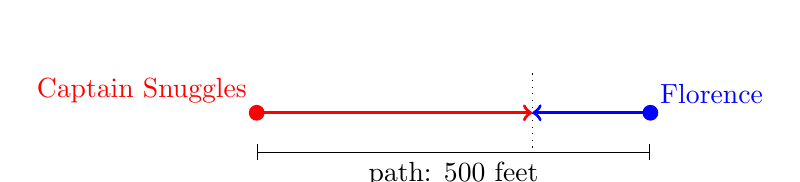
\begin{tikzpicture}
	\draw[|-|] (0,0) -- node[below]{path: 500 feet} (5,0);
	\draw[dotted] (3.5,1) -- (3.5,0);
	% gorilla
	\draw[red, very thick, ->] (0,0.5) -- (3.5,0.5);
	\fill[red] (0,0.5) circle[radius=0.1cm] node[above left]{Captain Snuggles};
	% zookeeper
	\draw[blue, very thick, ->] (5,0.5) -- (3.5,0.5);
	\fill[blue] (5,0.5) circle[radius=0.1cm] node[above right]{Florence};
\end{tikzpicture}
\end{center}%{figure}

The problem asks a question about time, so let's use $t$ to represent the time (in seconds) it takes for the two travelers to meet.

What else do we know from the problem? We have the speeds that both of the characters are moving.\footnote{We are also given the weight of the gorilla, although this is just a distraction and not important to the problem.} Florence moves at a speed of 4 feet per second, so in $t$ seconds she can travel $4t$ feet. Captain Snuggles can travel $26t$ feet in $t$ seconds. So, we can update our picture:
\begin{center}%{figure}
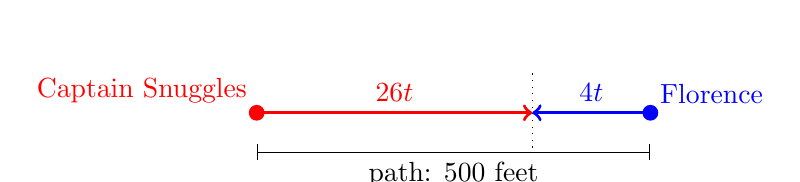
\begin{tikzpicture}
	\draw[|-|] (0,0) -- node[below]{path: 500 feet} (5,0);
	\draw[dotted] (3.5,1) -- (3.5,0);
	% gorilla
	\draw[red, very thick, ->] (0,0.5) -- node[above]{$26t$} (3.5,0.5);
	\fill[red] (0,0.5) circle[radius=0.1cm] node[above left]{Captain Snuggles};
	% zookeeper
	\draw[blue, very thick, ->] (5,0.5) -- node[above]{$4t$} (3.5,0.5);
	\fill[blue] (5,0.5) circle[radius=0.1cm] node[above right]{Florence};
\end{tikzpicture}
\end{center}%{figure}

From the drawing we can see that the combined distance that the two characters travel must be exactly 500 feet! So, we have our equation:
\[26t + 4t = 500\]
Again, we've got just a single linear equation and not a system. Who would have thought that such a complicated-looking problem would have a relatively simple mathematical representation!

%The problem is asks when Yeardleigh will pass Bob. In order to know when she will pass, we need to know when they have gone exactly the same amount of distance from the factory (this is the moment she passes him). So we'll write two distance equations, one for Bob and one for Yeardleigh, and compare them to try and figure out at what time their distances from the factories are equal.
%
%Our table columns are -- naturally enough -- rate, time, and distance. The rows deal with the people driving. The problem asks a ``when'' question, so we must be solving for time. Let's use $t$ to represent the amount of time Bob has been driving, in hours.
%
%Note that we didn't make the variable represent actual time ``on the clock''. (Why not? What challenges would that introduce into the mathematics?)
%


%%%%%%%%%%%%%%%%%%%%%%%%%%%%%%%%%%%%%%%%%%%%%%%%%%

\subsubsection{A trickier RTD problem}

\begin{boxex}
Florence the zookeeper, sadly, found herself on the business end of a hungry gorilla. Luckily, this occurred just outside the security hut, where the zoo's security squad witnessed the terrifying (but non-fatal) mauling. When they sounded the alarm, Captain Snuggles fled toward the zoo's entrance. The security squad gave chase along the same route 30 seconds later, after arming their tranquilizer guns and mounting their bicycles.

Captain Snuggles ran at 18 miles per hour. The security team cycled at 25 miles per hour, which was just fast enough: they reached the zoo entrance at the same moment as the gorilla and tranquilized him into submission. How much time elapsed between the sounding of the alarm and the tranquilizing of the gorilla? How far was the security hut from the zoo entrance?
\end{boxex}

Since the security squad started 30 seconds later, they have 30 seconds less travel time than Captain Snuggles. If we let $t$ represent the amount of time that Captain Snuggles is running (in seconds), then the security squad is chasing for $t-30$ seconds.

Even though Captain Snuggles has a head start, the security squad reaches the entrance at the same time as the gorilla because of their greater speed. So, both parties travel the same distance $d$.

Now, we have to be careful about units! The speeds in this problem are given in \emph{miles per hour}, and the time difference is given in \emph{seconds}. So, we could be careful to keep our units aligned. Let's use a little dimensional analysis (from \cref{ch:proportions}) to convert the speeds to ``feet per second''.\footnote{Alternatively, we could let $t$ represent time in minutes, and then convert the given speeds to distance \textit{per minute}. In that case, the security team would be in pursuit for $t=\frac{1}{2}$ minutes, since 30 seconds is half of one minute.}
\[
\begin{array}{r >{\displaystyle}l}
\text{Captain Snuggles:\quad}
&
\frac{18 \text{ miles}}{\text{hour}}
\cdot
\frac{5280 \text{ feet}}{\text{mile}}
\cdot
\frac{1 \text{ hour}}{3600 \text{ seconds}}
=
\frac{26.4 \text{ feet}}{\text{second}}
\\[\fracspace]
\text{Security Squad:\quad}
&
\frac{25 \text{ miles}}{\text{hour}}
\cdot
\frac{5280 \text{ feet}}{\text{mile}}
\cdot
\frac{1 \text{ hour}}{3600 \text{ seconds}}
=
\frac{36.\overline{6} \text{ feet}}{\text{second}}
\end{array}
\]

If we let $d$ represent the distance (in feet) from the security hut to the zoo entrance, then we can write an equation to describe the motion of Captain Snuggles:
\[d = 26.4t.\]
We can also model the motion of the security squad. Our formula shows both the different speed, and the fact that they start 30 seconds late:
\[d=36.\overline{6}(t-30).\]
These two equations comprise our system. Since we know that the security team and the gorilla arrive at the zoo at the same moment, we know that they travel the same amount of distance. In other words, $d$ is the same for both travelers. Substitution looks like a good choice for solving this system! (Can you explain why?)

%
%\begin{center}
%\begin{tabular}{r|ccc}
%				& Rate (mph)			& Time (hours)		& Distance (miles)\\\hline
%Bob				& 25					& $t$				& $25t$\\
%Yeardleigh		& 40					& $t - \frac{1}{2}$	& $40\left(t - \frac{1}{2}\right)$\\
%\end{tabular}
%\end{center}
%
%\[
%\left\{%
%\begin{aligned}
%&d = 25t\\
%&d = 40\left(t-\frac{1}{2}\right)
%\end{aligned}
%\right.
%\]
%
%Solving this system (substitution looks like a good choice!) will give us a value for $t$. What does that value represent? How can we use it to determine when (on the clock) Yeardleigh will pas Bob?


% % % % % % % % % % % % % % % % % % % % % % % % % % % % % % % % % % % % % % % %
\subsection{Motion in a current}

%Don't let that complicated-sounding name fool you, problems of this type are not that complicated to solve.

Have you ever tried to walk \textit{up} the \textit{down} escalator at the mall? (Be honest!) When you walk down the down elevator -- that is, when you walk in the same direction that the escalator is moving -- the motion of the escalator helps you to go faster than if you were just walking down regular stairs. On the other hand, if you try walk in the wrong direction on an escalator, the motion of the escalator will make you go slower than you would walk on regular stairs.

This is the idea of motion in a current. When you go ``with the current'' (or ``downstream'', if you're floating on a river) the current adds to your usual rate of motion. Going ``against the current'' (or ``upstream''), the current reduces your usual rate of motion.

%Bob decides to go on vacation. He takes a day trip on a river boat. The boat travels 60 km upstream (against the current) in 5 hours. The boat travels the same distance downstream in 3 hours. What is the rate of the boat in still water? What is the rate of the river's current?

\begin{boxex}
Bob and Yeardleigh were at the Cheeseville Zoo on a school field trip at the time of the mauling. When the alarm sounded, they both ran towards the escalators leading up the side of Mount Ploom toward the aviary. Yeardleigh, of course, ran up the up escalator. Bob, in a panic (and, well, because he's Bob), ran up the down escalator.

Yeardleigh reached the top in 19 seconds and Bob reached the top 23 seconds later. If the escalators are each 213 feet long, how fast were the twins running? How fast were the escalators moving? (Assume that the twins run at the same speed, and the two escalators move at the same speed.)
\end{boxex}

In this problem, we don't know either of the speeds. So, let's use $r$ to represent the running speed of the twins and $e$ to represent the moving speed of the escalators.

When Yeardleigh runs with the help of the escalator, she attains a speed of $r+e$. Bob, on the other hand, has his overall speed reduced by the movment of the escalator and moves at a speed of $r-e$.

\begin{center}
\begin{tabular}{r|ccc}
	& Rate (ft/sec)			& Time (sec)		& Distance (ft)\\\hline
Yeardleigh	& $r+e$		& 19			& 213\\
Bob			& $r-e$			& 42			& 213\\
\end{tabular}
\end{center}
Be sure to read carefully! Notice that the problem says Bob reaches the top 23 seconds \emph{later} than Yeardleigh. That means the trip takes him $19+23=42$ seconds. 

%Notice that Bob makes a round trip journey. So, the distance upstream is the same as the distance downstream. We don't know the speed of the water or the speed of the boat. So, let's let $b$ represent the speed of the boat, and $c$ represent the speed of the current.
%
%The boat goes $b-c$ km/hour upstream, because the current is taking away from how fast the boat can go. The boat will go $b+c$ km/hour downstream, because the current will help the boat go faster!
%
%\begin{center}
%\begin{tabular}{r|ccc}
%				& Rate (km/h)			& Time (hours)		& Distance (km)\\\hline
%Upstream		& $b-c$				& 5					& 60\\
%Downstream	& $b+c$				& 3					& 60\\
%\end{tabular}
%\end{center}
%
Given this setup, our system is:
\[
\left\{%
\begin{aligned}
&19(r+e) = 213\\
&42(r-e) = 213
\end{aligned}
\right.
\]
To solve this, we'll need the distributive property and the elimination method!


% % % % % % % % % % % % % % % % % % % % % % % % % % % % % % % % % % % % % % % % 
\chaptersummary

We learned a number of techniques in this section for writing and solving systems of linear equations -- graphing, substitution, and elimination -- and we now have all three approaches in our algebraic toolbox. Each of the techniques has its advantages and disadvantages, but together they make a powerful collection.

In the next chapter we will broaden our algebraic vocabulary, so to speak, by dropping the requirement that we always talk about \textit{equations}, or systems of \textit{equations}. Equality is important (in mathematics and in life), but we all know that things are not always in perfect balance. Onward!

\bigskip
\begin{boxcheese}
Florence the zookeeper made a full recovery, and Captain Snuggles successfully completed an anger management course and was reintroduced to the Cheeseville Zoo community. Unfortunately, the day's events were a public relations nightmare for the zoo. Annual attendance declined exponentially until 2003, at which point the zoo was purchased by YeardleighCorp.
\addtodoitem{Adjust year of YCorp takeover of Cheeseville Zoo.}
\end{boxcheese}

\chaptercopyright

\include{ch09_inequalities}
\include{ch10_expofunc}
\include{ch11_expoexpr}
\chapter{Quadratic equations}
\label{ch:quadeq}

\chapquote{We must say that there are as many squares as there are numbers.}{Galileo Galilei, Italian physicist and astronomer}

We saw quadratic patterns for the first time back in \cref{ch:sequences}, when we learned about quadratic sequences. We worked a bit with equations for quadratic data, but we haven't seen quadratic equations since then.\footnote{By the way, now might be a good time to have a second look at the final sections of \cref{ch:sequences}. Those are (;,;) sections, and so they may have been a bit challenging the first time around. You have a lot more algebra skills at this point in the course, though, and those sections might not be as daunting now!}

In \cref{ch:equations} we learned a set of tools in for solving linear equations. Many of those tools will be helpful here, but in this chapter, we'll also see what makes quadratic equations different from those we've studied until now. Our main task will be to develop techniques that will help us to overcome the trickier aspects of quadratic equations.

% % % % % % % % % % % % % % % % % % % % % % % % % % % % % % % % % % % % % % % % 
\section{Challenges to solving quadratics}

\begin{boxexplore}[A problem with quadratics]
Consider the following equation. Do we know what we need to know to solve this equation, without any guesswork? In other words: Do we have POEs, axioms, or other properties that will allow us to isolate $x$?
\[x^2 + 2x - 15 = 20\]
If you can, solve the equation. Otherwise, identify where you get stuck. What new tools would be helpful for solving this equation?
\end{boxexplore}

Our task in this chapter is to be able to solve quadratic equations like the one given in the startup exploration. We won't give the details for how to solve this equation yet -- we'll develop those ideas over the next few sections. For now, we will simply point out a few features.

Using what we know so far, it's impossible to isolate $x$. We can make some progress:
\[\begin{aligned}
x^2 + 2x - 15 &= 20
\\
x^2 + 2x &= 35
&&\quad\text{APOE, to get all the numbers to the right-hand side}
\end{aligned}\]
But now what? We can't combine like terms on the left-hand side, and subtracting anything from that side would give us $x$'s on both sides of the equation (making things worse). We might try undoing the distributive property on the left-hand side. That would give us
\[x(x+2)=35.\]
But this doesn't seem to be much of an improvement either. Using DPOE on the left-hand side to isolate $x$ would move $(x+2)$ to the right hand side of the equation (and vice versa). It seems that we'll need some other techniques to help us out of this situation.

If we're allowed to just solve the equation my making a clever observation, we might notice that \[5(7) = 5(5+2)=35,\] and so $x=5$ is a solution to the equation! That's progress. But, it might not be obvious that $-7$ is \textit{also} a solution to the equation, since \[-7(-7+2) = -7(-5) = 35.\] Plus with a different equation, it might not be quite so easy to see a solution just by inspection. What to do with $x(x+2)=29$, for example? Our new techniques should help us overcome these challenges.

\subsection{Rectangles and squares}

As we saw in \cref{ch:sequences}, quadratic sequences can be related to rectangles and squares. Our very first quadratic sequence was related to rectangles (\cref{fig:rects}), and so are the familiar perfect squares (\cref{fig:squares}).

\begin{figure}[!htbp]
\centering
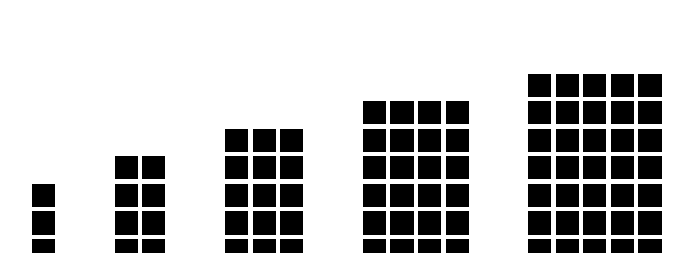
\begin{tikzpicture}[scale=0.35]
	\foreach \x in {0}
	\foreach \y in {0,...,2}
	\draw [ultra thick, white, fill=black] (\x,\y) rectangle (\x+1,\y+1);

	\begin{scope}[xshift=3cm]
	\foreach \x in {0,...,1}
	\foreach \y in {0,...,3}
	\draw [ultra thick, white, fill=black] (\x,\y) rectangle (\x+1,\y+1);
	\end{scope}

	\begin{scope}[xshift=7cm]
	\foreach \x in {0,...,2}
	\foreach \y in {0,...,4}
	\draw [ultra thick, white, fill=black] (\x,\y) rectangle (\x+1,\y+1);
	\end{scope}

	\begin{scope}[xshift=12cm]
	\foreach \x in {0,...,3}
	\foreach \y in {0,...,5}
	\draw [ultra thick, white, fill=black] (\x,\y) rectangle (\x+1,\y+1);
	\end{scope}

	\begin{scope}[xshift=18cm]
	\foreach \x in {0,...,4}
	\foreach \y in {0,...,6}
	\draw [ultra thick, white, fill=black] (\x,\y) rectangle (\x+1,\y+1);
	\end{scope}
\end{tikzpicture}
\caption{Some ``rectangular numbers'': $3, 8, 15, 24, 35, \dotsc$}
\label{fig:rects}
\end{figure}

\begin{figure}[!htbp]
\centering
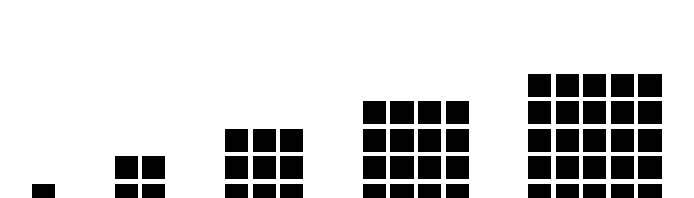
\begin{tikzpicture}[scale=0.35]
	\draw [ultra thick, white, fill=black] (0,0) rectangle (1,1);

	\begin{scope}[xshift=3cm]
	\foreach \x in {0,...,1}
	\foreach \y in {0,...,1}
	\draw [ultra thick, white, fill=black] (\x,\y) rectangle (\x+1,\y+1);
	\end{scope}

	\begin{scope}[xshift=7cm]
	\foreach \x in {0,...,2}
	\foreach \y in {0,...,2}
	\draw [ultra thick, white, fill=black] (\x,\y) rectangle (\x+1,\y+1);
	\end{scope}

	\begin{scope}[xshift=12cm]
	\foreach \x in {0,...,3}
	\foreach \y in {0,...,3}
	\draw [ultra thick, white, fill=black] (\x,\y) rectangle (\x+1,\y+1);
	\end{scope}

	\begin{scope}[xshift=18cm]
	\foreach \x in {0,...,4}
	\foreach \y in {0,...,4}
	\draw [ultra thick, white, fill=black] (\x,\y) rectangle (\x+1,\y+1);
	\end{scope}
\end{tikzpicture}
\caption{The perfect squares: $1, 4, 9, 16, 25, \dotsc$}
\label{fig:squares}
\end{figure}

The perfect squares have a straightforward formula. If we let $f(x)$ represent the area of figure $x$, then the perfect squares are represented by the formula
\[f(x)=x^2.\]
This is the parent function of the quadratic family.

The rectangles in \cref{fig:rects} also have a formula. If we let $g(x)$ represent the area of figure $x$, then we might notice that figure $x$ is $x$ units wide and $(x+2)$ units tall. So these rectangles are represented by the formula
\[g(x) = x(x+2).\]
We can simplify this formula using the distributive property:
\[g(x) = x(x+2) = x^2 + 2x\]

We have learned that the highest degree term in a quadratic equation is an $x^2$ term. The connection between a quadratic rule and rectangles will help us when it comes to solving quadratic equations. In fact, we will solve these equations using the beautiful symmetry of the square.

% % % % % % % % % % % % % % % % % % % % % % % % % % % % % % % % % % % % % % % % 
\section{Level 1 and 2 quadratics}

As we did with linear equations, we'll treat quadratic equations like a game. Level 1 is the easiest kind of quadratic equation to solve, so this is where we'll start. Then, we'll keep things interesting as we increase our skill level by adding challenge and complexity along the way.

\subsection{Level 1 quadratics}

\begin{boxexplore}[Quadratic level 1]
Determine the value of $x$ given the equation: $x^2 = 64$.
\end{boxexplore} %% End of startup exploration

Talk about starting with the easy stuff. We're looking for a number $x$ which, when multiplied by itself, is equal to 64. In other words, we are looking for the ``square root of 64''. Clearly, $x=8$ is a solution to this equation. But we can't be too hasty! Notice that $x=\umin8$ is also a solution, since $(\umin8)^2 = (\umin8)(\umin8) = 64$. So, this equation has two solutions:
\[x = 8 \OR \umin8\]
If we prefer to write our answer in solution set notation, we have \[\solset{8,\umin8}.\]

So, Level 1 quadratics are pretty easy: we simply take the square root of both sides of the equation.\footnote{More soon on square roots, including why and under what circumstances ``square root of both sides'' is, in fact, a property of equality.} We might have a hard time if the constant value is not a perfect square, as in $x^2 = 12$. But, we'll learn more about handling the square roots of non-perfect-squares soon enough (in \cref{ch:radicals}, to be precise).

This seems like a good time to suggest that it may come in handy to memorize the first 25 or so perfect squares, for quick recognition when they come up in a problem.
\begin{align*}
1^2 &= 1		&
2^2 &= 4		&
3^2 &= 9		&
4^2 &= 16		&
5^2 &= 25		\\
6^2 &= 36		&
7^2 &= 49		&
8^2 &= 64		&
9^2 &= 81		&
10^2 &= 100	\\
11^2 &= 121	&
12^2 &= 144 	&
13^2 &= 169 	&
14^2 &= 196 	&
15^2 &= 225 	\\
16^2 &= 256 	&
17^2 &= 289 	&
18^2 &= 324 	&
19^2 &= 361 	&
20^2 &= 400 	\\
21^2 &= 441 	&
22^2 &= 484 	&
23^2 &= 529 	&
24^2 &= 576 	&
25^2 &= 625 	\\
\end{align*}

Finally, note that zero is also a perfect square, since $0^2 = 0$. Zero, in fact, is the only number that has only one square root. Whereas both 3 and $\umin3$ are square roots of 9, the only square root of 0 is 0.

Finally, consider the square root of a negative number, say, $\umin25$. This is a bit of a problem. We're meant to find the the number that when multiplied by itself gives $\umin25$ as the result, but that's not going to work. Since we have a negative product, the two factors must have opposite signs! The best we can do is $5\cdot\umin5 = \umin25$ or $\umin5\cdot5 = \umin25$, and in these cases we're not multiplying a number times itself: 5 and $\umin5$ are different numbers!

So, there is no real number equal to the square root of $\umin25$. Of course, $\umin25$ isn't special, the same argument applies to any negative number. The moral of the story is this: If, as we go about solving a quadratic equation, we come to the point where we need to take the square root of a negative number, we have to stop and say that the equation has ``no real number'' as its solution. $\mathcal{S}=\emptyset$.


\subsection{Level 2 quadratics}

\begin{boxexplore}[Quadratic level 2]
Determine the value of $w$ given the equation: $(w+3)^2 = 16$.
\end{boxexplore} %% End of startup exploration

Here, we're told that something-squared is 16. Well, that means that the something in question must either be 4 or negative 4. That is to say, $(w+3)$ is either 4 or $\umin4$. So, this equation is actually two equations at once. We have:
\[w+3 = 4 \qquad\text{\underline{or}}\qquad w+3 = -4\]
Solving these equations (using SPOE in both cases), we have that $w$ must be either $1$ or $\umin7$. So, those are our two solutions: $\solset{1,\umin7}$.

We can record this work in a down-the-page format, like so:
\begin{align*}
(w+3)^2 &= 16
\\
w+3 &= 4 \OR \umin4
&&\text{square root of both sides}
\\
w &= 1 \OR \umin7
&&\text{SPOE: subtract 3 throughout}
\end{align*}

A few things to note: First, we can't subtract 3 from both sides as the very first step. The parentheses require that we undo the exponent first. Second, beware the use of $\pm$. It may be tempting to use this shorthand notation and write
\begin{align*}
w+3 &= \pm4,\\
\intertext{but then it is also tempting to subtract 3 and write}
w &= \pm1. \quad\text{Nope!}
\end{align*}
We recommend splitting into two equations, or writing out the two solutions explicitly using the word ``or''.

\begin{boxex}
Determine the value of $a$ given the equation: $(a-1)^2 - 2 = 23$.

\exsoln\ This equation requires an extra step, but it's quickly transformed into an equation like the one from the startup exploration.
\begin{align*}
(a-1)^2 - 2 &= 23
\\
(a-1)^2 &= 25
&&\text{APOE}
\\
a-1 &= 5 \OR \umin5
&&\text{square root of both sides}
\\
w &= 6 \OR \umin4
&&\text{APOE: add 1 throughout}
\end{align*}
In the end, we have $\solset{6, \umin4}$.
\end{boxex}

% % % % % % % % % % % % % % % % % % % % % % % % % % % % % % % % % % % % % % % % 
\section{Level 3 quadratics: Quadrangle method}

\begin{boxexplore}[Quadratic level 3]
Use the sum to a power property (from \cref{sec:exposumstopowers}) to write the expression $(x+3)^2$ without parentheses. Then, determine the value of $x$ given the equation: $x^2+6x+9 = 49$.
\end{boxexplore} %% End of startup exploration

To expand $(x+3)^2$, we might think of using algebra tiles to fill in a square with side length $(x+3)$. We used algebra tiles to solve this kind of problem back in \cref{sec:exposumstopowers}. Or, we could just ``sketch'' the algebra tiles diagram (shown below, on the right) and calculate the areas of the four regions.

\begin{minipage}{0.49\linewidth}
\centering
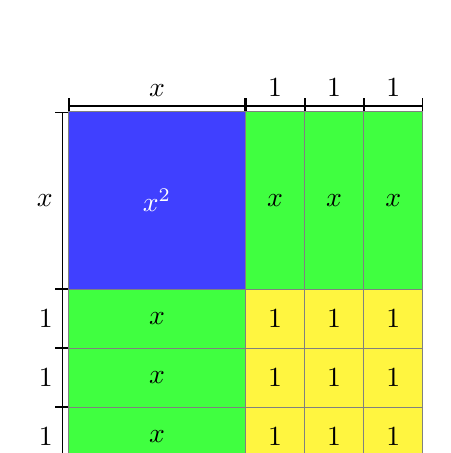
\begin{tikzpicture}[scale=0.75]
	\draw[|-|] (0,0.1) -- node[above]{$x$} (3,0.1);
	\draw[|-|] (-0.1,0) -- node[left]{$x$} (-0.1,-3);
	\draw[gray, fill=blue!75] (0,0) rectangle node[white]{$x^2$} (3,-3);
	\foreach \x in {3,...,5} {
		\draw[|-|] (\x,0.1) -- node[above]{1} (\x+1,0.1);
		\draw[gray, fill=green!75] (\x,0) rectangle node[black]{$x$} (\x+1,-3);
	}
	\foreach \y in {-3,...,-5} {
		\draw[|-|] (-0.1,\y) -- node[left]{1} (-0.1,\y-1);
		\draw[gray, fill=green!75] (0,\y) rectangle node[black]{$x$} (3,\y-1);
	}
	\foreach \x in {3,...,5} {
		\foreach \y in {-3,...,-5}
			\draw[gray, fill=yellow!75] (\x, \y) rectangle node[black]{1} (\x+1,\y-1);
	}
\end{tikzpicture}
\end{minipage}
%%
\begin{minipage}{0.49\textwidth}
	\quadrangle{x}{3}{x^2}{3x}{9}
\end{minipage}

Note how we have simplified the picture in the ``sketch'' version. For example, rather than draw three 3-unit-by-$x$-unit rectangles, we simply write the area of the rectangle $3x$. In the lower right-hand region, we write the area 9 rather than draw nine yellow squares.

We'll call this simplified sketch a \textit{quadrangle diagram}, and we'll call the method we are developing here the \textit{quadrangle method}.\footnote{The term \textit{quadrangle} is a synonym for \textit{rectangle}. History suggests that the term \textit{quadratic} is related to the term \textit{quadrangle} since this method of using square diagrams is so helpful in solving quadratic equations.} The quadrangle diagram can help us to see the relationship between the two expressions in the startup exploration:
\[(x+3)^2 = x^2 + 6x + 9.\]
Using this fact, we can solve the given equation:
\begin{align*}
x^2 + 6x + 9 &= 49
\\
(x+3)^2 &= 49
&&\text{based on the quadrangle diagram}
\\
x+3 &= 7 \OR \umin7
&&\text{square root of both sides}
\\
x &= 4 \OR \umin10
&&\text{SPOE: subtract 3 throughout}
\end{align*}
Can you see the clever trick that we used here? We rewrote an expanded expression as a something-squared expression, and then we solved it like a Level 2 quadratic!

Let's work through another example in detail, for example, solving the Level 3 equation
\[x^2 + 12x + 36 = 144.\]

Our goal is to write the left-hand side in a something-squared form. To do that, we'll begin by drawing an empty quadrangle diagram and filling in the bits that we know. For example, we know that the upper left-hand box must contain $x^2$, and so the sides of that square must each be $x$ units long.

\quadrangle{x}{}{x^2}{}{}

We know that the 36 will appear in the lower right-hand box. But how sould we label the side lenghts here? There are lots of combinations of numbers that multiply together to get 36\ldots

\quadrangle{x}{?}{x^2}{}{36}

Remember that the goal is to get an expression of the form something-\textit{squared}, and so we should always strive to create a quadrangle that is, in fact, a square. This means that we must choose 6 and 6 as the side lengths. If we chose another pair of factors, like 2 and 18, we would get the proper product in the lower right-hand region, but our overall diagram would no longer be a square.

\quadrangle{x}{6}{x^2}{}{36}

To fill in the remaining regions, we multiply the dimensions of each. In both cases we get $6x$. This is good news! Together these make $12x$ (which is what we have in the original, expanded expression). Plus, the two regions contain the same value, and so the beautiful symmetry of the square is preserved.

\quadrangle{x}{6}{x^2}{6x}{36}

So, we have rewritten our expression as a something-squared expression:
\[x^2 + 12x + 36 = (x+6)^2.\]
We can use this to solve the equation that we were given:
\begin{align*}
x^2 + 12x + 36 &= 144
\\
(x+6)^2 &= 144
&&\text{based on the quadrangle diagram}
\\
x+6 &= 12 \OR \umin12
&&\text{square root of both sides}
\\
x &= 6 \OR \umin18
&&\text{SPOE}
\end{align*}

\begin{boxex}
Determine the value of $n$ given the equation: $n^2 - 16n + 64 = 1$.

\exsoln\ Let's build the quadrangle diagram. The upper left-hand corner contains $n^2$, as above. To maintain symmetry, we should split the $-16n$ exactly in half. Don't worry about the negative coefficient, we can work with that. We should be on guard though for sign-related issues.

\quadrangle{n}{}{n^2}{-8n}{}

This tells us that the remaining portion of the square's side length must be $-8$. Let's not worry too much about the fact that negative distances are impossible\ldots\ the idea still works. This implies that the remaining region contains 64 (note, that positive 64). This agrees with the equation we were given.

\quadrangle{n}{-8}{n^2}{-8n}{64}

Now, we can solve the equation:
\begin{align*}
n^2 -16n +64 &= 1
\\
(n-8)^2 &= 1
&&\text{based on the quadrangle diagram}
\\
n-8 &= 1 \OR \umin1
&&\text{square root of both sides}
\\
n &= 9 \OR 7
&&\text{SPOE}
\end{align*}
So, we have $\solset{7,9}$. We can check our work by substituting our proposed solutions back into the original equation. First, we'll test $n=7$:
\begin{align*}
n^2 -16n +64 &= 1
\\
(7)^2 - 16(7) + 64 &\overset{?}{=} 1
\\
49 - 112 + 64 &\overset{?}{=} 1
\\
1 &\overset{\checkmark}{=} 1
\end{align*}
First, we'll check $n=9$:
\begin{align*}
n^2 -16n +64 &= 1
\\
(9)^2 - 16(9) + 64 &\overset{?}{=} 1
\\
81 - 144 + 64 &\overset{?}{=} 1
\\
1 &\overset{\checkmark}{=} 1
\end{align*}
\end{boxex}

% % % % % % % % % % % % % % % % % % % % % % % % % % % % % % % % % % % % % % % % 
\section{Level 4 quadratics: Adjust the constant term}

\begin{boxexplore}[Quadratic level 4]
Determine the value of $x$ given the equation: $x^2 + 8x + 15 = 99$.
\end{boxexplore} %% End of startup exploration

Let's try to build the quadrangle diagram. The upper left-hand corner contains $x^2$, as before. To maintain symmetry, we should split the $8x$ exactly in half. This tells us that the large square must be $(x+4)$ units on a side.

\quadrangle{x}{4}{x^2}{4x}{}

The problem is that, according to our quadrangle diagram, the lower right-hand corner should be 16\ldots\ but the equation we are given tells us to put 15 in that space. Now what? Our equation does not represent a complete square!

\quadrangle{x}{4}{x^2}{4x}{\color{red}15}

POEs to the rescue! Why not add 1 to both sides of the given equation to complete the square? This will give us the number we want on the left-hand side and, since we add 1 to both sides, we have an equivalent equation. So, instead of solving the equation
\[x^2 + 8x + 15 = 99,\]
we will add one to both sides and solve the equation
\[x^2 + 8x + 16 = 100.\]
Now, we can draw the quadrangle diagram exactly as we wanted.

\quadrangle{x}{4}{x^2}{4x}{16}

And now that we have a proper quadrangle diagram, we can solve the equation! Here's the full process:
\begin{align*}
x^2 + 8x + 15 &= 99
\\
x^2 + 8x + 16 &= 100
&&\text{APOE: add 1 to both sides}
\\
(x+4)^2 &= 100
&&\text{based on the quadrangle diagram}
\\
x+4 &= 10 \OR \umin10
&&\text{square root of both sides}
\\
x &= 6 \OR \umin14
&&\text{SPOE}
\end{align*}

This is a clever application of the POEs. Rather than use the properties to eliminate terms from one side of the equation, we can use the properties to change one side into a particular, more-helpful form.\footnote{In fact, this is exactly what we've been doing all along: changing one side of an equation into a form that is more helpful. In this chapter we are expanding our notion of what it means for a change to be ``helpful''.}

\begin{boxex}
Determine the value of $x$ given the equation: $x^2-6x+11=27$.

\exsoln\ When we start the quadrangle diagram, we split the $-6x$ as usual. This means that the square has sides of length $(x-3)$. This, in turn, implies that the lower right-hand region should be 9. Our equation has 11 as its constant term: not what we want.

\quadrangle{x}{-3}{x^2}{-3x}{\color{red}9}

To fix, this we can subtract 2 to each side of our equation. This will give us a constant term of 9, which is what we need to make our quadrangle diagram work. So, we have:
\begin{align*}
x^2 - 6x + 11 &= 27
\\
x^2 - 6x + 9 &= 25
&&\text{SPOE: subtract 2 from both sides}
\\
(x-3)^2 &= 25
&&\text{based on the quadrangle diagram}
\\
x-3 &= 5 \OR \umin5
&&\text{square root of both sides}
\\
x &= 8 \OR \umin2
&&\text{SPOE}
\end{align*}
So, our solutions are $\solset{8, \umin2}$.
\end{boxex}

% % % % % % % % % % % % % % % % % % % % % % % % % % % % % % % % % % % % % % % % 
\section{Level 5 quadratics: Adjust the linear term}

The last few levels have had ``polite'' middle terms, which have split evenly into two pieces. What happens if we get a linear term with an odd coefficient?

\begin{boxexplore}[Quadratic level 5]
Determine the value of $x$ given the equation: $x^2 + 3x + 1 = 5$.
\end{boxexplore} %% End of startup exploration

If we jump right in and try the quadrangle method, we start to get into fraction territory. If we want to split the $3x$ term exactly in half, then each piece would be $\frac{3}{2}$. Then, the quadrangle method would predict $\frac{9}{4}$ in the lower-right corner.

\quadrangle{x}{\frac{3}{2}}{x^2}{\frac{3}{2}x}{\color{red}\frac{9}{4}}

The lower-right corner isn't what we have in our equation, so we could use APOE and add $\frac{5}{4}$ to adjust both sides\ldots\ Hmm. Not pretty. To be clear, the quadrangle method will not let us down: if we keep going with the fractions, we will arrive at the correct answer! But, perhaps there is an alternative approach that avoids the fractions.

Here's a clever idea: We could use MPOE and multiply through by 2. This would give us a linear term with an even coefficient! In other words:
\[x^2 + 3x + 1 = 5 \quad\xrightarrow{\quad\text{multiply through by 2}\quad}\quad 2x^2 + 6x + 2 = 10\]
This fixes our odd coefficient problem, since now we can break the $6x$ up into two sets of $3x$. But, what do we do with that $2x^2$? We can't use $x$ and $2x$ as the side lengths, for although that gives is the correct product, we would no longer have a square.

\quadrangle{\color{red}?}{3}{2x^2}{3x}{}

Now, here's a \textit{really} clever idea. Let's multiply through by 2 \textit{again}. In other words, we will multiply the original equation by 4:
\[x^2 + 3x + 1 = 5 \quad\xrightarrow{\quad\text{multiply through by 4}\quad}\quad 4x^2 + 12x + 4 = 20\]
We still have an even linear coefficient, and now we can write $4x^2$ as $2x$ times $2x$. Note that we have to take that factor of 2 into account when we're figuring out the other dimensions of the square. Study our new diagram closely and be sure you understand where each of the labels comes from.
\begin{center}
	\quadrangle{2x}{3}{4x^2}{6x}{9}
\end{center}

We now find ourselves in a Level 4 situation: our equation has 4 as the constant term, whereas the quadrangle diagram predicts 9 as the constant term. No problem! We can add 5 to both sides, and continute the process as we did with Level 4 quadratics. Here's a summary of the whole process:
\begin{align*}
x^2 + 3x + 1 &= 5
&&\text{original equation}
\\
4x^2 + 12x + 4 &= 20
&&\text{MPOE: multiply both sides by 4}
\\
4x^2 + 12x + 9 &= 25
&&\text{APOE: add 5 to both sides}
\\
(2x+3)^2 &= 25
&&\text{based on the quadrangle diagram}
\\
2x+3 &= 5 \OR \umin5
&&\text{square root of both sides}
\\
2x &= 2 \OR \umin8
&&\text{SPOE}
\\
x &= 1 \OR \umin4
&&\text{DPOE}
\end{align*}

Let's pause and review. When faced with an odd coefficient for the $x$ term, our strategy is to multiply through by 4. This will give us an even coefficient for the $x$ term, and at the same time keep the coefficient of the $x^2$ term in a state where it can be written as something times itself: $4x^2 = 2x\cdot2x$. After we do this, we'll have a Level 4 quadratic on our hands, and we can apply techniques for handling those.

\begin{boxex}
Determine the value of $x$ given the equation: $x^2-5x+12=62$.

\exsoln\ Faced with an odd linear coefficient, we multiply through by 4. This gives us the revised equation \[4x^2-20x+48=248.\] We set up the quadrangle diagram and see whether our equation represents a complete square.

\quadrangle{2x}{-5}{4x^2}{-10x}{\color{red}25}

Our (revised) equation does not make a proper square: the constant term in the equation is 48, but the quadrangle diagram predicts 25. We can fix this problem using SPOE: subtract 23 from both sides:
\begin{align*}
x^2 - 5x + 12 &= 62
&&\text{original equation}
\\
4x^2 - 20x + 48 &= 248
&&\text{MPOE: multiply both sides by 4}
\\
4x^2 - 20x + 25 &= 225
&&\text{SPOE: subtract 23 from to both sides}
\\
(2x-5)^2 &= 225
&&\text{based on the quadrangle diagram}
\\
2x-5 &= 15 \OR \umin15
&&\text{square root of both sides}
\\
2x &= 20 \OR \umin10
&&\text{SPOE}
\\
x &= 10 \OR \umin5
&&\text{DPOE}
\end{align*}
So in the end, we have solutions $\solset{10, \umin5}$.
\end{boxex}

% % % % % % % % % % % % % % % % % % % % % % % % % % % % % % % % % % % % % % % % 
\section{Level 6 quadratics: Adjust the quadratic term}

We've arrived at the highest level of the quadratic equation challenge! Until now, all of our equations have started with just $x^2$. What if the coefficient of the leading term is something other than 1?

\begin{boxexplore}[Quadratic level 6]
Determine the value of $x$ given the equation: $3x^2 + 8x + 1 = 12$.
\end{boxexplore} %% End of startup exploration

What shall we do in this scenario? A clever idea is to use DPOE and divide through by 3. That would make the leading coefficient 1, as in the earlier problems. The downside is that most of the other numbers turn into fractions.
\[3x^2 + 8x + 1 = 12
\quad\xrightarrow{\quad\text{divide through by 3}\quad}\quad
x^2 + \frac{8}{3}x + \frac{1}{3} = 4\]
The quadrangle method will absolutely work on an equation like this, but perhaps we'd prefer an approach that avoided all the fractions.

If scaling the equation down doesn't help, why not try to scale it up? Could we multiply through by some helpful value? Recall that the goal will be to write the $x^2$ term as something times itself. Since there's already a 3 there, we can solve our problem if we multiply through by 3.
\[3x^2 + 8x + 1 = 12
\quad\xrightarrow{\quad\text{multiply through by 3}\quad}\quad
9x^2 + 24x + 3 = 36\]
Note that now we are in a good position, since $9x^2 = 3x\cdot3x$. So, let's fill out our quadrangle diagram. We have an even coefficient on the linear term, so we can split that evenly. Note that we have to take all the coefficients into account when completing the diagram. For example, when figuring out the dimensions of a box containing $12x$.

\quadrangle{3x}{4}{9x^2}{12x}{\color{red}16}

The quadrangle diagram predicts 16 as the constant term, and so our equation is not a complete square. We can use APOE to fix that, adding 13 to both sides. Here's how it goes:
\begin{align*}
3x^2 +8x + 1 &= 12
&&\text{original equation}
\\
9x^2 + 24x + 3 &= 36
&&\text{MPOE: multiply through by 3}
\\
9x^2 +24x + 16 &= 49
&&\text{APOE: add 13 to both sides}
\\
(3x+4)^2 &= 49
&&\text{based on the quadrangle diagram}
\\
3x+4 &= 7 \OR \umin7
&&\text{square root of both sides}
\\
3x &= 3 \OR \umin11
&&\text{SPOE}
\\
x &= 1 \OR \umin\tfrac{11}{3}
&&\text{DPOE}
\end{align*}

In summary, we multiplied through by the coefficient of the $x^2$ term, which gave us a coefficient that was a perfect square. In the final example for this chapter, we put it all together.

\begin{boxex}
Determine the value of $x$ given the equation $-5x^2-x+18=0$.

\exsoln\ Since we have a leading coefficient that is not a perfect square, we multiply through by that coefficient, $-5$ in this case. This gives us
\[25x^2+5x-90=0\]
(careful with the negative signs). This is an improvement, but we have a linear coefficient that is odd. So, we multiply by 4 to fix that:
\[100x^2 + 20x - 360=0\]
Notice that multiplying through by 4 (a perfect square) gives us a leading coefficient that is still a perfect square. This is because the product of two perfect squares is itself a perfect square! (Can you prove that this statement is always true using the properties of exponents?)

We now have a revised equation that we can bring to the quadrangle method.

\quadrangle{10x}{1}{100x^2}{10x}{\color{red}1}

To get our constant terms to agree, we must add 361 to both sides of our revised equation. This gives us
\[10x^2 + 10x + 1 = 361.\]
And from here, we can complete a familiar process.
\begin{align*}
10x^2 +10x + 1 &= 316
&&\text{}
\\
(10x+1)^2 &= 316
&&\text{based on the quadrangle diagram}
\\
10x+1 &= 19 \OR \umin19
&&\text{square root of both sides}
\\
10x &= 18 \OR \umin20
&&\text{SPOE}
\\
x &= \tfrac{18}{10} \OR \umin2
&&\text{DPOE}
\end{align*}
After we simplify our one fraction answer, we have a final solution: $\solset{\frac{9}{5}, \umin2}$.
\end{boxex}

\subsection{(;,;) Quadratic formula}
\label{sec:quadformulapreview}

Now that we have the quadrangle method at our disposal, we can tackle any quadratic equation that is thrown at us. We might be tempted to really get generic, and solve the all at once.

Consider a completely generic quadratic equation of the form \[ax^2 + bx + c=0.\] This quadratic has three coefficients: $a$ is the coefficient of the quadratic term, $b$ is the coefficient of the linear term, and $c$ is the constant term. We've set it equal to zero for reasons that will be made clear in a few chapters.\footnote{Sorry for the mystery, but all will be revealed soon. In the meantime, note that we can always turn a quadratic equation into this form. If we have an equation that does not equal zero, for example $ax^2 + bx + c = d$ where $d$ is not zero, then we can use SPOE to get 0 on the right-hand side: $ax^2+bx+c-d=0$. Then, we pull a little algebraic sleight of hand, and replace $c-d$ with just $c$. This might look like an illegal move, but in the general form of a quadratic, ``$c$'' just stands for a constant value. Since ``c-d'' is a contstant value, we pretend that this was the constant value we meant all along.}

What happens if we apply the quadrangle method to this totally generic equation? We don't really know anything about $a$, so to be safe, let's multiply the whole equation by $a$. 
\[a^2x^2 + abx + ac=0.\]
This will ensure that the leading term is a perfect square, and that's what we need for the box method. Now, the linear coefficient is $ab$ and this might be an odd number for all we know. So, we multiply through by 4, as we have often done above.
\[4a^2x^2 + 4abx + 4c=0.\]
This is not a pretty sight, but we'll try to make it work with the quadrangle method.

\quadrangle{2ax}{b}{4a^2x^2}{2abx}{\color{red}b^2}

Much of this looks workable, but what about the lower right-hand corner? The quadrangle method predicts $b^2$, but our equation has $4c$. Well, we'll do what we usually do: we'll use the POEs to turn our left-hand side into the form we want. So:

\begin{align*}
4a^2x^2 + 4abx + 4c &= 0
&&\text{}
\\
4a^2x^2 + 4abx &= -4c
&&\text{SPOE: subtract $4c$ from both sides}
\\
4a^2x^2 + 4abx +b^2 &= b^2-4c
&&\text{APOE: add $b^2$ to both sides}
%
\intertext{It might seem like things are getting worse, but now the left-hand side is what we need to use our quadrangle diagram. Let's go!}
%
(2ax+b)^2 &= b^2-4c
&&\text{based on the quadrangle diagram}
\\
2ax+b &= \pm\sqrt{b^2-4c}
&&\text{square root of both sides}
\\
2ax &= \pm\sqrt{b^2-4c}-b
&&\text{SPOE: subtract $b$ from both sides}
\\[1ex]
x &= \frac{\pm\sqrt{b^2-4c}-b}{2a}
&&\text{DPOE: divide both sides by $2a$}
\\[1ex]
x &= \frac{-b\pm\sqrt{b^2-4c}}{2a}
&&\text{rearranging the numerator}
\end{align*}

That last rearrangement in the numerator is because it looks a little better, and to make it clear that the $-b$ isn't underneath the radical along with that other stuff. Also, it's tradition. This formula is a famous thing, and traditionally appears in this form.

% % % % % % % % % % % % % % % % % % % % % % % % % % % % % % % % % % % % % % % % 
\chaptersummary

The properties of equality which we learned before this chapter weren't enough to solve any random quadratic equation. To overcome the quadratic obstacle, we learned new techniques for solving quadratic equations. These new techniques are based on the symmetry of a square, and we learned various techniques for adjusting a quadratic equation so that we can use our new quadrangle method.

We have, however, avoided the necessity of finding the square root of a number that was not a perfect square. This was a helpful simplification -- it allowed us to focus on the process of equation solving -- but not all quadratics will have answers that come out so ``nice''. We turn our attention to square roots in the next chapter.

\chaptercopyright
\chapter{Radical expressions}
\label{ch:radicals}

\newcommand*\rfrac[2]{{}^{#1}\!/_{#2}}

\chapquote{There is geometry in the humming of the strings, there is music in the spacing of the spheres.}{Pythagoras, Ancient Greek philosopher}

In the last chapter, we found integer solutions to nearly all of the equations that we studied. This was good for understanding the workings of quadratic equations, but not all equations will necessarily be so ``polite''. The main focus of our work in this chapter is around understanding more about all of those square roots that don't come out evenly. We begin by looking more closely at the sets $\Q$ and $\R$.

% % % % % % % % % % % % % % % % % % % % % % % % % % % % % % % % % % % % % % % % 
\section{Real numbers}
\label{sec:radrealnumbers}

\begin{boxexplore}[Share the cheese]
Middle Market sells mini-wheels of cheese for snacking. Mini-wheels can be sold one at a time, or in boxes of 10. The cheese arrives at the warehouse in crates of 10 boxes (containing 100 wheels of cheese in total).

The warehouse workers need to divide their stock of mini-wheels up among three trucks, each of which will deliver to a local Middle Market branch. The warehouse has a total of 13 crates, 7 boxes, and 9 mini-wheels in stock.

The manager allows the workers to open crates or boxes, if needed, to divide the supply evenly. Describe a process for dividing up the cheese that requires opening the minimum number of boxes.
\end{boxexplore}

In \cref{ch:numbers}, we made some comments which might, at first, appear contradictory. On the one hand, we saw that the set of real numbers, $\R$, includes every possible decimal number. We also saw that the set of rational numbers, $\Q$, includes ``terminating decimals and repeating decimals''. 

On the other hand, we know that $\Q$ is the set of fractions, meaning those numbers that can be expressed in the form \[\frac{a}{b} \text{ where $a$ and $b$ are integers, and $b$ is not zero.}\]
These statements raise a few questions. What is the relationship between ``fraction'' and ``terminating or repeating decimal''? What can we say about decimal numbers that are neither terminating nor repeating?

\subsection{Fractions into decimals}

Recall that a fraction is simply a divison problem in disguise. If we execute the division problem, we can easily turn a fraction into a decimal. It's especially easy if we have a calculator handy\ldots\ otherwise, we're in for some long division.

\subsubsection{Long division}

Don't worry if your long division is a bit rusty, just take another look at the startup exploration. The warehouse workers must divide 1379 mini-wheels of cheese among the three trucks (that's $1379 \div 3$) but they must do this with a minimum amount of regrouping.

One solution is to put 4 crates on each of the three trucks. This takes care of 12 crates (1200 mini-wheels in all), but leaves one crate. They have no choice but to open this crate and treat it as 10 boxes. Of course they already had 7 boxes in stock, so now they have 17 boxes in all. They can put 5 boxes on each truck (accounting for 15 boxes, or 150 mini-wheels), but they will have 2 boxes left over. They open these two boxes, revealing 20 mini-wheels. They add these to the 9 mini-wheels they had already, giving 29 mini-wheels in all. Each truck gets 9 of these (using up 27), and they have 2 left over.

So, in the end: each truck gets 4 crates, 5 boxes, and 9 mini-wheels -- that's 459 mini-wheels in all -- and there are 2 left behind. Now have a look at the long division for this problem: can you spot each of the steps that we took above in the work below?

\[
\renewcommand\arraystretch{1.1}
\begin{array}{*1r @{\hskip\arraycolsep}c@{\hskip\arraycolsep} *4r}
	&&			& 4	& 5 & 9\\
\cline{2-6}
3	&\big)&	1	& 3	& 7 & 9\\
	&&		1	& 2	& 0	& 0\\
\cline{3-6}
	&&			& 1	& 7 & 9\\
	&&			& 1	& 5	& 0\\
\cline{4-6}
	&&			& 	& 2	& 9\\
	&&			&	& 2	& 7\\
\cline{5-6}
	&&			& 	& 	& 2\\
\end{array}
\]

In the cheese example, it makes sense to stop here with a remainder of 2. In general, though, we could continue the process of division and create a number that extends to the right of the decimal point.

\begin{boxex}
Convert $\dfrac{3}{4}$ and $\dfrac{1}{6}$ into their decimal representations.

\bigskip\inlineex{Solution:} Recall that the fraction three-fourths is equivalent to the division problem $3 \div 4$. To do this by long division, we put the dividend (that's 3) inside the ``division house'' and leave the divisor (that's 4) outside.
\[
\renewcommand\arraystretch{1.1}
\begin{array}{*1r @{\hskip\arraycolsep}c@{\hskip\arraycolsep} *3r}
	&&			0& .7	& 5 \\
\cline{2-5}
4	&\big)&	3	& .0	& 0 \\
	&&		2	&8		\\
\cline{3-4}
	&&			&2 & 0 \\
	&&			&2 & 0 \\
\cline{4-5}
	&&			&& 0 \\
\end{array}
\]
So the decimal representation of $\frac{3}{4} = 0.75$ (you may have known that already). To tackle one-sixth, we note that it is equivalent to $1 \div 6$. The long division starts out like this:
\[
\renewcommand\arraystretch{1.1}
\begin{array}{*1r @{\hskip\arraycolsep}c@{\hskip\arraycolsep} *4r}
	&&			0& .1	& 6	& 6 \\
\cline{2-6}
6	&\big)&	1	& .0	& 0	& 0 \\
	&&		0	&6		\\
\cline{3-4}
	&&			&4	& 0 \\
	&&			&3	& 6 \\
\cline{4-5}
	&&			&	& 4	& 0 \\
	&&			&	& 3	& 6 \\
\cline{5-6}
	&&			&	&	& 4
\end{array}
\]
We might as well stop here, though, because we're stuck in a loop! The 6's in the answer are going to repeat forever. (Can you see why?) So, the decimal representation of $\frac{1}{6} = 0.1\overline{6}$.
\end{boxex}

We say that $0.75$ is a terminating decimal, because the process of long division stops with a remainder of zero. On the other hand, $0.1\overline{6}$ is called a repeating decimal because the long division process gets stuck in a loop. Note that we've used a vinculum over the 6 to indicate which digits repeat.

When it comes to a division problem like $1 \div 6$ on a calculator, the display will likely show \texttt{0.166666667}, where the 6's repeat for a while and are followed by a 7. Don't be fooled by this 7: the 6's really do go on forever! That 7 is the calculator rounding up. Always be skeptical about the rightmost digit on your calculator screen.

\subsubsection{A bold claim}

This process of division leads us to make a pretty bold claim: every rational number can be represented \textit{either} as a terminating decimal or a repeating decimal. How can we be sure that every crazy fraction, for instance $\frac{19}{81}$, either terminates or repeats?

Let's think about how long division works: the ``subtraction step'' in particular. Here's how the process of long division starts out for $\frac{3}{4}$:
\[
\renewcommand\arraystretch{1.1}
\begin{array}{*1r @{\hskip\arraycolsep}c@{\hskip\arraycolsep} *3r}
	&&			& .7	&	\\
\cline{2-5}
4	&\big)&	3	& .0	& 0 \\
	&&		2	&8		\\
\cline{3-4}
	&&			&2 & 	\\
\end{array}
\]
In the subtraction step, we get 2 as the remainder, and so we know that we have to keep dividing. If we ever get the remainder 0, then we know that we're done with division. This is what happens eventually with $\frac{3}{4}$. On the other hand, if we ever get a remainder that we've gotten before, then we know that we're stuck in a loop. This is what happened with $\frac{1}{6}$.

Now here's a simple yet profound idea: the remainder is always less than the divisor. When dividing by 4, the remainder has to be less than 4. When dividing by 6, the remainder has to be less than 6. (Can you explain why that is? For example, when dividng mini-wheels of cheese among three trucks, could the workers have seven mini-wheels of cheese left over?)

The result is that we have a limited number of choices for the remainder. When dividing by 4, the remainder can only be 0, 1, 2, or 3. When dividing by 6, the remainder can only be : 0, 1, 2, 3, 4, or 5.

Having a limited number of choices means that eventually we have to recycle one of those remainders! We can't go on forever without either using the remainder 0 (in which case the decimal terminates) or reusing one of the nonzero remainders (in which case the decimal repeats).

Even when dividing something ugly like $1903 \div 8167$, the remainders in the subtraction steps will always be less than 8167. We might have to divide for a long time, but we know it can't carry on forever. Eventually we'll either use the remainder 0, or reuse a remainder we've used already. So the fraction $\frac{1903}{8167}$ has a decimal representation that either terminates or repeats.

Our argument applies to any denominator, and so to any rational number. Therefore, it's true that every rational number has a decimal representation that either terminates or repeats! Have we blown your mind yet? If not, stay tuned.

\subsection{Decimals into fractions}

What about the other way around? Does every terminating-or-repeating decimal have a corresponding fraction representation?

\subsubsection{Terminating decimals into fractions}

Consider a terminating decimal like $0.375$. Can we turn this decimal into a fraction, meaning a ratio of two integers? If so, how?

Recall the notion of \textit{place value}, and how the individual digits in a number are each standing in some ``place'' that is named after a power of ten.\footnote{We really are blowing the cobwebs off of some old mathematics in this chapter: Long division! Place value! It goes to show that even simple mathematical ideas can have deep and meaningful consequences.} The key to turning a terminating decimal into a fraction is recalling how to read a decimal using its place value.

\begin{center}
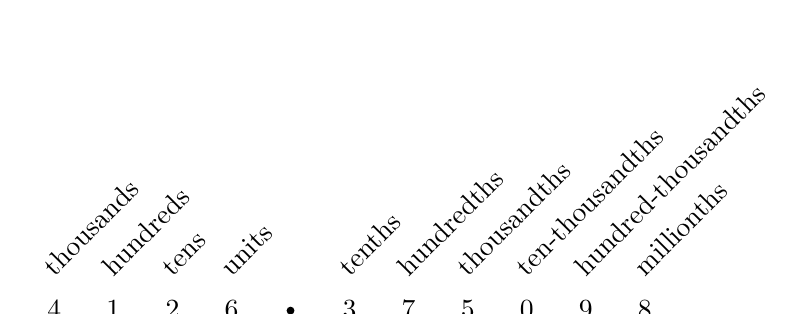
\begin{tikzpicture}
	\foreach \x in {0.75} {
		\draw (-4*\x,0) node[below]{4};
		\draw (-4*\x,0) node[above, anchor=south west, rotate=45]{thousands};
		\draw (-3*\x,0) node[below]{1};
		\draw (-3*\x,0) node[above, anchor=south west, rotate=45]{hundreds};
		\draw (-2*\x,0) node[below]{2};
		\draw (-2*\x,0) node[above, anchor=south west, rotate=45]{tens};
		\draw (-1*\x,0) node[below]{6};
		\draw (-1*\x,0) node[above, anchor=south west, rotate=45]{units};
		\fill (0,-0.25) circle[radius=0.05];
		\draw (1*\x,0) node[below]{3};
		\draw (1*\x,0) node[above, anchor=south west, rotate=45]{tenths};
		\draw (2*\x,0) node[below]{7};
		\draw (2*\x,0) node[above, anchor=south west, rotate=45]{hundredths};
		\draw (3*\x,0) node[below]{5};
		\draw (3*\x,0) node[above, anchor=south west, rotate=45]{thousandths};
		\draw (4*\x,0) node[below]{0};
		\draw (4*\x,0) node[above, anchor=south west, rotate=45]{ten-thousandths};
		\draw (5*\x,0) node[below]{9};
		\draw (5*\x,0) node[above, anchor=south west, rotate=45]{hundred-thousandths};
		\draw (6*\x,0) node[below]{8};
		\draw (6*\x,0) node[above, anchor=south west, rotate=45]{millionths};
	}
\end{tikzpicture}
\end{center}

To read the decimal 0.375, we can say ``zero point three seven five'', but this isn't very helpful. Instead, we read the number using place value and say ``three hundred seventy-five \textit{thousandths}''. Now, if someone were to say that number aloud, it sounds just like the fraction \[\frac{375}{1000}.\] In fact, this decimal number and this fraction represent exactly the same value. Of course, the fraction isn't in simplest form yet, but that's easy to fix: \[0.375 = \frac{375}{1000} = \frac{3}{8}\].

We have accomplished the goal of turning a terminating decimal into a fraction. The technique is simply to read the decimal aloud using its place value, and then write down the fraction we hear.

\subsubsection{Repeating decimals into fractions}

The ``read the number with its place value'' technique won't work for repeating decimals. (Why not?) Instead, we'll use some clever applications of the techniques we learned when solving equations.

Suppose we try to write the repeating decimal $0.\overline{4}$ as a fraction. Let's give this number a name so that we can do some algebraic manipulations. \[x = 0.\overline{4}\] Our goal will be to find an alternative way of writing $x$. To do that, we're going to make two clever moves.

The first clever move is to use MPOE: we will multiply both sides of this equation by 10. Multiplying $0.\overline{4}$ by 10 moves the decimal point one place to the right. But remember, the 4's repeat \textit{forever}, so there are \textit{still infinitely many} 4's to the right of the decimal point! We have: \[10x = 4.\overline{4}\]

The second clever move is to use an idea from when we were solving systems of equations: the elimination method. Watch what happens when we subtact the first equation we wrote from the second equation:

\[\begin{aligned}
	&&	10x &= 4.\overline{4}\\
- 	&& 	x 	&= 0.\overline{4}\\\hline
	&&	9x 	&= 4.0
\end{aligned}\]

Notice that the two numbers on the righthand side of our equations are exactly four units apart. In other words: the infinitely long tail of 4's disappears when we subtract! Now all we have to do is use DPOE to isolate $x$: \[9x = 4 \quad\implies\quad x = \frac{4}{9}\] If you have a calculator handy, you can perform this division and see that we have accomplished the goal of turning our repeating decimal into a fraction:\[0.\overline{4} = \frac{4}{9}\]

This process is sometimes called \textit{killing the tail}, since our goal is to subtract two different decimal forms that have the same repeating part, thereby eliminating the infintely long tail of digits.\footnote{An alternative technique, which we'll discuss in Algebra 2, involves turning the repeating decimal into an infinitely long sequence of ever-decreasing numbers, and then finding the sum of that sequence. Yes, we can -- in certain circumstances -- add up infinitely many numbers. This is just one of the amazing things that awaits you in Algebra 2!}

\begin{boxex}
Convert the repeating decimal $0.\overline{63}$ to its decimal representation.

\exsoln\ We'll kill the tail again, but note that we have two digits after the decimal which repeat. This will require a slight adjustment. We'll start as we did before, by assigning an algebraic name to our number:\[x = 0.6363\dotso\]
If we multiply both sides by 10, we'll have \[10x = 6.3636\dotso\] which is also a repeating decimal, but with a \textit{different} repeating tail. We could work with this, but it's a bit easier to multiply by 10 again (in other words, to multiply the original equation by 100): \[100x = 63.6363\dotso\] Now we have an equation in which the number on the righthand side has exactly the same tail as in the original equation. So, we subtract:
\[\begin{aligned}
	&&	100x	&= &63.\overline{63}\\
- 	&& 	x 		&= &0.\overline{63}\\\hline
	&&	99x 	&= &63.00
\end{aligned}\] We divide both sides by 99, and then simplify our fraction to lowest terms. In the end, we have: \[0.\overline{63} = \frac{63}{99} = \frac{7}{11}\]
\end{boxex}

The moral of the story is that we may have to adjust our method and choose the ``just right'' powers of 10. Consider how we might use kill the tail to turn $0.1\overline{6}$ back into $\frac{1}{6}$? (Note that the 6 repeats in the decimal form, but the 1 does not.)

Let's pause to reflect. In the first part of this section, we explained why every fraction can be written as either a terminating or repeating decimal. We can make this conversion using long division. Then we went on to show the reverse: that every terminating decimal can be written as a fraction (by reading it with its place value) and every repeating decimal can be written as a fraction (by killing the tail).

Armed with these tools, we might get the idea that \textit{every decimal} number can be turned into a fraction. Unfortunately (or fortunately, depending on how you look at it), this is not the case.

\subsection{Existence of irrational numbers}

The \glspl{irrational number} are all of the real numbers that are not rational numbers. In other words, those decimal numbers that cannot be expressed as either a terminating or repeating decimal.

Back in \cref{ch:numbers} we gave an example of such a number: \[0.10\,110\,1110\,11110\,111110\ldots\]
This number clearly has a pattern. We might explain it by saying: ``After the decimal point write one, then zero, the 2 ones, then zero, then 3 ones, then zero, and so on, always writing 1 more one than you did the last time.'' The problem is that is does not terminate (our pattern will continue forever), but it doesn't repeat either. The strings of 1's get longer and longer. There is never a set of always-repeating digits to group under a vinculum.

This single number is enough to prove that irrational numbers exist. Of course, there are lots of them. The famous number $\pi$ is irrational, and in some sense is even more diabolical.
\[\pi \approx 3. \, 1415926535 ~ 8979323846 ~ 2643383279 ~ 502884197 ~ 6939937510 ~ 5820974944 ~ 5923078164\ldots\]
This number doesn't even have a pattern that we can use to describe it (as far as we know). The digits go on infinitely, and come in a random sequence.

You may be wondering, ``How do we know $\pi$ is irrational?'' After all, it may be clear why the first number with the ones and zeros is irrational, but how to we know for sure that $\pi$ never terminates and never repeats?

Unfortunately, explaining the irrationality of $\pi$ requires a bit more mathematics that we can get into here. However, we have learned enough to prove that certain other numbers are irrational. More on that at the end of \cref{sec:radsquareroots}.

% % % % % % % % % % % % % % % % % % % % % % % % % % % % % % % % % % % % % % % % 
\section{Square roots}
\label{sec:radsquareroots}

We have already worked quite a bit with exponents, but every exponent so far has been an integer. Could we have a rational number as an exponent? If so, what would it mean?

\begin{boxexplore}[Half power]
Consider the expression \[9^{1/2},\] that is, ``nine to the power one-half''. What are some possible interpretations of this?

Use a calculator to explore what happens when we raise certain numbers to the one-half power (start with the natural numbers between 1 and 20). What patterns do you notice? What conjectures do you have about what's happening?
\end{boxexplore}

Suppose we let $x = 9^{1/2}$. We'd like to find an alternative way of expressing $x$ that uses only integer exponents. One approach is to multiply each side of this equation by itself. Then we'd have:
\[\begin{aligned}
x 			&= 9^{1/2}\\
x\cdot x 	&= 9^{1/2} \cdot 9^{1/2}
&&\quad\text{multiply each side by itself}\\
x\cdot x	&= 9^{(1/2)\,+\,(1/2)}
&&\quad\text{product rule for exponents}\\
x\cdot x	&= 9^{1}\\
x\cdot x	&= 9
\end{aligned}\]
So, $x$ is the number that when multiplied by itself gives $9$ as the result. That could be either $3$ or $\umin3$, since $3\cdot 3 = \umin3 \cdot \umin3 = 9$. Using some vocabulary that we already know: we say that $9^{1/2}$ is a \textit{square root} of $9$.

\begin{boxdef}[Square root]
A \gls{square root} of $a$ is a number $b$ such that $b \cdot b = a$.
\end{boxdef}

The reason this is called a ``square root'' has to do with the geometric interpretation of this operation. If we have a square of side length $\mathcal{S}$, then the area of the square is $\mathcal{S}^2$. Conversely, if we have a square with area $\mathcal{A}$, then the \textit{square root of $\mathcal{A}$} gives us the side length of the square. 

\begin{center}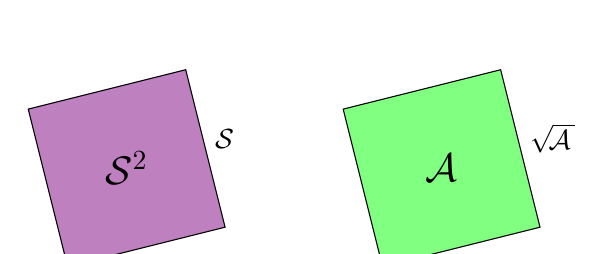
\begin{tikzpicture}[scale=0.5]
	\draw[fill=violet!50] (0,0) -- (4,1) -- (3,5) -- (-1,4) -- cycle;
	\draw (3.5,3.25) node[right]{$\mathcal{S}$};
	\draw (1.5, 2.5) node{\Large$\mathcal{S}^2$};
	\draw[fill=green!50] (8,0) -- (12,1) -- (11,5) -- (7,4) -- cycle;
	\draw (11.5,3.25) node[right]{$\sqrt{\!\mathcal{A}\,}$};
	\draw (9.5, 2.5) node{\Large$\mathcal{A}$};
\end{tikzpicture}\end{center}

Positive numbers have two square roots: one positive, one negative. Both 3 and $\umin3$ are square roots of 9, since $(3)(3) = 9$ and $(\umin3)(\umin3) = 9$. Zero is the only number that has exactly one square root: the square root of 0 is 0. Negative numbers cause some problems when it comes to square roots (stay tuned for more on that).

Most of the time, we'll be working with the positive square root of a number, called the \gls{principal square root} For example, the principal square root of 9 is 3 and the principal square root of 25 is 5.

The checkmark-ish symbol we use to denote the square root of $a$ is called the \gls{radical}: $\sqrt{a}$. This symbol means ``the principal square root of $a$''. So, $\sqrt{9} = 3$ and $\sqrt{25} = 5$. So, although $\umin3$ is a square root of 9, it is incorrect to write $\sqrt{9} = \umin3$ or $\sqrt{9} = \pm3$. This isn't quite rise to the level of \evilandwrong, but it's not right.\footnote{An algebra note from the future! When we simplify the expression $\sqrt{m^2}$, the result is $\abs{m}$, the absolute value of $m$. Do you see why? The value that comes out of the radical must be positive, because that notation gives the principal square root.}

When simplifying an expression or solving an equation, we won't always give both square roots.  A good guideline as we go along is to pay close attention and use the notation given in the problem. For example: \[\pm\sqrt{100} = \pm10 \qquad\text{and}\qquad -\sqrt{36} = \umin6\]
In these cases, the notation specifically indicates that we want both the positive and negative square root, or only the negative square root.

%%% Move to later, when solving equations?
%An Issue of Notation Now, squaring a number does something special. It gets rid of any negatives that may be attached to the number. So, when you square a number, you eliminate the sign. So, when you ``undo'' the square and take the square root, especially when solving an equation, you don't know if the original was positive or negative and you really get two solutions that actually work!
%
%Since you don't know which to give you give both. Of course when using square roots with the Pythagorean theorem, we ignore the negative root because distances aren't negative.
%
%So, if you choose to add the square root into a problem, you have to put the +/- in it. When you see it written in an expression, you are told which one you have. You need to remember this when you are simplifying a radical or solving an equation with a radical in it.

\subsection{Imaginary numbers}

Consider the expression $\sqrt{\umin16}$. This is a bit of a problem. We're meant to find the principal square root of $\umin16$, but the closest we can get is $4 \cdot \umin4 = \umin16$. It's true that $4$ and $\umin4$ have the same absolute value, but they're not the same number, which means we're not \textit{squaring} anything. So, there is no real number equal to $\sqrt{\umin16}$. Of course, $\umin16$ isn't special, the same argument applies to any negative number.

\begin{boxdef}[Square root of a negative number]
If $a < 0$, then there is no real number equal to $\sqrt{a}$.
\end{boxdef}

Note that this \textit{doesn't} mean that $\umin16$ doesn't have any square roots. It simply means that the square roots are not real numbers. The square roots of $\umin16$ are members of a set called the \textit{complex numbers} $\C$, but not members of the real numbers $\R$.

To build up the complex numbers, we introduce the so-called imaginary unit $\iu$ which has the property that $\iu^2 = −1$. Remember, the domain of Algebra 1 is the set real numbers. But, the domain of Algebra 2 and beyond is the set of complex numbers. So, if you're intrigued about imaginary numbers, just hang in there.

Our work in Algebra 1 will bring us mostly in contact with \textit{square roots}, but other roots are possible. For example a ``cube root'' of a number $a$ is a number $b$ such that $b\cdot b\cdot b = a$. We write $\sqrt[3]{a}$ to denote the cube root of $a$. Negative numbers under the cube root symbol are no problem: \[\sqrt[3]{\umin8} = \umin2 \qquad\text{since}\qquad \umin2\cdot\umin2\cdot\umin2 = \umin8\]


\subsection{(;,;) Irrationality of the square root of two}

We have shown that irrational numbers exist. Consider the mathematical argument below, which explains why the square root of 2 is irrational.

\textit{Step 1.~} Assume (for the moment) that $\sqrt{2}$ is, in fact, rational. In other words, that it can be written as the ratio of two integers. Then, we can write \[\sqrt{2} = \frac{a}{b}\] where $a$ and $b$ are relatively prime. That is to say, our fraction is in lowest terms.

\textit{Step 2.~} Square both sides of the equation above. \[2 = \frac{a^2}{b^2}\]

\textit{Step 3.~} Multiply both sides of this equation by $b^2$. \[2b^2 = a^2\] This means that $a^2$ is an even number. If $a^2$ is an even number, then $a$ must be an even number.

\textit{Step 4.~} If $a$ is an even number, then it is divisible by 2. In other words, there is an integer $m$ such that $a = 2m$.

\textit{Step 5.~} Substitute $2m$ for $a$ in the equation from Step 3, and simplify.\[\begin{aligned} 2b^2 &= (2m)^2 \\ 2b^2 &= 4m^2 \\ b^2 &= 2m^2 \end{aligned}\] This means that $b^2$ is an even number. If $b^2$ is an even number, then $b$ is an even number.

\textit{Step 6.~} If both $a$ and $b$ are even numbers, then the original fraction $\frac{a}{b}$ was not in lowest terms, which was our assumption! This contradiction shows that our original assumption cannot be true.

Thus, $\sqrt{2}$ cannot be written as a fraction. In other words, $\sqrt2$ is an irrational number.

\subsubsection{Thoughts to chew on}

Steps 3 and 5 both include assertions about numbers being even. How do we know when a number is even? Specifically, how do we know that $a^2$ and $b^2$ are even?

Steps 3 and 5 both go on to say something like ``if $a^2$ is even, then $a$ is even''. How do we know this is true? Under what circumstances will the square of a number be even or odd?

Step 6 argues that $\frac{a}{b}$ is not in lowest terms. How do we know this is true?

This is an example of \textit{proof by contradiction}. We assume that some statement is true, then show that this assumption leads to some kind of impossible situation. The impossibility means we have to reject the original assumption. What was our original assumption in this proof? What is the contradiction that results from that assumption?\footnote{Another famous proof by contradiction is Euclid's proof that there are infinitely many prime numbers. Have a look in \cref{app:primes}!}

% % % % % % % % % % % % % % % % % % % % % % % % % % % % % % % % % % % % % % % % 
\section{Simplified radical form}
\label{sec:radsimplifiedform}

%\begin{boxexplore}[TODO]
%TODO
%\end{boxexplore}
\addtodoitem{Startup exploration on simplified radical form?}

%When we take the square root of a perfect square we get an integer as the answer. It may come in handy to memorize the first 25 or so perfect squares, so that you can recognize them when they come up in a problem.

%\begin{center}
%\begin{tabular}{*{5}{C{0.15\textwidth}}}
%1^2 = 1	 &
%2^2 = 4	 &
%3^2 = 9	 &
%4^2 = 16 &
%5^2 = 25 \\
%6^2 = 36 &
%7^2 = 49 &
%8^2 = 64 &
%9^2 = 81 &
%10^2 = 100 \\
%11^2 = 121 &
%12^2 = 144 &
%13^2 = 169 &
%14^2 = 196 &
%15^2 = 225 \\
%16^2 = 256 &
%17^2 = 289 &
%18^2 = 324 &
%19^2 = 361 &
%20^2 = 400 \\
%21^2 = 441 &
%22^2 = 484 &
%23^2 = 529 &
%24^2 = 576 &
%25^2 = 625 \\
%\end{tabular}
%\end{center}

When we take the square root of a perfect square we get an integer as the answer. But, things are not so easy when taking the square root of a number that is not a perfect square. In fact, the square root of a non-square natural number will be an irrational number, like $\sqrt{2}$.

The \textit{exact value} of an irrational number can only be represented using some kind of symbol, like $\pi$ or $\sqrt2$. Writing out a decimal value -- no matter how many decimals you write down -- will always be an approximation. So, it's a good habit of mind to think ``should I be giving an exact answer to this problem, or is a decimal approximation good enough''. Very often, the context (or the directions) will make this choice clear.

To help us standardize the way we write radical expressions, we all agree to comply with \textit{simplified radical form}.

\begin{boxcrit}[Simplified radical form]
A radical expression is considered completely simplified if\ldots
\begin{enumerate}
\item Like radical terms have been combined.
\item The expression under the radical has no perfect square factors other than 1.
\item There are no fractions under the radical.
\item There are no radicals in the denominator of a fraction.
\end{enumerate}
\end{boxcrit}

Over the next few sections, we will discuss each of these criteria and the algebraic manipulations that we can use to make sure our expressions comply. The first criteria is quite straightforward, so let's get right to it.

\subsection{Like radical terms}

Criteria \#1 states that like radical terms must be combined. We combine radical terms as we do variable terms. For example, we are very familiar with the simplification \[x + x = 2x.\] We combine radical terms in exactly the same way: \[\sqrt5 + \sqrt5 = 2\cdot\sqrt5 = 2\sqrt5.\]
Note, in particular, that the sum here is not $\sqrt{10}$. Similarly, $3x + 4x = 7x$ and so with radicals, we have $3\sqrt{21} + 4\sqrt{21} = 7\sqrt{21}$. When we have a multiplication of a number times a radical, we can omit the multiplication symbol.

\addtodoitem{See Patty's alternative way of simplifying radicals.}

\begin{boxwarn}
When we say like radical terms ``can be combined'', don't go thinking you can add the numbers under the radical. To add the values like this is \evilandwrong.
\[ \sqrt{3} + \sqrt{3} \neq \sqrt{6}\]
Since a radical is like an exponent, this is the equivalent of saying $(a+b)^2=a^2+b^2$ which, by now, we know is not generally the case. You can't sprinkle that exponent across the sum!

While we're at it, don't get any ideas about splitting the radical-of-a-sum into the sum-of-radicals. This, too, is \evilandwrong.
\[\sqrt{2+14} \neq \sqrt{2} +\sqrt{14}\]
\end{boxwarn}


% % % % % % % % % % % % % % % % % % % % % % % % % % % % % % % % % % % % % % % % 
\subsection{Product properties of radicals}
%\label{sec:radproduct}

\begin{boxexplore}[Building blocks]
The number 1 is the \textit{additive building block} of the natural numbers. In other words: If we want to ``build'' any natural number using only addition, the only number we need is the number 1. Every natural number can be written as the sum of a bunch of 1's.

What are the \textit{multiplicative building blocks} of the natural numbers? Note that we have to say \textit{blocks} (plural) since the number 1 is not enough: multiplying together a bunch of 1's always gives us 1 as the product. What is the smallest collection of natural numbers that we need in order to build the rest using only multiplication?
\end{boxexplore}

The second criteria for simplified radical form states that the expression under the radical may have no perfect square factors other than 1. This may seem strangely worded. It clearly handles the idea that there should be no perfect squares under the radical, and that makes sense. Expressions like $\sqrt{4}$ and $\sqrt{25}$ can pretty obviously be simplified.

But, this criteria also catches expressions like $\sqrt{24}$ and $\sqrt{50}$ because those numbers, neither of which is a perfect square, each have a perfect square as a factor: 24 has 4 as a factor, and 50 has 25 as a factor.

How can we simplify an expression like $\sqrt{50}$ so that it has no perfect square factors under the radical? For help, we turn to:

\begin{boxdef}[Product rule of radicals]
For any $a \geq 0$ and $b \geq 0$, \[\sqrt{ab} = \sqrt{a} \cdot \sqrt{b}.\]

Note: In Algebra 1 we only use the square root version of this property, though in fact it applies to radicals of any degree: cube roots, fourth roots, and so on.
\end{boxdef}

This property looks an awful lot like the product rule for exponents, which makes sense since here we are undoing the power of a product rule, where the power is the exponent one-half!

\begin{boxex}
Express $\sqrt{50}$ in simplified radical form.

\exsoln\ We know $\sqrt{50}$ is not yet in simplified radical form because 50 is divisible by a perfect square, $50 = 25 \cdot 2$. We apply the multiplication property of radicals like so:
\[
\begin{aligned}
\sqrt{50} 	&= \sqrt{25 \cdot 2}
&& \quad \text{rewrite 50 to show its perfect square factor}\\
			&= \sqrt{25} \cdot \sqrt{2}
&& \quad \text{product rule of radicals}\\
			&= 5 \cdot \sqrt{2}
&& \quad \text{simplify the square root of a perfect square}
\end{aligned}
\]
So, $\sqrt{50} = 5\sqrt{2}$. These two expressions are equal, but only the second expression satisfies the criteria of simplified radical form.
\end{boxex}

\subsection{Different approaches to simplifying}

There are a number of ways to go about applying this property to simplify expressions. Use whatever approach makes the most sense to you! Here are some alternatives, though you might find a different approach that fits you better. In any case, it will probably be helpful to learn a variety of methods. Depending on the problem, some methods may be easier to use than others.

For example, let's examine different ways to get $\sqrt{108}$ into simplified radical form.

\subsubsection{Strategy 1: Largest square factor}

In this strategy, we find the largest perfect square factor and simplify it using the product rule for radicals. We might notice that $108 = 3 \times 36$: \[\sqrt{108} = \sqrt{36 \cdot 3} = \sqrt{36} \cdot \sqrt{3} = 6\sqrt{3}\]

\subsubsection{Strategy 2: One square at a time}

It might not be obvious what the largest perfect square is, so in this strategy we look for \textit{any} prefect square factor and work one square at a time. For instance, we might notice that 108 is divisible by 9 (how can we quickly spot divisibility by 9?). Then: \[\sqrt{108} = \sqrt{9 \cdot 12} = \sqrt{9} \cdot \sqrt{12} = 3 \cdot \sqrt{12} = 3 \cdot \sqrt{4 \cdot 3} = 3 \cdot \sqrt{4} \cdot \sqrt{3} = 3 \cdot 2 \cdot \sqrt{3} = 6\sqrt{3}\]

In this approach, we have to keep checking to see whether the number under the radical is ``square-free'' or not. After our first simplification, we have 12 under the radical. But 12 has 4 as a factor, so we have to do another simplification step.

This process might take a little longer, but it is sometimes easier to identify smaller perfect square factors and chip away at the problem, than it is to identify the largest perfect square factor and finish the problem in a single step.

\subsubsection{Strategy 3: Sniper method}

The idea here is to write the \textit{prime factorization} of the number under the radical, and then look for pairs of factors.\footnote{One way to break a number down into primes is using a factor tree. For a handy, if unusually-formatted, list of prime numbers, see \cref{app:primes}.} The factorization of $108 = 2 \cdot 2 \cdot 3 \cdot 3 \cdot 3$, so: \[\sqrt{108} = \sqrt{\underline{\color{blue}2 \cdot 2} \cdot \underline{\color{red}3 \cdot 3} \cdot 3} = \underline{\color{blue}2} \cdot \underline{\color{red}3} \cdot \sqrt{3} = 6\sqrt{3} \]

We've given this strategy the memorable (though perhaps gruesome) name \textit{the sniper method}. Think of the radical as a prison. There are snipers outside and any number that tries to escape needs to have a decoy. A single factor of 2 is stuck inside for life, but if the 2 has a partner (that is, if there's a $2 \cdot 2$ under the radical), then 2 can make a break for it!

But, only one of the partners survives the jailbreak. The snipers take out the decoy. In the example above, one 2 makes it out, and so does one 3. The final factor of 3 is partnerless, and left trapped inside its radical prison.

\begin{boxex}
	TO DO.
\end{boxex}

% % % % % % % % % % % % % % % % % % % % % % % % % % % % % % % % % % % % % % % % 
\subsection{Quotient properties of radicals}
\label{sec:radquotient}

Criteria \#3 and \#4 for simplified radical form are both pretty antiquated. They came about in the pre-calculator days when folks had to do a lot more calculation by hand and use large data tables to approximate radical values. Yet, these last two properties are still considered ``standard'' for simplified radical form.

\addtodoitem{Image of a sliderule?}

Rules were made to be broken, though, and there will be times when it's OK to break away from these criteria (\#4 especially). But we'll burn that bridge when we come to it. For now, all four criteria are in effect.

Both of these have to do with interactions between radicals and fractions. Criteria \#3 disallows fractions under the radical, and criteria \#4 forbids radicals in the denominator of a fraction.

To tackle Criteria \#3, for example when faced with expressions like \[\sqrt{\frac{4}{49}} \quad\text{or}\quad \sqrt{\frac{24}{25}}~,\]we turn to:

\begin{boxdef}[Quotient rule of radicals]
For any $a \geq 0$ and $b \geq 0$, \[\sqrt{\frac{a}{b}} = \dfrac{\sqrt{a}}{\sqrt{b}}.\]
\end{boxdef}

Again, this property applies to radicals of any degree (though for now we'll focus on square roots). And again, this property is just like the quotient rule for exponents, but with a rational exponent.

\begin{boxex}
Express $\sqrt{\frac{4}{49}}$ and $\sqrt{\frac{24}{25}}$ in simplified radical form.

\exsoln\ Here we have a fairly clear application of the rule:
\[\begin{aligned}
\sqrt{\frac{4}{49}}	&= \frac{\sqrt{4}}{\sqrt{49}}
&& \text{\quad quotient rule of radicals}\\[1ex]
&= \frac{2}{7}
&& \text{\quad simplify sqaure roots}\\
\end{aligned}
\]
In the second example, the numerator doesn't contain in a perfect square, so we must apply the product rule.
\[\begin{aligned}
\sqrt{\frac{24}{25}}	&= \frac{\sqrt{24}}{\sqrt{25}}
&& \text{\quad quotient rule of radicals}\\[1ex]
&= \frac{\sqrt{24}}{5}
&& \text{\quad simplify denominator}\\[1ex]
&= \frac{\sqrt{4\cdot6}}{5}
&& \text{\quad product rule in the numerator}\\[1ex]
&= \frac{\sqrt{4}\cdot\sqrt{6}}{5}\\[1ex]
&= \frac{2\sqrt{6}}{5}
\end{aligned}
\]
\end{boxex}

\subsection{Rationalizing the denominator}

When simplifying an expression using the division property, we may encounter something like the following: \[\sqrt{\frac{9}{2}} = \frac{\sqrt{9}}{\sqrt{2}} = \frac{3}{\sqrt{2}}\]
Back in the pre-calculator days, this led to criteria \#4, no radicals in the denominator of a fraction. After all, long division is bad enough to carry out by hand. Why not try to put yourself into a situation that makes division as easy and accurate as possible, and avoid dividing by a big ugly decimal?

When we have a radical in the denominator of a fraction we have an \textit{irrational denominator}. Our goal is to fix this by creating an equivalent fraction with a \textit{rational denominator}. The process of making this translation is called \gls{rationalizing the denominator}.

We will employ the trusty \textit{identity property of multiplication}. Remember, multiplying a number by a fancy 1 does not change the value of the number. The trick will be to choose the way our version of 1 looks. We are going to choose a fancy version of 1 that when multiplied by our irrational denominator gives us a rational number (in fact, an integer).

Study the following examples:

\begin{boxex}
Write $\dfrac{3}{\sqrt{2}}$ in simplified radical form.

\exsoln\ Note the clever use of multiplication by a fancy version of 1.
\[\begin{aligned}
\dfrac{3}{\sqrt{2}} &= \dfrac{3}{\sqrt{2}} \cdot 1
&&\quad\text{identity property of multiplication}\\
&= \dfrac{3}{\sqrt{2}} \cdot \dfrac{\sqrt{2}}{\sqrt{2}}
&&\quad\text{substitute a fancy version of 1}\\
&=~ \dfrac{3 \sqrt{2}}{\sqrt{2} \cdot \sqrt{2}}
&&\quad\text{multiply fractions}\\
&=~ \dfrac{3 \sqrt{2}}{2}
&&\quad\text{definition of square root (in the denominator)}\\
\end{aligned}
\]
\end{boxex}

Note that we chose as our fancy 1 \textit{exactly what we needed} to make the denominator of our fraction turn into an integer. This might seem like cheating, but it's a completely legal move, algebraically speaking.

Be sure to pay close attention. Sometimes we can use the division property in reverse to get rid of radicals in the denominator. We'll work the next example in two different ways to show the comparison.

\begin{boxex}
Write $\dfrac{\sqrt{84}}{\sqrt{6}}$ in simplified radical form.

\exsoln\ First, we'll rationalize the denominator using a fancy version of 1.
\[\begin{aligned}
\dfrac{\sqrt{84}}{\sqrt{6}} &= \dfrac{\sqrt{84}}{\sqrt{6}} \cdot 1
&&\quad\text{identity property of multiplication}
\\[1ex]
&= \dfrac{\sqrt{84}}{\sqrt{6}} \cdot \dfrac{\sqrt{6}}{\sqrt{6}}
&&\quad\text{substitute a fancy version of 1}
\\[1ex]
&=~ \dfrac{\sqrt{84} \cdot \sqrt{6}}{\sqrt{6} \cdot \sqrt{6}}
&&\quad\text{multiply fractions}
\\[1ex]
&=~ \dfrac{\sqrt{{\color{blue}84} \cdot {\color{red}6}}}{6}
&&\quad\text{product rule for radicals}
\\[1ex]
&=~ \dfrac{\sqrt{{\color{blue}2 \cdot 2 \cdot 3 \cdot 7} \cdot {\color{red}3 \cdot 2}}}{6}
&&\quad\text{simplify numerator using the sniper method}
\\[1ex]
&=~ \dfrac{2 \cdot 3 \sqrt{2 \cdot 7}}{6}
&&\quad\text{}
\\[1ex]
&=~ \dfrac{6 \sqrt{14}}{6}
&&\quad\text{}
\\[1ex]
&=~ \sqrt{14}
&&\quad\text{}\\
\end{aligned}
\]

Now, an alternative approach: We'll use the division property of radicals in reverse first, and then simplify the fraction under the radical.
\[\begin{aligned}
\dfrac{\sqrt{84}}{\sqrt{6}} &= \sqrt{\dfrac{84}{6}}
&&\quad\text{division property of radicals}
\\[1ex]
&=~ \sqrt{\dfrac{14}{1}}
&&\quad\text{simplify the fraction}
\\[1ex]
&=~ \sqrt{14}
&&\quad\text{Voil\`a.}
\end{aligned}
\]
\end{boxex}

The second approach is much easier in this case. It pays to work smart and do a bit of planning before charging ahead with an algorithm blindly. It may not always be this easy, though. Under what circumstances will we be able to use the kind of shortcut?

\begin{boxwarn}
Answers with fractions must be simplified, but folks sometimes get overly aggressive with the simplification. Consider the following: \[\frac{2}{\sqrt{6}} = \frac{2}{\sqrt{6}}\cdot\frac{\sqrt{6}}{\sqrt{6}} = \frac{2\sqrt{6}}{\sqrt{6}\cdot\sqrt{6}} = \frac{2\sqrt{6}}{6}\]
At this point, we can do one more simplification: \[\frac{2\sqrt{6}}{6} = \frac{\sqrt{6}}{3} \qquad \text{Yes!}\]
But we might be tempted to try and simplify even more: \[\frac{\sqrt{6}}{3} = \frac{\sqrt{2}}{1} \qquad \text{No!}\]
It's tempting, but we can't simplify using things \textit{under} the radical and things \textit{outside} the radical. That 6 under the radical cannot cancel with the 3 outside! To attempt such a simplification is \evilandwrong.
\end{boxwarn}

\begin{boxex}
Determine the value of $x$ given the equation: $2x^2+4x-3=40$.

\exsoln\ We'll use everything that we learned in \cref{ch:quadeq}! Our first step is to ensure that the first term is a perfect square, so we multiply through by 2.
\[4x^2 + 8x - 6 = 80\]
This also gives us an even linear coefficient, so it looks like we're ready for the quadrangle method.
\begin{center}
\quadrangle{2x}{2}{4x^2}{4x}{\color{red}4}
\end{center}
The quadrangle method predicts 4 as the constant term, but our equation has $-6$. APOE to the rescue:
\begin{align*}
4x^2 + 8x - 6 &= 80
\\
4x^2 + 8x + 4 &= 90
&&\text{APOE: add 10 to both sides}
\\
(2x+2)^2 &= 90
&&\text{based on the quadrangle diagram}
\\
2x+2 &= \pm\sqrt{90}
&&\text{square root of both sides}
\\
2x &= -2 \pm\sqrt{90}
&&\text{SPOE}
\\[1ex]
x &= \frac{-2 \pm\sqrt{90}}{2}
&&\text{DPOE}
\end{align*}
Almost there! Remember, we need to simplify our radicals! We can use the sniper method in this case:
\[\sqrt{90} = \sqrt{3\cdot3\cdot2\cdot5} = 3\sqrt{2\cdot5} = 3\sqrt{10}.\]
And so in the end, we have
\[\solset{\frac{-2 \pm 3\sqrt{10}}{2}}\]
We'll admit that these answers ain't pretty (note that there are two answers there!), but they are the values that satisfy our original quadratic equation.
\end{boxex}

% % % % % % % % % % % % % % % % % % % % % % % % % % % % % % % % % % % % % % % % 
\section{Coordinate geometry}
\label{sec:coordgeometry}

\begin{boxexplore}[Squarea]
As we saw in \cref{sec:radsquareroots}, a square with area $\mathcal{A}$ has side length $\sqrt{\!\mathcal{A}\,}$. Consider the figures below.

\begin{center}
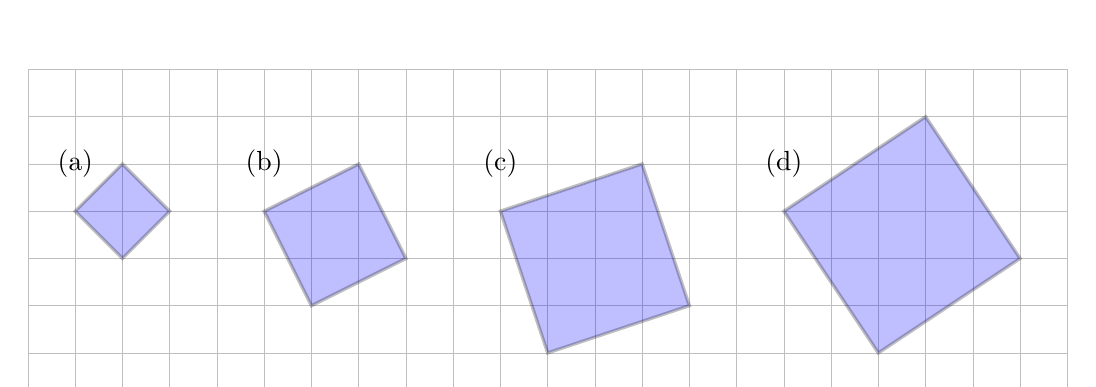
\begin{tikzpicture}[scale=0.6]
	\draw[black!25, very thin] (0,-1) grid (22,6);
	\draw(1,4) node{(a)};
	\draw[very thick, fill=blue, nearly transparent]
		(1,3) -- (2,2) -- (3,3) -- (2,4) -- cycle;
	\draw(5,4) node{(b)};
	\draw[very thick, fill=blue, nearly transparent]
		(5,3) -- (6,1) -- (8,2) -- (7,4) -- cycle;
	\draw(10,4) node{(c)};
	\draw[very thick, fill=blue, nearly transparent]
		(10,3) -- (11,0) -- (14,1) -- (13,4) -- cycle;
	\draw(16,4) node{(d)};
	\draw[very thick, fill=blue, nearly transparent]
		(16,3) -- (18,0) -- (21,2) -- (19,5) -- cycle;
\end{tikzpicture}
\end{center}

What is the area of each square? What is the side length of each square? Can you draw a square with side length $\sqrt{8}$? What about $\sqrt{13}$?

By the way, how do we know that each of these figures is, in fact, a square? (Hint: Think back to the slopes of parallel and perpendicular lines. What argument can we make for why the diagonal segments must be the same length in each figure?)
\end{boxexplore}

As an application of radicals and radical expressions, which are closely connected to the side lengths of squares, it's natural to discuss concepts from geometry. We'll begin with one of the most famous and important statements in mathematics.

\subsection{{P}ythagorean theorem}

It's a good bet that have seen the Pythagorean Theorem before, and that you will see it in every high school mathematics class you take, and many of the mathematics classed you take in college. In fact, the Pythagorean theorem is a foundational piece of an entire branch of mathematics based on the properties of triangles called \textit{trigonometry}.\footnote{Trigonometry begins with the study of triangles. \textit{Trigon} is another way of sayinga \textit{triangle} -- in fact it might be a better way of naming that shape! Most of the other polygons we know (pentagons, hexagons, octagons) have that \textit{-gon} suffix, and the prefix \textit{tri-} means ``three'' (as in tricycle).}

\begin{boxdef}[{P}ythagorean theorem]
The sum of the squares of the lengths of the \glspl{leg} of a right triangle is equal to the square of the length of the \gls{hypotenuse}.

In other words, if $a$ and $b$ represent the lengths of the legs (the perpendicular sides) of a right triangle, and $c$ represents the length of the hypotenuse (the longest side, opposite the right angle), then \[a^2 + b^2 = c^2.\]
\end{boxdef}

The theorem is named after Greek philosopher and mathematician Pythagoras of Samos, who lived around 570--495 BCE.\footnote{\addtodoitem{Need a good Pythagoras footnote.}} However, there is substantial evidence that the theorem was known to many different cultures from many different time periods. There is evidence, for instance, that the ancient Babylonians knew about Pythagorean triples (see the next section) more than 1000 years BCE.

Let's jump in with a famous right triangle: one with legs of length 3 and 4, and with hypotenuse of length 5. If we draw squares on the sides of the triangle, we can see that the sums of the areas of the two smaller squares (9+16) is exactly equal to the area of the largest square (25).
\begin{center}
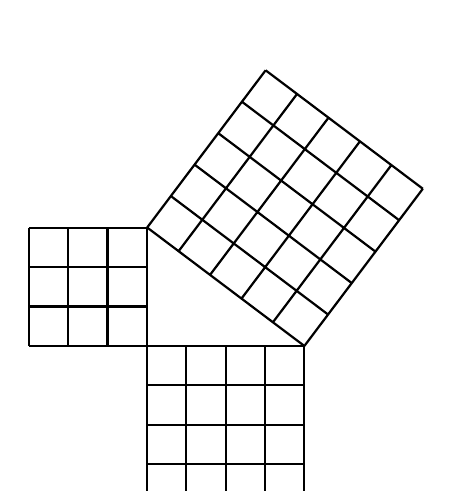
\begin{tikzpicture}[xscale=0.5,yscale=0.5]
	%% grid setup
	%\draw[very thin,color=gray!25] (0,0) grid (12,13);
	\draw[thick] (1,5) grid (4,8);
	\draw[thick] (4,1) grid (8,5);
	\draw[thick,rotate around={53:(8,5)}] (8,5) grid (13,10);
\end{tikzpicture}
\end{center}

This relationship holds true for all right triangles as does its \textit{converse}. The converse of the theorem states that if we have three numbers that satisfy the Pythagorean theorem, then we know that they must form the sides of a right triangle.

You might be asking yourself, ``How do we know that the theorem is true for \textit{every right triangle ever}?'' Those who are curious might enjoy exploring this question at the end of this section.

\subsection{{P}ythagorean triples}

\begin{boxdef}[{P}ythagorean triple]
A \textit{Pythagorean triple} is a set of three positive integers satisfying the Pythagorean theorem.
\end{boxdef}

There are infinitely many Pythagorean triples, and it is quite handy to know a few by heart. (This is because they are used quite a bit in problems, and those delightful standardized tests we all know and love.) Here are a few common Pythagorean triples:
\[
(3, 4, 5) \qquad\qquad
(5, 12, 13) \qquad\qquad
(7, 24, 25) \qquad\qquad
(9, 40, 41) \qquad\qquad
(8, 15, 17)
\]
The benefit of memorizing a few of these is that, if you see that a right triangle that has leg lengths of 7 and 24, you know that the hypotenuse has length 25 without having to do any calculations.

The triples above are called \inlinedef{primitive Pythagorean triples} because the three values are relatively prime. You can generate new Pythagorean triples by scaling up a triple that you know. For example $(6, 8, 10)$ is a triple formed by scaling up the $(3, 4, 5)$ triple by a factor of 2.

\subsubsection{Find-the-missing-side problems}

The classic application of the Pythagorean theorem is to find a missing side length, either a leg or a hypotenuse, and you may have solved problems like this before. Now that we have some algebra skills, however, our answers should be given in simplified radical form! No more decimal approximations (unless the directions state otherwise)!

\begin{boxex}
Find the length of the digaonal of a 4-by-8 rectangle.

\exsoln\ This problem might not, at first, seem to have anything to do with the Pythagorean theorem. The theorem, after all, is about right triangles, and this question is about a rectangle! Drawing a picture helps to reveal the connection:

\begin{center}\begin{tikzpicture}[scale=0.5]
	\draw[dashed] (0,0) -- (8,4);
	\draw (0,0) rectangle (8,4);
	\draw (4,0) node[below]{8};
	\draw (8,2) node[right]{4};
	\draw (4, 2) node[above]{$d$};
\end{tikzpicture}\end{center}

If we let $d$ represent the length of the diagonal, then we can see that it is the hypotenuse of a right triangle with legs of length 4 and 8. So:
\begin{align*}
d^2	&= 4^2 + 8^2
&&\quad\text{Pythagorean theorem}\\
d^2&= 16 + 64\\
d^2&= 80\\
d 	&= \sqrt{80}
&&\quad\text{square root of both sides}\\
d 	&= \sqrt{2 \cdot 2 \cdot 2 \cdot 2 \cdot 5}
&&\quad\text{simplify using the sniper method}\\
d 	&= 2 \cdot 2 \cdot \sqrt{5}\\
d 	&= 4\sqrt{5}
\end{align*}
So, a 4-by-8 rectangle has a diagonal which is $4\sqrt5$ units long.
\end{boxex}

To get a feel for whether this answer is reasonable, we could find a decimal approximation using a calculator (it's about 9 units long, which seems OK), or we could reason as follows. We know that $\sqrt{4} = 2$, and so $\sqrt{5}$ must be a bit more than 2. So, $4\sqrt{5}$ must be a bit more than 8. This seems reasonable.

On the other hand, if we had gotten $4\sqrt{8}$ we might reason that $\sqrt{9} = 3$ and so $4\sqrt{8}$ must be a bit less than $4\sqrt{9} = 4\cdot3 = 12$. This is too long for the diagonal of a 4-by-8 rectangle, since the two sides together are only 12 units long in total!

\subsection{Distance formula}

\begin{boxexplore}[Grid distance]
Find the length of the line segment connecting the points $(1,2)$ and $(6,7)$.
\end{boxexplore}

One important application of the Pythagorean theorem is called the \gls{distance formula}. It is a formula that we can use to calculate the distance between two points on a coordinate grid. In the startup exploration, we have the segment pictured below:

\begin{center}
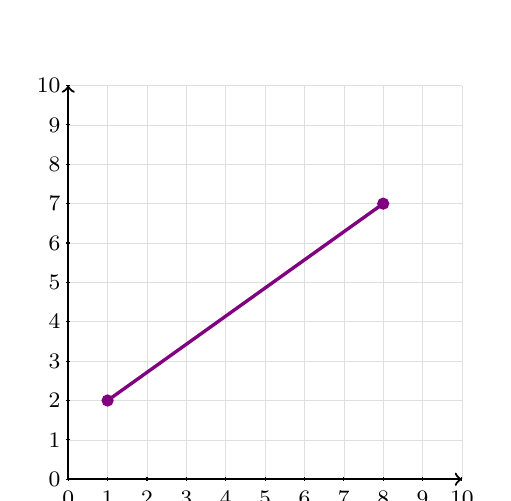
\begin{tikzpicture}[xscale=0.5,yscale=0.5]
	%% grid setup
	\draw[very thin, color=gray!25] (0,0) grid (10,10);
	\draw[->,thick] (0,0) -- (10,0); % node[right] {$x$};
	\draw[->,thick] (0,0) -- (0,10); % node[above] {$y$};
	\foreach \x in {0,...,10} \draw (\x,0.05) -- (\x,-0.05) node[below] {\footnotesize\x};
	\foreach \y in {0,...,10} \draw (-0.05,\y) -- (0.05,\y) node[left] {\footnotesize\y};
	\draw[very thick,violet] (1,2) -- (8,7); % node[right] {$x$};
	\draw[violet] plot[only marks,mark=*,mark size=4] coordinates{(1,2)(8,7)};
\end{tikzpicture}
\end{center}

If we think of the line segment into the hypotenuse of a right triangle, then we can use the Pythagorean theorem! The legs are the vertical and horizontal distances between the points, as in a slope triangle.

Draw the triangle, find the horizontal and vertical distances, then apply the Pythagorean theorem.

\begin{center}
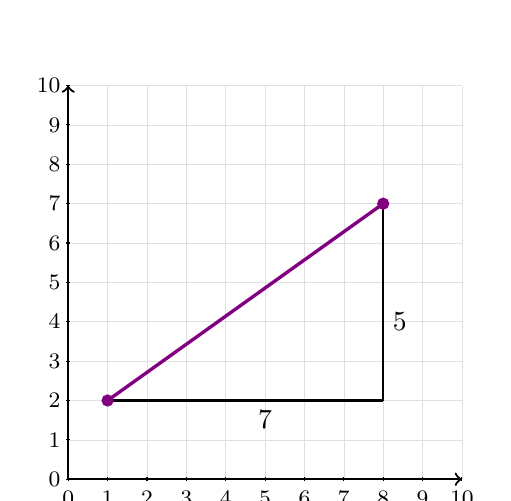
\begin{tikzpicture}[xscale=0.5,yscale=0.5]
	%% grid setup
	\draw[very thin, color=gray!25] (0,0) grid (10,10);
	\draw[->,thick] (0,0) -- (10,0); % node[right] {$x$};
	\draw[->,thick] (0,0) -- (0,10); % node[above] {$y$};
	\foreach \x in {0,...,10} \draw (\x,0.05) -- (\x,-0.05) node[below] {\footnotesize\x};
	\foreach \y in {0,...,10} \draw (-0.05,\y) -- (0.05,\y) node[left] {\footnotesize\y};
	\draw[very thick,violet] (1,2) -- (8,7); % node[right] {$x$};
	\draw[thick] (1,2) -- (8,2);
	\draw (5,2) node[below] {7};
	\draw[thick] (8,2) -- (8,7);
	\draw (8,4) node[right] {5};
	\draw[violet] plot[only marks,mark=*,mark size=4] coordinates{(1,2)(8,7)};
\end{tikzpicture}
\end{center}

The horizontal distance is 7 units, and the vertical distance is 5 units. Those are the legs of the right triangle. Then, we use the theorem to find the length of the hypotenuse: \[\begin{aligned} a^2 + b^2 &= c^2 \\ 5^2 + 7^2 &= c^2 \\ 25 + 49 &= c^2 \\ 74 &= c^2 \\ \sqrt{74} &= c\end{aligned}\]

Since the process is the same every time, we can generalize to find the distance between any two points $(x_1, y_1)$ and $(x_2, y_2)$ in the plane.

\begin{center}
\begin{tikzpicture}[xscale=0.5,yscale=0.5]
	%% grid setup
%	\draw[very thin, color=gray!25] (0,0) grid (10,10);
	\draw[->,thick] (0,0) -- (10,0); % node[right] {$x$};
	\draw[->,thick] (0,0) -- (0,10); % node[above] {$y$};
%	\foreach \x in {0,...,10} \draw (\x,0.05) -- (\x,-0.05) node[below] {\footnotesize\x};
%	\foreach \y in {0,...,10} \draw (-0.05,\y) -- (0.05,\y) node[left] {\footnotesize\y};
	%% line segment
	\draw[very thick,blue] (2,3) -- (8,7); % node[right] {$x$};
	%% horizontal labels
	\draw[dotted] (2,3) -- (2,0);
	\draw (2,0.1) -- (2,-0.1) node[below]{$x_1$};
	\draw[dotted] (8,7) -- (8,0);
	\draw (8,0.1) -- (8,-0.1) node[below]{$x_2$};
	%% vertical labels
	\draw[dotted] (2,3) -- (0,3);
	\draw (0.1,3) -- (-0.1,3) node[left]{$y_1$};
	\draw[dotted] (8,7) -- (0,7);
	\draw (0.1,7) -- (-0.1,7) node[left]{$y_2$};

%	\draw (1,2) node[below]{$(x_1, y_1)$};
%	\draw[thick] (1,2) -- (8,2);
%	\draw (5,2) node[below] {$x_2 - x_1$};
%	\draw[thick] (8,2) -- (8,7);
%	\draw (8,4) node[right] {$y_2 - y_1$};
	\draw[blue] plot[only marks,mark=*,mark size=4] coordinates{(2,3)(8,7)};
\end{tikzpicture}
\end{center}

\begin{boxdef}[Distance formula]
Given two points in the plane $(x_1, y_1)$ and $(x_2, y_2)$, the length $d$ of the line segment connecting the points is given by the formula:
\[d = \sqrt{ (x_2 - x_1)^2 + (y_2 - y_1)^2 }.\]
\end{boxdef}

This might look like a bunch of alphabet soup, much harder to remember than the Pythagorean theorem. But remember: this \textit{is} the Pythagorem theorem! If you forget the formula, don't panic! Just remember that the line segment between the two points is the hypotenuse of a right triangle.

\begin{boxex}
Find the distance between the points $(5, 12)$ and $(-4, -2)$.

\exsoln\ We will use the distance formula, but note that we have both subtraction and negative numbers. Watch those minus signs!
\[\begin{aligned}
d &= \sqrt{ (5 - \umin4)^2 + (12 - \umin2)^2 } \\
&= \sqrt{ 9^2 + 14^2 } \\
&=\sqrt{ 81 + 196 } \\
&=\sqrt{ 277 }
\end{aligned}\]
Since 277 is prime, we know our answer complies with simplified radical form, so we're all done. The distance betnwee the two points is $\sqrt{277}$ units.
\end{boxex}

\subsection{Midpoint formula}

When working with the distance formula, there is a related formula for finding the coordinates of \textit{midpoint} of a given line segment. Suppose we wanted to find the midpoint of the line segment connecting $(2,8)$ and $(8,4)$.
\begin{center}
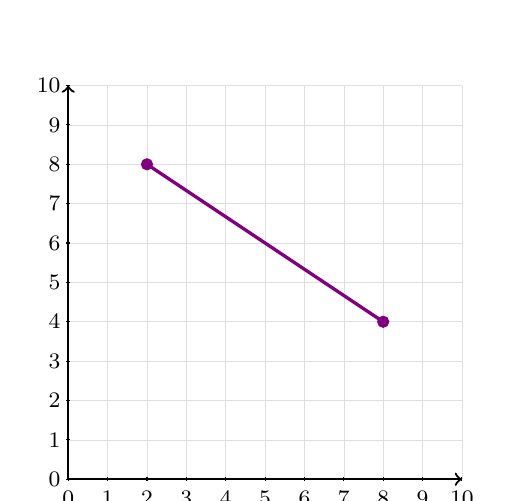
\begin{tikzpicture}[xscale=0.5,yscale=0.5]
	%% grid setup
	\draw[very thin, color=gray!25] (0,0) grid (10,10);
	\draw[->,thick] (0,0) -- (10,0); % node[right] {$x$};
	\draw[->,thick] (0,0) -- (0,10); % node[above] {$y$};
	\foreach \x in {0,...,10} \draw (\x,0.05) -- (\x,-0.05) node[below] {\footnotesize\x};
	\foreach \y in {0,...,10} \draw (-0.05,\y) -- (0.05,\y) node[left] {\footnotesize\y};
	\draw[very thick,violet] (2,8) -- (8,4); % node[right] {$x$};
	\draw[violet] plot[only marks,mark=*,mark size=4] coordinates{(2,8)(8,4)};
\end{tikzpicture}
\end{center}
Well, it sure looks like the midpoint of this segment is the point $(5,6)$\ldots\ but can we be sure?

One way to explain this is by drawing in the right triangle, and then chopping that triangle into four congruent sub-triangles. (Remember our work with the Sierpi\'{n}ski triangle ages ago?)
\begin{center}
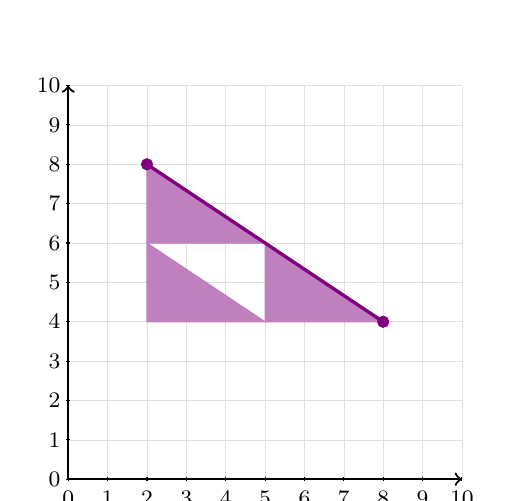
\begin{tikzpicture}[xscale=0.5,yscale=0.5]
	%% grid setup
	\draw[very thin, color=gray!25] (0,0) grid (10,10);
	\draw[->,thick] (0,0) -- (10,0); % node[right] {$x$};
	\draw[->,thick] (0,0) -- (0,10); % node[above] {$y$};
	\foreach \x in {0,...,10} \draw (\x,0.05) -- (\x,-0.05) node[below] {\footnotesize\x};
	\foreach \y in {0,...,10} \draw (-0.05,\y) -- (0.05,\y) node[left] {\footnotesize\y};
	\draw[violet!50, fill=violet!50] (2,8)--(2,6)--(5,6)--cycle;
	\draw[violet!50, fill=violet!50] (2,6)--(2,4)--(5,4)--cycle;
	\draw[violet!50, fill=violet!50] (5,6)--(5,4)--(8,4)--cycle;
	\draw[very thick,violet] (2,8) -- (8,4); % node[right] {$x$};
	\draw[violet] plot[only marks,mark=*,mark size=4] coordinates{(2,8)(8,4)};
\end{tikzpicture}
\end{center}
This diagram suggests that the $x$-coordinate of the midpoint of the hypotenuse is exactly halfway between the $x$-coordinates of the legs. The same goes for the $y$-coordinate. So, to find the coordinates of the midpoint, all we have to do is average the coordinates of the endpoints! Once again, you don't have to memorize this formula if you remember where it comes from!


\begin{boxdef}[Midpoint formula]
Given a line segment with endpoints $(x_1, y_1)$ and $(x_2, y_2)$, the coordinates of the midpoint of the segment are \[\left( \frac{x_1+x_2}{2} ~,~ \frac{y_1+y_2}{2} \right)\]
\end{boxdef}

\begin{boxex}
Find the midpoint of the segment connecting the points $(-13,8)$ and $(6, -2)$.

\inlineex{Solution:} Let's calculate the midpont first, and then check our answer by drawing a picture. The formula is pretty straightforward. The midpoint should be located at: \[\left( \frac{-13+6}{2} ~,~ \frac{8+\umin2}{2} \right) = \left( \frac{-7}{2} ~,~ \frac{6}{2} \right) = (-3.5, 3) \]
Here's a graph to check that our answer is reasonable:
\begin{center}
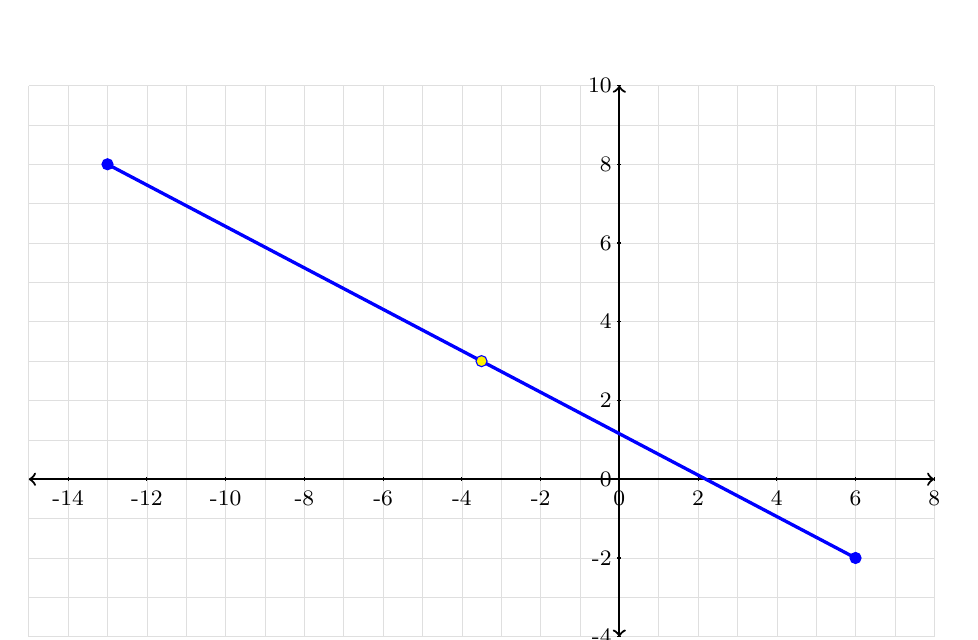
\begin{tikzpicture}[scale=0.5]
	%% grid setup
	\draw[very thin, color=gray!25] (-15,-4) grid (8, 10);
	\draw[<->,thick] (-15,0) -- (8,0);
	\draw[<->,thick] (0,-4) -- (0,10);
	\foreach \x in {-14,-12,...,8} \draw (\x,0.05) -- (\x,-0.05) node[below] {\footnotesize\x};
	\foreach \y in {-4,-2,...,10} \draw (-0.05,\y) -- (0.05,\y) node[left] {\footnotesize\y};
	%% line segment
	\draw[very thick,blue] (-13,8)--(6,-2);
	\draw[blue] plot[only marks,mark=*,mark size=4] coordinates{(-13,8)(6,-2)};
	\draw[blue, fill=yellow] plot[only marks,mark=*,mark size=4] coordinates{(-3.5,3)};
\end{tikzpicture}
\end{center}
\end{boxex}

\subsection{(;,;) Proof of the {P}ythagorean theorem}
\label{sec:pythagproof}

Imagine a pizza box and four identical slices of pizza\ldots\ where the pizza slices are right triangles. (Not typical for pizza slices, we know, but go with it.)

\begin{center}
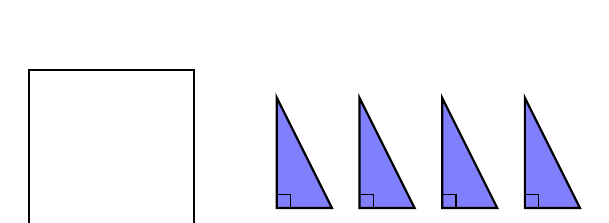
\begin{tikzpicture}[scale=0.35]
	\draw[thick] (0,0) rectangle (6,6);
	\foreach \x in {9,12,15,18} {
		\draw[thick, fill=blue!50] (\x,1) -- (\x+2,1) -- (\x,5) -- cycle;
		\draw (\x,1) rectangle (\x+0.5, 1.5);
	}
\end{tikzpicture}
\end{center}

Consider two different arrangements of the same four pizza slices inside the same pizza box. The slices are arranged to that they fit inside without overlapping, and they lay flat on the bottom of the box.

\begin{center}
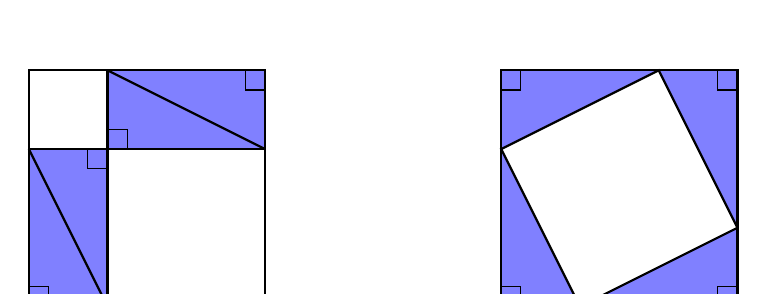
\begin{tikzpicture}[scale=0.5]
	%% Box 1
	\draw[thick] (0,0) rectangle (6,6);
	\draw[thick,fill=blue!50] (0,0) rectangle (2,4);
	\draw[thick,fill=blue!50] (2,4) rectangle (6,6);
	\draw (0,0) rectangle (0.5, 0.5);
	\draw (2,4) rectangle (1.5, 3.5);
	\draw (2,4) rectangle (2.5, 4.5);
	\draw (6,6) rectangle (5.5, 5.5);
	\draw[thick] (0,4) -- (2,0);
	\draw[thick] (2,6) -- (6,4);
	%% Box 2
	\begin{scope}[xshift=12cm]
	\draw[thick,fill=blue!50] (0,0) rectangle (6,6);
	\draw (0,0) rectangle (0.5, 0.5);
	\draw (0,6) rectangle (0.5, 5.5);
	\draw (6,0) rectangle (5.5, 0.5);
	\draw (6,6) rectangle (5.5, 5.5);
	\draw[thick,fill=white] (0,4) -- (2,0) -- (6,2) -- (4,6) -- cycle;
	\end{scope}
\end{tikzpicture}
\end{center}

\textit{Step 1:~} Consider the image on the left: Write an expression for the area of the box that is left \textit{uncovered}. You may find it helpful to label the sides of the triangles, or the sides of the box (or both).

You may be tempted to say that the uncovered regions are squares. How do we know -- for sure -- that these two regions are actually \textit{squares}, as opposed to some other quadrilateral?

\textit{Step 2:~} Consider the image on the right: Write an expression for the area of the box that is left \textit{uncovered}. Use the same labels you assigned when studying the other picture.

Again, you may be tempted to say that the uncovered region is a square. How do we know that it is a square (and not, say, a rhombus)?

\textit{Step 3:~} The area that is uncovered by the pizza slices is the same. (How do we know this?) What does this tell us about the two expressions for the uncovered area?

\subsubsection{Alternative approach}

In fact, we can explain the theorem using only the right-hand diagram. Let $a$ and $b$ be the lengths of the legs of one of the triangles, and let $c$ be the length of the hypotenuse.

\begin{center}
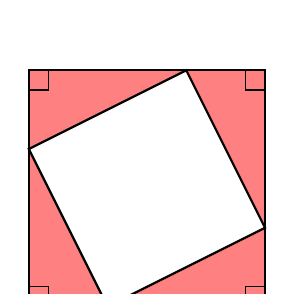
\begin{tikzpicture}[scale=0.5]
	%% Box 2
	\draw[thick,fill=red!50] (0,0) rectangle (6,6);
	\draw (0,0) rectangle (0.5, 0.5);
	\draw (0,6) rectangle (0.5, 5.5);
	\draw (6,0) rectangle (5.5, 0.5);
	\draw (6,6) rectangle (5.5, 5.5);
	\draw[thick,fill=white] (0,4) -- (2,0) -- (6,2) -- (4,6) -- cycle;
\end{tikzpicture}
\end{center}

\textit{Step 1:~} Express the sides of the largest square (the pizza box itself) in terms of $a$ and $b$.

\textit{Step 2:~} Express the area of the largest square in terms of $a$ and $b$. (Hint: You'll need the sum to a power rule.)

\textit{Step 3:~} The area of the largest square can also be expressed at the sum of the areas of the four triangles plus the area of the tiled square. Express the area of the largest square in this way (in terms of $a$, $b$, and $c$).

\textit{Step 4:~} We now have two ways of expressing the area of the largest square. What happens when set them equal to each other?

\subsubsection{Generalizing}

All the figures in this discussion have been drawn using a particular square and a particular triangle. Explain why these arguments are proof that the Pythagorean theorem is true for any right triangle, not just the specific triangle that is pictured in these diagrams.


% % % % % % % % % % % % % % % % % % % % % % % % % % % % % % % % % % % % % % % % 
\chaptersummary

Our algebra toolbox grows ever larger! We can now handle the simplification of numerical expressions that include square roots. This, combined with our work from the previous chapter, means that we can handle even the most ``impolite'' of quadratic equations. Plus, along the way we have discovered some fundamental results from geometry.

These skills are valuable, without a doubt, but we haven't looked closely at quadratic functions in detail. These are the focus of the next chapter. Onward!

\chaptercopyright

\include{ch14_quadfunc}
\include{ch15_polynomials}
\include{ch16_factoring}

% Appendices
\appendix
\newcounter{primeHctr}
\include{appA_primes}

% % % % % % % % % % % % % % % % % % % % % % % % % % % % % % % % % % % % % % % % 
% 
% BACK MATTER
%
\backmatter
\pagestyle{plain}

\include{ab_backmatter}

\clearpage

% Close output stream for to-do list
\immediate\closeout\outputstream

\end{document}
